\documentclass[11pt,twoside,a4paper]{book}
%
% Unitex/GramLab manual
%
\usepackage[utf8]{inputenc}
\usepackage[T1]{fontenc}
\usepackage[frenchb]{babel}
\selectlanguage{french}
\usepackage{hyphenat}
\frenchbsetup{StandardLists=true}
\usepackage{palatino}
\usepackage{epsfig}
%The following line translates the \see macro of makeidx into French. Not sure it should be here
\newcommand{\voir}[2]{\emph{voir} #1}
\usepackage{graphicx}
\usepackage{float}
\usepackage{longtable}
\usepackage{fancyvrb}
\usepackage[nodayofweek]{datetime}
\newdateformat{mydate}{\twodigit{\THEDAY}{ }\monthname[\THEMONTH] \THEYEAR}
%----------------------------------------------------------------------------- %
% THIS FILE MAY BE OVERWRITTEN BY THE BUILDING SERVICE USING VERSION.TEX.IN
%----------------------------------------------------------------------------- %
% Release information
% e.g. Unitex/GramLab
\newcommand{\UnitexAppName}{\verbl{Unitex/GramLab}}
% e.g. Unitex/GramLab 3.3rc
\newcommand{\UnitexRelease}{\verbl{Unitex/GramLab 3.3rc}}
% e.g. Unitex/Gramlab 3.3rc Rev. 3816
\newcommand{\UnitexFullRelease}{\verbl{Unitex/GramLab 3.3rc}}
%----------------------------------------------------------------------------- %
% Version information
% e.g. 3.3rc
\newcommand{\UnitexVersion}{\verbl{3.3rc}}
% e.g. 3
\newcommand{\UnitexVersionMajor}{\verbl{3}}
% e.g. 1
\newcommand{\UnitexVersionMinor}{\verbl{3}}
% e.g. 3816
\newcommand{\UnitexVersionRevision}{\verbl{0}}
% e.g. rc
\newcommand{\UnitexVersionSuffix}{\verbl{rc}}
% e.g. 3.3rc Rev. 3816
\newcommand{\UnitexVersionString}{\verbl{3.3rc}}
% e.g. 3.3.3816-rc
\newcommand{\UnitexSemVer}{\verbl{3.3.0-rc}}
%----------------------------------------------------------------------------- %
% Package names
% e.g. Unitex-GramLab
\newcommand{\UnitexPackageName}{\verbl{Unitex-GramLab}}
% e.g. Unitex-GramLab-3.3rc_win32-setup.exe
\newcommand{\UnitexPackageWin}{\verbl{Unitex-GramLab-3.3rc_win32-setup.exe}}
% e.g. Unitex-GramLab-3.3rc_win64-setup.exe
\newcommand{\UnitexPackageWinSF}{\verbl{Unitex-GramLab-3.3rc_win64-setup.exe}}
% e.g. Unitex-GramLab-3.3rc-linux-i686.run
\newcommand{\UnitexPackageLinux}{\verbl{Unitex-GramLab-3.3rc-linux-i686.run}}
% e.g. Unitex-GramLab-3.3rc-linux-x86_64.run
\newcommand{\UnitexPackageLinuxSF}{\verbl{Unitex-GramLab-3.3rc-linux-x86_64.run}}
% e.g. Unitex-GramLab-3.3rc-osx.run
\newcommand{\UnitexPackageOSX}{\verbl{Unitex-GramLab-3.3rc-osx.run}}
% e.g. Unitex-GramLab-3.3rc-source-distribution.zip
\newcommand{\UnitexPackageSource}{\verbl{Unitex-GramLab-3.3rc-source-distribution.zip}}
%----------------------------------------------------------------------------- %
% URLs
% e.g. https://unitexgramlab.org
\newcommand{\UnitexURLWebsite}{https://unitexgramlab.org}
% e.g. http://releases.unitexgramlab.org
\newcommand{\UnitexURLReleases}{http://releases.unitexgramlab.org}
% e.g. http://releases.unitexgramlab.org/latest-rc
\newcommand{\UnitexURLLatestReleases}{http://releases.unitexgramlab.org/latest-rc}
% e.g. http://code.unitexgramlab.org
\newcommand{\UnitexURLSources}{http://code.unitexgramlab.org}
% e.g. http://forum.unitexgramlab.org
\newcommand{\UnitexURLForum}{http://forum.unitexgramlab.org}
% e.g. http://governance.unitexgramlab.org
\newcommand{\UnitexURLGovernance}{http://governance.unitexgramlab.org}
%----------------------------------------------------------------------------- %


\usepackage{comment}
\title{Unitex \UnitexVersion{} User Manual}
\author{Sébastien Paumier - Université Paris-Est Marne-la-Vallée}
\date{2015}


\usepackage[%
%%              ps2pdf,
%%              dvips,
             pdfauthor={Sébastien Paumier},
             pdftitle={Manuel d'utilisation d'Unitex},
             pdfcreator={LaTeX, hyperref},
             pdfkeywords={corpus linguistics, computational linguistics,
             finite state automata / transducer, local grammar, lexicon grammar}, pdfsubject={Manual of Unitex, a corpus processing system, based on automata-oriented technology},
             %final, % use hyperlinks ever
             bookmarks,
             backref,
%%              breaklinks=true,
             colorlinks=true,
             urlcolor=blue,
%%              linkcolor=black,
%%              citecolor=black,
%%              anchorcolor=black,
             pdfpagemode=None,
           % pdfpagemode=FullScreen,
             pdfstartview=FitBH,
             unicode,
             hyperindex=false
             ]{hyperref}

% put always after hyperref
\usepackage[xindy]{imakeidx}

%
% définitions de commandes
%
%\newcommand{\httplink}[1]{\textcolor{blue}{\underline{\texttt{http://#1}}}}
\newcommand{\E}{$\varepsilon$}
\newcommand{\exemplemauvais}[1]{\textit{* #1}}
\newcommand{\exemplebon}[1]{\textit{#1}}
\newcommand{\exemplebizarre}[1]{\textit{? #1}}
\newcommand{\exempletresbizarre}[1]{\textit{*? #1}}
\newcommand{\targetindexentry}[1]{\hypertarget{index:#1}{#1}}
\newcommand{\seelink}[1]{\hyperlink{index:#1}{\see{#1}}}
% use without escaping special chars
\newcommand{\verbc}[1]{\texttt{\detokenize{#1}}}
% use escaping special chars
\newcommand{\verbt}[1]{\texttt{#1}}
% light verb without monospace font
\newcommand{\verbl}[1]{\detokenize\expandafter{#1}}
\pagenumbering{arabic}
\global\setlength{\topmargin}{-1.5cm}
\global\setlength{\footskip}{2cm}
\global\setlength{\headheight}{1.5cm}
\global\setlength{\headsep}{0.3cm}
\global\setlength{\textheight}{21.5cm}
\global\setlength{\oddsidemargin}{0.5cm}
\global\setlength{\evensidemargin}{0.5cm}
\global\setlength{\marginparwidth}{1.5cm}
\global\setlength{\textwidth}{15.5cm}

\def\xindyopts{-L french}
\makeindex[options=\xindyopts]

%\frenchbsetup{ReduceListSpacing=false}
%\global\setlength{\itemsep}{20pt}

% Hyphenation rules
% Use \showhyphens{développement} to show default hyphens
%--------------------------------------
%\hyphenation{ma-ni-pu-lées nor-ma-li-sa-tion}
%--------------------------------------

\begin{document}


\begin{titlepage}
\begin{center}

~

\vspace{3cm}
\Huge
\textsc{\textbf{Unitex \UnitexVersion{}}}

\vspace{1cm}

\huge
\textsc{\textbf{Manuel d'utilisation}}

\vspace{2cm}

  \begin{center}
    \includegraphics[width=4cm]{resources/img/logo-Unitex.png}
  \end{center}
\normalsize

\vspace{2cm}

\LARGE

Université Paris-Est Marne-la-Vallée
\bigskip
\normalsize

\url{http://unitexgramlab.org}

\verb$unitex-devel@univ-mlv.fr$

\vspace{1cm}

Sébastien Paumier
\bigskip

avec la participation de Wolfgang Flury, Franz Guenthner, Eric Laporte,\\
Friederike Malchok, Clemens Marschner, Claude Martineau, Denis Maurel,\\
Sebastian Nagel, Alexis Neme, Maxime Petit, Johannes Stiehler, Gilles Vollant\\
\bigskip

% Mise à jour automatique de la date
\mydate
Date de cette version~: \today
\end{center}

\end{titlepage}


\tableofcontents

\chapter*{Introduction}
\addcontentsline{toc}{chapter}{Introduction}

Unitex est un ensemble de logiciels permettant de traiter des textes en langues naturelles en
utilisant des ressources linguistiques. Ces ressources se présentent sous la forme de dictionnaires
électroniques, de grammaires et de tables de lexique-grammaire. Elles sont issues de travaux initiés
sur le français par Maurice Gross au Laboratoire d’Automatique Documentaire et Linguistique (LADL)
. \index{LADL} Ces travaux ont été étendus à d’autres langues au travers du réseau de laboratoires
RELEX.

\bigskip
\noindent Les dictionnaires électroniques décrivent les mots simples et composés d’une langue en
leur associant un lemme ainsi qu’une série de codes grammaticaux, sémantiques et flexionnels. La présence de ces dictionnaires constitue une différence majeure par rapport aux outils
usuels de recherche de motifs, car on peut faire référence aux informations qu’ils contiennent
et ainsi décrire de larges classes de mots avec des motifs très simples. Ces dictionnaires sont
représentés selon le formalisme DELA et ont été élaborés par des équipes de linguistes pour
plusieurs langues (français, anglais, grec, italien, espagnol, allemand, thaï, coréen, polonais,
norvégien, portugais, etc...).


\bigskip
\noindent Les grammaires sont des représentations de phénomènes linguistiques par réseaux de
transitions récursifs (RTN), un formalisme proche de celui des automates à états finis. De
nombreuses études ont mis en évidence l’adéquation des automates aux problèmes linguistiques et ce,
aussi bien en morphologie qu’en syntaxe ou en phonétique. Les grammaires manipulées par Unitex
reprennent ce principe, tout en reposant sur un formalisme encore plus puissant que les automates.
Ces grammaires sont représentées au moyen de graphes que l’utilisateur peut aisément créer et
mettre à jour.

\bigskip
\noindent Les tables de lexique-grammaire sont des matrices décrivant les propriétés de certains
mots. De telles tables ont été élaborées pour tous les verbes simples du français dont elles
décrivent les propriétés syntaxiques. L’expérience ayant montré que chaque mot a un comportement
quasi unique, ces tables permettent de donner la grammaire de chaque élément de lexique, d’où le nom
de lexique-grammaire. Unitex permet de construire des grammaires à partir de telles tables.

\bigskip
\noindent Unitex est un moteur permettant d’exploiter ces ressources linguistiques. Ses
caractéristiques techniques sont la portabilité, la modularité, la possibilité de gérer des langues
possédant des systèmes d’écritures particuliers comme certaines langues asiatiques et l’ouverture,
grâce à une distribution en logiciel libre. Ses caractéristiques linguistiques sont celles
qui ont motivé l’élaboration des ressources : la précision, l’exhaustivité et la prise en compte
des phénomènes de figement, notamment en ce qui concerne le recensement des mots com-
posés.




\section*{Quoi de neuf depuis la version 3.2~?}
\addcontentsline{toc}{section}{Quoi de neuf depuis la version 3.2~?}
Voici les principales nouvelles fonctionnalités:
\begin{itemize}
  \item Le module Unxmlize (section~\ref{section-Unxmlize}) a de
  nouvelles fonctionnalités.
  \item L'exploration des chemins des grammaires (section~\ref{explore-paths}) a de nouvelles fonctionnalités.
  \item Quelques anomalies ont été corrigées et la qualité du code
  en certains points a été améliorée. 
\end{itemize}

\noindent Merci à Cristian Martínez, Gilles Vollant, Denis Biguenet, Jean-Manuel Erialc et Fabien Lambert-Delavaquerie pour leur contribution.

%\clearpage

\section*{Contenu}
\addcontentsline{toc}{section}{Contenu}
\noindent Le chapitre \ref{chap-install} décrit comment installer et lancer Unitex.

\bigskip \noindent Le chapitre \ref{chap-text} présente les différentes étapes de l'analyse d'un
texte.

\bigskip \noindent Le chapitre \ref{chap-dictionaries} décrit le formalisme 
des dictionnaires électroniques DELA et les différentes opérations qui peuvent leur être appliqués.

\bigskip \noindent Les chapitres \ref{chap-regexp} et \ref{chap-grammars}
présentent les différents moyens d’effectuer des recherches de motifs dans des textes.
Le chapitre \ref{chap-grammars} décrit en détail l'utilisation de l'éditeur de graphe.

\bigskip \noindent Le chapitre \ref{chap-advanced-grammars} est consacré aux différentes
utilisations possibles des grammaires. Les particularités de chaque type de grammaires y sont
présentées.

\bigskip \noindent Le chapitre \ref{chap-text-automaton} présente le concept d'automate du texte 
et décrit les propriétés de cette notion. Ce chapitre  décrit également les opérations sur cet
objet, en particulier, comment désambiguiser les items lexicaux avec le programme ELAG.

\bigskip \noindent Le chapitre \ref{chap-lexicon-grammar} contient une présentation des tables du
lexique-grammaire, et la description d'une méthode de construction de  grammaires fondées sur ces
tables.

\bigskip \noindent Le chapitre \ref{chap-alignment} décrit le module d'alignement de texte basé sur
l'outil XAlign.

\bigskip \noindent Le chapitre \ref{chap-multiflex} décrit le module de flexion des mots composés,
en tant que complément du système de flexion des mots simples, présenté au chapitre
\ref{chap-dictionaries}.

\bigskip \noindent Le chapitre \ref{chap-cassys} décrit le système de cascades de transducteurs
CasSys.

\bigskip \noindent Le chapitre \ref{chap-scripts} explique comment utiliser Unitex/GramLab
par l'intermédiaire de scripts qui lancent des programmes.

\bigskip \noindent Le chapitre \ref{chap-external-programs} contient une description détaillée des
programmes externes qui composent le système Unitex.

\bigskip \noindent Le chapitre \ref{chap-file-formats} contient une description de tous les formats
de fichiers utilisés par Unitex.


\bigskip \noindent Le lecteur trouvera en annexe la licence LGPL sous  laquelle le code source
Unitex est diffusé, ainsi que la licence LGPLLR qui s'applique pour les données linguistiques
distribuées avec Unitex. Il y trouvera aussi la licence 2-clause BSD qui s'applique à la
bibliothèque TRE, utilisée par Unitex pour les filtres morphologiques.

%\clearpage

\section*{Contributions à Unitex}
\addcontentsline{toc}{section}{Contributions à Unitex}
Unitex est né comme un pari sur la puissance de la philosophie Open Source dans le monde
universitaire (voir \url{http://unitexgramlab.org/why-unitex}), en s'appuyant sur l'hypothèse que les gens seraient intéressés à partager leurs connaissances et leurs compétences dans un tel projet ouvert.
La liste ci-dessous laisse penser que l'open source fait avancer les sciences:
%The following list sounds like Open Source is good for science:

\begin{itemize}                   
    \item Olivier Blanc: a intégré le système ELAG à Unitex, originellement conçu par Eric Laporte,
    Anne Monceaux et certains de leurs étudiants, a également écrit \verb+RebuildTfst+ (anciennement
     appelé \verb+MergeTextAutomaton+)
    \item Matthieu Constant: auteur de \verb+Grf2Fst2+
    \item Julien Decreton: auteur de l'éditeur de texte intégré à Unitex,
    	    a aussi réalisé la fonctionnalité \verb+undo+ de l'éditeur de graphe
    \item Marwin Damis: amélioration de l'interface de l'automate du texte
    \item Claude Devis: ajout des filtres morphologiques, fondé sur la bibliothèque TRE
    \item Nathalie Friburger: auteure de \verb+CasSys+
    \item Anubhav Gupta: a perfectionné \verb+CasSys+
    \item Hyun-Gue Huh: auteur de l'outil de génération de dictionnaires coréens
    \item Claude Martineau: a travaillé sur la flexion des mots simples dans \verb+MultiFlex+
    \item Cristian Martínez: a mis en place la chaine d'intégration continue et corrigé des anomalies
    importantes
    \item  Renaud Mouronval: a amélioré l'exploration des chemins des grammaires
    \item Sebastian Nagel: a optimisé de nombreuses parties du code, il a également adapté
    	    \verb+PolyLex+ pour l'allemand et le russe
    \item Alexis Neme: a optimisé \verb+Dico+ et \verb+Tokenize+, a aussi intégré \verb+Locate+
    dans \verb+Dico+ pour accepter des graphes dictionnaires
     \item Aljosa Obuljen: auteur de \verb+Stats+
     \item Sébastien Paumier: développeur principal
    \item Maxime Petit: a amélioré la fonctionnalité "rechercher et remplacer" pour les graphes
     \item Agata Savary: auteure de \verb+MultiFlex+
    \item Anthony Sigogne: auteur de \verb+Tagger+ et de \verb+TrainingTagger+
    \item Gilles Vollant: auteur de \verb+UnitexTool+, a optimisé beaucoup
    	    d'aspects du code d'Unitex (mémoire, vitesse, compatibilité multi-compilateur, etc.) et corrigé
    	    d'innombrables anomalies
    \item Patrick Watrin: auteur de \verb+XMLizer+, a travaillé sur l'intégration de \verb+XAlign+ à Unitex
    \item Anthony Sigogne: auteur de \verb+Tagger+ et de \verb+TrainingTagger+
\end{itemize}

\bigskip
\noindent Il faut ajouter que Unitex serait inutile sans les précieuses ressources linguistiques
qu'il renferme. Toutes ces ressources sont le fruit d'un énorme et difficile travail effectué par
des personnes qui ne doivent pas être oubliées. Certaines sont citées dans les avertissements qui
sont fournis avec les dictionnaires, une information complète est disponible sur:

\bigskip
\noindent \url{http://unitexgramlab.org/language-resources}


\section*{Si vous utilisez Unitex dans des projets de recherche...}
\addcontentsline{toc}{section}{Si vous utilisez Unitex dans des projets de recherche...}
Unitex a été utlisé dans plusieurs projets de recherche. Certains sont listés dans la section 
``Related works'' de la page d'accueil d'Unitex. Si vous avez effectuer des travaux de recherche
avec Unitex (ressources, projet, article, thèse, ...) et si vous désirez qu'ils soient référencés
sur le site envoyez un mail à \url{unitex-devel@univ-mlv.fr}.


\chapter{Installation d'Unitex}
\label{chap-install}

Unitex est un système multi-plateformes capable de fonctionner aussi bien sous
Windows que sous Linux ou OS~X. Ce chapitre décrit l’installation et le lancement d’Unitex
pour chacun de ces systèmes. Il présente également les procédures d’ajout de nouvelles
langues et de désinstallation.

\section{Licences}
\label{section-licences}
\index{Licence!LGPL}\index{Licence!LGPL}
Unitex est un logiciel libre. Cela signifie que le code source des programmes est distribué avec le
logiciel, et que chacun peut le modifier et le redistribuer. Le code des programmes d’Unitex est
sous licence LGPL (\cite{LGPL}), à l’exception de~:

\begin{enumerate}
\item la bibliothèque de manipulation d’expressions régulières TRE de Ville Laurikari (\cite{TRE}),
qui est sous une licence du genre des licences BSD à 2 clauses~;

\item la bibliothèque \verb+wingetopt+ de Todd Miller et de la Fondation NetBSD, également sous une licence
 du genre des licences BSD à 2 clauses, plus permissive que la licence LPGL~;

\item l'analyseur syntaxique Xerces2 Java Parser, de l'Apache Software Foundation, sous licence Apache~;

\item  la bibliothèque LibYAML de Kirill Simonov, qui est sous licence MIT, également plus permissive que la licence LGPL~;

\item la bibliothèque SVNKit de TMate Software, sous licence TMate.
\end{enumerate}

\noindent La licence LGPL est plus permissive que la licence GPL, car elle permet d’utiliser du code LGPL dans
des logiciels non libres. Dans les deux cas, le logiciel peut librement être utilisé et distribué.


\bigskip
\noindent Toutes les ressources linguistiques distribuées avec Unitex sont soumises à la licence LGPLLR
\index{Licence!LGPLLR} (\cite{LGPLLR}).

\bigskip
\noindent Le texte complet des licences LGPL, BSD à 2 clauses, Apache, MIT, TMate et LGPLLR
se trouve dans les annexes à la fin de ce manuel.

\section{Environnement d’exécution Java}
Unitex est composé d’une interface graphique écrite en Java et de programmes externes
écrits en \textit{C/C\kern-.05em\raisebox{.5ex}{++}\kern-.1em}. Ce mélange de langages de 
programmation permet d’avoir une application rapide et portable sous différents systèmes d’exploitation.


\bigskip
\noindent Afin de pouvoir utiliser l’interface graphique, il faut préalablement installer
un environnement d’exécution, communément appelé machine virtuelle \index{Java!machine virtuelle} ou
JRE\index{JRE} (Java Runtime Environment\index{Java!Runtime Environment}\index{Java!JRE}).

\bigskip
\noindent Pour fonctionner en mode graphique, Unitex nécessite une version 1.7 (ou plus récente)
de Java. Si vous avez une version trop ancienne de Java, Unitex se bloquera après que vous
ayez choisi votre langue de travail.


\bigskip
\noindent Vous pouvez télécharger librement la machine virtuelle correspondant à votre 
système d’exploitation sur le site de Sun Microsystems (\cite{site-java}) à l’adresse suivante : 
\url{http://java.sun.com}.

\bigskip
\noindent Si vous travaillez sous Linux ou OS X, ou si vous
utilisez une version de Windows gérant des comptes personnels pour les utilisateurs, il vous
faudra demander à votre administrateur système d’installer Java.


\section{Programme d'installation}
\begin{samepage}
\index{Fichier!d'installation}
Le programme d'installation d'Unitex/GramLab peut être téléchargé depuis cette page~:

\begin{center}
{\tt\url{\UnitexURLLatestReleases}}
\end{center}
\end{samepage}

\subsection{Sous Windows}
\index{Installation!sous Windows}
Le nom du fichier téléchargé sera par exemple~:

\begin{flushleft}
{\tt \UnitexPackageWin{}}
{\tt \UnitexPackageWinSF{}}
\end{flushleft}

\noindent Ensuite, double-cliquez sur ce fichier et suivez les instructions (fig.~\ref{fig-installer}).
Il est recommandé de désinstaller
toute version existante avant d'en installer une nouvelle. Unitex/GramLab sera installé
dans un répertoire (dossier)\index{Dossier|see{Répertoire}} situé
de préférence dans le répertoire  \verb+Program Files+, et qui sera appelé dans ce manuel
le répertoire système Unitex.\index{Répertoire!système Unitex}

\begin{figure}[!ht]
\begin{center}
\includegraphics[width=13cm]{resources/img/installer.png}
\caption{Programme d'installation sous Windows\label{fig-installer}}
\end{center}
\end{figure}


\bigskip
\noindent Une fois l'installation terminée, une icône Unitex et une icône GramLab apparaissent
sur le bureau~: double-cliquez dessus pour lancer Unitex ou GramLab (voir~\ref{section-first-use}).
(Si le programme d'installation n'a pas créé ces icônes, ouvrez le répertoire Unitex système~: il contient
plusieurs sous-répertoires, dont un est \verb+App+.  Ce dernier répertoire contient deux fichiers
\verb+Unitex.jar+\index{Fichier!\verbc{Unitex.jar}} et \verb+GramLab.jar+.
 Ce sont les fichiers Java qui lancent les interfaces graphiques. Double-cliquez sur l'un d'entre eux
pour lancer Unitex ou GramLab (voir~\ref{section-first-use}).
Pour faciliter le lancement du programme, il est conseillé de créer des raccourcis vers ces fichiers sur le bureau.)

\bigskip
\noindent Si vous désirez installer Unitex sur une machine Windows multi-utilisateurs, il est
préférable de demander à votre administrateur de le faire. Si vous êtes le seul utilisateur de
votre machine, vous pouvez effectuer l’installation vous-même.

\bigskip
\begin{samepage}
\noindent Le programme d'installation sous Windows peut aussi être lancé en ligne de commande et dans ce cas
il accepte plusieurs paramètres optionnels. En voici quelques-uns~:

\begin{itemize}
\itemsep1pt\parskip0pt\parsep0pt
\item
  \texttt{/AllUsers} \hspace{.15in} Par défaut i'installation vaudra pour tous les utilisateurs\\
\item
  \texttt{/CurrentUser} \hspace{.15in} Par défaut i'installation vaudra pour l'utilisateur seulement\\
\item
  \texttt{/D C:\textbackslash{}path\textbackslash{}without quotes\textbackslash{}} \hspace{.15in}
  Spécifie le répertoire d'installation par défaut\\
\item
  \texttt{/NCRC} \hspace{.15in} Saute le contrôle de redondance cyclique\\
\item
  \texttt{/S} \hspace{.15in} Supprime toutes les questions
\end{itemize}
\end{samepage}

\noindent Sous Windows~7, on peut avoir des problèmes avec le fichier de configuration d'Unitex, car Unitex
essaie de le créer dans le sous-répertoire Unitex et Windows~7 le lui interdit.

\subsection{Sous GNU/Linux et OS~X}
\index{Installation!sous Linux}\index{Installation!sous OS X}
Le nom du fichier téléchargé sera par exemple~:

\begin{flushleft}
{\tt \UnitexPackageLinux{}}
{\tt \UnitexPackageLinuxSF{}}
\end{flushleft}

\noindent Donnez-lui les droits d'exécution, par exemple par~:

\begin{flushleft}
{\tt chmod a+x \UnitexPackageLinux{}}
\end{flushleft}

\noindent Le fichier \verb+.run+ est une archive qu'on décompresse en l'exécutant~: 

\begin{flushleft}
{\tt ./\UnitexPackageLinux{}}
\end{flushleft}

\begin{samepage}
\noindent Le fichier d'installation sous GNU/Linux et OS~X accepte plusieurs paramètres de ligne de commande optionnels. En voici quelques-uns~:

\begin{itemize}
\itemsep1pt\parskip0pt\parsep0pt
\item
  \texttt{-\/-confirm} \hspace{.15in} Demander avant de lancer le script d'installation \\
\item
  \texttt{-\/-quiet} \hspace{.15in} N'afficher que les messages d'erreur\\
\item
  \texttt{-\/-noexec} \hspace{.15in} Ne pas lancer le script d'installation \\
\item
  \texttt{-\/-target dir}  \hspace{.15in} Spécifier le répertoire d'installation par défaut
\end{itemize}
\end{samepage}

\section{Installation manuelle}
\begin{samepage}

On peut aussi installer Unitex/GramLab manuellement à l'aide du paquet de distribution. Téléchargez-le depuis cette page~:
\nopagebreak
\begin{center}
{\tt\url{\UnitexURLLatestReleases/source}}
\end{center}

\noindent Le nom du fichier téléchargé sera par exemple~:
\begin{flushleft}
{\tt \UnitexPackageSource{}}
% The following does not work for now:
%{\tt \UnitexPackageSource{}}\index{File!{\tt\UnitexPackageSource{}}}
% Anyway, this filename is too long for the index, it would overlap another item
\end{flushleft}

\end{samepage}

\noindent  Créez un répertoire que vous nommez par exemple {\tt Unitex\UnitexVersion{}},
de préférence dans le répertoire  \verb+Program Files+, et qui sera appelé dans ce manuel
le répertoire système Unitex.\index{Répertoire!système Unitex} Décompressez-y le paquet de distribution.

\bigskip
\noindent Si votre ordinateur est sous un des systèmes d'exploitation suivants, l'installation est terminée~:
Windows (32 bits ou 64 bits), GNU/Linux (i686 ou x86\_64) et OS~X (10.7+). (S'il fonctionne sous un autre système Unix, comme
FreeBSD, ou s'il a une autre architecture de processeur, comme ARM, allez dans le répertoire \verb+App/install+ et lancez~:

\begin{flushleft}
\verb+sh setup+
\end{flushleft}

\noindent Ce script vérifie si Java est installé, compile les sources C++, crée les répertoires personnels de travail
Unitex et GramLab et met en place des raccourcis sur le bureau\footnote{ Si vous voulez uniquement compiler les sources C++,
extrayez les fichiers du paquet de distribution, placez-vous dans le répertoire {\tt Src/C++/build} et lancez {\tt make install}.}.)

\bigskip
\noindent Une fois l'installation terminée, le répertoire système Unitex contient plusieurs
sous-répertoires dont un est \verb+App+.
\begin{itemize}
\item Sous Windows~: \verb+App+ contient des fichiers \verb+Unitex.jar+\index{File!\verbc{Unitex.jar}}
et \verb+GramLab.jar+. Ce sont les fichiers Java qui lancent les interfaces graphiques. Double-cliquez sur l'un
d'entre eux pour lancer Unitex ou GramLab (voir~\ref{section-first-use}). Pour faciliter le lancement du programme,
il est conseillé de créer des raccourcis vers ces fichiers sur le bureau.
\item Sous Linux ou OS~X: le répertoire \verb+App+ contient deux scripts shell \verb+Unitex+\index{File!\verbc{Unitex}}
et \verb+GramLab+. Lancez l'un d'entre eux pour démarrer Unitex or GramLab (voir~\ref{section-first-use}). Si vous
avez lancé le script d'installation, il a normalement fait apparaitre sur le bureau des raccourcis vers ces fichiers.
\end{itemize}

%Ce dernier répertoire contient un fichier nommé
%\verb+Unitex.jar+\index{Fichier!\verbc{Unitex.jar}}.
% Ce fichier est l’exécutable Java qui lance l’interface graphique. Il vous suffit de double-cliquer
%dessus pour lancer le programme.
%Pour faciliter le lancement du programme, il est conseillé de créer un raccourci vers ce fichier sur le bureau.


%Pour installer Unitex sous Linux et OS X, il est recommandé d’être administrateur système. Décompressez le fichier %\verb+Unitex3.1beta.zip+ dans un répertoire nommé
%\verb+Unitex+, au moyen de la commande suivante :


%\bigskip \noindent \verb$unzip Unitex3.1beta.zip -d Unitex$

%\bigskip
%\noindent Ce répertoire sera appelé dans ce manuel le répertoire système Unitex.\index{Répertoire!système Unitex}
%Placez-vous ensuite dans le répertoire \verb|Unitex/Src/C++/build|   , et lancez la compilation des
%programmes au moyen de la commande :


%\bigskip \verb+make install+

%\bigskip
%\noindent ou si avez un ordinateur 64 bits avec la commande :
 
%\bigskip \verb+make install 64BITS=yes+

%\bigskip
%\noindent Créez ensuite un alias sur le modèle suivant :

%\bigskip \verb$alias unitex='cd /..../Unitex/App/ ; java -jar Unitex.jar'$


%\section{Installation sous OS X}

%\label{section-macos-install}
%\noindent NOTE: ce court tutoriel va vous expliquer comment installer et exécuter Unitex sous Mac OS
%X. Vos questions, commentaires, suggestions,
%corrections sont plus que bienvenus.
%\noindent Contact: \url{cedrick.fairon@uclouvain.be}


%\bigskip
%\noindent Une version officielle Oracle de Java existe pour OS X 10.7.3 (Lion) et plus récent.
%	Voir section ``Informations et configuration minimale requise pour l'installation et l'utilisation d'Oracle Java sur Mac OS X'', à %\url{https://www.java.com/fr/download/faq/java_mac.xml}

	

%\bigskip
%\noindent Il existe une distribution Java d'Apple for OS X 10.7 and higher.
%	Voir \url{https://support.apple.com/kb/DL1572}. Pour OS X 10.6, il existe une autre distribution Apple sur %\url{https://support.apple.com/kb/DL1573}.


%\bigskip
%\noindent Une version officielle de Java 1.7 existe pour OS X 10.5, 64-bit Intel 
%(Core 2 Duo), mais il n'y a pas de solution officielle pour les anciens OS X (10.4 ou plus anciens),
%PowerPC et 32-bit Intel (Core Duo). Ainsi,
% si vous avez OS X 10.5, un OS X 64-bit Intel, il vous suffit de vous procurer
%	la JRE 1.7. Apple. Le seul problème est que cette version ne démarre pas par défaut.
%	Voir section ``Java pour Mac OS X 10.5 Update 10'', à \url{https://support.apple.com/kb/DL1359}


%\noindent\textbf{Comment savoir si mon processeur est un 32 ou un 64 bits ?}

%\noindent Dans le menu Apple, cliquez sur "About this Mac". Si vous voyez quelquechose comme:
%"Processor : x.xx Ghz Intel Core Duo", votre processeur est un 32 bits.

%\bigskip
%\noindent Si vous voyez "Processeur: x.xx Ghz Intel Core 2 Duo", ou si votre
%processeur est de type Intel (comme Xeon), alors vous avez un processeur 64 bits.

%\subsection{Utiliser Apple Java 1.7 runtime}
%\bigskip\index{Java!Apple Java 1.7 runtime}
%\noindent Si vous utilisez Mac OS X 10.5 (ou ultérieur) sur des processeurs Intel 64 bits, vous pouvez simplement utiliser le Java 1.7 %d'Apple. Vous pouvez l'obtenir à partir de \url{https://support.apple.com/kb/DL1359}.

%\noindent Vous pouvez aller dans Application -> Utilities -> Java Preferences pour vérifier la présence  de "Java SE 7" dans la liste %"Java Applications".


%\subsubsection{Option 1 : modifier le runtime par défaut pour Java Applications}
%\noindent Si vous n'utilisez pas une autre application Java qui a besoin de Java 1.6, vous pouvez
%simplement mettre "Java SE 7" en haut de la liste «Applications Java" dans Utilitaire de préférence
%Java.
%\subsubsection{Option 2 : Créer un alias pour lancer Java 1.7}
%\noindent Si vous ne voulez pas modifier les paramètres globaux de Java, vous pouvez créer un alias

%\bigskip
%\noindent \verb+alias jre7="/System/Library/Frameworks/JavaVM.framework/Versions/+
%\noindent \verb+1.7/Commands/java"+
   
%\bigskip
%\noindent \verb+jre7 -jar Unitex.jar+

%\bigskip
%\noindent Ensuite lancer Unitex depuis un terminal.

%\subsection{SoyLatte}

%\subsection{Comment compiler les programmes les C++ Unitex sur un ordinateur Macintosh}


%\subsection{Comment rendre tous les fichiers visibles sur Mac OS}
%\noindent Voir
%\url{http://www.macworld.com/article/51830/2006/07/showallfinder.html}.

%\bigskip
%\noindent Ou essayez tout de suite... Tapez: 

%\bigskip
%\verb+defaults write com.apple.Finder AppleShowAllFiles ON+

%\bigskip
%\noindent Ensuite redémarrez le Finder:

%\bigskip
%\verb+killall Finder+

%\begin{figure}[!ht]
%\begin{center}
%\includegraphics[width=12cm]{resources/img/fig-mac6.png}
%\caption{Redémarrez le Finder\label{fig-mac6}}
%\end{center}
%\end{figure}

%\bigskip
%\noindent Pour revenir à la configuration d'origine, tapez: 

%\bigskip
%\verb+defaults write com.apple.Finder AppleShowAllFiles OFF+


\section{Première utilisation}
\label{section-first-use}
Si vous travaillez sous Windows, le programme vous demandera de choisir un répertoire personnel de travail
\index{Répertoire!personnel de travail}, que vous pourrez changer ultérieurement dans
"Info>Preferences...>Di-rectories". Pour créer un répertoire, cliquez sur l’icône représentant un
dossier (voir figure~\ref{fig-creation-personal-directory}).

\bigskip
\noindent Sous Linux et OS X, le programme créera automatiquement un répertoire personnel de travail,
appelé \verb+/unitex+, dans votre répertoire \verb+$HOME+. 

\bigskip
\noindent Le répertoire personnel de travail, ou répertoire de l'utilisateur, vous permettra de stocker vos
données Unitex personnelles. Pour chaque langue que vous utiliserez, le
programme copiera l’arborescence de la langue dans votre répertoire de travail,
à l’exception des dictionnaires. Vous pourrez ainsi modifier à votre guise votre copie des données
sans risquer d’endommager les données du système, stockées dans le
répertoire système Unitex.\index{Répertoire!système Unitex}


\begin{figure}[!ht]
\begin{center}
\includegraphics[width=6.3cm]{resources/img/fig1-1.png}
\caption{Première utilisation sous Windows}
\end{center}
\end{figure}

\begin{figure}[!ht]
\begin{center}
\includegraphics[width=7cm]{resources/img/fig1-2.png}
\caption{Première utilisation sous Linux}
\end{center}
\end{figure}

\begin{figure}[!ht]
\begin{center}
\includegraphics[width=13cm]{resources/img/fig1-3.png}
\caption{Création du répertoire personnel de travail
\label{fig-creation-personal-directory}}
\end{center}
\end{figure}

\bigskip
\noindent On peut changer la taille et la police des caractères du menu par "Info > Preferences > General".\index{Taille des caractères du menu} Cette configuration est sauvegardée dans le fichier Config pour la prochaine fois qu'on lance Unitex.

\section{Ajout de nouvelles langues}
\index{Ajout de nouvelles langues}

\bigskip
\noindent Il y a deux manières d’ajouter des langues. Si vous désirez ajouter une nouvelle langue
accessible à tous les utilisateurs, il vous faut copier le répertoire correspondant à cette langue
dans le répertoire système Unitex,\index{Répertoire!système Unitex}
ce qui nécessite d’avoir les droits d’accès à ce répertoire
(il vous faudra peut-être demander à votre administrateur système de le faire).
En revanche, si vous êtes le seul utilisateur concerné par la langue, vous pouvez copier le répertoire
en question dans votre répertoire de travail.\index{Répertoire!personnel de travail}
Vous pourrez ainsi travailler sur cette langue sans qu’elle soit proposée aux autres utilisateurs.



\section{Désinstallation}
Quel que soit le système sous lequel vous travaillez, il vous suffit de supprimer le répertoire
\verb+Unitex+ pour effacer tous les fichiers du système. Sous Windows, vous devrez ensuite supprimer
le raccourci vers \verb+Unitex.jar+ \index{Fichier!\verbc{Unitex.jar}} si vous en avez créé un ;
même chose sous Linux ou OS X si vous avez créé un alias.


\section{Unitex pour les développeurs}
\label{section-unitex-developers}
Si vous êtes programmeur, cela peut vous intéresser de lier votre code avec les sources C++
d'Unitex. Pour faciliter cette opération, vous pouvez compiler Unitex en tant que bibliothèque
dynamique qui contient toutes les fonctions Unitex, sauf les \verb+main+s, bien sûr. La
page \url{http://docs.unitexgramlab.org/projects/unitex-library/fr/latest/} est une documentation sur la bibliothèque.
Les sources C++ d'Unitex contiennent du code pour des bindings Java JNI, Ruby et Microsoft .NET. La
page \url{https://github.com/patwat/python-unitex} contient des bindings Python.


\bigskip
Sous Linux/OS X, tapez~:

\bigskip
\verb+make LIBRARY=yes+

\bigskip
\noindent et vous obtiendrez une bibliothèque nommée \verb+libunitex.so+. Si vous souhaitez produire 
DLL Windows nommée \verb+unitex.dll+, utilisez les commandes suivantes:

\bigskip
Windows: \verb+make SYSTEM=windows LIBRARY=yes+

Cross-compilation avec mingw32: \verb+make SYSTEM=mingw32 LIBRARY=yes+

\bigskip
\noindent dans tous les cas, vous obtiendrez aussi un programme nommé
\verb+Test_lib+(\verb+.exe+). Si tout a bien fonctionné, ce programme devrait afficher l'écran
suivant:

\begin{verbatim}
Expression converted.
Reg2Grf exit code: 0

#Unigraph
SIZE 1313 950
FONT Times New Roman:  12
OFONT Times New Roman:B 12
BCOLOR 16777215
FCOLOR 0
ACOLOR 12632256
SCOLOR 16711680
CCOLOR 255
DBOXES y
DFRAME y
DDATE y
DFILE y
DDIR y
DRIG n
DRST n
FITS 100
PORIENT L
#
7
"<E>" 100 100 1 5
"" 100 100 0
"a" 100 100 1 6
"b" 100 100 1 4
"c" 100 100 1 6
"<E>" 100 100 2 2 3
"<E>" 100 100 1 1
\end{verbatim}

\chapter{Chargement d’un texte}
\label{chap-text}

\noindent Une des principales fonctionnalités d’Unitex est la recherche d’expressions dans des
textes. Pour cela, les textes doivent subir plusieurs opérations de prétraitement telles que
la normalisation de formes non ambiguës et le découpage du texte en phrases. Une fois
ces opérations effectuées, des dictionnaires électroniques sont appliqués aux textes. On peut
alors effectuer des recherches sur ces textes en leur appliquant des grammaires.


\bigskip
\noindent Ce chapitre décrit les différentes étapes du prétraitement des textes.


\section{Sélection de la langue}
\index{Sélection de la langue}
\noindent Lors du lancement d’Unitex, le programme vous demande de choisir la langue dans laquelle
vous allez travailler (voir figure~\ref{fig-language-selection}). Les langues proposées sont celles
qui sont présentes dans le répertoire système Unitex\index{Répertoire!système Unitex}
ainsi que celles éventuellement installées dans votre
répertoire de travail.\index{Répertoire!personnel de travail} Si vous utilisez une langue pour la première fois,
Unitex recopie le répertoire système de cette langue dans votre répertoire de travail, à l’exception
des  dictionnaires, afin d’économiser de l’espace disque.


\bigskip
\noindent Attention, si vous avez déjà un répertoire de travail pour une langue donnée, Unitex
n’essaiera pas de recopier les données système dedans. Ainsi, si une mise à jour a modifié un
fichier de ressource autre qu’un dictionnaire, il vous faudra soit faire une mise à jour manuelle
du fichier dans votre répertoire de travail, soit supprimer votre répertoire pour la langue
concernée et laisser à Unitex le soin de le recréer.


\bigskip
\noindent 
Le choix de la langue permet d’indiquer à Unitex où trouver certaines données, comme par exemple le
fichier alphabet. \index{Fichier!alphabet} Vous pouvez à tout moment changer de langue en cliquant
sur "Change Language..." dans le menu "Text". Si vous changez de langue, le programme fermera,
s’il y en a, toutes les fenêtres relatives au texte courant. La langue courante est indiquée sur
la barre de titre de l’interface graphique.


\begin{figure}[!ht]
\begin{center}
\includegraphics[width=6.2cm]{resources/img/fig2-1.png}
\caption{\label{fig-language-selection}Sélection de la langue au lancement d’Unitex}
\end{center}
\end{figure}


\section{Format des textes}
\label{section-conversion-texte-unicode}
\index{Format!des textes}
\index{Corpus|see{Texte}}
\index{Unicode}
Unitex manipule des textes Unicode. Unicode est un standard qui décrit un codage universel 
des caractères. Chaque caractère se voit attribuer un numéro unique, ce qui permet
de représenter des textes sans avoir à tenir compte des codages propres aux différentes 
machines et/ou systèmes d’exploitation. Unitex utilise une représentation codée sur deux 
octets du standard Unicode 3.0, appelée Unicode Little-Endian (pour plus de détails, voir
\cite{UNICODE}).

\bigskip
\index{Fichier!transcodage}
\noindent Les textes fournis avec Unitex sont déjà au format Unicode. Si vous essayez d’ouvrir un
texte qui n’est pas au format Unicode, le programme vous proposera de le convertir automatiquement 
(voir figure~\ref{auto-transcoding}). Cette conversion se base sur la langue courante : si vous
travaillez en français, Unitex vous proposera de convertir votre texte\footnote{Unitex propose
également de convertir automatiquement les graphes et dictionnaires qui ne sont pas en Unicode
Little-Endian.}, en supposant qu’il est codé avec un codage français. Par défaut, Unitex vous
propose soit de remplacer le texte original, soit de renommer le fichier d’origine en insérant
\verb$.old$ au début de son extension. Par exemple, si un fichier ASCII est nommé \verb$biniou.txt$,
le processus de conversion va créer une copie de ce fichier ASCII nommée \verb$biniou.old.txt$, et
va remplacer le contenu de \verb$biniou.txt$ par son équivalent en Unicode.

\begin{figure}[!ht]
\begin{center}
\includegraphics[width=10cm]{resources/img/fig2-2.png}
\caption{\label{auto-transcoding}Conversion automatique d’un texte non Unicode}
\end{center}
\end{figure}

\bigskip
\noindent Si le codage proposé par défaut n’est pas le bon, ou si vous voulez renommer le fichier
autrement qu’avec le suffixe \verb$.old$,vous pouvez utiliser la commande "Transcode Files"
dans le menu "File Edition". Cette commande vous permet de choisir les codages d’origine
et de destination des documents à convertir (voir figure~\ref{transcoding}). Par défaut, le codage
source proposé est celui qui correspond à la langue courante, et le codage de destination est
Unicode Little-Endian. Vous pouvez modifier ces choix, en sélectionnant n’importe quels
codages de source et destination. Ainsi, vous pouvez si vous le souhaitez convertir vos données
dans d’autres codages, comme par exemple UTF-8 si vous voulez en faire des pages
web. Le bouton "Add Files" vous permet de sélectionner les fichiers à convertir. Le bouton
"Remove Files" permet de retirer de la liste des fichiers sélectionnés par erreur. Le bouton
"Transcode" lancera la conversion de tous les fichiers. Si une erreur survient lors du traitement
d’un fichier (par exemple, un fichier qui serait déjà en Unicode), le traitement continue
avec le fichier suivant.


\begin{figure}[!ht]
\begin{center}
\includegraphics[width=12cm]{resources/img/fig2-3.png}
\caption{\label{transcoding}Conversion de fichiers}
\end{center}
\end{figure}

\noindent Pour obtenir du texte au bon format, vous pouvez également utiliser un traitement de
texte comme le logiciel libre OpenOffice.org (\cite{OpenOffice}) ou Microsoft Word, et sauvegarder
votre document au format "Texte unicode". Dans OpenOffice Writer, vous devez choisir le format
"Coded Text (*.txt)" puis le codage "Unicode" dans la fenêtre de configuration comme le montre la
figure~\ref{OfficeWriter}.

\begin{figure}[!ht]
\begin{center}
\includegraphics[width=12.5cm]{resources/img/fig2-4.png}
\caption{\label{OfficeWriter}Sauvegarde en Unicode dans OpenOffice Writer}
\end{center}
\end{figure}

\noindent Par défaut, le codage proposé sur un PC est toujours Unicode Little-Endian. Les textes 
ainsi obtenus ne contiennent plus d’informations de formatage (police, couleurs, etc.) et sont
prêts à être utilisés avec Unitex.

\bigskip
\noindent 
Vous pouvez choisir le codage par défaut, UTF16LE, UTF16BE ou UTF8 dans l'onglet, "Encoding" grâce
au sous-menu "Preference"  dans le menu "Info". Ce codage n'est valide que pour la langue
courante.

\begin{figure}[!ht]
\begin{center}
\includegraphics[width=10cm]{resources/img/fig2-5.png}
\caption{Choix de l'encodage par défaut pour la langue courante}
\end{center}
\end{figure}

% For small files...
\section{Édition de textes}
Vous avez également la possibilité d’utiliser l’éditeur de texte intégré à Unitex, accessible
via la commande "Open..." du menu "File Edition". Cet éditeur vous propose des fonctionnalités
de recherche et remplacement propres aux textes et dictionnaires manipulés par Unitex. Pour y
accéder, cliquez sur l’icône "Find" (jumelles). Vous verrez alors apparaître une fenêtre divisée en
trois onglets. L’onglet "Find" correspond aux opérations de recherche habituelles. Si vous ouvrez un
texte découpé en phrases, vous aurez la possibilité de faire une recherche par numéro de phrase dans
l’onglet "Find Sentence". Enfin, l’onglet "Dictionary Search", visible sur la
figure~\ref{dictionary-search}, vous permet d’effectuer des opérations propres aux dictionnaires
électroniques. En particulier, vous pouvez effectuer une recherche en spécifiant si elle doit porter
sur la forme fléchie, le lemme, les codes grammaticaux et sémantiques et/ou les codes flexionnels.
Ainsi, si vous voulez rechercher tous les verbes qui ont le trait sémantique
\verb$t$, marquant la transitivité, il vous suffit de chercher \verb$t$ en cochant
"Grammatical code". Vous obtiendrez ainsi les entrées voulues, sans ambiguïtés avec toutes les
autres occurrences de la lettre \verb$t$.


\begin{figure}[!ht]
\begin{center}
\includegraphics[width=15cm]{resources/img/fig2-6.png}
\caption{Recherche du trait sémantique \texttt{t}dans un dictionnaire
électronique\label{dictionary-search}}
\end{center}
\end{figure}


\section{Ouverture d’un texte}
\noindent Unitex propose d’ouvrir deux types de fichiers textes. \index{Fichier!texte}
Les fichiers portant l’extension \verb+.snt+ sont des fichiers textes prétraités 
par Unitex qui sont prêts à être manipulés par les différentes fonctions du système.
Les fichiers portant l’extension \verb+.txt+ sont des fichiers bruts.
Pour utiliser un texte, il faut donc commencer par ouvrir le fichier  \verb+.txt+
correspondant en cliquant sur "Open..." dans le menu "Text".


\begin{figure}[!ht]
\begin{center}
\includegraphics[width=14cm]{resources/img/fig2-7.png}
\caption{Menu Text}
\end{center}
\end{figure}

\begin{figure}[!ht]
\begin{center}
\includegraphics[width=13cm]{resources/img/fig2-8.png}
\caption{Ouverture d’un texte Unicode}
\end{center}
\end{figure}



\section{Prétraitement du texte}
\index{Texte!prétraitement}
\noindent Une fois le texte sélectionné, Unitex vous propose de le prétraiter. Le prétraitement du
texte consiste à lui appliquer les opérations suivantes : normalisation des séparateurs, 
découpage en unités lexicales, normalisation de formes non ambiguës, découpage en phrases
et application des dictionnaires. Si vous refusez le prétraitement, le texte sera néanmoins
normalisé et découpé en unités lexicales, car ces opérations sont indispensables au
fonctionnement d’Unitex. Il vous sera toujours possible d’effectuer le prétraitement plus tard,
en cliquant sur "Preprocess text..." dans le menu "Text".


\begin{figure}[!ht]
\begin{center}
\includegraphics[width=15cm]{resources/img/fig2-9.png}
\caption{Fenêtre de prétraitement\label{fig-preprocessing-frame}}
\end{center}
\end{figure}

\bigskip
\noindent 
Si vous acceptez le prétraitement, Unitex vous proposera de le paramétrer grâce à la fenêtre de la
figure~\ref{fig-preprocessing-frame}. L’option "Apply FST2 in MERGE mode" sert à effectuer le
découpage du texte en phrases. L’option "Apply FST2 in REPLACE mode" est utilisée pour effectuer des
remplacements dans le texte, le plus souvent des normalisations de formes non ambiguës. L’option
"Apply All default Dictionaries" permet d’appliquer au texte des dictionnaires au format DELA
(Dictionnaires Electroniques du LADL). \index{DELA} L’option "Analyse unknown words as free 
compound words" est utilisée en norvégien pour analyser correctement les mots composés libres
formés par soudure de mots simples. Enfin, l’option "Construct Text Automaton" est utilisée
pour construire l’automate du texte. Cette option est désactivée par défaut, car elle entraîne
une forte consommation de mémoire et d’espace disque si le texte est trop volumineux. La
construction de l’automate du texte sera abordée dans le chapitre~\ref{chap-text-automaton}.

\bigskip
\noindent NOTE: si vous cliquez sur "Cancel but tokenize text", le programme effectuera malgré
tout la normalisation des séparateurs et le découpage en unités lexicales ; cliquez sur "Cancel
and close text" pour annuler complètement l’opération.


\subsection{Normalisation des séparateurs}
\index{Normalisation!des séparateurs}\index{Séparateurs de mots}\index{Texte!normalisation}
Les séparateurs usuels sont l’espace, la tabulation et le retour à la ligne. On peut rencontrer
plusieurs séparateurs consécutifs dans des textes, mais comme cela n’est d’aucune utilité
pour une analyse linguistique, on normalise ces séparateurs selon les règles suivantes:

\begin{itemize}
  \item toute suite de séparateurs contenant au moins un retour à la ligne est remplacée par
  un unique retour à la ligne
  \item toute autre suite de séparateurs est remplacée par un espace.
\end{itemize}

\bigskip
\noindent 
La distinction entre espace et retour à la ligne est conservée à cette étape car la présence
de retours à la ligne peut intervenir dans le découpage du texte en phrases. Le résultat de
la normalisation d’un fichier appelé \verb+mon_texte.txt+ est un fichier situé dans le même
répertoire que le \verb+.txt+ et dont le nom est \verb+mon_texte.snt+. \index{Fichier!\verbc{.snt}}

\bigskip
\noindent NOTE~: lorsque l’on prétraite un texte depuis l’interface graphique, un répertoire nommé

% do not remove this line jump 
\noindent \verb+mon_texte.snt+ est créé immédiatement après la normalisation. Ce répertoire, appelé
répertoire du texte, \index{Répertoire!du texte}
\index{Texte!répertoire du} contiendra toutes les données relatives à ce texte.



\subsection{Découpage en phrases}
\label{section-sentence-splitting}
\index{Découpage!en phrases}\index{Texte!découpage en phrases}
\index{Grammaires!découpage en phrases}
Le découpage en phrases est une étape importante du prétraitement car elle va permettre
de définir des unités de traitement linguistique. Ce découpage sera utilisé par le programme
de construction de l’automate du texte. Contrairement à ce que l’on pourrait penser, la re-
cherche des limites de phrases n’est pas un problème trivial. Considérons le texte suivant :


\bigskip
\textit{La famille a appelé le Dr. Martin en urgence.}

\bigskip \noindent Le point qui suit \textit{Dr} est suivi d’un mot commençant par une majuscule;
il pourrait donc être considéré comme un point de fin de phrase, ce qui serait faux. Afin d’éviter
les problèmes de ce genre, dus à des ambiguïtés des symboles de ponctuation, on utilise des
grammaires qui décrivent les différents contextes où peuvent apparaître les limites de phrases.
La figure~\ref{fig-example-sentence-splitting} montre un exemple de grammaire de découpage en
phrases.

\begin{figure}[!ht]
\begin{center}
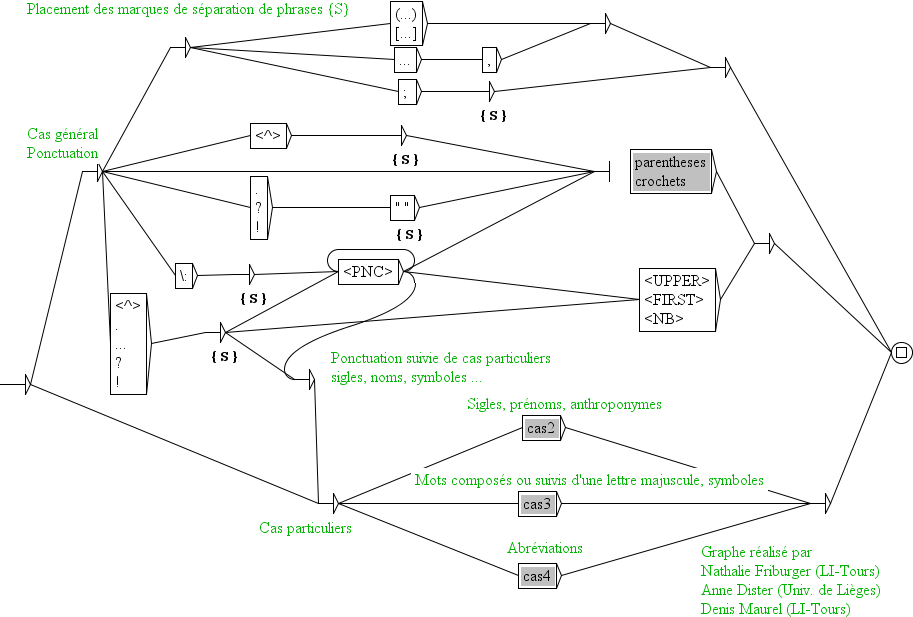
\includegraphics[width=15cm]{resources/img/fig2-10-Sentence.png}
\caption{Grammaire de découpage en phrases pour le français
\label{fig-example-sentence-splitting}}
\end{center}
\end{figure}

\noindent  Lorsqu’un chemin de la grammaire reconnaît une séquence dans le texte et que ce chemin
produit le symbole délimiteur de phrases \verb+{S}+\index{\verbt{\{S\}}}\index{Délimiteur de phrases},
on insère ce symbole dans le texte. Ainsi,
un chemin de la grammaire de la figure~\ref{fig-example-sentence-splitting} reconnaît la séquence
composée d’un point d’interrogation et d’un mot commençant par une majuscule et insère le symbole 
\verb+{S}+ entre le point d’interrogation et le mot suivant. Le texte suivant :


\bigskip
\textit{Quelle heure est-il ? Huit heures.}

\bigskip
\noindent deviendrait donc :

\bigskip
\textit{Quelle heure est-il ?\{S\} Huit heures.}

\bigskip
\noindent Une grammaire de découpage peut manipuler les symboles spéciaux, ou méta-symboles, suivants :

\index{\verbc{<E>}}\index{Epsilon|see{<E>}}
\index{\verbc{<MOT>}}\index{\verbc{<MIN>}}\index{\verbc{<MAJ>}}\index{\verbc{<PRE>}}\index{\verbc{<NB>}}
\index{\verbc{<PNC>}}\index{\verbc{<^>}}\index{\verbt{\#}}\index{\verbc{<WORD>}}\index{\verbc{<UPPER>}}\index{Méta-symboles}
\index{\verbc{<LOWER>}}\index{\verbc{<FIRST>}}
\begin{itemize}
  \item \verb+<E>+~: mot vide, ou epsilon. Reconnaît la séquence vide~;
  \item \verb+<WORD>+~: reconnaît n’importe quelle suite de lettres~;
  \item \verb+<LOWER>+~: reconnaît n’importe quelle suite de lettres minuscules~;
  \item \verb+<UPPER>+~: reconnaît n’importe quelle suite de lettres majuscules~;
  \item \verb+<FIRST>+~: reconnaît n’importe quelle suite de lettres commençant par une majuscule~;
  \item \verb+<NB>+~: reconnaît n’importe quelle suite de chiffres contigus (1234 est reconnu mais pas 1 234)~; 
  \item \verb+<PNC>+~: reconnaît les symboles de ponctuation ; , ! ? : ainsi que les points d’exclamation
  	  et d’interrogation inversés de l’espagnol et quelques signes de ponctuation asiatiques~;
  \item <\verb+^+>~: reconnaît un retour à la ligne~;
  \item \verb+#+~: interdit la présence de l’espace.
\end{itemize}

\noindent  Les anciens codes correspondant à \verb+<WORD>+, \verb+<LOWER>+, \verb+<UPPER>+ et \verb+<FIRST>+
 étaient respectivement \verb+<MOT>+, \verb+<MIN>+, \verb+<MAJ>+ et \verb+<PRE>+.
 Ils restent opérationnels afin de conserver la compatibilité descendante
 du système avec les graphes existants. Même s'il n'est pas prévu de supprimer ces codes, on recommande de les éviter dans les graphes conçus pour fonctionner avec les versions plus récentes\footnote{À partir de la version 3.1bêta, révision 4072 du 2 octobre 2015.},
pour ne pas faire augmenter inutilement le nombre de masques lexicaux en usage.

\bigskip
\noindent Par défaut, l’espace est facultatif entre deux boîtes. Si l’on veut interdire la présence
de ce séparateur, il faut utiliser le symbole spécial \verb+#+. À l’inverse, si vous souhaitez
forcer la présence de l’espace, vous devez utiliser la séquence \verb+" "+. Les lettres minuscules
et majuscules sont définies par un fichier alphabet\index{Fichier!alphabet}\index{Alphabet}
(voir chapitre~\ref{chap-file-formats}). Pour plus de détails sur les graphes,
voir le chapitre~\ref{chap-grammars}. Pour plus de détails sur le découpage d’un texte en phrases,
voir \cite{ameliorer-decoupage-en-phrases}. La grammaire utilisée se nomme \verb+Sentence.fst2+ et
se trouve dans le répertoire suivant~:\index{Fichier!\verbc{Sentence.fst2}}

\bigskip
\verb+/(répertoire personnel)/(langue)/Graphs/Preprocessing/Sentence+

\bigskip
\noindent L’application de cette grammaire à un texte s’effectue grâce au programme \verb+Fst2Txt+
\index{\verbc{Fst2Txt}}\index{Programmes externes!\verbc{Fst2Txt}} en mode MERGE.\index{MERGE} 
Cela signifie que les sorties produites par la grammaire, en l’occurrence le symbole \verb+{S}+,
sont insérées dans le texte. Ce programme prend en entrée un fichier \verb+.snt+ et le modifie.


\subsection{Normalisation de formes non ambiguës}
\index{Normalisation!de formes non ambiguës}
\index{Grammaires!normalisation!de formes non ambiguës}

Certaines formes présentes dans les textes peuvent être normalisées (par exemple, la séquence
française "\textit{l'on}" est équivalente à la forme "\textit{on}"). Chaque utilisateur peut donc
vouloir effectuer des remplacements en fonction de ses besoins. Toutefois, il faut faire
attention à ce que les formes normalisées soient non ambiguës, ou à ce que la disparition de
l’ambiguïté soit sans conséquence pour l’application recherchée.


\bigskip
\noindent Si l’on décide de remplacer la forme "\textit{audit}" par "\textit{à le-dit}",
 la phrase :

\bigskip
\textit{La cour a procédé à un audit des comptes de cette société.}

\bigskip
\noindent sera remplacée par la phrase incorrecte :

\bigskip
\textit{La cour a procédé à un à le-dit des comptes de cette société.}

\bigskip
\noindent Il faut donc être très prudent lorsque l’on manipule la grammaire de normalisation.
Il faut également faire attention aux espaces.
En effet, si l’on remplace "\textit{c’}" par "\textit{ce}" non suivi par un espace, la phrase :


\bigskip
\textit{Est-ce que c’était toi ?}

\bigskip
\noindent sera remplacée par la séquence incorrecte :

\bigskip
\textit{Est-ce que ce était toi ?}

%\bigskip
%\noindent To avoid this problem, one should explicitly insert a space,
%\textit{i.e.} replace "\textit{'re}" by "\textit{ are}".

\bigskip
\noindent Les symboles acceptés par les grammaires de normalisation sont les mêmes que ceux
autorisés dans les grammaires de découpage en phrases. La grammaire utilisée se nomme
\verb+Replace.fst2+ et se trouve dans le répertoire suivant~:

\bigskip \verb+/(répertoire personnel)/(langue)/Graphs/Preprocessing/Replace+

\bigskip
\noindent Comme pour le découpage en phrases, cette grammaire est utilisée avec le programme
\verb+Fst2Txt+ \index{Programmes externes!\verbc{Fst2Txt}}\index{\verbc{Fst2Txt}}, mais cette fois en
mode REPLACE, ce qui signifie que les entrées reconnues par la grammaire sont remplacées par les
séquences produites par celle-ci. On peut voir sur la figure~\ref{fig-normalization-grammar} une
grammaire qui normalise des contractions verbales en anglais.

\begin{figure}[!p]
\begin{center}
\includegraphics[height=17cm,angle=90]{resources/img/fig2-11.pdf}
\caption{Grammaire de normalisation de formes verbales en anglais\label{fig-normalization-grammar}}
\end{center}
\end{figure}



\subsection{Découpage du texte en unités lexicales}
\index{Texte!découpage en unités lexicales}
\index{Découpage!en unités lexicales}
\index{Token}\index{Tokenisation}
\label{tokenization}
Certaines langues, en particulier les langues asiatiques, utilisent les séparateurs de façon
différente des langues occidentales ; les espaces peuvent être interdits, facultatifs ou
obligatoires. Pour pouvoir gérer ces particularités au mieux, Unitex découpe les textes d’une
manière dépendante de la langue. Ainsi, les langues comme le français sont traitées selon le
principe suivant :

\bigskip
\noindent Une unité lexicale peut être :
\begin{itemize}
  \item soit le délimiteur de phrases \verb+{S}+;
  \item le marqueur \verb+{STOP}+.\index{\verbt{\{STOP\}}} Contrairement au délimiteur de phrases
  \verb+{S}+, le marqueur \verb+{STOP}+ ne peut JAMAIS être reconnu par une grammaire, de quelque
  façon que ce soit. Il peut être utilisé dans un corpus pour délimiter des élements. Par exemple,
  si un corpus est formé de nouvelles séparées par \verb+{STOP}+, il est impossible pour une
  grammaire de reconnaître une séquence qui chevauche la fin d'une nouvelle et le début de la
  suivante;
  \item une étiquette lexicale \verb+{aujourd'hui,.ADV}+;
  \item une séquence de lettres contiguës (les lettres sont définies dans le fichier alphabet de la
  langue);
  \index{Fichier!alphabet}
  \item un (et un seul) caractère different d'une lettre, i.e. tous les caractères non définis
  dans le fichier alphabet de la langue courante; s'il s'agit d'une newline, il est remplacé par un
  espace.
\end{itemize}

\bigskip
\noindent Pour les autres langues, le découpage est effectué caractère par caractère, à l’exception
du délimiteur de phrases \verb+{S}+ le marqueur \verb+{STOP}+ et des étiquettes lexicales. Ce
découpage basique garantit le fonctionnement d’Unitex, mais limite l’optimisation des opérations de
recherche de motifs. Par exemple une boite contenant \verb+aujourd'hui+ ne reconnaitra pas l'étiquette lexicale \verb+{aujourd'hui,.ADV}+. Pour la reconnaitre, il faut placer dans la boite le masque lexical: \verb+<aujourd'hui>+.


\bigskip
\noindent Quel que soit le mode de découpage, les retours à la ligne présents
dans un texte sont remplacés par des espaces. Ce découpage est effectué par le programme
\verb+Tokenize+\index{\verbc{Tokenize}} \index{Programmes externes!\verbc{Tokenize}}.
Ce programme produit plusieurs fichiers, stockés dans le répertoire du texte~:
\begin{itemize}
  \item \verb+tokens.txt+ contient la liste des unités lexicales dans l’ordre où elles ont été
  	  trouvées dans le texte;\index{Fichier!\verbc{tokens.txt}}
  \item \verb+text.cod+  contient un tableau d’entiers; chaque entier correspondant à l’indice d’une
  	  unité lexicale dans le fichier \verb+tokens.txt+;
  \index{Fichier!\verbc{text.cod}}
  \item \verb+tok_by_freq.txt+ contient la liste des unités lexicales triée par ordre de fréquence;
  \index{Fichier!\verbc{tok_by_freq.txt}}
  \item \verb+tok_by_alph.txt+ contient la liste des unités lexicales triée par ordre alphabétique;
  \index{Fichier!\verbc{tok_by_alph.txt}}
\item \verb+stats.n+ contient quelques statistiques sur le texte. \index{Fichier!\verbc{stats.n}}
\end{itemize}

\bigskip
\noindent Le découpage du texte :

\bigskip
\textit{Un sou c’est un sou.}

\bigskip
\noindent donne la liste d’unités lexicales suivantes :  \textit{UN} ESPACE \textit{sou c ’ est un
.}

\bigskip
\noindent On peut remarquer qu’il est tenu compte de la casse (Un et un sont deux unités distinctes), mais que chaque unité n’est codée qu’une fois. En numérotant ces unités de 0 à 7,
ce texte peut être représenté par la séquence d’entiers décrite dans le tableau suivant :

\bigskip
\begin{table}[!ht]
\begin{center}
\begin{tabular}{|p{2.8cm}||c|c|c|c|c|c|c|c|c|c|c|c|}
\hline
Indice             & 0 & 1 & 2 & 1 & 3 & 1 & 4 & 1 & 2 & 5
\\
\hline
Unité lexicale correspondante & \textit{UN} &   & \textit{sou} &   & \textit{est} &  & \textit{UN}
& & \textit{sou} & \textit{.}
\\
\hline
\end{tabular}
\caption{Représentation du texte \textit{Un sou c’est un sou.}}
\end{center}
\end{table}

\bigskip
\noindent Pour plus de détails, voir le chapitre~\ref{chap-file-formats}.

\begin{figure}[!ht]
\begin{center}
\includegraphics[height=10cm]{resources/img/fig2-12.png}
\caption{Unités lexicales d’un texte anglais triées par fréquence}
\end{center}
\end{figure}



\subsection{Application de dictionnaires}
\label{text-applying-dictionaries}
\index{Dictionnaire!application}
\index{Ressources!lexicales|see{Dictionnaire}}
L’application de dictionnaires consiste à construire le sous-ensemble des dictionnaires
ne contenant que les formes présentes dans le texte. Ainsi, le résultat de l’application des
dictionnaires du français au texte \textit{Igor mange une pomme de terre} produit le dictionnaire de
mots simples suivant :
\index{Mots!simples}

\bigskip
\begin{verbatim}
de,.DET+z1
de,.PREP+z1
de,.XI+z1
mange,manger.V+z1:P1s:P3s:S1s:S3s:Y2s
pomme,.A+z1:ms:fs:mp:fp
pomme,.N+z1:fs
pomme,pommer.V+z3:P1s:P3s:S1s:S3s:Y2s
terre,.N+z1:fs
terre,terrer.V+z1:P1s:P3s:S1s:S3s:Y2s
une,.N+z1:fs
une,un.DET+z1:fs
\end{verbatim}

\bigskip
\noindent ainsi que le dictionnaire de mots composés contenant l’unique entrée
:\index{Mots!composés}

\bigskip
\begin{verbatim}
pomme de terre,.N+z1:fs
\end{verbatim}

\bigskip
\noindent La séquence \textit{Igor} n'étant ni un mot simple du français, ni une partie de mot
composé, a été considérée comme un mot inconnu.\index{Mots!inconnus} L’application de dictionnaires
s’effectue avec le programme \verb+Dico+.\index{\verbc{Dico}}\index{Programmes externes!\verbc{Dico}}
Les trois fichiers produits (\verb+dlf+ pour les mots simples, \verb+dlc+ pour les mots composés et
\verb+err+ pour les mots inconnus) sont placés dans le répertoire du texte. On appelle dictionnaires
du texte les fichiers \verb+dlf+ et \verb+dlc+
\index{Dictionnaire!du texte}
\index{Fichier!\verbc{dlf}}
\index{Fichier!\verbc{dlc}}\index{Fichier!\verbc{err}}

\bigskip
\noindent Une fois l’application des dictionnaires effectuée, Unitex présente par ordre alphabétique
les mots simples, composés et inconnus trouvés dans une fenêtre. La figure~\ref{fig-Dico-application-results} montre les résultats pour un texte anglais.

\begin{figure}[!ht]
\begin{center}
\includegraphics[width=12cm]{resources/img/fig2-13.png}
\caption{Résultats de l’application de dictionnaires sur un texte
anglais\label{fig-Dico-application-results}}
\end{center}
\end{figure}

\bigskip
\noindent Il est également possible d’appliquer des dictionnaires en dehors du prétraitement du
texte. Pour cela, il faut cliquer sur "Apply Lexical Resources..." dans le menu "Text". Unitex
affiche alors une fenêtre (voir figure ~\ref{fig-Dico-configuration}) qui permet de choisir la
liste des dictionnaires à appliquer.


\begin{figure}[!ht]
\begin{center}
\includegraphics[width=10cm]{resources/img/fig2-14.png}
\caption{Paramétrage de l’application des dictionnaires\label{fig-Dico-configuration}}
\end{center}
\end{figure}

\bigskip
\noindent La liste "User resources" recense tous les dictionnaires \verb+.bin+ et \verb+.fst2+
présents dans le répertoire \verb+(langue)/Dela+ de l’utilisateur. Les dictionnaires du système sont
listés dans le cadre intitulé "System resources". Utilisez <Ctrl+click> pour sélectionner plusieurs
dictionnaires. Les dictionnaires systèmes sont appliqués avant les dictionnaires utilisateurs.
Vous pouvez choisir l'ordre des dictionnaires des listes utililisateur et système à l'aide des
flèches haut et bas (voir figure \ref{fig-Dico-configuration}). Le bouton "Set Default" vous permet
de définir la sélection courante de dictionnaires comme sélection par défaut. Cette sélection par
défaut sera utilisée lors du prétraitement si vous choisissez l’option "Apply All default
Dictionaries".\index{Dictionnaire!sélection par défaut}
Si vous effectuez un clic droit au-dessus d’un nom de dictionnaire, la documentation du
dictionnaire, si elle existe, s’affichera dans le cadre inférieur.


\subsection{Analyse des mots composés libres en néerlandais, allemand, norvégien et russe}
\index{Norvégien!mots composés libres}
\index{Allemand!mots composés libres}
\index{Néerlandais!mots composés libres}
\index{Russe!mots composés libres}
\index{Analyse des mots composés libres!langues germaniques}
\index{Mots!composés libres!langues germaniques}
\index{Analyse des mots composés libres!russe}
\index{Mots!composés libres!russe}

\label{section-Norwegian-compound-words}
Dans certaines langues comme le norvégien, il est possible de former des mots composés
libres en soudant leurs éléments. Par exemple, le mot \textit{aftenblad} signifiant \textit{journal
du soir} est obtenu en combinant les mots \textit{aften} (\textit{soir}) et \textit{blad}
(\textit{journal}). Le programme \verb+PolyLex+ \index{\verbc{PolyLex}}\index{Programmes
externes!\verbc{PolyLex}} explore la liste des mots inconnus après application des dictionnaires au
texte et essaye d’analyser chacun de ces mots comme un mot composé. Si un mot possède au moins une
analyse, il est retiré de la liste des mots inconnus et les lignes de dictionnaires produites pour
ce mot sont ajoutées au dictionnaire des mots simples du texte.

\section{Ouverture d’un texte taggué}
Un texte taggué est un texte contenant des entrées lexicales entre accolades comme par
exemple :


\bigskip
\textit{I do not like the \{square bracket,.N\} sign! \{S\}}

\bigskip
\noindent De tels tags permettent de lever des ambiguïtés en interdisant tout autre interprétation.
Dans notre exemple, on ne pourra pas reconnaître square bracket comme combinaison de deux mots
simples.


\bigskip
\noindent Toutefois, la présence de ces tags peut perturber l’application des graphes de
prétraitement. L’utilisateur dispose donc de la commande "Open Tagged Text..." dans le menu "Text",
grâce à laquelle il peut ouvrir un texte contenant des tags sans que les graphes de prétraitements
ne soient appliqués, comme on le voit sur la figure \ref{preprocess-tagged-text}.

\bigskip
\begin{figure}[!ht]
\begin{center}
\includegraphics[width=14cm]{resources/img/fig2-15.png}
\caption{Prétraitement d’un texte taggué\label{preprocess-tagged-text}}
\end{center}
\end{figure}


\chapter{Dictionnaires}
\label{chap-dictionaries}

\section{Les dictionnaires DELA}
\index{DELA}\index{Dictionnaire!format}\index{LADL}

Les dictionnaires électroniques utilisés par Unitex utilisent le formalisme DELA (Dictionnaires
Electroniques du LADL). Ce formalisme permet de décrire les entrées lexicales simples et composées
\index{Entrée lexicale} d’une langue en leur associant de façon optionnelle des
informations grammaticales, sémantiques et flexionnelles. On distingue deux sortes de dictionnaires
électroniques. Le type que l’on utilise le plus couramment est le dictionnaire de formes fléchies,
appelé DELAF (DELA de formes Fléchies) ou encore DELACF (DELA de formes Composées
Fléchies) lorsqu’il s’agit d’un dictionnaire de mots composés.\index{DELAF|(}
\index{DELACF}\index{Dictionnaire!DELAF|(}\index{Dictionnaire!DELACF}
Le second type est le dictionnaire de formes non fléchies appelé DELAS (DELA de formes Simples)
ou DELAC (DELA de formes Composées).
\index{DELAS}\index{DELAC}\index{Dictionnaire!DELAS}\index{Dictionnaire!DELAC}
Les programmes d’Unitex ne font pas de distinction entre les dictionnaires de formes
simples et composées. Nous utiliserons donc les termes DELAF et DELAS pour désigner les deux sortes
de dictionnaires que leurs entrées soient simples, composées ou mixtes.

\subsection{Format des DELAF}
\label{section-DELAF-format}
\subsubsection{Syntaxe d’une entrée}
\label{section-DELAF-entry-syntax}
Une entrée d’un DELAF est une ligne de texte terminée par un retour à la ligne qui
respecte le schéma suivant :

\bigskip
\begin{verbatim}
mercantiles,mercantile.A+z1:mp:fp/ceci est un exemple
\end{verbatim}

\bigskip
\noindent Les différents éléments qui forment cette ligne sont les suivants:

\bigskip
\begin{itemize}
\item \verb+mercantiles + est la forme fléchie de l’entrée.\index{Forme!fléchie} Cette forme fléchie
est obligatoire;
  
\bigskip \item \verb+mercantile+ est la forme canonique (lemme) de l’entrée.
\index{Lemme}\index{Forme!canonique} Pour les noms et les adjectifs, il s’agit
en général de la forme au masculin singulier; pour les verbes, la forme canonique est
l’infinitif. Cette information peut être omise comme dans l’exemple suivant :

  
\bigskip
\verb$boîte à merveilles,.N+z1:fs$
  
\bigskip Cela signifie alors que la forme canonique est identique à la forme fléchie. La forme
canonique est séparée de la forme fléchie par une virgule;
\index{\verbc{,}}
  
\bigskip \item \verb$A+z1$ est la séquence d’informations grammaticales et sémantiques.
\index{Informations!grammaticales}\index{Informations!sémantiques} Dans notre exemple, \verb+A+
désigne un adjectif, et \verb+z1+ ndique qu’il s’agit d’un mot courant (voir tableau ~\ref{tab-semantic-codes}).

Toute entrée doit comporter au moins un code grammatical ou sémantique, séparé de
la forme canonique par un point. S’il y a plusieurs codes, ceux-ci doivent être séparés
par le caractère \verb$+$\index{\verbc{+}}\index{\verbc{.}}.
  
\bigskip
\item \verb+:mp:fp+ est la séquence d’informations flexionnelles.
\index{Informations!flexionnelles} Ces informations décrivent le genre, le nombre, les temps et modes
de conjugaisons, les déclinaisons pour les langues à cas, etc. Ces informations sont facultatives.
Un code flexionnel est composé d’un ou plusieurs caractères codant chacun une information. Les codes
flexionnels doivent être séparés par le caractère :. Dans notre exemple, \verb+m+ signifie masculin,
\verb+p+ pluriel et \verb+f+ féminin (voir tableau ~\ref{tab-inflectional-codes}). Le caractère \verb+:+ s’interprète comme un OU logique. Ainsi, \verb+:mp:fp+ signifie "masculin pluriel", ou "féminin pluriel". Comme chaque caractère correspond à une information, il est inutile d’utiliser plusieurs fois un même caractère. Ainsi, coder le participe passé avec le code\verb+:PP+ serait strictement équivalent à utiliser \verb+:P+ seul;\index{\verbc{:}}
  
\bigskip \item \verb+/ceci est un exemple+ est un commentaire. Les commentaires sont facultatifs et
doivent être introduits par le caractère \verb+/+. Les commentaires sont supprimés lorsque
l’on comprime les dictionnaires. \index{Commentaire!dans un dictionnaire} \index{Dictionnaire!commentaire}\index{\verbc{/}}
\end{itemize}

\bigskip
\noindent REMARQUE IMPORTANTE : il est possible d’utiliser le point et la virgule dans une
entrée de dictionnaire. Pour cela, il faut les déspécialiser avec le caractère
\verb+\+ \index{\verbt{\textbackslash,}}\index{\verbt{\textbackslash.}}\index{\verbt{\textbackslash~}}:

\bigskip
\begin{verbatim}
3\,1415,PI.NOMBRE
Organisation des Nations Unies,O\.N\.U\..SIGLE
\end{verbatim}


\bigskip
\noindent ATTENTION : chaque caractère est pris en compte dans une ligne de dictionnaire. Par
exemple, si vous introduisez des espaces, ceux-ci seront considérés comme faisant partie
intégrante des informations. Dans la ligne suivante :


\begin{verbatim}
gît,gésir.V+z1:P3s /voir ci-gît
\end{verbatim}

\bigskip \noindent l’espace qui précède le caractère \verb+/+ sera considéré comme faisant partie
d’un code flexionnel à 4 caractères composés de \verb+P+, \verb+3+, \verb+s+ et d’un espace.


\bigskip \noindent Il est possible d’insérer des lignes de commentaires dans un dictionnaire DELAF
ou DELAS, en faisant débuter la ligne par le caractère $/$. Exemple

\bigskip
\begin{verbatim}
/ L’entrée nominale pour ’par’ est un terme de golf
par,.N+z3:ms
\end{verbatim}


\subsubsection{Mots composés avec espace ou tiret}

\index{Mots!composés!avec espace ou tiret}\index{\verbc{=}}\index{\verbt{\textbackslash=}}

Certains mots composés comme \textit{grand-mère} peuvent s’écrire avec des espaces ou avec
des tirets. Pour éviter de devoir dédoubler toutes les entrées, il est possible d’utiliser 
le caractère \verb+=+ . Lors de la compression du dictionnaire, le programme \verb+Compress+
\index{Programmes externes!\verbc{Compress}}\index{\verbc{Compress}} vérifie pour chaque ligne
si la forme fléchie ou la forme canonique contient le caractère \verb+=+. Si c’est le cas, le
programme remplace l’entrée par deux entrées : une où le caractère = est remplacé par un espace,
et une où il est remplacé par un tiret. Ainsi, l’entrée suivante :


\bigskip \verb$grand=mères,grand=mère.N:fp$

\bigskip
\noindent est remplacée par les deux lignes suivantes:

\bigskip
\verb$grand mères,grand mère.N:fp$

\verb$grand-mères,grand-mère.N:fp$


\bigskip
\noindent NOTE : si vous souhaitez écrire une entrée contenant le caractère \verb+=+,
déspécialisez-le avec le caractère \verb+\+ comme dans l’exemple suivant :


\bigskip
\verb$E\=mc2,.FORMULE$\\


Cette opération de remplacement a lieu lors de la compression du dictionnaire. Une fois
le dictionnaire comprimé, les signes \verb+=+ déspécialisés sont remplacés par de simples \verb+=+.
Ainsi, si l’on comprime un dictionnaire contenant les lignes suivantes :


\begin{verbatim}
E=mc2,.FORMULE
grand=mère,.N:fs
\end{verbatim}

\noindent et que l’on applique ce dictionnaire au texte :\\

\verb$Ma grand-mère m’a expliqué la formule E=mc2.$


\bigskip \noindent on obtiendra les lignes suivantes dans le dictionnaire de mots composés du texte:


\begin{verbatim}
E=mc2,.FORMULE
grand-mère,.N:fs
\end{verbatim}


\subsubsection{Factorisation d’entrées}

Plusieurs entrées ayant les mêmes formes fléchie et canonique peuvent être regroupées
en une seule à condition qu’elle aient les mêmes codes grammaticaux et sémantiques. Cela
permet entre autres de regrouper des conjugaisons identiques pour un même verbe :


\bigskip
\begin{verbatim}
glace,glacer.V+z1:P1s:P3s:S1s:S3s:Y2s
\end{verbatim}

\bigskip 
\noindent Si les informations grammaticales et sémantiques diffèrent, il faut créer des entrées dis-
tinctes :


\bigskip
\begin{verbatim}
glace,.N+z1:fs
glace,glacer.V+z1:P1s:P3s:S1s:S3s:Y2s
\end{verbatim}

\bigskip 
\noindent Certaines entrées ayant les mêmes codes grammaticaux et sémantiques peuvent avoir
des sens différents, comme c’est le cas pour le mot \textit{poêle} qui désigne un appareil de
chauffage ou un voile au masculin et un instrument de cuisine au féminin. On peut donc distinguer
les entrées dans ce cas :


\bigskip
\noindent
\texttt{poêle,.N+z1:fs/ poêle à frire}

\noindent
\texttt{poêle,.N+z1:ms/ voile, linceul; appareil de chauffage}

\bigskip 
\noindent NOTE : dans la pratique, cette distinction n’a pas d’autre conséquence qu’une
augmentation du nombre d’entrées du dictionnaire. Les différents programmes qui composent Unitex
donneront exactement les mêmes résultats si l’on fusionne ces entrées en :

\bigskip
\noindent
\texttt{poêle,.N+z1:fs:ms}

\bigskip 
\noindent L’intérêt de cette distinction est donc laissé à l’appréciation des personnes qui
construisent des dictionnaires.


\index{DELAF|)}\index{Dictionnaire!DELAF|)}

\subsection{Format des DELAS}
\label{section-DELAS-format}
\index{DELAS}\index{Dictionnaire!DELAS}

Le format des DELAS est très similaire à celui des DELAF. La différence est qu’on ne
mentionne qu’une forme canonique suivie de codes grammaticaux et/ou sémantiques. La
forme canonique est séparée des différents codes par une virgule. Voici un exemple d’entrée :


\begin{verbatim}
cheval,N4+Anl
\end{verbatim}

\noindent Le premier code grammatical ou sémantique sera interprété par le programme de flexion
comme le nom de la grammaire à utiliser pour fléchir l’entrée. L’entrée de l’exemple cidessus
indique que le mot \textit{cheval} doit être fléchi avec une grammaire nommée \verb+N4+.
Il est possible d’ajouter des codes flexionnels aux entrées, mais la nature de l’opération de
flexion limite l’intérêt de cette possibilité. Pour plus de détails, voir plus loin dans ce chapitre
la section ~\ref{section-automatic-inflection}.


\subsection{Contenu des dictionnaires}
\index{Dictionnaire!contenu}\index{Dictionnaire!codes utilisés}

Les dictionnaires fournis avec Unitex contiennent des descriptions des mots simples et
composés. Ces descriptions indiquent la catégorie grammaticale de chaque entrée, ses 
éventuels codes de flexion, ainsi que des informations sémantiques diverses. Les tableaux 
suivants donnent un aperçu des différents codes utilisés dans les dictionnaires fournis avec
Unitex. Ces codes ont la même signification pour presque toutes les langues, même si certains
d’entre eux sont propres à certaines langues (\textit{i.e.} marque du neutre, etc.).

\begin{table}[!ht]
\index{\verbc{A}}\index{\verbc{ADV}}\index{\verbc{CONJC}}\index{\verbc{CONJS}}\index{\verbc{DET}}
\index{\verbc{INTJ}}\index{\verbc{N}}\index{\verbc{PREP}}\index{\verbc{PRO}}\index{\verbc{V}}
\begin{center}
\begin{tabular}{|c|l|l|}
\hline
\textbf{Code} & \textbf{Signification} & \textbf{Exemples} \\
\hline
\verb+A+ & adjectif & fabuleux, broken-down \\
\hline
\verb+ADV+ & adverbe & réellement, à la longue \\
\hline
\verb+CONJC+ & conjonction de coordination & mais\\
\hline
\verb+CONJS+ & conjonction de subordination & puisque, à moins que \\
\hline
\verb+DET+ & déterminant & ses, trente-six \\
\hline
\verb+INTJ+ & interjection & adieu, mille millions de mille sabords \\
\hline
\verb+N+ & nom & prairie, vie sociale\\
\hline
\verb+PREP+ & préposition & sans, à la lumière de \\
\hline
\verb+PRO+ & pronom & tu, elle-même \\
\hline
\verb+V+ & verbe & continuer, copier-coller\\
\hline
\end{tabular}
\caption{Codes grammaticaux usuels\label{tab-grammatical-codes}}
\end{center}
\end{table}
\vspace{-0.7cm}
\begin{table}[!ht]
\index{\verbc{z1}}\index{\verbc{z2}}\index{\verbc{z3}}\index{\verbc{Abst}}\index{\verbc{Anl}}\index{\verbc{AnlColl}}
\index{\verbc{Conc}}\index{\verbc{ConcColl}}\index{\verbc{Hum}}\index{\verbc{HumColl}}\index{\verbc{t}}\index{\verbc{i}}
\index{\verbc{en}}\index{\verbc{se}}\index{\verbc{ne}}
\begin{center}
\begin{tabular}{|c|l|l|}
\hline
\textbf{Code} & \textbf{Signification} & \textbf{Exemple} \\
\hline
\verb+z1+ & langage courant & blague \\
\hline
\verb+z2+ & langage spécialisé & sépulcre \\
\hline
\verb+z3+ & langage très spécialisé & houer \\
\hline
\verb+Abst+ & abstrait & bon goût \\
\hline
\verb+Anl+ & animal & cheval de race \\
\hline
\verb+AnlColl+ & animal collectif & troupeau \\
\hline
\verb+Conc+ & concret & abbaye \\
\hline
\verb+ConcColl+ & concret collectif & décombres \\
\hline
\verb+Hum+ & humain & diplomate \\
\hline
\verb+HumColl+ & humain collectif & vieille garde \\
\hline
\verb+t+ & verbe transitif & foudroyer \\
\hline
\verb+i+ & verbe intransitif & fraterniser \\
\hline
\verb+en+ & particule pré-verbale (PPV) obligatoire & en imposer \\
\hline
\verb+se+ & verbe pronominal & se marier \\
\hline
\verb+ne+ & verbe à négation obligatoire & ne pas cesser de \\
\hline
\end{tabular}
\caption{Quelques codes sémantiques\label{tab-semantic-codes}}
\end{center}
\end{table}

%\bigskip
\noindent NOTE : les descriptions des temps du tableau ~\ref{tab-inflectional-codes} correspondent
au français. Néanmoins, la plupart de ces définitions se retrouvent dans plusieurs langues
(infinitif, présent, participe passé, etc.).


\bigskip
\noindent Malgré une base commune à la plupart des langues, les dictionnaires contiennent des
particularités de codage propres à chaque langue. Ainsi, les codes de flexion variant
beaucoup d’une langue à une autre, n’ont pas été décrits ici. Pour une description exhaustive
de tous les codes utilisés dans un dictionnaire, nous vous recommandons de vous adresser
directement à l’auteur du dictionnaire.


\begin{table}[!ht]
\index{\verbc{m}}\index{\verbc{f}}\index{\verbc{n}}\index{\verbc{s}}\index{\verbc{p}}\index{\verbc{1}}
\index{\verbc{2}}\index{\verbc{3}}\index{\verbc{P}}\index{\verbc{I}}\index{\verbc{S}}\index{\verbc{T}}
\index{\verbc{Y}}\index{\verbc{C}}\index{\verbc{J}}\index{\verbc{W}}\index{\verbc{G}}\index{\verbc{K}}
\index{\verbc{F}}
\begin{center}
\begin{tabular}{|c|l|}
\hline
\textbf{Code} & \textbf{Signification} \\
\hline
\verb+m+ & masculin \\
\hline
\verb+f+ & féminin \\
\hline
\verb+n+ & neutre \\
\hline
\verb+s+ & singulier \\
\hline
\verb+p+ & pluriel \\
\hline
\verb+1+, \verb+2+, \verb+3+ & 1st, 2nd, 3rd personne\\
\hline
\verb+P+ & présent de l’indicatif \\
\hline
\verb+I+ & imparfait de l’indicatif  \\
\hline
\verb+S+ & présent du subjonctif\\
\hline
\verb+T+ & imparfait du subjonctif \\
\hline
\verb+Y+ & présent de l’impératif \\
\hline
\verb+C+ & présent du conditionnel\\
\hline
\verb+J+ & passé simple \\
\hline
\verb+W+ & infinitif \\
\hline
\verb+G+ & participe présent \\
\hline
\verb+K+ & participe passé \\
\hline
\verb+F+ & futur \\
\hline
\end{tabular}
\caption{Codes flexionnels usuels\label{tab-inflectional-codes}}
\end{center}
\end{table}


\bigskip
\noindent Les codes présentés ne sont absolument pas limitatifs. Chaque utilisateur peut introduire
ses propres codes, et créer ses propres dictionnaires. Par exemple, on pourrait dans un but
pédagogique introduire dans les dictionnaires anglais des marques indiquant les faux-amis
français :

\bigskip
\begin{verbatim}
bless,.V+faux-ami/bénir
cask,.N+faux-ami/tonneau
journey,.N+faux-ami/voyage
\end{verbatim}

Il est également possible d’utiliser les dictionnaires pour stocker des informations parti-
culières. Ainsi, on pourrait utiliser la forme fléchie d’une entrée pour décrire un sigle et la
forme canonique pour en donner la forme complète :

\bigskip
\begin{verbatim}
ADN,Acide DésoxyriboNucléique.SIGLE
LADL,Laboratoire d’Automatique Documentaire et Linguistique.SIGLE
SAV,Service Après-Vente.SIGLE
\end{verbatim}



%%%%%%%%%%%%%%%%%%%%%%%%%%%%%%%%%%%%%%%%%%%%%%%%%%%
\section{Recherche d'un mot dans un dictionnaire}
\index{Dictionnaire!recherche}\index{Dictionnaire!consultation}\index{Consultation d'un dictionnaire}\index{Recherche dans un dictionnaire}
\label{section-dictionary-lookup}
Vous pouvez rechercher un mot dans plusieurs dictionnaires de deux manières : 

\begin{figure}[!ht]
\begin{center}
\includegraphics[width=13cm]{resources/img/fig3-1.png}
\caption{Menu "DELA"}
\end{center}
\end{figure}

\bigskip
\noindent
Si vous avez ouvert un dictionnaire, la fenêtrre affichée contient un champ qui vous permet
d'effectuer une recherche. Si le mot apparaît dans le dictionnaire, le bouton "Find" surligne la
première entrée correspondante. Si plusieurs entrées correspondent, vous pouvez les parcourir en
cliquant sur les deux boutons en forme de flèche.

\begin{figure}[!ht]
\begin{center}
\includegraphics[width=7cm]{resources/img/fig3-2.png}
\caption{Recherche d'un mot dans un dictionnaire}
\end{center}
\end{figure}

\bigskip
\noindent
Vous pouvez aussi rechercher un mots dans plusieurs dictionnaires en cliquant sur le bouton "Lookup" du menu "DELA". Vous pouvez ensuite sélectionner les dictionnaires dans lesquels rechercher le mot que vous avez entré.

\begin{figure}[!ht]
\begin{center}
\includegraphics[width=7cm]{resources/img/fig3-3.png}
\caption{Recherche d'un mot dans plusieurs dictionnaires}
\end{center}
\end{figure}

\bigskip
\noindent

%%%%%%%%%%%%%%%%%%




\section{Vérification du format du dictionnaire}
\index{Dictionnaire!vérification} \index{Vérification du format d'un dictionnaire}
Lorsque les dictionnaires sont de taille importante, il devient fastidieux de les vérifier à
la main. Unitex contient le programme \verb+CheckDic+\index{Programmes externes!\verbc{CheckDic}}
\index{\verbc{CheckDic}} qui vérifie automatiquement les dictionnaires DELAF et DELAS.

\bigskip
\noindent Ce programme effectue une vérification de la syntaxe des entrées. Pour chaque entrée
mal formée, le programme affiche le numéro de ligne, le contenu de cette ligne et la nature
de l’erreur. Les résultats de l’analyse sont sauvés dans un fichier nommé
\verb+CHECK_DIC.TXT+\index{Fichier!\verbc{CHECK_DIC.TXT}} qui est affiché une fois la vérification
terminée. En plus des éventuels messages d’erreurs, ce fichier contient la liste de tous les
caractères utilisés dans les formes fléchies et canoniques, la liste des codes grammaticaux et
sémantiques,ainsi que la liste des codes flexionnels utilisés.
La liste des caractères permet de vérifier que les caractères présents dans le dictionnaire
sont cohérents avec ceux présents dans le fichier alphabet de la langue. Chaque caractère est
suivi par sa valeur en notation hexadécimale. Les listes de codes peuvent être utilisées pour
vérifier qu’il n’y a pas de faute de frappe dans les codes du dictionnaire.
\index{Fichier!alphabet}


\bigskip
\noindent Le programme \verb+CheckDic+ fonctionne avec des dictionnaires non comprimés, c’est-à-dire
sous forme de fichiers texte. La convention généralement appliquée est de donner l’extension
\verb+.dic+ \index{Fichier!\verbc{.dic}}. Pour vérifier le format d’un dictionnaire, il faut tout
d’abord l’ouvrir en cliquant sur "Open..." dans le menu "DELA".


\begin{figure}[!ht]
\begin{center}
\includegraphics[width=10cm]{resources/img/fig3-4.png}
\caption{Exemple de dictionnaire\label{fig-dictionary-example}}
\end{center}
\end{figure}

\noindent Chargeons le dictionnaire de la figure~\ref{fig-dictionary-example}.
Pour lancer la vérification automatique, cliquez sur "Check Format..." dans le menu "DELA".
la fenêtre de la figure ~\ref{fig-dictionary-checking} apparaît alors.
Cette fenêtre vous permet de choisir le type du dictionnaire que vous voulez vérifier. Les
résultats de la vérification du dictionnaire de la figure~\ref{fig-dictionary-example},
 sont présentés sur la figure~\ref{fig-dictionary-checking-results}.

\bigskip
\noindent La première erreur est due au fait que le programme n’ait pas trouvé de point.
Le seconde, au fait qu’il n’ait pas trouvé de virgule marquant la fin de la forme fléchie.
La troisième erreur indique que le programme n’a trouvé aucun code grammatical ou sémantique.




\begin{figure}[!ht]
\begin{center}
\includegraphics[width=7cm]{resources/img/fig3-5.png}
\caption{Vérification automatique d’un dictionnaire\label{fig-dictionary-checking}}
\end{center}
\end{figure}

\begin{figure}[!p]
\begin{center}
\includegraphics[height=19.4cm]{resources/img/fig3-6.png}
\caption{Résultats d’une vérification automatique\label{fig-dictionary-checking-results}}
\end{center}
\end{figure}


\section{Tri}
\index{Dictionnaire!tri}\index{Tri!d'un dictionnaire}

Unitex manipule les dictionnaires sans se soucier de l’ordre des entrées. Toutefois, pour
des raisons de présentation, il est souvent préférable de trier les dictionnaires. L’opération
de tri varie selon plusieurs critères, à commencer par la langue du texte à trier. Ainsi, le
tri d’un dictionnaire thaï s’effectue selon un ordre différent de l’ordre alphabétique, si bien
qu’Unitex utilise un mode de tri développé spécialement pour le thaï (voir chapitre
 \ref{chap-external-programs}).

\bigskip
\noindent Pour les langues européennes, le tri s’effectue généralement selon l’ordre
lexicographique, avec toutefois quelques variantes. En effet, certaines langues comme le français
considèrent certains caractères comme équivalents. Par exemple, la différence entre les caractères
\verb+e+ et \texttt{é} est ignorée lorsque l’on veut comparer les mots \verb+manger+ et
\texttt{mangés}, car les contextes \verb+r+ et \verb+s+ permettent de décider de l’ordre. La
distinction n’est faite que lorsque les contextes sont identiques, ce qui est le cas si l’on
compare \texttt{pêche} et \texttt{pèche}.

\bigskip \index{Alphabet!tri}
\noindent
Afin de prendre en compte ce phénomène, le programme de tri \verb+SortTxt+  
\index{\verbc{SortTxt}}\index{Programmes externes!\verbc{SortTxt}} utilise un fichier qui définit des
équivalences de caractères. \index{Équivalence de caractères}  Ce fichier s’appelle
\verb+Alphabet_sort.txt+ \index{Fichier!\verbc{Alphabet_sort.txt}} et se trouve dans le répertoire
de la langue courante de l’utilisateur. Voici les premières lignes du fichier utilisé par défaut
pour le français :


\bigskip
\begin{minipage}{\textwidth}
\noindent\texttt{AÀÂÄaàâä}

\noindent\texttt{Bb}

\noindent\texttt{CÇcç}

\noindent\texttt{Dd}

\noindent\texttt{EÉÈÊËeéèêë}
\end{minipage}

\bigskip
\noindent Les caractères présents sur une même ligne sont considérés comme équivalents quand
le contexte le permet. Lorsqu’il faut comparer deux caractères équivalents, on les compare
selon l’ordre dans lequel ils apparaissent de gauche à droite sur la ligne. On peut voir sur
l’extrait ci-dessus qu’on ne fait pas de différence entre minuscules et majuscules, et qu’on
ignore les accents ainsi que la cédille.


\bigskip
\noindent Pour trier un dictionnaire, ouvrez-le, puis cliquez sur "Sort Dictionary" dans le menu
"DELA". Par défaut, le programme cherche toujours à utiliser le fichier \verb+Alphabet_sort.txt+.
Si ce fichier est absent, le tri se fait selon l’indice des caractères dans le codage Unicode.
En modifiant ce fichier, vous pouvez définir vos propres préférences de tri.


\bigskip
\noindent Remarque : après l’application des dictionnaires sur un texte, les fichiers
\verb+dlf+, \verb+dlc+ et \verb+err+ sont automatiquement triés avec ce programme.
\index{Fichier!\verbc{dlf}} \index{Fichier!\verbc{dlc}}\index{Fichier!\verbc{err}}



\section{Flexion automatique}
\label{section-automatic-inflection}
\index{Flexion automatique}\index{Conjugaison}\index{Déclinaison}\index{Dictionnaire!flexion automatique}
\subsection{Flexion des mots simples}

Comme décrit dans la section~\ref{section-DELAS-format}, une ligne de DELAS se compose généralement
d’une forme canonique et d’une séquence de codes grammaticaux ou sémantiques :


\begin{verbatim}
aviatrix,N4+Hum
matrix,N4+Math
radix,N4
\end{verbatim}

\bigskip
\noindent Le premier code rencontré est interprété comme le nom de la grammaire à utiliser pour
fléchir la forme canonique. Il y a deux formes possibles :

\begin{itemize}
\item \verb+N4+: nom de la grammaire=\verb+N4.fst2+, codes grammaticaux=\verb+N+
	(le plus long préfixe uniquement composé de lettres)
  \item \verb+N(NC_XXX)+: nom de la grammaire=\verb+NC_XXX.fst2+, codes grammaticaux=\verb+N+
\end{itemize}

\bigskip
\noindent Ces grammaires de flexion\index{Grammaires!de flexion}\index{Graphe!de flexion}\index{Transducteur!de flexion}
seront automatiquement compilées si
besoin est. Dans l’exemple ci-dessus, toutes les entrées seront fléchies avec une grammaire nommée
\verb+N4+.

\bigskip
\noindent Pour lancer la flexion, cliquez sur "Inflect..." dans le menu "DELA". La fenêtre de la 
figure~\ref{fig-inflection-configuration} permet d’indiquer au programme de flexion le
répertoire dans lequel se trouvent les grammaires de flexion. Par défaut, le sous-répertoire
\verb+Inflection+ du répertoire de la langue courante est utilisé. On peut aussi spécifier quels
types de mots le dictionnaire est supposé contenir. Si une entrée non conforme est
rencontrée, un message d'erreur sera affiché.

\bigskip
\begin{figure}[!ht]
\begin{center}
\includegraphics[width=8cm]{resources/img/fig3-7.png}
\caption{Configuration de la flexion automatique\label{fig-inflection-configuration}}
\end{center}
\end{figure}

\bigskip
\begin{figure}[!ht]
\begin{center}
\includegraphics[width=4.5cm]{resources/img/fig3-8.png}
\caption{Grammaire de flexion
\texttt{N4}\label{fig-example-inflectional-grammar}}
\end{center}
\end{figure}

\bigskip
\noindent La figure~\ref{fig-example-inflectional-grammar} présente un exemple de grammaire de
flexion. Les chemins décrivent les suffixes à ajouter ou à retrancher pour obtenir la forme fléchie
à partir de la forme canonique, et les sorties (texte en gras sous les boîtes) donnent les codes
flexionnels à ajouter à l’entrée du dictionnaire.


\bigskip
\noindent Dans notre exemple, deux chemins sont possibles. Le premier ne modifie pas la forme
canonique et ajoute le code flexionnel \verb+:s+. Le second retranche une lettre grâce à l’opérateur 
\verb+L+, ajoute ensuite le suffixe \verb+ces+ et ajoute le code flexionnel \verb+:mp+.

Voici les opérateurs utilisables:

\begin{itemize}
\item \verb+L+ (left)\index{\verbc{L}}\index{Opérateur!\verbc{L}} enlève une lettre à l’entrée;
  	  
\item \verb+R+ (right)\index{\verbc{R}}\index{Opérateur!\verbc{R}}
             rétablit une lettre de l’entrée. En français, beaucoup de verbes du premier
  	  groupe se conjuguent au présent à la troisième personne du singulier en retirant le
  	  \verb+r+ de l’infinitif et en changeant la 4$\ieme$ lettre en partant de la fin en
  	  \texttt{è}: \verb+peler+ $\rightarrow$ \texttt{pèle},
  	  \verb+acheter+ $\rightarrow$ \texttt{achète}, \texttt{gérer}
  	  $\rightarrow$ \texttt{gère}, etc. Plutôt que d’écrire un suffixe de flexion
  	  pour chaque verbe (\texttt{LLLLèle}, \texttt{LLLLète} and
  	  \texttt{LLLLère}), on peut utiliser l’opérateur \verb+R+ pour n’en écrire qu’un seul :
  	  \texttt{LLLLèRR}.
  	  
\item \verb+C+ (copy)\index{\verbc{C}}\index{Opérateur!\verbc{C}}
             duplique une lettre de l’entrée, en décalant tout ce qui se trouve à sa droite.
  	  
Supposons par exemple que l’on souhaite générer automatiquement des adjectifs en
\verb+able+ à partir de noms. Dans des cas comme \verb+regrettable+ ou \verb+réquisitionnable+,
  on observe un doublement de la consonne finale du nom. Pour éviter d’écrire un
graphe de flexion pour chaque consonne finale possible, on peut utiliser l’opérateur
\verb+C+ afin de dupliquer la consonne finale, quelle qu’elle soit;
  
  \item \verb+D+ (delete)\index{\verbc{D}}\index{Opérateur!\verbc{D}}
             supprime une lettre de l’entrée, en décalant tout ce qui se trouve à sa  droite.
Si l’on souhaite par exemple fléchir le mot roumain \verb+european+ en \verb+europeni+, on utilisera
la séquence \verb+LDRi+. Le \verb+L+ positionnera le curseur sur la lettre \verb+a+, \verb+D+ va
supprimer le \verb+a+, en décalant le \verb+n+ sur la gauche, puis \verb+Ri+ va rétablir le \verb+n+
et ajouter un \verb+i+.

\item \verb+U+ (unaccent)\index{\verbc{U}}\index{Opérateur!\verbc{U}}
          enlève l'accent du caractère courant s'il en comporte un.
	Par exemple la séquence \verb+LLUx+ appliquée au mot
	\texttt{mangés} produit la forme fléchie \verb+mangex+, puisque \verb+U+
	à transformé le \texttt{é} en \verb+e+.

\item \verb+P+ (uppercase)\index{\verbc{P}}\index{Opérateur!\verbc{P}}
          met en majuscule la première lettre de la pile. Par exemple, la séquence
	\verb$Px$ transforme \verb$foo$ en \verb$Foox$.
  
\item \verb+W+ (lowercase)\index{\verbc{W}}\index{Opérateur!\verbc{W}}
          met en minuscule la première lettre de la pile.

\item \verb+<R=?>+ \index{\verbc{<R=?>}}\index{Opérateur!\verbc{<R=?>}}
          remplace la première lettre de la pile par la lettre \verb+?+.

\item \verb+<I=?>+ \index{\verbc{<I=?>}}\index{Opérateur!\verbc{<I=?>}}
          insère la lettre \verb+?+ avant la première lettre de la pile.

\item \verb+<X=n>+ \index{\verbc{<X=n>}}\index{Opérateur!\verbc{<X=n>}}
          supprime les $n$ premières lettres de la pile.
\end{itemize}

\noindent Il y a également deux opérateurs spéciaux pour le  Coréen:
\begin{itemize}\index{Jamo}\index{Hangul}
\item \verb+J+ \index{\verbc{J}}\index{Opérateur!\verbc{J}}
supprime une lettre Jamo. Si le caractère est un Hangul, ce caractère est d'abord
remplacé par sa séquence équivalente en alphabet Jamo, ensuite, la dernière lettre Jamo est
supprimée. Si le caractère n'est ni un Jamo, ni un Hangul, une erreur est produite.
\item \verb+.+ (latin dot)\index{\verbc{.}}\index{Opérateur!\verbc{.}}
           insère une limite de syllabe. Ceci a un effet de ford, si le haut de la
	pile contient des lettres Jamo, elles sont recombinées en Hangul.
\end{itemize}


\bigskip
\noindent Voici un exemple qui décrit la flexion de \verb+choose+ en \verb+chosen+
      grâce à la séquence d’opérateurs \verb+LLDRRn+ :
\begin{itemize}
  \item Étape 0: initialisation de la pile avec la forme canonique; on place le curseur après la
  	  dernière lettre:

\begin{center}
\begin{tabular}{|l|l|l|l|l|l|l|l}
\multicolumn{6}{l}{} & \multicolumn{2}{l}{$\downarrow$} \\
\hline
\verb+c+ & \verb+h+ & \verb+o+ & \verb+o+ & \verb+s+ & \verb+e+ & \verb+ + & \\
\hline
\end{tabular}
\end{center}

\bigskip
\item Étape 1: on décale le curseur vers la gauche:

\begin{center}
\texttt{\textbf{L}LDRRn}

\begin{tabular}{|l|l|l|l|l|l|l|l}
\multicolumn{5}{l}{} & \multicolumn{3}{l}{$\downarrow$} \\
\hline
\verb+c+ & \verb+h+ & \verb+o+ & \verb+o+ & \verb+s+ & \verb+e+ & \verb+ + & \\
\hline
\end{tabular}
\end{center}

\bigskip
\item Étape 2: on décale une seconde fois le curseur vers la gauche:

\begin{center}
\texttt{\textbf{LL}DRRn}

\begin{tabular}{|l|l|l|l|l|l|l|l}
\multicolumn{4}{l}{} & \multicolumn{4}{l}{$\downarrow$} \\
\hline
\verb+c+ & \verb+h+ & \verb+o+ & \verb+o+ & \verb+s+ & \verb+e+ & \verb+ + & \\
\hline
\end{tabular}
\end{center}

\bigskip \item Étape 3: on décale tout ce qui est à droite du curseur vers la gauche :

\begin{center}
\texttt{\textbf{LLD}RRn}

\begin{tabular}{|l|l|l|l|l|l|l|l}
\multicolumn{3}{l}{} & \multicolumn{5}{l}{$\downarrow$} \\
\hline
\verb+c+ & \verb+h+ & \verb+o+ & \verb+s+ & \verb+e+ & \verb+ + & \verb+ + & \\
\hline
\end{tabular}
\end{center}

\bigskip
\item Step 4: on décale le curseur vers la droite:

\begin{center}
\texttt{\textbf{LLDR}Rn}

\begin{tabular}{|l|l|l|l|l|l|l|l}
\multicolumn{4}{l}{} & \multicolumn{4}{l}{$\downarrow$} \\
\hline
\verb+c+ & \verb+h+ & \verb+o+ & \verb+s+ & \verb+e+ & \verb+ + & \verb+ + & \\
\hline
\end{tabular}
\end{center}

\bigskip
\item Step 5: on décale encore le curseur vers la droite:

\begin{center}
\texttt{\textbf{LLDRR}n}

\begin{tabular}{|l|l|l|l|l|l|l|l}
\multicolumn{5}{l}{} & \multicolumn{3}{l}{$\downarrow$} \\
\hline
\verb+c+ & \verb+h+ & \verb+o+ & \verb+s+ & \verb+e+ & \verb+ + & \verb+ + & \\
\hline
\end{tabular}
\end{center}

\bigskip
\item Step 6: on écrit un \verb+n+

\begin{center}
\texttt{\textbf{LLDRRn}}

\begin{tabular}{|l|l|l|l|l|l|l|l}
\multicolumn{6}{l}{} & \multicolumn{2}{l}{$\downarrow$} \\
\hline
\verb+c+ & \verb+h+ & \verb+o+ & \verb+s+ & \verb+e+ & \verb+n+ & \verb+ + & \\
\hline
\end{tabular}
\end{center}
\end{itemize}

\bigskip
\noindent Une fois la séquence d’opérateurs épuisée, on prend le contenu de la pile jusqu’avant le
curseur pour former la forme fléchie (ici \verb+chosen+).

\bigskip
\noindent Le programme de flexion \verb+Inflect+ explore tous les chemins de la grammaire de flexion
en engendrant toutes les formes fléchies possibles. Afin d’éviter de devoir remplacer les noms des
grammaires de flexion par de vrais codes grammaticaux dans le dictionnaire obtenu, le programme
remplace ces noms par leurs plus longs préfixes composés de lettres. Ainsi, \verb+N4+ est remplacé
par \verb+N+. En choisissant judicieusement les noms des grammaires de flexion, on peut donc
engendrer directement un dictionnaire prêt à l’emploi.

\bigskip
\noindent La figure \ref{fig-inflection-result} montre le dictionnaire obtenu après flexion du DELAS de notre exemple.

\bigskip
\begin{figure}[!ht]
\begin{center}
\includegraphics[width=9.5cm]{resources/img/fig3-9.png}
\caption{Résultat de la flexion automatique\label{fig-inflection-result}}
\end{center}
\end{figure}
\bigskip

\subsection{Opérateurs de flexion avancés}
\label{advanced-inflection-operators}
Dans certaines langues, le processus de flexion entraine une modification de la racine du mot.
Plusieurs opérateurs ont été développés pour faciliter ce type de traitement. Ils permettent de rechercher
et d'enlever un suffixe du mot \verb+W+ \`a fléchir. Cette opération peut
\^etre accompagnée de la mémorisation dans une variable (\$ ou \pounds) d'un facteur de ce suffixe.
Ces opérateurs peuvent prendre les formes suivantes~:

%\bigskip
\begin{itemize}
\item \verb+<X$Y>+~: On recherche à la fin du mot \verb+W+ le suffixe \verb+Y+.
	Puis, on recherche \`a partir de la position atteinte la {\bf plus proche} occurrence de \verb+X+
	qui précède strictement celle de \verb+Y+ . La variable \$ contient alors le {\bf plus court facteur}
	({\bf\$}hortest) de \verb+W+ strictement compris entre
	\verb+X+ et \verb+Y+ (\verb+W = U.X.$.Y+) \footnote{Le point représente ici l'opération de concaténation.}.
	L'opérateur \verb+<X$Y>+ retire \verb+X.$.Y+ de \verb+W+ et donne une valeur à \$. Une fois qu'il a été appliqué,
	la séquence qui reste dans la pile est \verb+U+, et la variable \$ peut être utilisée dans le reste du chemin.
\item \verb+<X£Y>+~: On recherche à la fin du mot \verb+W+ le suffixe \verb+Y+.
	Puis, on recherche \`a partir de la position atteinte l'occurrence de \verb+X+ la {\bf plus à gauche} qui
	précède strictement celle de \verb+Y+. La variable {\pounds} contient alors le {\bf plus long facteur}
	({\bf£}ongest) de \verb+W+ strictement compris entre \verb+X+ et \verb+Y+ (\verb+W = U.X.£.Y+).
\item \verb+<X>+~: Si aucune variable n'est présente, on recherche \verb+X+ comme suffixe de \verb+W+
	(\verb+W =U.X+).
\item \verb+<$Y>+: Si le facteur \verb+X+ est absent, le {\bf plus court facteur \verb+$+} est la première lettre
	qui précède strictement \verb+Y+ .
\item \verb+<£Y>+~: Si le facteur \verb+X+ est absent, le {\bf plus long facteur \verb+£+} est le préfixe de
	\verb+W+ tel que  \verb+W = £.Y+.
\end{itemize}

%\bigskip
\noindent
Pour illustrer l'utilisation des ces opérateurs, considérons le verbe {\it reprendre}~:

\bigskip
\begin{center}
\begin{tabular}{|l|l|l|l|}
\hline
Verbe     & Opérateur & Variable & Résultat\\
\hline
\hline
reprendre & <re> & & reprend\\
reprendre & <\$> & \$ = e & reprendr\\
reprendre & <{\pounds}> &{\pounds}= reprendre & $\varepsilon$ \\
reprendre & <re\$re> & \$ = nd & rep\\
reprendre & <re{\pounds}re> & {\pounds} = prend & \\
reprendre & <\$re> & \$ = d & repren\\
reprendre & <re\$> & \$ =  $\varepsilon$ & reprendre\\
reprendre & <{\pounds}re> & {\pounds} = reprend & $\varepsilon$\\
reprendre & <re{\pounds}> & {\pounds} = prendre & re\\
\hline
\end{tabular}
\end{center}

\bigskip
\noindent
Le programme MultiFlex permet d'utiliser dix variables de type \$ dont les noms sont \$, \$1..., \$9
et dix variables de type {\pounds} dont les noms sont {\pounds}, {\pounds}1..., {\pounds}9. De plus,
plusieurs variables de types différents peuvent \^etre utilisées au sein d'une m\^eme opération.
Ainsi l'opérateur <{\pounds}3re\$7re> appliqué au verbe {\it reprendre} donne {\pounds}3 = 
 rep et \$7 = \verb+nd+.

\bigskip
\noindent
Si l'on considère les verbes \verb+accélérer+, \verb+sécher+, la
deuxième personne du présent de l'indicatif peut \^etre générée par l'opération <é\$er>è\$es~:

\begin{center}
\begin{tabular}{lllllllll}
	\verb+accélérer+ & <é\$er> & $\rightarrow$ & accél & \$ = r & + & è\$es &  $\rightarrow$ & \verb+accélères+\\
	\verb+sécher+ & <é\$er> & $\rightarrow$ & s & \$ = ch & + & è\$es & $\rightarrow$ & \verb+sèches+\\
\end{tabular}
\end{center}

\noindent
On remarque que le facteur \verb+$+ conservé dans la forme fléchie est de longueur variable (\verb+r+, \verb+ch+). 
La flexion de \verb+accélérer+ et \verb+sécher+ ne peut se faire que par des opérateurs de pile
classiques \`a l'aide d'une opération commune. Deux opérations différentes (\verb+-4RèCes+, \verb+-5RèCes+) sont
nécessaires. Le graphe de la figure~\ref{fig-inflection-secher} permet de fléchir des verbes comme
\verb+accélérer+ et \verb+sécher+ au présent.

\begin{figure}[!ht]
\begin{center}
\includegraphics[width=7cm]{resources/img/fig3-Advanced_operators_with_Variables-V_secher.png}
\caption{Graphe de flexion pour des verbes comme {\it accélérer}, {\it sécher}
\label{fig-inflection-secher}}
\end{center}
\end{figure}

\newpage
\noindent
Voici les flexions obtenues pour les verbes \verb+accélérer+ et \verb+sécher+:

\begin{figure}[!ht]
\begin{center}
\includegraphics[width=5cm]{resources/img/fig3-flexion_secher.png}
\end{center}
\end{figure}

\bigskip
\noindent
Le redoublement de certaines lettres lors de la flexion peut s'effectuer avec l'opérateur \$.
Par exemple l'adject {\it tranquil} en anglais possède deux formes au comparatif et deux au
superlatf. Le graphe de la figure ~\ref{fig-inflection-tranquil} permet de les produire.

\bigskip
\begin{figure}[!ht]
\begin{center}
\includegraphics[width=5.5cm]{resources/img/fig3-Advanced_operators_with_Variables-A_tranquil.png}
\caption{Graphe de flexion pour des adjectifs anglais comme {\it tranquil}
\label{fig-inflection-tranquil}}
\end{center}
\end{figure}

\noindent Voici les flexions obtenues pour l'adjectif anglais \verb+tranquil+:

\bigskip
\begin{figure}[!ht]
\begin{center}
\includegraphics[width=5cm]{resources/img/fig3-flexion_tranquil.png}
\end{center}
\end{figure}

\noindent Dans certaines langues, certaines formes fléchies comporte un préfixe qui s'ajoute devant la racine.
C'est le cas lors de la formation du participe passé en allemand. L'utilisation conjointe des
opérateurs \verb+£+ et \verb+$+ permet de fléchir le verbe allemand \verb+sprechen+ (parler)
au présent et participe passé comme le montre le graphe de la figure~\ref{fig-inflection-sprechen}.

\newpage
\begin{figure}[!htbp]
\begin{center}
\includegraphics[width=5cm]{resources/img/fig3-Advanced_operators_with_Variables-V_sprechen.png}
\caption{Graphe de flexion pour des verbes comme {\it sprechen}
\label{fig-inflection-sprechen}}
\end{center}
\end{figure}

\noindent Voici les flexions obtenues pour le verbe allemand \verb+sprechen+:

\bigskip
\begin{figure}[!ht]
\begin{center}
\includegraphics[width=5cm]{resources/img/fig3-flexion_sprechen.png}
\end{center}
\end{figure}

\noindent Si l'on veut fléchir le verbe à particule aussprechen on peut utiliser deux variables de type \$.
Le figure ~\ref{fig-inflection-aussprechen} montre un graphe qui comport les variables \verb+$1+ et \verb+$2+.

\bigskip
\begin{figure}[!ht]
\begin{center}
\includegraphics[width=10.5cm]{resources/img/fig3-Advanced_operators_with_Variables-V_aussprechen.png}
\caption{Graphe de flexion pour des verbes comme {\it aussprechen}
\label{fig-inflection-aussprechen}}
\end{center}
\end{figure}

\noindent Voici les flexions obtenues pour le verbe allemand \verb+aussprechen+:
\bigskip
\begin{figure}[!ht]
\begin{center}
\includegraphics[width=5cm]{resources/img/fig3-flexion_aussprechen2.png}
\end{center}
\end{figure}

\bigskip
\noindent \textbf{Codes sémantiques}
\noindent Dans certaines langues, il existe des caractéristiques flexionnelles qui correspondent
en fait à des caractéristiques sémantiques comme par exemple les marqueurs de la forme passive.
Ces codes peuvent ne pas apparaître comme des codes flexionnels, mais plutôt comme des codes
sémantiques. Pour produire des codes sémantiques, il faut insérer un signe plus au début de la
sortie d'une boîte. Cette boîte doit seulement contenir le code sémantique précédé d'un plus, comme
le montre la figure~\ref{fig-inflection-sem}.

\bigskip
\begin{figure}[!ht]
\begin{center}
\includegraphics[width=6cm]{resources/img/fig3-9sem.png}
\caption{Une grammaire de flexion avec un code sémantique\label{fig-inflection-sem}}
\end{center}
\end{figure}


\subsection{Flexion des mots composés}
Voir chapitre \ref{chap-multiflex}.


\subsection{Flexion des langues sémitiques}
\label{subsection-semitic-inflection}
\index{Langues sémitiques}
Les langues  sémitiques comme l'arabe ou l'hébreu se fléchissent d'une manière qui n'est pas facilement représentable
avec les opérateurs de flexion décrits ci-dessus. Leur morphologie obéit à une logique différente~:
les mots se fléchissent selon un \textit{squelette consonantique}\index{Squelette consonantique}.
Le processus de flexion combine ce squelette avec des voyelles.
Des opérateurs spécifiques ont été implémentés pour les langues sémitiques, et certains pourraient être utiles
aussi pour des langues en dehors de la famille sémitique, comme le tagalog.

\bigskip
\noindent Tout d'abord, voyons un cas où on ne code que les consonnes dans le champ lemme de l'entrée DELAS~:

\bigskip
\noindent \verb+ktb,$V31-123+

\bigskip
\noindent Le signe \verb+$+ avant le code grammatical indique que la grammaire de flexion est en mode sémitique, et
la forme \verb+ktb+ qui figure dans le champ lemme est le squelette consonantique. La figure \ref{semitic-grammar}
montre une grammaire jouet \verb+V31-123.grf+ qui illustre le fonctionnement du mode sémitique. Les grammaires
de flexion utilisent la translittération Buckwalter++ de l'écriture arabe (cf.~section~\ref{transliteration-Arabic}).

\bigskip
\begin{figure}[!ht]
\begin{center}
\includegraphics[width=10cm]{resources/img/fig3-15.png}
\caption{Une grammaire de flexion jouet en mode sémitique\label{semitic-grammar}}
\end{center}
\end{figure}

\noindent Le mode sémitique obéit aux règles suivantes:
\begin{enumerate}
\item Tous les opérateurs de flexion standard peuvent être utilisés (\verb+L+, \verb+R+, etc.).
\item Un chiffre représente une lettre du champ lemme (\verb+1+ pour la première,
\verb+2+ pour la seconde, etc). Dans notre exemple, \verb+1+, \verb+2+ et \verb+3+ représentent
respectivement \verb+k+, \verb+t+ et \verb+b+. Si on veut désigner une lettre après la neuvième,
on doit protéger son numéro avec des chevrons~: \verb+<10>+.
\end{enumerate}  

\noindent Le DELAF produit par cette grammaire est:\\ 
  
\verb+yakotubu,ktb.V:aI3ms+

\bigskip
\noindent Si on ne code que les consonnes dans le champ lemme et que deux entrées ont les mêmes
consonnes mais diffèrent par leurs voyelles, on doit coder les voyelles dans les grammaires de flexion~:\\ 

\verb+Hsb,$V3au	// compter, Hasaba, yaHosubu+

\verb+Hsb,$V3ii	// penser, Hasiba, yaHosibu+

\begin{figure}[!ht]
\begin{center}
\includegraphics[width=10cm]{resources/img/fig3-LEMMA-operator.png}
\caption{Une grammaire de flexion en mode sémitique avec l'opérateur <LEMMA>\label{LEMMA-operator}}
\end{center}
\end{figure}

\bigskip
\noindent Pour copier tout le champ lemme, on peut utiliser l'opérateur <LEMMA>.
Une boite contenant cet opérateur récupère tout le champ lemme mais ne dépend pas du nombre de lettres.
Cet opérateur est utile pour les noms et adjectifs arabes pour lesquels les formes du masculin sont obtenues en
insérant des voyelles dans le squelette consonantique, alors que celles du féminin le sont en ajoutant des
suffixes (figure~\ref{LEMMA-operator}). Dans cet exemple, on a codé à la fois les consonnes et les voyelles
dans le champ lemme.

\bigskip
\noindent L'opérateur <n.LEMMA>  copie le lemme depuis la $n$ième position jusqu'à la fin.
Par exemple, dans certains noms arabes, la voyelle brève de la première syllabe alterne~:
\verb+a/u+, \verb+a/i+ ou \verb+u/i+, comme dans \verb+nufaAyap+/\verb+nifaAyap+ ''ordures''.
La grammaire de flexion de la fig.~\ref{n.LEMMA-operator} produit à la fois les variantes en \verb+u+ et en  \verb+i+
comme formes fléchies de \verb+nufaAyap+.

\begin{figure}[!ht]
\begin{center}
\includegraphics[width=14cm]{resources/img/N0_i_0ap-f-At.png}
\caption{Une grammaire de flexion en mode sémitique avec l'opérateur <n.LEMMA>\label{n.LEMMA-operator}}
\end{center}
\end{figure}

\bigskip
\noindent En tagalog, une langue austronésienne parlée aux Philippines et qui utilise communément des infixes
et des redoublements pour la flexion, <LEMMA> et <n.LEMMA> peuvent être utiles pour produire des temps verbaux.
La grammaire de flexion jouet de la fig.~\ref{tagalog} produit le parfait \verb+kumain+, le futur \verb+kakain+
et l'imparfait \verb+kumakain+ du verbe \verb+kain+ ''manger''.

\begin{figure}[!ht]
\begin{center}
\includegraphics[width=12cm]{resources/img/V1um.png}
\caption{Une grammaire de flexion jouet pour le tagalog en mode sémitique\label{tagalog}}
\end{center}
\end{figure}

\section{Translittération des dictionnaires d'arabe}
\index{Translittération!arabe}\index{Dictionnaires!translittération}

Quand les linguistes arabes analysent des dictionnaires pour y détecter des erreurs,
la lecture dans l'écriture arabe est simple et efficace. Cependant, quand ils
créent des grammaires de flexion (section~\ref{section-automatic-inflection}), des éléments
de mots arabes apparaissent dans la même boite que des informations morpho-syntaxiques
codées dans l'alphabet latin, et dans ce contexte, les allers-retours entre l'écriture arabe,
qui se lit de droite à gauche, et l'alphabet latin, qui se lit de gauche à droite, ne sont pas
pratiques. Avec Unitex, on peut coder des grammaires de flexion entièrement dans l'alphabet
latin, en utilisant la translittération Buckwalter++,\index{Buckwalter++} une correspondance
biunivoque entre un codage Unicode de l'écriture arabe et des lettres de l'alphabet latin
(cf.~\cite{neme2011}, section~3.2, pp.~4--6). La translittération Buckwalter++ est définie
par la table des figures~\ref{buckwalter1} et \ref{buckwalter2}.
Unitex offre une fonctionnalité de translittération de dictionnaires DELAS et DELAF de l'arabe
vers le code Buckwalter++ et inversement (fig.~\ref{Arabic-transliteration}). Cette fonctionnalité
est accessible par le menu DELA.

\begin{figure}[!p]
\begin{center}
\includegraphics[height=23.5cm]{resources/img/buckwalter1-fr.pdf}
\caption{Table de translittération Buckwalter++, première moitié\label{buckwalter1}}
\end{center}
\end{figure}

\begin{figure}[!p]
\begin{center}
\includegraphics[height=23.5cm]{resources/img/buckwalter2-fr.pdf}
\caption{Table de translittération Buckwalter++, deuxième moitié\label{buckwalter2}}
\end{center}
\end{figure}

\begin{figure}[!ht]
\begin{center}
\includegraphics[width=15cm]{resources/img/Arabic-transliteration.pdf}
\caption{Translittération d'un dictionnaire DELAF
depuis le code Buckwalter++ (à gauche) vers l'écriture arabe (à droite)\label{Arabic-transliteration}}
\end{center}
\end{figure}


\section{Compression}
\index{Dictionnaire!compression}

Unitex applique aux textes des dictionnaires comprimés. La compression permet de réduire
la taille des dictionnaires et d’en accélérer la consultation. Cette opération s’effectue
avec le programme \verb+Compress+. \index{\verbc{Compress}}\index{Programmes externes!\verbc{Compress}}
Celui-ci prend en entrée un dictionnaire sous forme de fichier texte (par exemple
	\verb+mon_dico.dic+) et produit deux fichiers:\index{Fichier!\verbc{.dic}}

\begin{itemize}
  \item \verb+mon_dico.bin+ contient l’automate minimal des formes fléchies du dictionnaire;
  	  \index{Fichier!\verbc{.bin}}
  \item \verb+mon_dico.inf+ \index{Fichier!\verbc{.inf}}contient des codes qui permettent de
  	  reconstruire le dictionnaire d’origine à partir
  	  des formes fléchies contenues dans \verb+mon_dico.bin+.
\end{itemize}

\index{Automate!minimal}
\noindent L’automate minimal contenu dans \verb+mon_dico.bin+ est une représentation des formes
fléchies où tous les préfixes et suffixes
communs sont factorisés. Par exemple, l’automate minimal des mots \verb+me+, \verb+te+, \verb+se+,
\verb+ma+, \verb+ta+ et \verb+sa+
peut être représenté par le graphe de la figure~\ref{fig-example-minimal-automaton}.
\bigskip \begin{figure}[!ht]
\begin{center}
\includegraphics[width=5cm]{resources/img/fig3-10.png}
\caption{Représentation d’un exemple d’automate minimal\label{fig-example-minimal-automaton}}
\end{center}
\end{figure}

\noindent    Pour comprimer un dictionnaire, ouvrez-le puis cliquez sur "Compress into FST" dans le
menu "DELA". La compression est indépendante de la langue et du contenu du dictionnaire.
Les messages produits par le programme sont affichés dans une fenêtre qui ne se ferme pas
automatiquement. Vous pouvez ainsi voir la taille du fichier
\verb+.bin+, obtenu, le nombre de lignes lues ainsi que le nombre de codes flexionnels produits. La
figure ~\ref{fig-compression-result}
montre le résultat de la compression d’un dictionnaire de mots simples.

\bigskip
\begin{figure}[!ht]
\begin{center}
\includegraphics[width=14cm]{resources/img/fig3-11.png}
\caption{Résultat d’une compression\label{fig-compression-result}}
\end{center}
\end{figure}

\bigskip
\noindent À titre indicatif, les taux de compression généralement observés sont d’environ 95\% pour
les dictionnaires de mots simples et 50\% pour ceux de mots composés.


\bigskip
\noindent Quand le mode sémitique (\ref{subsection-semitic-inflection}) a beaucoup été utilisé lors de la flexion
d'un dictionnaire, une variante spécifique de l'algorithme de compression peut réduire la taille des fichiers
\verb+.bin+ et \verb+.inf+. Pour l'invoquer, soit on déclare la langue comme étant sémitique dans les préférences
globales, en cochant l'option ''Semitic language'' dans ''Preferences > Language and Presentation'', soit on
lance le programme Compress en ligne de commande avec l'option \verb+--semitic+.


\section{Application de dictionnaires}
\label{section-applying-dictionaries}
\index{Dictionnaire!application}

\bigskip
\noindent Unitex peut manipuler soit des dictionnaires compressés (\verb+.bin+) soit des graphes-dictionnaires (\verb+.fst2+). Ces dictionnaires peuvent être appliqués soit lors du prétraitement,
soit explicitement en cliquant sur "Apply Lexical Resources..." dans le menu "Text". Nous allons
maintenant détailler les règles de l’application des dictionnaires. Le cas des graphes-dictionnaires
sera abordé dans la section ~\ref{section-dictionary-graphs}.

\subsection{Priorités}
\label{section-dictionary-priorities}
\index{Dictionnaire!priorité}\index{Priorité!entre dictionnaires}
La règle de priorité est la suivante : si un mot du texte a été trouvé dans un dictionnaire,
ce mot ne sera plus pris en compte lors de l’application de dictionnaires ayant une priorité
inférieure.


\bigskip
\noindent Cela permet d’éliminer certaines ambiguïtés lors de l’application des dictionnaires.
Par exemple, le mot \textit{par} a une interprétation nominale dans le domaine du golf. Si l’on ne
veut pas envisager cet emploi, il suffit de créer un dictionnnaire filtre ne contenant que l’entrée 
\verb$par,.PREP$ et de le sauver en lui donnant la priorité la plus haute. De cette manière, même
si le dictionnaire des mots simples contient l’autre entrée, celle-ci sera ignorée grâce au jeu
des priorités.

\index{Dictionnaire!filtre}

\bigskip
\noindent Il y a trois niveaux de priorités. Les dictionnaires dont les noms sans extension se
terminent par \verb+-+\index{\verbc{-}}\index{\verbc{+}} ont la priorité la plus grande ; ceux dont
le nom se termine par \verb-+- ont la priorité la plus faible ; les autres dictionnaires sont
appliqués avec une priorité moyenne. L’ordre d’application de plusieurs dictionnaires ayant la même
priorité est sans importance. En ligne de commande, l’instruction :


\bigskip
\noindent
\verb$Dico ex.snt alph.txt ctr+.bin cities-.bin rivers.bin regions-.bin$

\bigskip \noindent appliquerait donc les dictionnaires dans l’ordre suivant (\verb+ex.snt+ est le
texte auquel sont appliqués les dictionnaires, \verb+alph.txt+ est le fichier alphabet utilisé):

\begin{enumerate}
  \item \verb$cities-.bin$
  \item \verb$regions-.bin$
  \item \verb$rivers.bin$
  \item \verb$ctr+.bin$
\end{enumerate}

\subsection{Règles d’application des dictionnaires}
\label{section-transducer-application-rules}

Outre la règle de priorités, l’application des dictionnaires s’effectue en respectant les
majuscules et les espaces. La règle du respect des majucules est la suivante :

\index{Règles!majuscules et minuscules}

\begin{itemize}
  \item s’il y a une majuscule dans le dictionnaire, alors il doit y avoir une majuscule dans le
texte ;

  \item s’il y a une minuscule dans le dictionnaire, il peut y avoir soit une minuscule soit une
majuscule dans le texte.

\end{itemize}

\noindent Ainsi, l’entrée \verb$pierre,.N:fs$ reconnaîtra les mots \verb+pierre+,
\verb+Pierre+ et \verb+PIERRE+, alors que

\noindent \verb$Pierre,.N+Prénom$ ne reconnaîtra que \verb+Pierre+ et \verb+PIERRE+. Les lettres
minuscules et majuscules sont définies par le fichier alphabet passé en paramètre au programme
\verb+Dico+\index{\verbc{Dico}}\index{Programmes externes!\verbc{Dico}}
\index{Fichier!\verbc{Alphabet.txt}}\index{Fichier!alphabet}\index{Alphabet}.\index{Règles!espace}

\bigskip
\noindent Le respect des espacements est une règle très simple : pour qu’une séquence du texte
soit reconnue par une entrée de dictionnaire, elle doit avoir exactement les mêmes espaces.
Par exemple, si le dictionnaire contient \verb+aujourd'hui,.ADV+, la séquence \verb+Aujourd' hui+
ne sera pas reconnue à cause de l’espace qui suit l’apostrophe.


\subsection{Graphes-dictionnaires}
\label{section-dictionary-graphs}\index{Graphe!dictionnaire}\index{Graphe-dictionnaire}
Le programme \verb+Dico+\index{\verbc{Dico}}\index{Programmes externes!\verbc{Dico}} est également capable
d’appliquer des graphes-dictionnaires.
Un graphe-dictionnaire est un graphe qui sert de dictionnaire.
Les graphes-dictionnaires respectent,
par défaut\footnote{Les graphes-dictionnaires morphologiques sont une exception
(section~\ref{section-morphological-dictionary-graphs}) .}, la règle suivante :
si on les applique avec le programme \verb+Locate+\index{\verbc{Locate}}\index{Programmes externes!\verbc{Locate}} en mode MERGE,\index{MERGE} ils doivent produire des séquences
correspondant à des lignes de DELAF.\index{DELAF}\index{Dictionnaire!DELAF}
Quand on les applique à un texte, ils attachent les étiquettes lexicales DELAF à ces séquences.


\begin{figure}[!p]
\begin{center}
\includegraphics[height=24cm]{resources/img/fig3-12.png}
\caption{Graphe-dictionnaire des éléments chimiques\label{elements}}
\end{center}
\end{figure}

\bigskip
\noindent La figure \ref{elements} montre un graphe reconnaissant les symboles chimiques. On peut
voir sur cette figure un premier avantage par rapport aux dictionnaires compressés : l’utilisation
des guillemets permet de forcer le respect de la casse. Ainsi, ce graphe reconnaîtra bien \verb+Fe+
mais pas \verb+FE+, alors qu’il est impossible de spécifier une telle interdiction dans un DELAF
usuel.

\bigskip
\noindent Pour faire un graphe-dictionaire, on utilise les outils pour les graphes (menu FSGraph, section~\ref{section-editing-graphs})
mais on les sauvegarde et on les compile de préférence dans le répertoire pour les dictionnaires (le répertoire Dela).
Pour appliquer un graphe-dictionnaire à un texte, on utilise un outil pour les dictionnaires: "Text > Apply lexical resources" (section~\ref{text-applying-dictionaries}).
\bigskip

\noindent Un autre avantage des graphes-dictionnaires est qu’ils peuvent exploiter les résultats
fournis par les dictionnaires appliqués précédemment. Ainsi, on peut appliquer le dictionnaire
général, puis étiqueter comme noms propres les mots inconnus commençant par une majuscule à l’aide
du graphe \verb$NPr+$ de la figure~\ref{graph-NPr}. Le \verb$+$ dans le nom du graphe lui donne une
priorité basse afin qu’il soit appliqué après le dictionnaire général. Pour fonctionner, ce graphe
se base sur les mots qui sont toujours inconnus après le passage du dictionnaire général. Les
crochets correspondent à une définition de contexte (voir la section \ref{section-contexts}).

\begin{figure}[!ht]
\begin{center}
\includegraphics[width=10.5cm]{resources/img/fig3-13.png}
\caption{Graphe-dictionnaire étiquetant comme noms propres les mots inconnus commençant par une
majuscule
\label{graph-NPr}}
\end{center}
\end{figure}

\bigskip
\noindent Comme les graphes-dictionnaires sont appliqués par le moteur du programme \verb+Locate+,
ils peuvent utiliser tout ce que le programme \verb+Locate+ autorise. En particulier, il est
possible d’utiliser les filtres morphologiques\index{Filtre morphologique} (section~\ref{section-filters}) et le mode morphologique (section~\ref{section-morphological-mode}).\index{Mode
morphologique}
Ainsi, le graphe de la figure \ref{graph-CR} utilise ces filtres pour reconnaître les nombres en
chiffres romains. Notons qu’il utilise également des contextes afin d’éviter, par exemple, que
\verb+C+ ne soit pris comme chiffre romain quand il est suivi par une apostrophe.

\begin{figure}[!p]
\begin{center}
\includegraphics[height=24cm]{resources/img/fig3-14.png}
\caption{Graphe-dictionnaire reconnaissant les nombres en chiffres romains\label{graph-CR}}
\end{center}
\end{figure}

\bigskip
\noindent Par défaut, les graphes-dictionnaires sont appliqués en mode MERGE. Il est possible 
de les appliquer en mode REPLACE, en ajoutant à leur le nom le suffixe \verb+-r+. Celui-ci se
combine avec les priorités \verb-+- et \verb+-+:

\bigskip
\verb?bagpipe-r.fst2  McAdam-r-.fst2  phtirius-r+.fst2?


\subsubsection{Exporter les entrées produites comme dictionnaire du mode morphologique}
\index{Dictionnaire!du mode morphologique}
Les entrées produites par un graphe-dictionnaire sont consultées
par le programme \verb+Locate+ quand il rencontre des masques lexicaux qui nécessitent la consultation
d'un dictionnaire.

\bigskip
\noindent Cependant, cette fonctionnalité est restreinte quand le masque lexical est en mode morphologique
(cf.~section~\ref{section-morphological-mode}). On ne peut pas déclarer un graphe-dictionnaire
comme dictionnaire du mode morphologique de la manière habituelle (cf.~section~\ref{dic-mode-morpho}),
car ce n'est pas un fichier \verb+.bin+. Quand on est en mode morphologique, les masques
lexicaux qui nécessitent la consultation d'un dictionnaire ne déclenchent pas la consultation
de graphes-dictionnaires. En compensation, on dispose de plusieurs solutions.
\begin{itemize}
\item On peut envisager d'invoquer le graphe-dictionnaire depuis la partie du graphe qui est en mode morphologique.
\item Unitex produit de façon interne un dictionnaire des formes reconnues dans le texte par un
graphe-dictionnaire. Si le nom du graphe-dictionnaire contient l'option \verb+b+ (voir ci-dessous
Conventions de nommage), ce dictionnaire produit automatiquement est inclus implicitement parmi
les dictionnaires du mode morphologique, de telle sorte qu'il est consulté quand le programme
 \verb+Locate+ rencontre des masques lexicaux en mode morphologique. Mais cette solution 
 ne fonctionne que pour les formes reconnues par le graphe-dictionnaire pendant l'application initiale
 des dictionnaires (cf.~section~\ref{section-applying-dictionaries}), et non pour celles qui n'apparaissent
 dans le texte que comme parties de tokens.
\end{itemize}
Si on ajoute \verb+z+ à la place de  \verb+b+, le dictionnaire produit de façon interne pour le texte est immédiatement
compressé, et il peut être consulté quand d'autres graphes-dictionnaires sont appliqués  par la suite.
 
\subsubsection{Conventions de nommage}
Le processus de nommage d'un graphe-dictionnaire s'établit comme suit :\\

\verb$nom(-XYZ)([-+]).fst2$\\

\noindent où:
\begin{itemize}
\item \verb+X+ prend l'une des valeurs \verb+[rRmM]+: \verb+r+ signifie mode REPLACE; \verb+M+
signifie mode MERGE (mode par défaut);
\item \verb+Y+ prend l'une des valeurs \verb+[bBzZ]+: option qui régit la construction d'un
dictionnaire du mode morphologique (voir ci-dessus);
\item \verb+Z+ prend l'une des valeurs \verb+[aAlLsS]+: \verb+a+ signifie que le graphe est appliqué
en mode "All matches"; \verb+l+ signifie mode "Longest matches" (mode par défault); 
\verb+s+ signifie "Shortest matches".
\end{itemize}


\subsection{Graphe-dictionnaire morphologique}
\label{section-morphological-dictionary-graphs}\index{Graphe-dictionnaire!morphologique}
Dans un graphe-dictionnaire, chaque chemin doit, par défaut, produire une entrée lexicale à inclure dans le dictionnaire du
texte. Dans un graphe-dictionnaire morphologique, chaque chemin doit produire une séquence d'une ou plusieurs
étiquettes délimitées par des accolades et conformes à la syntaxe des lignes du DELAF
 (section~\ref{section-DELAF-entry-syntax}).
Les sorties de tels graphes seront utilisées comme entrées pour construire l'automate du texte. Nous
les appelons ``graphes-dictionnaires morphologiques'' parce que leur principale utilité est de
fournir de nouvelles analyses morphologiques dans l'automate du texte, grâce au mode morphologique
(voir \ref{section-morphological-mode}). Cette fonctionnalité est utile pour des langues
agglutinantes comme le coréen.
Pour pouvoir utiliser un graphe comme graphe-dictionnaire morphologique, on le déclare
par une barre oblique (slash, /) comme premier caractère de sa sortie, comme dans la figure \ref{morphoA}.

\begin{figure}[!ht]
\begin{center}
\includegraphics[width=14cm]{resources/img/fig3-14a.png}
\caption{Exemple de graphe-dictionnaire morphologique\label{morphoA}}
\end{center}
\end{figure}

\noindent La règle est simple: toute sortie du graphe-dictionnaire commençant par une barre oblique (slash, /) 
est ajoutée au fichier \verb+tags.ind+, \index{\verbc{tags.ind}} situé dans le répertoire du texte.
Ce fichier est utilisé par le programme \verb+Txt2Fst2+ afin d'ajouter des interprétations à
l'automate du texte. La grammaire de la figure \ref{morphoA} reconnaît des mots
formés par le préfixe \verb+un+ suivi d'un adjectif. Si on l'applique comme graphe-dictionnaire,
on obtient de nouveaux chemins dans l'automate du texte comme le montre la figure
\ref{morphoB}. Remarquons que lorsque deux tags correspondent à des analyses dans la même unité lexicale, le lien entre eux est affiché par une ligne discontinue.

\begin{figure}[!ht]
\begin{center}
\includegraphics[width=15cm]{resources/img/fig3-14b.png}
\caption{Chemin ajouté par un graphe-dictionnaire morphologique\label{morphoB}}
\end{center}
\end{figure}

\subsection{Tolérance à l'omission, à la substitution et à l'insertion de lettres}
\label{section-vowel-restoration}\index{Règles!typographiques de l'arabe}
Pour l'arabe et d'autres langues, la reconnaissance des mots peut tolérer certaines différences entre les entrées de dictionnaire et les séquences présentes dans le texte. En arabe, certaines lettres, surtout des voyelles brèves, sont généralement omises à l'écrit
\footnote{ D'autres lettres peuvent être remplacées, par exemple une lettre qui représente l'occlusive glottale (\textit{hamza}) et \textit{a} long (\textit{alif}) peut être remplacée par la lettre qui représente \textit{a} long. Une interversion de lettres adjacentes et une insertion sont aussi acceptées dans l'usage.}. Ces variations typographiques sont facultatives mais suivent des règles spécifiques.

\bigskip
\noindent Si le dictionnaire d'arabe est entièrement voyellé, Unitex peut traiter des mots non voyellés, partiellement voyellés ou entièrement voyellés. Si un mot contient une ou plusieurs voyelles explicites, la procédure de consultation ne retient dans le dictionnaire que les mots qui ont ces mêmes voyelles aux mêmes positions.

\bigskip
\noindent Unitex donne la possibilité de paramétrer la consultation du dictionnaire à l'aide d'un fichier de configuration qui spécifie quelles variations typographiques sont admises (section~\ref{subsection-arabic-typo-rules}). Ce fichier est constitué de lignes de cette forme:

\bigskip
\verb$fatha omission=YES$

\bigskip
\noindent où \verb$fatha omission$ est le nom d'une règle. Les données distribuées avec Unitex fournissent ce fichier avec 26 règles prédéfinies, mais on peut les changer en remplaçant \verb$YES$ par \verb$NO$. Les règles prédéfinies sont conçues pour être utilisées avec un dictionnaire entièrement voyellé. Voici des exemples, avec la translittération Buckwalter++ (cf.~fig.~\ref{buckwalter1} et \ref{buckwalter2}):

\begin{itemize}

\item Omission d'une lettre
    \begin{longtable}{| l | l | l |}\hline
      {\small shadda dammatan omission at end}	& \textit{GN} final $\rightarrow$ \verb$<E>$ & {\small dictionnaire $\rightarrow$ forme permise)} \kill
      Nom de la règle	& Signification & Exemple {\small (forme dans le} \\ 
                    	&              & {\small dictionnaire $\rightarrow$ forme permise)} \\ 
      {\small fatha omission}	& \textit{a} $\rightarrow$ \verb$<E>$ & \textit{kitaAbN} $\rightarrow$ \textit{kitAbN} \\
      {\small dammatan omission at end}	& \textit{N} final $\rightarrow$ \verb$<E>$ & \textit{kitaAbN} $\rightarrow$ \textit{kitaAb} \\ \hline
    \end{longtable}
    
\item Omission de deux lettres adjacentes
    \begin{longtable}{| l | l | l | }\hline
      {\small shadda dammatan omission at end}	& \textit{GN} final $\rightarrow$ \verb$<E>$ & {\small  dictionnaire $\rightarrow$ forme permise)} \kill
      {\small shadda fatha omission}	& \textit{Ga} $\rightarrow$ \verb$<E>$ & \textit{katGaba} $\rightarrow$ \textit{katba} \\
      {\small shadda dammatan omission at end} & \textit{GN} final $\rightarrow$ \verb$<E>$ & \textit{ruwsiyGN} $\rightarrow$ \textit{ruwsiy} \\\hline
    \end{longtable}
    
\item Interversion de deux lettres adjacentes
    \begin{longtable}{| l | l | l |}\hline
      {\small shadda dammatan omission at end}	& \textit{GN} final $\rightarrow$ \verb$<E>$ & {\small  dictionnaire $\rightarrow$ forme permise)} \kill
      {\small fathatan alef equiv alef fathatan}	& \textit{FA} final $\rightarrow$ \textit{AF} & \textit{kitabFA} $\rightarrow$ \textit{kitabAF} \\\hline
    \end{longtable}
    
\item Substitution
    \begin{longtable}{| l | l | l |}\hline
      {\small shadda dammatan omission at end}	& \textit{GN} final $\rightarrow$ \verb$<E>$ & {\small  dictionnaire $\rightarrow$ forme permise)} \kill
      {\small alef hamza above O}	& \textit{O} initial $\rightarrow$ \textit{A} & \textit{Oakala} $\rightarrow$ \textit{Aakala} \\\hline
    \end{longtable}
    
\item Insertion
    \begin{longtable}{| l | l | l | }\hline
      {\small shadda dammatan omission at end}	& \textit{GN} final $\rightarrow$ \verb$<E>$ & {\small  dictionnaire $\rightarrow$ forme permise)} \kill
      {\small solar assimilation}	& \textit{Alt} $\rightarrow$ \textit{AltG} & \textit{AltaAniy} $\rightarrow$ \textit{AltGaAniy} \\\hline
    \end{longtable}
 \vspace{-3mm}    et de même pour 14 autres consonnes en plus de \textit{t}.
\end{itemize}



\section{Bibliographie}

Le tableau ~\ref{ref-dicos} donne quelques références relatives aux dictionnaires électroniques de
mots simples et composés. Pour plus de détails, consultez la page de références sur le site
web d’Unitex: \url{http://unitexgramlab.org/language-resources}

\bigskip
\begin{table}[!ht]
\begin{center}
\begin{tabular}{|l|c|c|}
\hline
\textbf{Langue} & \textbf{Mots simples} & \textbf{Mots composés} \\
\hline
English & \cite{klarsfeld}, \cite{monceaux-1995} & \cite{delac-anglais},
\cite{these-Savary} \\
\hline
French & \cite{formes-ambigues}, \cite{dicos-francais}, \cite{jacques-1995} & \cite{dicos-francais},
\cite{Gross96},
\cite{max-1993},
\cite{syntaxe-de-ladverbe} \\
\hline
Modern Greek & \cite{modern-greek}, \cite{matthieu-anastasia}, \cite{these-tita} & \cite{tita-2002},
\cite{anastasia-2002} \\
\hline
Italian & \cite{delaf-italien}, \cite{delaf-italien-book} & \cite{composes-italien} \\
\hline
Spanish & \cite{blanco-2000} & \cite{blanco-1997} \\
\hline
Portuguese & \cite{eleuterio1995}, \cite{ranchhod1996b}, \cite{ranchhodd1998},
\cite{muniz2005} & \cite{ranchhod1991}, \cite{ranchhodd1998} \\
\hline
\end{tabular}
\caption{Quelques références bibliographiques sur les dictionnaires électroniques\label{ref-dicos}}
\end{center}
\end{table}

\chapter{Recherche d’expressions rationnelles}
\label{chap-regexp}

Nous allons voir dans ce chapitre comment rechercher des motifs simples dans un texte
au moyen des expressions rationnelles.

\section{Définition}
\index{Expression rationnelle}\index{Expression régulière}

Le but de ce chapitre n’est pas de faire une introduction aux langages formels, mais
de montrer comment utiliser les expressions rationnelles dans Unitex pour rechercher des
motifs simples. Le lecteur intéressé par une présentation plus formelle pourra se reporter
aux nombreux ouvrages qui traitent du sujet.


\bigskip \noindent Une expression rationnelle, ou expression régulière, peut-être:

\begin{itemize}
  \item une unité lexicale (\verb+livre+) ou un masque lexical
  (\verb+<manger.V>+);
  \item une position particulière du texte : le début \verb+{^}+ou la fin \verb+{$}+
  \item la concaténation de deux expressions rationnelles (\verb+je mange+);\index{Concaténation d'expressions rationnelles}
  \item l'union de deux expressions rationnelles (\verb$Pierre+Paul$);\index{Union d'expressions rationnelles} 
  \item l’étoile de Kleene d’une expression rationnelle (\verb+très*+).\index{Étoile de Kleene}
\end{itemize}


\section{Unités lexicales}
\index{Unité lexicale}

Dans une expression rationnelle, l’unité lexicale a la même définition qu’en \ref{tokenization}
(page \pageref{tokenization}). Notons que les symboles point, plus, étoile, inférieur ainsi que les
parenthèses ouvrantes et fermantes ont une signification particulière, il faut donc les
déspécialiser avec le caractère \verb+\+ si l’on souhaite les rechercher. Voici quelques exemples
d’unités lexicales valides: \index{\verbt{\textbackslash~}}

\begin{verbatim}
chat
\.
<N:ms>
{S}
\end{verbatim}

\index{Respect!de la casse}\index{Respect!des minuscules/majuscules}
\noindent Par défaut, Unitex tolère que des mots avec des minuscules reconnaissent des mots écrits
avec des majuscules. Il est possible de forcer le respect de la casse en utilisant les guillemets.
Ainsi, \verb+"pierre"+ ne reconnaît que la forme \verb+pierre+ et non pas \verb+Pierre+ ou \verb+PIERRE+.

\bigskip
\noindent NOTE: si l’on souhaite rendre la présence d’un espace obligatoire, il faut le mettre entre
guillemets.

\index{Espace!obligatoire}


\section{Masques lexicaux}
\index{Masque lexical}
Un masque lexical est une requête qui reconnaît une unité lexicale ou une suite d'unités lexicales.

\subsection{Symboles spéciaux}
\label{section-special-symbols}
\index{Méta-symboles}

Il y a deux sortes de masques lexicaux. La première catégorie regroupe les symboles spéciaux ou méta-symboles
présentés dans la
section~\ref{section-sentence-splitting}, sauf \verb$<PNC>$ et  \verb+<^>+. (Le symbole \verb$<PNC>$,
qui reconnaît des signes de ponctuation, n'est valide que pendant le prétraitement~; \verb+<^>+ reconnaît
un retour à ligne, mais tous les retours à la ligne
ayant été remplacés par des espaces, ce symbole n’a plus aucune utilité lors de la recherche de
motifs.) Les méta-symboles utilisables pour rechercher des motifs dans un texte sont les suivants~:

\index{\verbc{<MOT>}}\index{\verbc{<MIN>}}\index{\verbc{<MAJ>}}\index{\verbc{<PRE>}}\index{\verbc{<NB>}}
\index{\verbt{\#}}\index{\verbc{<E>}}\index{\verbc{<DIC>}}\index{\verbc{<SDIC>}}\index{\verbc{<CDIC>}}
\index{\verbc{<TDIC>}}\index{\verbc{<WORD>}}\index{\verbc{<UPPER>}}\index{\verbc{<LOWER>}}\index{\verbc{<FIRST>}}
\begin{itemize}
  \item \verb+<E>+ : mot vide, ou epsilon. Reconnaît la séquence vide;
  \item \verb+<TOKEN>+ : reconnaît n’importe quelle unité lexicale sauf l'espace
  	  utilisé par défaut pour les filtres morphologiques;
  \item \verb+<WORD>+ : reconnaît n’importe quelle unité lexicale formée de lettres;
  \item \verb+<LOWER>+ : reconnaît n’importe quelle unité lexicale formée de lettres minuscules;
  \item \verb+<UPPER>+ : reconnaît n’importe quelle unité lexicale formée de lettres majuscules;
  \item \verb+<FIRST>+ : reconnaît n’importe quelle unité lexicale formée de lettres et commençant par
  	  une majuscule;
  \item \verb+<DIC>+ : reconnaît n’importe quel mot figurant dans les dictionnaires du texte;
  \item \verb+<SDIC>+ : reconnaît n’importe quel mot simple figurant dans les dictionnaires du
  	  texte;\index{Mots!simples}
  \item \verb+<CDIC>+ : reconnaît n’importe quel mot composé figurant dans les dictionnaires du
  	  texte;
  	  \index{Mots!composés}
  \item \verb+<TDIC>+ : reconnaît n’importe quelle unité lexicale tagguée comme
  	  \verb+{XXX,XXX.XXX}+;
  \item \verb+<NB>+ : reconnaît n’importe quelle suite de chiffres contigus
  	  (1234 est reconnue mais pas 1 234) ;
  \item \verb+#+ : interdit la présence de l'espace.\index{Espace!interdit}
\end{itemize}

\noindent  Les anciens codes correspondant à \verb+<WORD>+, \verb+<LOWER>+, \verb+<UPPER>+ et \verb+<FIRST>+
 étaient respectivement \verb+<MOT>+, \verb+<MIN>+, \verb+<MAJ>+ et \verb+<PRE>+.
 Ils restent opérationnels afin de conserver la compatibilité descendante
 du système avec les graphes existants. Même s'il n'est pas prévu de supprimer ces codes, on recommande de les éviter dans les graphes conçus pour fonctionner avec les versions plus récentes\footnote{À partir de la version 3.1bêta, révision 4072 du 2 octobre 2015.},
pour ne pas faire augmenter inutilement le nombre de masques lexicaux en usage.

\bigskip
\noindent NOTE : comme il a été dit en section \ref{tokenization}, AUCUN des métas ne peut être utilisé pour reconnaître le marqueur \verb+{STOP}+\index{\verbt{\{STOP\}}}, pas même \verb+<TOKEN>+.

\subsection{Référence aux informations fournies par les dictionnaires}
\index{Masque lexical}\index{Dictionnaire!référence aux informations du}
\index{Référence aux informations dans les dictionnaires}\index{Dictionnaire!du texte}

La seconde sorte de masques lexicaux regroupe ceux qui font appel aux informations contenues
dans les dictionnaires du texte. Les quatre formes possibles sont~:


\bigskip
\begin{itemize}
\item \verb+<lire>+: reconnaît toutes les entrées qui ont \verb+lire+ comme forme canonique.
	On remarque que cette forme est ambiguë si \verb+lire+ est aussi un code grammatical ou
	sémantique;
  \item \verb+<lire.>+: reconnaît toutes les entrées qui ont \verb+lire+ comme forme canonique.
  	  Ce masque lexical n'est pas ambigu avec le précédent;
  \item \verb+<lire.V>+: reconnaît toutes les entrées qui ont \verb+lire+ comme forme canonique
                       et qui ont le code grammatical  \verb+V+;
  \item \verb+<V>+: reconnaît toutes les entrées qui ont le code grammatical \verb+V+.
  	  Ce masque lexical est ambigu comme le premier. Pour lever l'ambiguïté, on peut utiliser
  	  \verb+<.V>+ ou \verb$<+V>$;
   \index{Étiquette lexicale}
\item \verb+{lirons,lire.V}+ ou \verb+<lirons,lire.V>+: reconnaît toutes les entrées qui ont
	\verb+li-+\newline\verb+rons+ comme forme fléchie, \verb+lire+ comme forme canonique et qui
	ont le code grammatical
  \verb+V+. Ce type de masque n’a d’intérêt que si l’on travaille sur l’automate du texte où sont
  explicitées les ambiguïtés des mots.
  \index{Texte!automate du}\index{Automate!du texte} Lorsque l’on effectue une recherche sur
le texte, ce masque reconnaît la même chose que la simple unité lexicale \verb+lirons+.
\end{itemize}

\subsection{Contraintes grammaticales et sémantiques}

Les masques lexicaux des exemples précédents sont simples. Il est possible d’exprimer des
motifs plus complexes en indiquant plusieurs codes grammaticaux ou sémantiques, séparés
par le caractère \verb$+$. Si plusieurs codes sont présents, le caractère \verb$+$ est interprété
comme `'et''~: une entrée de dictionnaire ne sera alors reconnue que si elle 
possède tous les codes présents dans le masque.
 Le masque \verb$<N+z1>$ reconnaît ainsi les entrées :

\bigskip
\noindent
\texttt{broderies,broderie.N+z1:fp}

\noindent
\texttt{capitales europ\'eennes,capitale europ\'eenne.N+NA+Conc+HumColl+z1:fp}

\bigskip
\noindent mais pas:

\bigskip
\noindent
\texttt{Descartes,Ren\'e Descartes.N+Hum+NPropre:ms}

\noindent
\texttt{habitu\'e,.A+z1:ms}

\bigskip
\noindent On peut exclure des codes en les faisant précéder du caractère \verb+~+
au lieu de \verb$+$.\index{Exclusion des codes grammaticaux et sémantiques}\index{\verbt{\textasciitilde~}}
\index{Négation!d’une propriété}
Pour être reconnue, une entrée doit contenir tous les codes exigés par le
masque, sans aucun des codes qu'il interdit. Par exemple, \verb$<A~z3>$ reconnaît toutes les
entrées qui ont le code \verb+A+ sans le
code \verb+z3+ (cf. table~\ref{tab-semantic-codes})\footnote{Si les dictionnaires décrivent un
mot par deux entrées dont une avec \texttt{A+z3} et l'autre avec seulement \texttt{A}, ce mot est
reconnu par \texttt{<A+z3>} à cause de la première entrée et par
\texttt{<A{\textasciitilde}z3>} à cause de l'autre.}.
Si on veut faire référence à un code
contenant le caractère \verb$~$, on doit le déspécialiser en le faisant précéder d'un \verb+\+.

\bigskip
\noindent REMARQUE: Avant la version 2.1, l'opérateur de négation était le signe moins. Si l'on veut
utiliser d'anciens graphes sans les modifier, il faut appeler \verb+Locate+ en ligne de commande
avec l'option \verb+-g minus+.

\bigskip
\noindent La syntaxe des masques lexicaux ne fait aucune différence entre les codes grammaticaux
(table~\ref{tab-grammatical-codes}) et sémantiques (table~\ref{tab-semantic-codes}). Dans le
format de dictionnaires électroniques DELAF, les codes grammaticaux sont ceux qui apparaissent
en premier et codent la catégorie grammaticale, mais dans les masques lexicaux d'Unitex, l'ordre
dans lequel apparaissent les codes grammaticaux et sémantiques n'a pas d'importance. Les
trois masques lexicaux suivants sont équivalents :

\begin{verbatim}
<N~Hum+z1>
<z1+N~Hum>
<~Hum+z1+N>
\end{verbatim}

\noindent Un masque lexical peut contenir un code sémantique sans code de catégorie grammaticale.

\bigskip
\noindent NOTE: il n’est pas possible d’utiliser un masque n’ayant que des codes d'interdiction.
\verb+<~N>+ et \verb+<~A~z1>+ sont donc des masques incorrects.
Il est toutefois possible d’exprimer de telles contraintes en utilisant des contextes (voir section
~\ref{section-contexts}).


\subsection{Contraintes flexionnelles}
\index{Contraintes flexionnelles}
On peut également spécifier des contraintes portant sur les codes flexionnels. Ces con\-traintes
doivent obligatoirement être précédées par au moins un code grammatical ou sémantique. Elles suivent
les mêmes conventions de format que les codes flexionnels présents dans les dictionnaires.
Voici quelques exemples de masques lexicaux utilisant des contraintes flexionnelles~:

\begin{itemize}
  \item \verb+<A:m>+ reconnaît un adjectif au masculin~;
  \item \verb+<A:mp>+ reconnaît un adjectif au masculin pluriel.
\end{itemize}

\noindent Un code flexionnel est introduit par le caractère \verb+:+ et constitué d'un ou plusieurs
caractères, qui représentent une information chacun. Commençons par le cas simple d'entrées
lexicales et de masques qui ont un seul code flexionnel. Pour qu'une entrée lexicale $E$ soit reconnue
par un masque $M$, il faut que le code flexionnel de $E$ contienne tous les caractères du code flexionnel de $M$~:

\bigskip
$E$=\verb$sépare,séparer.V:Y2s$

$M$=\verb$<V:Y2>$

\bigskip
\noindent Le code \verb+Y2s+ de $E$ contient les caractères \verb+Y+ et \verb+2+. Le
code \verb+Y2+ est inclus dans au moins un code de $E$, le masque lexical $M$ reconnaît donc l’entrée $E$.

\bigskip
\noindent L’ordre des caractères à l’intérieur d’un code flexionnel est sans importance. Tous les codes
grammaticaux et sémantiques doivent précéder les codes flexionnels.

\bigskip
\noindent Si plusieurs codes flexionnels sont présents dans un masque lexical, le caractère \verb+:+ est
interprété comme `'ou''~:

\begin{itemize}
  \item \verb+<A:mp:f>+ correspond à la fois à  \verb+<A:mp>+et à \verb+<A:f>+~; il reconnaît un adjectif
  qui est soit au masculin pluriel, soit au féminin~;
  \item \verb+<V:2:3>+ reconnaît un verbe à la 2{\ieme} ou à la 3{\ieme} personne ; cela exclut tous les
  temps qui n’ont ni 2{\ieme} ni 3{\ieme} personne (infinitif, participe passé et participe présent)
  ainsi que les temps conjugués à la première personne.
\end{itemize}

\noindent Pour qu’une entrée de dictionnaire $E$ soit reconnue par un masque $M$, il faut qu’au
moins un code flexionnel de $E$ contienne tous les caractères d’au moins un code flexionnel de $M$.
Considérons l’exemple suivant :

\bigskip
$E$=\verb$sépare,séparer.V:W:P1s:P3s:S1s:S3s:Y2s$

$M$=\verb$<V:P2s:Y2>$

\bigskip
\noindent Aucun code flexionnel de $E$ ne contient à la fois les caractères \verb+P+, \verb+2+ et
\verb+s+. Cependant, le code \verb+Y2s+ de $E$ contient bien les caractères \verb+Y+ et \verb+2+. Le
code \verb+Y2+ est inclus dans au moins un code de $E$, le masque lexical $M$ reconnaît donc l’entrée $E$.


\subsection{Négation d’un masque lexical}
\index{Négation!d’un masque lexical}
\index{\verbc{"!}}
Il est possible de faire la négation d’un motif au moyen du caractère~\verb+!+ placé immédiatement
après le caractère ~\verb+<+. La négation est possible sur les métas \verb+<WORD>+, \verb+<LOWER>+,
\verb+<UPPER>+,
\verb+<FIRST>+\footnote{Et sur leurs équivalents anciens <MOT>,<MIN>, <MAJ>,
<PRE>. Voir section~\ref{section-special-symbols}.},
\verb+<DIC>+  ainsi que sur les masques lexicaux ne comportant que des
codes grammaticaux, sémantiques ou flexionnels (\textit{i.e.} \verb$<!V~z3:P3>$). Les motifs
\verb+#+ et \verb+" "+  sont la négation l’un de l’autre.
\index{\verbc{<E>}}\index{\verbc{<NB>}}\index{\verbt{\#}}
Le méta \verb$<!WORD>$ peut reconnaître toutes les unités lexicales qui ne sont pas formées de
lettres, sauf le séparateur de phrases \verb+{S}+ et, bien sûr, le marqueur \verb+{STOP}+.
La négation est sans effet sur \verb+<NB>+, \verb+<SDIC>+, \verb+<CDIC>+, \verb+<TDIC>+ et
\verb+<TOKEN>+.

\bigskip
\noindent La négation est interprétée d’une façon particulière dans les métas 
\verb+<!DIC>+, \verb+<!LOWER>+, \verb+<!UPPER>+ et
\verb+<!FIRST>+\footnote{Et dans leurs équivalents anciens <MIN>, <MAJ> et
<PRE>. Voir section~\ref{section-special-symbols}.}.
\index{\verbc{<DIC>}}\index{\verbc{<LOWER>}}\index{\verbc{<UPPER>}}\index{\verbc{<FIRST>}}
\index{\verbc{<MIN>}}\index{\verbc{<MAJ>}}\index{\verbc{<PRE>}}
Au lieu de reconnaître toutes les formes qui ne sont pas reconnues
par le méta sans la négation, ces motifs ne donnent que des formes qui sont des séquences
de lettres. Ainsi, le méta \verb+<!DIC>+ permet d’obtenir les mots inconnus du texte (cf.
  figure~\ref{fig-search-<!DIC>}). Ces formes
inconnues sont le plus souvent des noms propres, des néologismes et des fautes d’orthographe.

\bigskip
\begin{figure}[!ht]
\begin{center}
\includegraphics[width=15cm]{resources/img/fig4-1.png}
\caption{Résultat de la recherche du méta \texttt{<!DIC>}\label{fig-search-<!DIC>}}
\end{center}
\end{figure}

\bigskip
\noindent La négation d’un masque lexical comme  \verb+<V:G>+ reconnaît tous les mots sauf ceux qui
peuvent être reconnus par ce masque. Ainsi, le masque \verb+<!V:G>+ ne reconnaîtra pas la forme
anglaise \emph{being}, même s’il existe dans les dictionnaires du texte des entrées non verbales pour ce
mot:

\begin{verbatim}
being,.A
being,.N+Abst:s
being,.N+Hum:s
\end{verbatim}
\index{Mots!inconnus}

\noindent Voici plusieurs exemples de motifs mélangeant les différentes sortes de contraintes:

\begin{itemize}
  \item \verb$<A~Hum:fs>$ : adjectif non humain au féminin singulier;
  \item \verb+<lire.V:P:F>+ : le verbe \textit{lire} au présent ou au futur;
  \item \verb$<suis,suivre.V>$ : le mot \textit{suis} en tant que forme conjuguée du verbe
  	  \textit{suivre}
  	  (par opposition à la forme du verbe \textit{être});
  \item \verb$<facteur.N~Hum>$ : toutes les entrées nominales ayant \textit{facteur} comme forme
  	  canonique et ne possédant pas le code sémantique \verb+Hum+;
  \item \verb$<!ADV>$ : tous les mots qui ne sont pas des adverbes;
  \item \verb$<!WORD>$ : tous les caractères qui ne sont pas des lettres, sauf le séparateur de
  	  phrases
  	  (voir figure~\ref{fig-search-<!WORD>}). Ce masque ne reconnait pas le séparateur de phrase
  	  \verb+{S}+
  	  ni le tag \verb+{STOP}+.
  	  \index{\verbt{\{S\}}}\index{Séparateur!de phrases}\index{\verbt{\{STOP\}}}
\end{itemize}

\bigskip
\begin{figure}[!ht]
\begin{center}
\includegraphics[width=15cm]{resources/img/fig4-2.png}
\caption{Résultat de la recherche du méta
\texttt{<!WORD>}\label{fig-search-<!WORD>}}
\end{center}
\end{figure}

\section{Concaténation}
\index{Concaténation d'expressions rationnelles}\index{\verbc{.}}\index{Opérateur!concaténation}

On peut concaténer des expressions rationnelles de trois façons. La première consiste à
utiliser l’opérateur de concaténation représenté par le point. Ainsi, l’expression:

\begin{verbatim}
<DET>.<N>
\end{verbatim}

\noindent reconnaît un déterminant suivi par un nom. L’espace peut également servir à concaténer.
L’expression de l’exemple suivant:


\begin{verbatim}
le <A> chat
le<A>chat
\end{verbatim}

\noindent reconnaît l’unité lexicale \textit{le}, suivie d’un adjectif et de l’unité lexicale \textit{chat}.
Les parenthèses \index{Parenthèses} servent à délimiter une expression rationnelle.
Toutes les expressions suivantes sont équivalentes:


\begin{verbatim}
le <A> chat
(le <A>)chat
le.<A>chat
(le).<A> chat
(le.(<A>)) (chat)
\end{verbatim}

\section{Union}
\index{Union d'expressions rationnelles}\index{\verbc{+}}
\index{Opérateur!disjonction}
L’union d’expressions rationnelles se fait en les séparant par le caractère \verb$+$.
L’expression:

\begin{verbatim}
(je+tu+il+elle+on+nous+vous+ils+elles) <V>
\end{verbatim}

\noindent
reconnaît un pronom suivi par un verbe. Si l’on veut rendre un élément facultatif dans
une expression, il suffit de faire l’union de cet élément avec le mot vide epsilon.
\index{\verbc{<E>}} Exemples:

\bigskip
\noindent \verb$le(petit+<E>)chat$ reconnaît les séquences \textit{le chat}
et \textit{le petit chat}

\smallskip
\noindent \verb$(<E>+franco-)(anglais+belge)$ reconnaît \textit{anglais}, \textit{belge},
\textit{franco-anglais} et \textit{franco-belge}

\section{Étoile de Kleene}
\index{Étoile de Kleene}\index{\verbc{*}}\index{Opérateur!étoile de Kleene}\index{Opérateur!itération}
L’étoile de Kleene, représentée par le caractère \verb+*+,permet de reconnaître zéro, une ou
plusieurs occurrences d’une expression. L’étoile doit être placée à droite de l’élément concerné.
L’expression :


\begin{verbatim}
il fait très* froid
\end{verbatim}

\noindent reconnaît \textit{il fait froid}, \textit{il fait très froid},
\textit{il fait très très froid}, etc. L’étoile est prioritaire sur les
autres opérateurs. Il faut utiliser les parenthèses pour appliquer l’étoile à une expression
complexe. L’expression :


\begin{verbatim}
0,(0+1+2+3+4+5+6+7+8+9)*
\end{verbatim}

\noindent reconnaît un zéro, suivie d’une virgule et d’une suite éventuellement vide de chiffres.

\bigskip
\noindent ATTENTION : il est interdit de rechercher le mot vide avec une expression rationnelle.
Si l’on essaye de chercher \verb$(0+1+2+3+4+5+6+7+8+9)*$, le programme signalera une erreur
comme le montre la figure~\ref{fig-epsilon-error}.


\bigskip
\begin{figure}[!ht]
\begin{center}
\includegraphics[width=14cm]{resources/img/fig4-3.png}
\caption{Erreur lors de la recherche d’une expression reconnaissant le mot vide \label{fig-epsilon-error}}
\end{center}
\end{figure}


\section{Filtres morphologiques}
\label{section-filters}
\index{Filtre morphologique}

Il est possible d’appliquer des filtres morphologiques aux unités lexicales recherchées.
Pour cela, il faut faire suivre immédiatement l’unité lexicale considérée par un filtre entre
doubles angles:


\bigskip
\noindent
\textit{motif}\verb$<<$\textit{motif morphologique}\verb$>>$ \\


\bigskip\index{Expression régulière}\index{Expression rationnelle}\index{POSIX}
\noindent Les filtres morphologiques s’expriment sous la forme d’expressions régulières au format
POSIX (voir \cite{TRE} pour une syntaxe détaillée). Voici quelques exemples de filtres élémentaires:




\begin{itemize}
  \item \verb$<<ss>>$: contient \verb$ss$
  \item \verb$<<^a>>$: commence par \verb$a$
  \item \verb+<<ez$>>+: finit par \verb$ez$
  \item \verb$<<a.s>>$: contient \verb$a$ suivi par un caractère quelconque, suivi par \verb$s$
  \item \verb$<<a.*s>>$: contient \verb$a$ suivi par un nombre de caractères quelconque, suivi par \verb$s$
  \item \verb$<<ss|tt>>$: contient \verb$ss$ ou \verb$tt$
  \item \verb$<<[aeiouy]>>$: contient une voyelle non accentuée
  \item \verb$<<[aeiouy]{3,5}>>$: contient une séquence de voyelles non accentuées, de longueur comprise entre 3 et 5
  \item \verb$<<es?>>$: contient \verb$e$ fsuivi par un \verb$s$ facultatif
  \item \verb$<<ss[^e]?>>$: contient \verb$ss$ suivi par un caractère qui n’est pas une voyelle \verb$e$
\end{itemize}

\bigskip
\noindent Il est possible de combiner ces filtres élémentaires pour former des filtres plus complexes:

\begin{itemize}
\item \verb+<<[ai]ble$>>+: finit par \verb$able$ ou \verb$ible$
\item \verb$<<^(anti|pro)-?>>$: commence par \verb$anti$ ou \verb$pro$, suivi par un tiret facultatif
  \item \verb+<<^([rst][aeiouy]){2,}$>>+: mot formé de 2 ou plus séquences commençant par un 
  	\verb$r$, \verb$s$ ou \verb$t$ suivi d’une voyelle non accentuée
  \item \verb!<<^([^l]|l[^e])>>!: ne commence pas par \verb$l$ ou alors la deuxième lettre n’est pas
un \verb$e$, c’est-à-dire n’importe quel mot sauf ceux qui commencent par \verb$le$.                                                                           De telles contraintes peuvent être exprimées plus simplement en utilisant des contextes
(voir~\ref{section-contexts}).
\end{itemize}

\noindent Par défaut, un filtre morphologique qui ne suit pas un masque lexical s’applique au méta
\verb$<TOKEN>$, qui reconnait n’importe quelle unité lexicale sauf l’espace et la marque
\verb+{STOP}+.
En revanche, lorsqu’un filtre suit immédiatement un masque lexical, il s’applique à ce qui est reconnu par
le masque. Voici quelques exemples de telles combinaisons:


\begin{itemize}
  \item \verb+<V:K><<i$>>+: participe passé finissant par \verb$i$
  \item \verb!<CDIC><<->>!: mot composé contenant un tiret
  \item \verb!<CDIC><< .* >>!: mot composé contenant deux espaces
  \item \verb!<A:fs><<^pro>>!: adjectif féminin singulier commençant par \verb$pro$
  \item \verb!<DET><<^([^u]|(u[^n])|(un.+))>>!: déterminant différent de \verb$un$
  \item \verb+<!DIC><<es$>>+: mot qui n’est pas dans le dictionnaire et qui se termine par \verb$es$
  \item \verb!<V:S:T><<uiss>>!: verbe au subjonctif passé ou présent, contenant \verb$uiss$
\end{itemize}

\noindent \index{Respect!de la casse}\index{Respect!des minuscules/majuscules}NOTE : par défaut, les filtres morphologiques sont soumis aux
même variations de casse que les masques lexicaux. Ainsi, le filtre \verb$<<^é>>$ va reconnaître
tous les mots commençant par \texttt{é,}, mais également ceux qui commencent par \texttt{E} ou 
\texttt{É}. 
Pour forcer le respect exact de la casse du filtre, il faut ajouter \verb+_f_+ immédiatement après
celui-ci. Exemple : \verb+<A><<^é>>_f_+.



\section{Recherche}
\index{Configuration de la recherche}
\subsection{Configuration de la recherche}
\label{section-configuration-recherche}
Pour pouvoir rechercher une expression, il faut tout d’abord ouvrir un texte (voir chapitre
~\ref{chap-text}). Cliquez ensuite sur "Locate Pattern..." dans le menu "Text". La fenêtre de la
figure~\ref{fig-regexp-search-configuration} apparaît alors.

\bigskip
\begin{figure}[!ht]
\begin{center}
\includegraphics[width=8.8cm]{resources/img/fig4-4.png}
\caption{Fenêtre de recherche d’expressions\label{fig-regexp-search-configuration}}
\end{center}
\end{figure}

\noindent Le cadre "Locate Pattern" permet de choisir entre une expression rationnelle et une
grammaire. Cliquez sur "Regular expression".


\bigskip
\noindent Le cadre "Index" permet de sélectionner le mode de reconnaissance:

\bigskip
\index{Shortest matches}\index{Longest matches}\index{All matches}
\index{Occurrences!les plus courtes}\index{Occurrences!les plus longues}\index{Occurrences!toutes}
\begin{itemize}
  \item "Shortest matches" : donne la priorité aux séquences les plus courtes
  	  For instance, if your grammar can recognize the sequences \textit{very hot chili} and 
  \textit{very hot}, the first one will be discarded;
  \item "Longest matches" : donne la priorité aux séquences les plus longues. C’est le mode utilisé
  	  par défaut;
  \item "All matches" : donne toutes les séquences reconnues.
\end{itemize}

\bigskip
\noindent Le cadre "Search limitation" permet de limiter ou non la recherche à un certain nombre
d’occurrences. Par défaut, la recherche est limitée aux 200 premières occurrences.
\index{Occurrences!nombre}

\bigskip
\noindent Les options du cadre "Grammar outputs" ne concernent pas les expressions rationnelles.
Elles sont décrites à la section
~\ref{section-applying-graphs-to-text}. De même pour les options de l'onglet
"Advanced options" (voir section \ref{section-advanced-search-options}).

\bigskip
\noindent Dans le cadre "Search algorithm", on définit si l'on veut effectuer la recherche dans le
texte avec le programme \verb+Locate+ ou dans l'automate du texte avec le programme \verb+LocateTfst+.
Par défaut la recherche est effectuée avec le programme \verb+Locate+. Pour utiliser
\verb+LocateTfst+, il est utile de se référer à la section \ref{section-locate-tfst}.

\bigskip
\noindent Entrez une expression et cliquez sur "Search" pour lancer la recherche. Unitex va transformer
l’expression en une grammaire au format \verb+.grf+.
\index{Fichier!\verbc{.grf}} Cette grammaire va ensuite être compilée en une grammaire au format
\verb+.fst2+\index{Fichier!\verbc{.fst2}} qui sera utilisée par le programme de recherche.


\subsection{Affichage des résultats}
\label{section-display-occurrences}
Une fois la recherche terminée, la fenêtre de la figure~\ref{fig-search-results}
apparaît, indiquant le nombre d’occurrences trouvées, le nombre d’unités lexicales reconnues,
ainsi que le rapport entre ce nombre et le nombre total d’unités lexicales du texte.

\bigskip
\begin{figure}[!ht]
\begin{center}
\includegraphics[width=6.5cm]{resources/img/fig4-5.png}
\caption{Résultats de la recherche \label{fig-search-results}}
\end{center}
\end{figure}

\noindent Après avoir cliqué sur "OK", vous verrez apparaître la fenêtre de la
figure~\ref{fig-configuration-concordance} permettant de configurer l’affichage de la liste
des occurrences trouvées. Vous pouvez également faire apparaître cette fenêtre en cliquant sur
"Display Located Sequences..." dans le menu "Text".
On appelle \textit{concordance}\index{Concordance} la liste d’occurrences.


\bigskip
\begin{figure}[!ht]
\begin{center}
\includegraphics[width=11cm]{resources/img/fig4-6.png}
\caption{Configuration de l’affichage des occurrences trouvées\label{fig-configuration-concordance}}
\end{center}
\end{figure}

\bigskip
\noindent Le cadre "Modify text" offre la possibilité de remplacer les occurrences trouvées par les
sorties produites. Cette possibilité sera examinée au chapitre
~\ref{chap-advanced-grammars}.

\bigskip
\noindent Le cadre "Extract units" vous permet de construire un fichier texte avec toutes les phrases
contenant ou non des occurrences. Le bouton "Set File" vous permet de sélectionner le fichier
de sortie. Cliquez ensuite sur "Extract matching units" ou "Extract unmatching units" selon
que vous voulez extraire les phrases contenant les occurrences ou non.


\bigskip
\noindent Dans le cadre "Show Matching Sequences in Context", vous pouvez sélectionner la
longueur en caractères des contextes gauche et droit des occurrences qui seront affichées dans
la concordance. Si une occurrence a une longueur inférieure à la taille du contexte droit, la
ligne de concordance sera complétée avec le nombre de caractères nécessaire. Si une occurrence 
a une longueur supérieure à la taille du contexte droit, elle est affichée en entier.


\bigskip
\noindent NOTE: en thaï, la taille des contextes est mesurée en caractères affichables et non en
caractères réels. Cela permet de conserver l’alignement des lignes de concordance malgré la
présence de caractères diacritiques qui se combinent à d’autres lettres au lieu de s’afficher
comme des caractères normaux.


\index{Tri!de concordance}
\index{Contexte!concordance}
\bigskip
\noindent Vous pouvez sélectionner le mode de tri à appliquer dans la liste "Sort According to". Le
mode "Text Order" affiche les occurrences dans l’ordre où elles apparaissent dans le texte.
Les six autres modes permettent de trier en colonnes. Les trois zones d’une ligne sont le
contexte gauche, l’occurrence et le contexte droit. Les occurrences et les contextes droits
sont triés de gauche à droite. Les contextes gauches sont triés de droite à gauche. Le mode
utilisé par défaut est "Center, Left Col.". La concordance est produite sous la forme d’un
fichier HTML.\index{Fichier!HTML}

\bigskip
\noindent Lorsque les concordances atteignent plusieurs milliers d’occurrences, il est préférable
de les afficher avec un navigateur web (Firefox \cite{Firefox}, Netscape \cite{Netscape}, 
Internet Explorer, etc.).\index{Navigateur web}
\newline
Pour cela, cochez la case "Use a web browser to view the concordance" (voir figure
	~\ref{fig-configuration-concordance}). 
Cette option est activée par défaut lorsque le nombre d’occurrences est supérieur à 3000.
Pour définir le navigateur qui sera utilisé, cliquez sur "Preferences..." dans le menu "Info".
Cliquez sur l’onglet "Text Presentation" et sélectionnez le programme à utiliser dans le cadre
"Html Viewer" (voir figure~\ref{fig-browser-selection}).

\bigskip
\noindent \index{Cadre des concordances} Si vous choisissez d’ouvrir la concordance à l’intérieur
d’Unitex, vous verrez une fenêtre
comme celle de la figure \ref{fig-example-concordance}. 
L’option "Enable links" activée par défaut permet de considérer les occurrences comme des liens
hypertextes.
Ainsi, quand on clique sur une occurrence,
cela ouvre la fenêtre du texte et y sélectionne la séquence reconnue. De plus, si l’automate
du texte est construit et que cette fenêtre n’est pas réduite sous forme d’icône, l’automate
de la phrase contenant l’occurrence cliquée est chargé. Si l’on sélectionne l’option "Allow
concordance edition", on ne peut pas cliquer ainsi sur les occurrences, mais on peut éditer
la concordance comme du texte. Cela permet entre autres de s’y déplacer avec un curseur,
ce qui peut être pratique si l’on travaille sur une concordance avec de grands contextes.

\begin{figure}[!ht]
\begin{center}
\includegraphics[width=8cm]{resources/img/fig4-7.png}
\caption{Sélection d’un navigateur pour l’affichage des concordances\label{fig-browser-selection}}
\end{center}
\end{figure}

\begin{figure}[!p]
\begin{center}
\includegraphics[height=18cm]{resources/img/fig4-8.png}
\caption{Exemple de concordance\label{fig-example-concordance}}
\end{center}
\end{figure}

\clearpage
\subsection{Statistiques}
\label{section-statistics}
Si l'on sélectionne l'onglet ``Statistics'' dans le cadre ``Located sequences..'',
le panneau de la figure~\ref{fig-statistics} apparaît. Ce panneau permet d'effectuer des calculs
statistiques sur les séquences préalablement indexées.

\bigskip
\begin{figure}[!ht]
\begin{center}
\includegraphics[width=11cm]{resources/img/fig4-9.png}
\caption{Panneau statistiques \label{fig-statistics}}
\end{center}
\end{figure}

\bigskip
\noindent Dans le panneau ``Mode'' il est possible de choisir le type de statistiques désiré:
\begin{itemize}
  \item collocates by frequency: montre les unités lexicales présentes dans le contexte de la
  	  séquence reconnu.
  \item collocates by z-score: le me mêmes informations avec, en plus (number of occurrences of the collocate in the match context and
  in the whole corpus, z-score of the collocate)
  \item contexts by frequency: montre les unités lexicales avec les contextes gauche et droit
  	  (voir au dessous). ``count'' est le nombre d'occurrences d'une séquence reconnue donnée
  	  (munie de contexte)
\end{itemize}

\bigskip
\noindent Dans le second panneau, on choisit la longueur des contextes gauche et droit à utiliser en
tokens sans espace.
NOTE: Cette notion de contexte n'a rien à voir avec celle utilisée dans les grammaires.


\bigskip
\noindent Dans le dernier panneau, on peut permettre ou non la variation de casse.
Si cette variation est permise, \verb$the$ et \verb$THE$ sont considérées comme la même unité
lexicale, et le résultat est la somme de ceux obtenus pour \verb$the$ et \verb$THE$.

\bigskip
\noindent Les figures suivantes montrent les statistiques calculées pour chaque mode pour la requête
\verb$<have>$ sur \verb$ivanhoe.snt$.


\bigskip
\begin{figure}[!ht]
\begin{center}
\includegraphics[width=11cm]{resources/img/fig4-10.png}
\caption{contexte gauche+match+contexte droit+nombre d'occurrence\label{fig-statistics-mode0}}
\end{center}
\end{figure}

\begin{figure}[!ht]
\begin{center}
\includegraphics[width=11cm]{resources/img/fig4-11.png}
\caption{collocate count\label{fig-statistics-mode1}}
\end{center}
\end{figure}

\begin{figure}[!ht]
\begin{center}
\includegraphics[width=12cm]{resources/img/fig4-12.png}
\caption{collocate, count et d'autres informations\label{fig-statistics-mode2}}
\end{center}
\end{figure}

\chapter{Grammaires locales}
\label{chap-grammars}

Les grammaires locales sont un moyen puissant de représenter la plupart des phéno-
mènes linguistiques. La première section présentera le formalisme sur lesquel ces
grammaires reposent. Nous verrons ensuite comment construire et présenter des grammaires
avec Unitex.


\section{Formalisme des grammaires locales}
\index{Grammaires!formalisme}

\subsection{Grammaires algébriques}
Les grammaires Unitex sont des variantes des grammaires algébriques, également appelées
grammaires hors-contexte.\index{Grammaires!context-free} Une grammaire algébrique est constituée de
règles de réécriture. Voici une grammaire qui reconnaît n’importe quel nombre de caractères $a$:

\bigskip $S \rightarrow$ $aS$

$S \rightarrow$ \E

\bigskip
\noindent Les symboles figurant à gauche des règles sont appelés \textit{symboles
 non-terminaux}\index{Symboles!non-terminaux}                                                                                       car ils peuvent être réécrits. Les symboles qui ne peuvent pas être réécrits par des règles sont
 appelés \textit{symboles terminaux}\index{Symboles!terminaux}. Les membres droits des règles
sont des suites de symboles non-terminaux et terminaux. Le symbole epsilon noté \E ~
désigne le mot vide. Dans la grammaire ci-dessus, $S$ est un symbole non-terminal et
$a$ un terminal. $S$ peut se réécrire soit en un $a$ suivi d’un $S$,
soit en mot vide. L’opération de réécriture par l’application d’une règle est appelée
\textit{dérivation}.\index{Dérivation} On dit qu’une grammaire reconnaît un mot s’il existe
une suite de dérivations qui produit ce mot. Le non-terminal qui sert de point de départ
à la première dérivation est appelé \textit{axiome}.\index{Axiome}\index{Règles!réécriture}


\bigskip
\noindent La grammaire ci-dessus reconnaît ainsi le mot \textit{aa}, car on peut obtenir ce
mot depuis l’axiome $S$ en effectuant les dérivations suivantes:

\bigskip Dérivation 1: réécriture de l’axiome en $aS$

\underline{$S$} $\rightarrow aS$

\bigskip Dérivation 2: réécriture du $S$ du membre droit en $aS$

$S$ $\rightarrow a$\underline{$S$} $\rightarrow aaS$

\bigskip Dérivation 3: réécriture du $S$ to \E

$S$ $\rightarrow aS \rightarrow aa$\underline{$S$} $\rightarrow aa$

\bigskip
\noindent On appelle \textit{langage d’une grammaire} l’ensemble des mots reconnus par celle-ci.
%\textit{languagegenerated by the grammar}.
Les langages reconnus par les grammaires algébriques sont appelés \textit{Languages algébriques}
\index{Langages algébriques} ou \textit{Langages hors-contexte}\index{Langages hors-contexte}.


\subsection{Grammaires algébriques étendues}
\index{Grammaires!algébriques étendues}

   Les grammaires algébriques étendues sont des grammaires algébriques où les membres
droits des règles ne sont plus des suites de symboles mais des expressions rationnelles.
\index{Expression rationnelle} Ainsi, la grammaire reconnaissant une suite quelconque de $a$
peut se réécrire en une grammaire étendue d’une seule règle:


\bigskip $S \rightarrow$ $a^{*}$

\bigskip
\noindent Ces grammaires, également appelées \textit{réseaux de transitions récursifs}
(\textit{RTN en Anglais})\index{Réseau de transitions récursif}\index{Recursive Transition Network}\index{RTN} ou
\textit{diagrammes de syntaxe}\index{Diagrammes de syntaxe}, se prêtent à une représentation graphique
conviviale. En effet, le membre droit d’une règle peut être représenté par un graphe dont le nom
est le membre gauche de la règle.


\bigskip
\noindent Toutefois, les grammaires Unitex ne sont pas exactement des grammaires algébriques
étendues, car elles intégrent la notion de \textit{transduction}.\index{Transduction} Cette notion,
empruntée aux automates à états finis, signifie qu’une grammaire peut produire des sorties.
Dans un souci de clarté, nous utiliserons malgré tout les termes grammaire ou graphe.
Quand une grammaire produira des sorties, nous utiliserons le terme \textit{transducteur},
\index{Transducteur} par extension de la définition d’un transducteur dans le domaine des automates
à états finis.\index{Automate!fini}


\section{Édition de graphes}
\label{section-editing-graphs}

\subsection{Création d'un graphe}
Pour créer un graphe, cliquez sur "New" dans le menu "FSGraph" (\ref{fig-fsgraph-menu}).

\begin{figure}[!ht]
\begin{center}
\includegraphics[width=13cm]{resources/img/fig5-1.png}
\caption{Menu FSGraph\label{fig-fsgraph-menu}}
\end{center}
\end{figure}

\bigskip
\noindent On voit alors apparaitre une fenêtre comme celle de la figure~\ref{fig-new-graph}.

\begin{figure}[!ht]
\begin{center}
\includegraphics[width=14.5cm]{resources/img/fig5-2.png}
\caption{Graphe vierge\label{fig-new-graph}}
\end{center}
\end{figure}

\bigskip
\noindent Pour pouvoir importer des graphes Intex dans Unitex, il faut les convertir en Unicode. Le
procédé de conversion est le même que pour les textes
(voir section~\ref{section-conversion-texte-unicode}).

\bigskip
\noindent Le symbole en forme de flèche est \textit{l'état initial} du graphe.\index{État!initial} Le symbole
composé d'un rond contenant un carré est  \textit{l'état final} du graphe.\index{État!final} La
grammaire reconnaît les séquences décrites par les chemins allant de l'état initial à l'état final

\bigskip
\noindent Pour créer une boîte, cliquez sur la fenêtre tout en appuyant sur la touche Ctrl. 
\index{Graphe!création d'une boîte} \index{Création d'une boîte}\index{Boîtes!création}
Vous verrez alors apparaître un carré bleu symbolisant la boîte vide créée (voir figure
~\ref{fig-box-creation}). Lors de la création d’une boîte, celle-ci est automatiquement sélectionnée.

\begin{figure}[!ht]
\begin{center}
\includegraphics[width=14.5cm]{resources/img/fig5-3.png}
\caption{Création d’une boîte\label{fig-box-creation}}
\end{center}
\end{figure}

\bigskip
\noindent Le contenu de la boîte s’affiche dans la zone de texte située en
haut de la fenêtre (figure~\ref{fig-box-creation}).
La boîte créée contient le symbole \verb+<E>+\index{\verbc{<E>}} qui représente
le mot vide epsilon. Remplacez ce symbole par le texte \verb$I+you+he+she+it+we+they$ et validez en
appuyant sur la touche Entrée. Vous venez de créer une boîte contenant sept lignes (voir
	figure~\ref{fig-pronoun-box}).

\begin{figure}[!ht]
\begin{center}
\includegraphics[width=14.5cm]{resources/img/fig5-4.png}
\caption{Boîte contenant
\texttt{I+you+he+she+it+we+they}\label{fig-pronoun-box}}
\end{center}
\end{figure}

\bigskip
\noindent En effet, le caractère \verb$+$ sert de séparateur.\index{\verbc{+}} La boîte apparaît sous la
forme de lignes de texte rouge car elle n’est pour l’instant reliée à aucune autre.
On utilise souvent ce type de boîtes pour insérer des commentaires dans un graphe.
\index{Graphe!commentaires}\index{Commentaire!dans un graphe}

\bigskip
\noindent Si vous souhaitez ajouter un commentaire dans un graphe, vous devez créer une boîte qui
commence par \verb$/$. Le texte de la boîte est affiché en vert, et peut contenir des lignes vides.
La boîte ne peut avoir, ni de transition entrante, ni de transition sortante (voir
figure~\ref{comment-box}).

\begin{figure}[!ht]
\begin{center}
\includegraphics[width=12.5cm]{resources/img/fig5-4b.png}
\caption{Boîte contenant un commentaire\label{comment-box}}
\end{center}
\end{figure}
%\clearpage

\bigskip
\noindent Pour relier une boîte à une autre, il faut cliquer sur la boîte de départ, puis sur la
boîte de destination.\index{Graphe!connexion des boîtes}\index{Boîtes!connexion}
S’il y a déjà une transition entre les deux boîtes, celle-ci est enlevée. Il est possible
d’effectuer cette même opération en cliquant d’abord sur la boîte de destination, puis sur la boîte
de départ tout en pressant sur la touche Shift.
Dans notre exemple, une fois la boîte reliée à l’état initial et à l’état final du graphe,
on obtient le graphe de la figure~\ref{fig-pronoun-graph}:

\begin{figure}[!ht]
\begin{center}
\includegraphics[width=14.5cm]{resources/img/fig5-5.png}
\caption{Graphe reconnaissant des pronoms anglais\label{fig-pronoun-graph}}
\end{center}
\end{figure}

\bigskip
\noindent REMARQUE: si vous double-cliquez sur une boîte, vous relierez cette boîte à elle-même (voir
figure~\ref{fig-loop-box}). Pour annuler, double-cliquez une nouvelle fois sur la boîte.

\bigskip
\begin{figure}[!ht]
\begin{center}
\includegraphics[width=4.5cm]{resources/img/fig5-6.png}
\caption{Boîte reliée à elle-même\label{fig-loop-box}}
\end{center}
\end{figure}

\noindent Cliquez sur "Save as..." dans le menu "FSGraph" pour enregistrer le
graphe\index{Graphe!enregistrement}. Par défaut, Unitex propose d'enregistrer le graphe dans le 
sous-répertpoire \verb+Graphs+ de votre répertoire de travail.\index{Répertoire!personnel de travail}
Vous pouvez voir si le graphe a été
modifié après le dernier enregistrement  en vérifiant si le titre du graphe contient le texte
\verb+(Unsaved)+.

\bigskip
\noindent  Un graphe peut contenir des boucles. Une boucle peut entourer une
seule boite, comme dans la fig.~\ref{fig-loop-box}, ou plusieurs, comme dans la
 fig.~\ref{multi-selection}. Le contenu de la boucle sera reconnu n'importe quel nombre
de fois en séquence. On peut fixer des limites au nombre de fois, mais uniquement pour
une boucle autour d'une seule boite: voir la section~\ref{nb-repetitions}.

%%%%%%%%%%%%%%%%%%%%%%%
\bigskip
\noindent Lorsqu'on modifie un graphe, on peut faire apparaître, par un clic droit, un menu
contextuel (fig.~\ref{contextual-menu}) qui permet d'effectuer les opérations les plus usuelles~:

\bigskip
\begin{figure}[!ht]
\begin{center}
\includegraphics[width=7.5cm]{resources/img/fig5-6b.png}
\caption{Menu contextuel\label{contextual-menu}}
\end{center}
\end{figure}

\begin{itemize}
\item créer une boîte
\item enregistrer ou imprimer le graphe courant ou modifier les paramètres de la page
\item les menus habituels "Tools", "Format" et "Zoom" également accessibles dans le menu "FSGraph"
\end{itemize}
Si une ou plusieurs boîtes sont sélectionnées, les menus suivants deviennent accessibles, et
permettent d'effectuer plusieurs types d'opérations sur cet ensemble de boîtes. Sinon, ils sont
inutiles et donc désactivés. 
\begin{itemize}
\item entourer les boîtes sélectionnées avec la définition d'une variable d'entrée \index{Variable!d'entrée}
ou de sortie, \index{Variable!de sortie} d'un
contexte au sens de la section~\ref{section-contexts}, ou des délimiteurs du mode morphologique. Ces opérations sont également réalisables avec
la barre d'outils de la fenêtre d'édition du graphe (voir section~\ref{toolbar-commands}). 
\item fusionner les boîtes sélectionnées
\item exporter les boîtes sélectionnées en tant que nouveau graphe
\end{itemize}


%%%%%%%%%%%%%%%%%%%%%%%%


\subsection{Sous-graphes}
\label{section-subgraphs}
\index{Graphe!appel à un sous-graphe}\index{\verbc{:}}
Pour faire appel à un sous-graphe, il faut indiquer son nom dans une boîte en le faisant
précéder du caractère \verb+:+. Si vous entrez dans une boîte le texte suivant:

\medskip
\verb$alpha+:beta+gamma+:E:\greek\delta.grf$

\medskip
\noindent vous obtiendrez une boîte similaire à celle de la figure~\ref{fig-subgraph-call}.

\begin{figure}[!ht]
\begin{center}
\includegraphics[width=6cm]{resources/img/fig5-7.png}
\caption{Graphe faisant appel aux sous-graphes \texttt{beta} et
\texttt{delta}\label{fig-subgraph-call}}
\end{center}
\end{figure}

\noindent Vous pouvez indiquer le nom complet du graphe
(\verb$E:\greek\delta.grf$) ou simplement le nom sans le chemin d’accès
 (\verb$beta$); dans ce cas, le sous-graphe est supposé se
trouver dans le même répertoire que le graphe qui y fait référence. Il est déconseillé d’utiliser 
des noms de graphes comportant des chemins absolus, car cela nuit à leur portabilité. Si
vous utilisez un nom de graphe absolu, comme c’est ici le cas pour \verb+E:\greek\delta.grf+
le compilateur de graphe émettra un avertissement (voir
figure~\ref{fig-warning-absolute-graph-name}).

\begin{figure}[!ht]
\begin{center}
\includegraphics[width=14.5cm]{resources/img/fig5-8.png}
\caption{Avertissement pour un nom de graphe non portable\label{fig-warning-absolute-graph-name}}
\end{center}
\end{figure}

\bigskip
\noindent Pour les mêmes raisons de portabilité, il est déconseillé d’utiliser \verb+\+
ou \verb+/+ comme séparateur dans les noms de graphes. À la place, il vaut mieux utiliser
le caractère \verb+:+ qui joue le rôle de séparateur universel, valable quel que soit le système 
sous lequel vous travaillez. On peut d’ailleurs voir sur la figure
~\ref{fig-warning-absolute-graph-name}
que c’est ce séparateur qui est utilisé en interne par le compilateur de graphe
(\verb+E::greek:delta.grf+).

\bigskip
\noindent \textbf{Répertoire de dépôt}
\label{section-repository}

\bigskip
\noindent Lorsqu’on souhaite réutiliser une grammaire $X$ dans une grammaire $Y$, une pratique
répandue est de recopier tous les graphes de $X$ dans le répertoire où se trouvent les graphes
de $Y$, ce qui pose deux problèmes :

\begin{itemize}
  \item le nombre de graphes dans le répertoire devient vite très important~;
  \item deux graphes ne peuvent pas avoir le même nom.
\end{itemize}

\noindent Afin d’éviter cela, il est possible de stocker la grammaire $X$ dans un répertoire
particulier, appelé \textit{répertoire de dépôt}.\index{Répertoire!dépôt de graphes}\index{Graphe!répertoire de dépôt} Ce répertoire est
une sorte de bibliothèque dans laquelle on peut ranger des graphes, et faire ensuite appel
à ces graphes au moyen de \verb+::+  au lieu de \verb+:+. Pour utiliser ce mécanisme, il faut tout
d’abord définir le répertoire de dépôt dans le menu "Info>Preferences...>Directories" (voir figure
	\ref{directories}).
Choisissez votre répertoire dans le cadre "Graph repository". Le répertoire de dépôt est propre
à la langue de travail, vous n’êtes donc pas obligé d’utiliser le même répertoire pour plusieurs
langues.

\begin{figure}[!ht]
\begin{center}
\includegraphics[width=8cm]{resources/img/fig5-10.png}
\caption{Configuration du répertoire de dépôt\label{directories}}
\end{center}
\end{figure}

\bigskip
\noindent Supposons que l’on ait une arborescence comme celle de la figure \ref{repository}. Si l’on
souhaite faire appel au graphe \verb+DET+ qui se trouve dans le sous-répertoire \verb+Johnson+, on
utilisera l’appel

% do not remove this line jump
\noindent \verb+::Det:Johnson:DET+
(voir figure \ref{repository-graph-call}\,\footnote{Dans un souci de clarté, les appels
à des graphes du répertoire de dépôt sont affichés sur fond kaki au lieu de gris.}).

\begin{figure}[!ht]
\begin{center}
\includegraphics[width=3.9cm]{resources/img/fig5-11.png}
\caption{Exemple de répertoire de dépôt\label{repository}}
\end{center}
\end{figure}

\begin{figure}[!ht]
\begin{center}
\includegraphics[width=6.7cm]{resources/img/fig5-12.png}
\caption{Appel un graphe du répertoire de dépôt\label{repository-graph-call}}
\end{center}
\end{figure}

\bigskip
\noindent ASTUCE: si vous voulez éviter de mettre dans vos graphes un chemin compliqué
comme \verb+::Det:Johnson:DET+, vous pouvez créer un graphe nommé \verb+DET+ que vous placerez à la
racine du répertoire de dépôt \verb+D:\repository\DET.grf+). Ce graphe contiendra simplement
un appel au graphe \verb+::Det:Johnson:DET+. Vous pourrez alors mettre dans vos graphes un simple
appel à \verb+::DET+. Cela permet 1) de ne pas avoir de noms compliqués et 2) de pouvoir modifier
les graphes du répertoire de dépôt sans avoir à modifier tous vos graphes. En effet, il vous suffira
de mettre à jour le graphe situé à la racine du répertoire de dépôt.

\bigskip
\noindent Les appels à des sous-graphes sont représentés dans les boîtes par des lignes
sur fond gris (figure~\ref{fig-subgraph-call}), ou kaki dans le cas de sous-graphes à rechercher dans le 
répertoire de dépôt (figure~\ref{repository-graph-call}). Si le fichier \verb+.grf+ du sous-graphe n'est pas trouvé au chemin indiqué,
Unitex cherchera le fichier \verb+.fst2+ de même nom. Si Unitex ne trouve ni le fichier \verb+.grf+
ni le fichier \verb+.fst2+, l'appel au graphe manquant apparaît dans une ligne sur fond rouge.

%%%%%%%%%%%%%%%%%%%%%%%%%%%%%%

\begin{figure}[!ht]
\begin{center}
\includegraphics[width=7cm]{resources/img/fig5-9.png}
\caption{Les sous-graphes manquants apparaissent en rouge}
\end{center}
\end{figure}

%%%%%%%%%%%%%%%%%%%%%%%%%%%%

\bigskip
\noindent Sous Windows, vous
pouvez ouvrir un sous-graphe en cliquant sur la ligne grisée tout en appuyant sur la touche Alt.
Sous Linux, la combinaison <Alt+Click> est interceptée par le système\footnote{Si vous travaillez
sous KDE, désactivez <Alt+Click> dans kcontrol.} :
pour ouvrir un sous-graphe, faites un clic central sur son nom (avec le bouton central) ou faites un clic simultané (avec les boutons gauche
et droit).

%%%%%%%%%%%%%%%%%%%%

\bigskip
\noindent La liste des graphes appelés par le graphe courant et celle des graphes qui appellent le
graphe courant peuvent être affichées en cliquant sur le second et troisième bouton du quatrième
groupe de boutons de la barre d'outils (figure~\ref{list-called-graphs}~; voir aussi
figure~\ref{fig-toolbar}, section~\ref{toolbar-commands}).
Dans ces listes de sous-graphes:
\begin{itemize}
\item les sous-graphes directement appelés par le graphe courant apparaissent avec leur simple nom
	de fichier
\item les sous-graphes indirectement appelés par l'un des graphes appelés par le graphe courant
	apparaissent avec une flèche devant leurs nom
\item les sous-graphes qui apparaissent dans des graphes appelés par le graphe courant sans être
	connectés et donc non traités  ont leur nom en orange
\item les sous-graphes non trouvés (ni en .grf ni en .fst2) apparaissent en rouge.
\end{itemize}

\begin{figure}[!ht]
\begin{center}
\includegraphics[width=15.2cm]{resources/img/fig5-12b.png}
\caption{Affichage de la liste de tous les graphes appelés\label{list-called-graphs}}
\end{center}
\end{figure}


%%%%%%%%%%%%%%%%%%

\subsection{Manipulation des boîtes}
\label{boxes-selection}\index{Sélection multiple}\index{Boîtes!sélection}

Vous pouvez sélectionner plusieurs boîtes au moyen de la souris. Pour cela, cliquez et
déplacez la souris sans relâcher le bouton. Lorsque vous relâcherez le bouton, toutes les
boîtes touchées par le rectangle de sélection seront sélectionnées et s’afficheront alors en
blanc sur fond bleu (figure \ref{multi-selection}).

\begin{figure}[!ht]
\begin{center}
\includegraphics[width=10cm]{resources/img/fig5-13.png}
\caption{Sélection de plusieurs boîtes\label{multi-selection}}
\end{center}
\end{figure}
%\vspace{-0.3cm}
%%%%%%%%%%%%%%%

\bigskip
\noindent Vous pouvez sélectionner plusieurs boîtes en maintenant les touches <CTRL> et <SHIFT> et
en cliquant sur chaque boîte à ajouter à la sélection. De cette manière, vous pouvez sélectionner
plusieurs boîtes sans avoir à sélectionner une zone complète (figure \ref{multi-selection2}).

\begin{figure}[!ht]
\begin{center}
\includegraphics[width=10cm]{resources/img/fig5-13b.png}
\caption{Sélection de boîtes éloignées\label{multi-selection2}}
\end{center}
\end{figure}
%\vspace{-0.3cm}

%%%%%%%%%%%%%%
\bigskip
\noindent Lorsque des boîtes sont sélectionnées, vous pouvez les déplacer en cliquant et en déplaçant le curseur sans relâcher le bouton. Pour annuler la sélection, cliquez sur une zone vide
du graphe ; si vous cliquez sur une boîte, toutes les boîtes de la sélection seront reliées à
celle-ci.

\bigskip
\index{Sélection multiple!copier-coller}
\index{Copie}\index{Coller}
\noindent Vous pouvez effectuer un copier-coller sur plusieurs boîtes, comme dans la
figure~\ref{copy-paste-multi-selection}. Pour cela, sélectionnez-les
et appuyez sur <Ctrl+C> ou cliquez sur "Copy" dans le menu "Edit". Votre sélection multiple
est maintenant dans le presse-papiers d’Unitex. Vous pouvez alors coller cette sélection en
pressant <Ctrl+V> ou en cliquant sur "Paste" dans le menu "Edit".

\begin{figure}[!ht]
\begin{center}
\includegraphics[width=13cm]{resources/img/fig5-14.png}
\caption{Copier-coller d’une sélection multiple\label{copy-paste-multi-selection}}
\end{center}
\end{figure}

\bigskip
\noindent NOTE: Vous pouvez coller une sélection multiple dans des graphes différents de celui dont
elle est issue.

\bigskip
\index{Graphe!suppression de boîtes}\index{Boîtes!suppression}
\noindent Pour supprimer des boîtes, sélectionnez-les, effacez le texte qu'elles contiennent
(c'est-à-dire le texte affiché dans le champ situé en haut de la fenêtre)
 et appuyez sur Enter.

\bigskip
\noindent On ne peut pas supprimer l'état initial ni l'état final.

\subsection{Sortie}
\label{Transducers}\index{Transducteur}\index{\verbc{/}}
Il est possible d’associer une sortie à une boîte. Pour cela, on utilise le caractère spécial
\verb+/+. Tous les caractères situés à droite de celui-ci seront considérés comme faisant partie de
la sortie. Ainsi, le texte \verb$one+two+three/number$ donne la boîte de la figure
~\ref{fig-exemple-transduction}.

\begin{figure}[!ht]
\begin{center}
\includegraphics[width=4.5cm]{resources/img/fig5-15.png}
\caption{Exemple de sortie\label{fig-exemple-transduction}}
\end{center}
\end{figure}

\bigskip
\noindent Pour créer une boite vide avec une sortie contenant \verb+number+, on écrit \verb+<E>/number+ (exemple~: la boite la plus à droite dans la figure~\ref{fig-using-variable} est vide et a une sortie). La sortie associée à une boîte est représentée en gras
sous celle-ci.

\bigskip
\noindent Cependant il n'est pas possible de placer une sortie sur une boîte contenant un appel à un sous-graphe. Il faut obligatoirement utiliser une boîte vide avec la sortie, boîte placée avant. Mais il n'est pas garantit qu'un espace ne se glissera pas entre la sortie et le texte qui suit. Si on veut placer une accolade ouvrante et être sûr que cette accolade collera au texte qui suit, il faut alors utiliser le graphe appelé B de la figure ~\ref{fig-graphe-B}, présent dans la distribution.

\begin{figure}[!ht]
\begin{center}
\includegraphics[width=262px]{resources/img/B.png}
\caption{Graphe B\label{fig-graphe-B}}
\end{center}
\end{figure}

Si on place des accolades ouvrantes et fermantes pour créer des étiquettes lexicales, il est possible de vérifier si, à partir d'un graphe, toutes les accolades ouvrantes sont bien fermées sur tous le chemins possibles. Pour cela il faut choisir dans le menu \textit{Graphs} la commande \textit{Tools/Verify braces} qui prend en compte l'appel à des sous-graphes B, BB, etc. Cependant cette vérification exige que les accolades soient ouvertes et fermées dans le même graphe. Par contre, ce programme vérifie aussi les sous-graphes appelés. Il compile en même temps le graphe examiné.


%%%%%%%%%%%%%%
\bigskip
\noindent \textbf{Poids}
\index{Poids}

\noindent On peut attribuer un poids à des boîtes d'un transducteur. Ainsi, lorsqu'une séquence est
reconnue par plusieurs chemins avec des sorties différentes
(transducteur ambigu\index{Ambigu!transducteur}\index{Sortie d'un transducteur!ambiguïté}),
seul un chemin de poids maximal sera conservé.
Après un "Locate", la concordance ne comportera qu'une seule fois la séquence reconnue, et avec la
sortie appropiée (figure~\ref{fig-weights-in-graphs}).

\begin{figure}[!ht]
\begin{center}
\includegraphics[width=14.5cm]{resources/img/fig5-15b.png}
\caption{Poids dans les graphes \label{fig-weights-in-graphs}}
\end{center}
\end{figure}

\bigskip
\noindent Les poids sont des valeurs entières. Pour donner à une boite
le poids 1, on insère \verb+${1}$+ dans la sortie de la boite, comme dans \verb+<E>/${1}$+.

\bigskip
\noindent Le poids d'un chemin est le dernier poids trouvé en parcourant le chemin.
Un poids peut être nul, mais pas strictement négatif. Un chemin qui a un poids, même nul, a la priorité sur un chemin
sans poids.

\bigskip
\noindent Avec des poids, on peut définir une priorité entre des chemins qui reconnaissent
la même séquence. On ne peut pas définir une priorité entre deux séquences dont une est incluse
dans l'autre (cf. section~\ref{section-configuration-recherche}), ni entre des séquences qui
se chevauchent  (cf. section~\ref{section-priorite-gauche}).

\bigskip
\noindent Les poids ne sont valides qu'à l'intérieur du graphe, et non dans les sous-graphes ni les graphes appelants. 

%%%%%%%%%%%%%

\subsection{Variables d'entrée}
\label{section-using-variables}
\index{Graphe!variables}\index{Variable!d'entrée}\index{\verbt{\$}}
\index{Transducteur!avec variables}

Il est possible de sélectionner des parties du texte reconnu par une grammaire au moyen
de variables d'entrée. Pour associer une variable d'entrée \verb+var1+ à une partie d’une grammaire, on utilise
soit le bouton avec les parenthèses rouges dans la barre d'icônes au-dessus du graphe (section ~\ref{toolbar-commands}),
soit les symboles spéciaux \verb+$var1(+ et \verb+$var1)+. (Ces symboles définissent respectivement le début et
la fin de la zone à mémoriser. Créez deux boîtes contenant l’une \verb+$var1(+ et l’autre
\verb+$var1)+. Ces boîtes ne doivent rien contenir d’autre que le nom de la variable précédé de
 \verb+$+ et suivi d’une parenthèse. Reliez ensuite ces boîtes à la zone de la grammaire voulue.)
 Dans le graphe de la figure~\ref{fig-using-variable}, on reconnaît une séquence commençant par
 un nombre, que l’on stocke dans une variable nommée \verb+var1+, suivi de \verb+dollar+ ou
 \verb+dollars+.

\begin{figure}[!ht]
\begin{center}
\includegraphics[width=13.5cm]{resources/img/fig5-16.png}
\caption{Utilisation d’une variable d'entrée
\texttt{var1}\label{fig-using-variable}}
\end{center}
\end{figure}

\bigskip
\noindent Les noms de variables peuvent contenir des lettres latines non accentuées, minuscules
ou majuscules, ainsi que des chiffres et le caractère \verb+_+ (underscore).
\index{\verbc{_}}\index{Noms de variables} Unitex fait la différence entre les lettres minuscules
et majuscules.\index{Underscore}

\bigskip
\noindent Quand une variable a ainsi été définie, on peut l’utiliser dans les sorties en encadrant
son nom avec le caractère \verb+$+.\index{\verbt{\$}} La grammaire de la
figure~\ref{fig-date-grammar} reconnaît une date formée d’un mois et d’une année,
 et produit en sortie la même date, mais dans l’ordre année-mois.

\bigskip
\noindent Si on veut utiliser le caractère \verb+$+ en sortie d'une boîte, on doit le
redoubler, comme le montre la figure~\ref{fig-using-variable}.

\begin{figure}[!ht]
\begin{center}
\includegraphics[width=14.5cm]{resources/img/fig5-17.png}
\caption{Interversion du mois et de l’année dans une date\label{fig-date-grammar}}
\end{center}
\end{figure}

\bigskip
\noindent Quand une boite redéfinit une variable qui avait déjà été définie,
\index{Variable!redéfinition} la nouvelle valeur écrase l'ancienne.
Ainsi, si la variable est définie dans une boucle, la valeur de la variable juste après
la boucle dépend du dernier passage dans la boucle.

\bigskip
\noindent Par défaut \verb+Locate+ et \verb+LocateTfst+ considèrent que les variables non définies
sont vides.\index{Variable!non définie}
On peut modifier ce comportement (voir section \ref{section-advanced-search-options}).
De plus, il est  possible dans un graphe d'interroger une variable pour savoir si elle a été initialisée ou non (section~\ref{section-variables}).

\subsection{Copie de listes}
\index{Copie!d'une liste}
\index{Copie}\index{Coller}

Il peut être pratique d’effectuer un copier-coller d’une liste de mots ou d’expressions
depuis un éditeur de texte vers une boîte dans un graphe. Afin d’éviter de devoir copier
manuellement chaque terme, Unitex propose un mécanisme de copie de listes. Pour l’utili-
ser, sélectionnez votre liste dans votre éditeur de texte et copiez-la au moyen de <Ctrl+C> ou
de la fonction de copie intégrée à votre éditeur. Créez ensuite une boîte dans votre graphe,
et utilisez <Ctrl+V> ou la commande "Paste" du menu "Edit" pour la coller dans la boîte.
Vous verrez alors apparaître la fenêtre de la figure~\ref{fig-setting-contexts-for-multiple-copy}.

\begin{figure}[!ht]
\begin{center}
\includegraphics[width=7cm]{resources/img/fig5-18.png}
\caption{Sélection de contexte pour la copie d’une
liste\label{fig-setting-contexts-for-multiple-copy}}
\end{center}
\end{figure}
\index{Contexte!copie de liste}

\bigskip
\noindent Cette fenêtre vous permet de définir les contextes gauche et droit qui seront ajoutés
automatiquement à chaque terme de la liste. Par défaut, ces contextes sont vides. Si l’on applique
les contextes \verb+<+ et \verb+.V>+ à la liste suivante:

\medskip
\textit{eat}

\textit{sleep}

\textit{drink}

\textit{play}

\textit{read}

\medskip
\noindent on obtient la boîte de la figure~\ref{fig-multiple-copy}.

\begin{figure}[!ht]
\begin{center}
\includegraphics[width=6.7cm]{resources/img/fig5-19.png}
\caption{Boîte obtenue par copie d’une liste avec ajout de contextes\label{fig-multiple-copy}}
\end{center}
\end{figure}

\subsection{Symboles spéciaux}
\index{Symboles!spéciaux}
\noindent L’éditeur de graphes d’Unitex interprète de façon particulière les symboles suivants:

\medskip
\verb," + : / < > # \,

\medskip
\noindent Le tableau ~\ref{tab-special-symbols} résume la signification pour Unitex de ces symboles,
ainsi que la ou les façons de reconnaître ces caractères dans des textes.

\index{Caractères spéciaux}
\begin{table}[!ht]
\begin{center}
\begin{tabular}{|c|p{9cm}|c|}
\hline
\texttt{Caractère} & \texttt{Signification} & \texttt{Codage}
\\
\hline \verb$"$ & les guillemets délimitent des séquences qui ne doivent
ni être interprétées par Unitex, ni subir de variantes de casse
& \verb$\"$
\\
\hline
\verb$+$ & \verb$+$ sépare les différentes lignes boîtes& \verb$"+"$ ou \verb$\+$
\\
\hline
\verb$:$ & \verb$:$ sert à introduire à appel à un sous-graphe& \verb$":"$ ou \verb$\:$
\\
\hline
\verb$/$ & \verb$/$ indique le début de la sortie d'une boîte& \verb$\/$
\\
\hline
\verb$<$ & \verb$<$ indique le début d'un motif ou d'un méta& \verb$"<"$ ou \verb$\<$
\\
\hline
\verb$>$ & \verb$>$ indique la fin d'un motif ou d'un méta& \verb$">"$ ou \verb$\>$
\\
\hline
\verb$#$ & \verb$#$ sert à interdire la présence de l'espace& \verb$"#"$ ou \verb$\#$
\\
\hline
\verb$\$ & \verb$\$ sert à déspécialiser la plupart des caractères spéciaux& \verb$\\$
\\
\hline
\end{tabular}
\caption{Codage des symboles spéciaux dans l’éditeur de graphes\label{tab-special-symbols}}
\end{center}
\end{table}

\subsection{Commandes de la barre d’icônes}
\index{Barre d'outils}
\label{toolbar-commands}

La barre d’icônes présente au-dessus des graphes contient des raccourcis vers certaines
commandes et permet de manipuler les boîtes d’un graphe en utilisant des "outils". Cette
barre d’icônes peut être déplacée en cliquant sur la zone "rugueuse". Elle peut même être
dissociée du graphe et apparaître alors comme une fenêtre séparée (voir figure~\ref{fig-toolbar}).
Dans ce cas, le fait de fermer cette fenêtre replace la barre d’icônes à sa position initiale.
Chaque graphe possède sa propre barre d’icônes.

\begin{figure}[!ht]
\begin{center}
\includegraphics[width=15cm]{resources/img/fig5-20.png}
\caption{Barre d'outils\label{fig-toolbar}}
\end{center}
\end{figure}
\index{Copie}\index{Couper}\index{Coller}

\bigskip
\noindent Les deux premières icônes sont des raccourcis permettant de sauver et de compiler le
graphe. Les cinq suivantes correspondent aux opérations "Copier", "Couper", "Coller", "Redo" et
"Undo".

\bigskip
\noindent Les six icônes suivantes correspondent à des commandes d’édition des boîtes. La première,
en forme de flèche blanche, correspond au mode d’édition normal des boîtes. Les 5 autres
correspondent à des outils. Pour utiliser un outil, cliquez sur l’icône correspondante : le
curseur de la souris changera alors de forme et les clics de la souris seront alors interprétés
de façon particulière. Voici la description des outils, de gauche à droite:

\begin{itemize}
  \item création de boîtes: crée une boîte vide à l’endroit du clic;
  \item suppression de boîtes: supprime la boîte sur laquelle vous cliquez;
  \item relier des boîtes à une autre boîte: cet outil permet de sélectionner une ou plusieurs
boîtes, et de la ou les relier à une autre. À la différence du mode normal, la ou les
transitions qui vont être créées sont affichées pendant le déplacement du pointeur de
la souris;
  \item relier des boîtes à une autre boîte en sens inverse: cet outil effectue la même chose que
le précédent, mais en reliant en sens inverse les boîtes sélectionnées à la boîte cliquée;
  \item ouvrir un sous-graphe: ouvre un sous-graphe lorsque vous cliquez sur la ligne grisée
correspondante dans une boîte.
\end{itemize}

\noindent Pour que le curseur retrouve sa forme initiale de flèche blanche, faites un clic droit sur le fond du graphe~:
les clics seront à nouveau interprétés normalement.

\bigskip
\noindent L'icône en forme de clé anglaise est un raccourci pour ouvrir la fenêtre des options d'affichage
du graphe. Les deux suivantes permettent de voir les listes de graphes en relation avec le
graphe courant:

\begin{itemize}
\item Le premier bouton affiche la liste des graphes appelés par le graphe courant
\item Le deuxième bouton affiche la liste des graphes qui appellent le graphe courant
\end{itemize}

\noindent Le bouton muni de deux flèches vertes rafraîchit le graphe courant en chargeant sa dernière version.
Si un fichier \verb+.grf+ est modifié alors que le graphe qu'il contient est affiché dans
une fenêtre Unitex, une fenêtre pop up vous invitera à le recharger.

\bigskip
\noindent Le bouton portant l'icône d'une balance permet de comparer le graphe courant à un autre
graphe ou à une autre version du même graphe. Une nouvelle fenêtre est alors affichée (voir
	figure~\ref{Graph-DIFF}) qui contient les deux graphes avec des couleurs qui indiquent les types de différences entre les deux graphes : insertion, suppression,
déplacement de boîtes et changement de contenu d'une boîte apparaissent respectivement en vert,
rouge, mauve et jaune.

\begin{figure}[!ht]
\begin{center}
\includegraphics[width=15.6cm]{resources/img/DIFF.png}
\caption{DIFF\label{Graph-DIFF}}
\end{center}
\end{figure}

\bigskip
\noindent
Les sept derniers boutons sont des raccourcis pour définir une variable, utiliser le mode morphologique, déclarer comme contexte une ou plusieurs boîtes sélectionnées, ou définir une zone de généralisation d'étiquetage. Ces boutons ne sont activés que si une  ou plusieurs boîtes sont sélectionnées:
\begin{itemize}
\item \textcolor{red}{()}  : variable d'entrée	(voir section~\ref{section-using-variables})
\item \textcolor{blue}{()} : variable de sortie (voir section~\ref{section-output-variables})
\item \textcolor{magenta}{<>} : mode morphologique (voir section~\ref{section-morphological-mode})
\item \textcolor{green}{\$*} : contexte gauche (voir section~\ref{section-contexts})
\item \textcolor{green}{\$[} : contexte droit (voir section~\ref{section-contexts})
\item \textcolor{green}{\$![} : contexte droit négatif (voir section~\ref{section-contexts})
\item \textcolor{red}{\$G}  : généralisation d'étiquetage (voir section~\ref{graph-generalization})
\end{itemize}

\subsection{Rechercher et remplacer dans les graphes}
\index{Rechercher et remplacer}
\label{find-replace}
Pour chercher une expression ou une suite de boites dans des graphes, on ouvre un des
graphes et on clique soit sur "Find and replace" dans le menu "FSGraph", soit sur la loupe
dans la barre d'outils. Il apparait une fenêtre comme celle de la
figure~\ref{find-in-one-box}.

\noindent 
\begin{figure}[!ht]
\begin{center}
\includegraphics[width=13.6cm]{resources/img/findandreplace-one-box.jpg}
\caption{Fenêtre pour rechercher et remplacer dans une boite\label{find-in-one-box}}
\end{center}
\end{figure}

\noindent L'onglet "Inside one box" permet de rechercher une expression entièrement
contenue dans une des boites. On peut trouver toutes les occurrences d'un mot, d'une
expression ou d'une chaine de caractères, dans une boite, sous une boite
(cf.~\ref{Transducers}) ou  les deux. On écrit ce qu'on cherche dans "Find what",
puis on clique sur "Find Previous" ou "Find Next" pour atteindre chaque boite qui contient
une ou plusieurs occurrences de la requête. La boite trouvée est signalée par un cadre 
coloré. Si une boite contient le nom d'un sous-graphe ou d'une variable
(cf.~\ref{section-using-variables}) ou encore des codes spécifiques, le programme
traite cela comme n'importe quel autre contenu de boite.

\bigskip
\noindent La liste dans "Graphs" permet de rechercher et de remplacer soit dans un
graphe particulier, soit dans tous les graphes ouverts.

\bigskip
\noindent On peut remplacer la ou les occurrences présentes dans une boite par le
contenu de "Replace with": on sélectionne la boite qu'on veut modifier, puis on clique
sur "Replace". Le contenu de "Find what" dans la boite est remplacé par le contenu
de "Replace with".

\bigskip
\noindent Pour remplacer toutes les occurrences présentes dans le ou les graphes, on
clique sur "Replace All".

\bigskip
\noindent On peut restreindre ou étendre la recherche en cochant ou en décochant des
options:
\begin{itemize}
	\item	Case sensitive: la recherche fait la différence entre majuscules et minuscules.
	\item	Use regular expressions: la recherche interprète la requête comme une
	expression régulière conforme aux conventions POSIX, par exemple
	\verb$un.*able$ reconnait une séquence de caractères qui contient \textit{un}
	quelque 	part et \textit{able} plus loin.
	\item	Match only a whole line: la recherche cible uniquement des lignes complètes.
	Dans une boite avec une sortie, le programme considère que la sortie fait partie de la
	dernière ligne de la boite.
	\item	Ignore comment boxes (par défaut): la recherche ignore les boites qui ne
	sont liées à aucune autre.
\end{itemize}

\bigskip
\noindent Pour rechercher une séquence de boites dans un ou plusieurs graphes, on
sélectionne l'onglet "Complete boxes" (figure~\ref{find-complete-boxes}).

\noindent 
\begin{figure}[!ht]
\begin{center}
\includegraphics[width=13.6cm]{resources/img/findandreplaceseq.jpg}
\caption{Fenêtre pour rechercher et remplacer des boites
complètes\label{find-complete-boxes}}
\end{center}
\end{figure}

\noindent On peut trouver toutes les occurrences d'une séquence de boites.
Pour former une requête, le plus simple est de trouver d'abord un ou des graphes
existants qui contiennent une occurrence des premières boites de la séquence
(on peut aussi faire un graphe pour cela, sans qu'il soit obligatoire de le sauvegarder),
on sélectionne un graphe soit en cliquant dessus soit en utilisant le menu déroulant
"Graphs", on clique sur une occurrence de la première boite et on clique sur le bouton
Add. On répète l'opération pour ajouter à la requête les autres boites. Le champ
à côté du bouton Add affiche la requête, avec chaque boite séparée de la suivante par
un caractère $\blacktriangleright$. Pour ajouter plusieurs boites en même temps,
on coche l'option "All boxes at once", on sélectionne une séquence de boites
(cf.~\ref{boxes-selection}) et on les ajoute.

\bigskip
\noindent Une fois la requête prête, on s'assure que le menu déroulant "Graphs"
indique le ou les graphes dans lesquels on veut rechercher, puis on clique sur
"Find Next" ou "Find Previous". Le programme trouve les séquences de boites
qui coïncident avec la requête. Une boite avec plusieurs lignes ne correspond
qu'à une boite qui contient les mêmes lignes dans le même ordre.

\bigskip
\noindent Le programme ne recherche que les séquences qui ne contiennent aucune
transition entrante ni sortante, à part des transitions entrantes dans la première
boite ou des transitions sortantes dans la dernière. Grâce à cette restriction,
l'opération Replace est clairement définie.

\bigskip
\noindent "Replace" et "Replace All" remplacent la séquence indiquée dans
 "Find what" par celle indiquée dans "Replace with". Les transitions entrantes de la
 première boite et les sortantes de la dernière sont conservées.
%\pagebreak


%%%%%%%%%%%%%%%%%%%

\section{Options de présentation}
\index{Graphe!présentation}

\subsection{Tri des lignes d’une boîte}
\index{Tri!des lignes d'une boîte}\index{Boîtes!tri des lignes}
Vous pouvez trier le contenu d’une boîte en la sélectionnant et en cliquant sur "Sort Node
Label" dans le sous-menu "Tools" du menu "FSGraph". Ce tri ne fait pas appel au programme
\verb+SortTxt+. Il s’agit d’un tri basique qui trie les lignes de la boîte selon l’ordre des
caractères dans le codage Unicode.\index{Unicode}


\subsection{Zoom}
\index{Zoom}\index{Graphe!zoom}
Le sous-menu "Zoom" vous permet de choisir l’échelle à laquelle sera affiché le graphe.

\bigskip
\begin{figure}[!ht]
\begin{center}
\includegraphics[width=6.4cm]{resources/img/fig5-21.png}
\caption{Sous-menu Zoom}
\end{center}
\end{figure}

\noindent L’option "Fit in screen" étire ou rétrécit le graphe pour lui donner la taille de l’écran.
L’option "Fit in window" ajuste le graphe pour qu’il soit entièrement affiché dans la fenêtre.


\subsection{Antialiasing}
\index{Antialiasing}\index{Graphe!antialiasing}
L’antialiasing est un effet de rendu qui permet d’éviter l’effet de pixellisation.
\index{Pixellisation} Vous pouvez activer cet effet en cliquant sur "Antialiasing..."
dans le sous-menu "Format". La figure~\ref{fig-antialiasing} montre deux graphes affichés
normalement (graphe du haut) et avec antialiasing (graphe du bas).


\bigskip
\begin{figure}[!ht]
\begin{center}
\includegraphics[width=13.5cm]{resources/img/fig5-22.png}
\caption{Exemple d'antialiasing\label{fig-antialiasing}}
\end{center}
\end{figure}

\noindent Cet effet ralentit l’exécution d’Unitex. Nous vous conseillons de ne pas l’utiliser
si votre machine est peu puissante.


%\clearpage

\subsection{Alignement des boîtes}\index{Boîtes!alignement}
\index{Alignement des boîtes}\index{Graphe!alignement des boîtes}
Afin d’obtenir des graphes harmonieux, il est utile de pouvoir aligner les boîtes, aussi
bien horizontalement que verticalement. Pour cela, sélectionnez les boîtes à aligner et cli-
quez sur "Alignment..." dans le sous-menu "Format" du menu "FSGraph" ou appuyez sur
<Ctrl+M>. Vous voyez alors apparaître la fenêtre de la figure~\ref{fig-alignment-frame}.

\bigskip
\noindent Les possibilités d’alignement horizontal sont:
\begin{itemize}
  \item Top: les boîtes sont alignées sur la boîte la plus haute;
  \item Center: les boîtes sont toutes centrées sur un même axe;
  \item Bottom: les boîtes sont alignées sur la boîte la plus basse.
\end{itemize}

\begin{figure}[!ht]
\begin{center}
\includegraphics[width=6.6cm]{resources/img/fig5-23.png}
\caption{Fenêtre d’alignement\label{fig-alignment-frame}}
\end{center}
\end{figure}

\noindent Les possibilités d’alignement vertical sont:
\begin{itemize}
  \item Left: les boîtes sont alignées sur la boîte la plus à gauche;
  \item Center: les boîtes sont toutes centrées sur un même axe;
  \item Right: les boîtes sont alignées sur la boîte la plus à droite.
\end{itemize}

\bigskip
\noindent La figure ~\ref{fig-vertical-left-alignment} montre un exemple 
d’alignement. Le groupe de boîtes situé à droite est une copie des boîtes
de gauche qui a été alignée verticalement à gauche.


\bigskip
\begin{figure}[!ht]
\begin{center}
\includegraphics[width=11.5cm]{resources/img/fig5-24.png}
\caption{Exemple d’alignement vertical gauche\label{fig-vertical-left-alignment}}
\end{center}
\end{figure}

\bigskip
\noindent L’option "Use Grid" de la fenêtre d’alignement permet d’afficher une grille en
arrière-plan du graphe. Cela permet d’aligner approximativement les boîtes.
\index{Grille}

\bigskip
\begin{figure}[!ht]
\begin{center}
\includegraphics[width=15cm]{resources/img/fig5-25.png}
\caption{Exemple d’utilisation d’une grille}
\end{center}
\end{figure}

\subsection{Présentation, polices et couleurs}
\label{section-display-fonts-colors}
\index{Graphe!options d'affichage, polices et couleurs}\index{Options!configuration}
\index{Couleurs!configuration}
Vous pouvez configurer l’aspect d’un graphe en appuyant sur <Ctrl+R> ou en cliquant
sur "Presentation..." dans le sous-menu "Format" du menu "FSGraph", ce qui provoque l’af-
fichage de la fenêtre de la figure~\ref{fig-graph-display-configuration}.

\begin{figure}[!ht]
\begin{center}
\includegraphics[width=9cm]{resources/img/fig5-26.png}
\caption{Configuration de l’aspect d’un graphe\label{fig-graph-display-configuration}}
\end{center}
\end{figure}

\bigskip
\noindent Les paramètres de polices sont:
\begin{itemize}
  \item Input: police utilisée dans les boîtes, ainsi que dans la zone de texte où l’on édite le
contenu des boîtes;
\item Output: police utilisée pour afficher les sorties des boîtes.\index{Sortie d'un transducteur}
\end{itemize}

\bigskip
\noindent Les paramètres de couleur sont:
\begin{itemize}
  \item Background: couleur de fond;
  \item Foreground: couleur utilisée pour le texte et le dessin des boîtes;
  \item Auxiliary Nodes: couleur des boîtes faisant appel à des sous-graphes ;
  \item Selected Nodes: couleur utilisée pour dessiner les boîtes quand elles sont sélectionnées ;
  \item Comment Nodes: couleur utilisée pour dessiner les boîtes qui ne sont reliées à aucune autre.
\end{itemize}

\bigskip
\noindent Les autres paramètres sont:
\begin{itemize}
  \item Date: affichage de la date courante dans le coin inférieur gauche du graphe;
  \item File Name: affichage du nom du graphe dans le coin inférieur gauche du graphe;
  \item Pathname: affichage du nom du graphe avec son chemin complet dans le coin inférieur
gauche du graphe. Cette option n’a d’effet que si l’option "File Name" est sélectionnée;
  \item Frame: dessine un cadre autour du graphe;
  \item Right to Left: inverse le sens de lecture du graphe (voir exemple de la
  		  figure~\ref{fig-right-to-left-graph}).
\end{itemize}

\bigskip
\begin{figure}[!ht]
\begin{center}
\includegraphics[width=14.5cm]{resources/img/fig5-27.png}
\caption{Graphe se lisant de droite à gauche\label{fig-right-to-left-graph}}
\end{center}
\end{figure}

\bigskip
\noindent Vous pouvez rétablir les paramètres par défaut en cliquant sur le bouton "Default".
Si vous cliquez sur le bouton "OK", seul le graphe courant sera modifié.\index{Préférences}
Pour modifier les préférences par défaut d’une langue, cliquez sur "Preferences..." dans le
menu "Info" et choisissez l’onglet "Graph Presentation".

%La fenêtre de configuration des préférences possède
%une option supplémentaire concernant l’antialiasing (voir figure
%order to modify the preferences for a language as a default, click on
%"Preferences..." in the "Info" menu and click on the "Graph configuration" button 
%in the "Language \& Presentation" tab.


\section{Les graphes en dehors d’Unitex}
\label{exporting-graphs}
\subsection{Inclusion d’un graphe dans un document}
\index{Graphe!inclure dans un document}\index{Inclure un graphe dans un document}
\index{Graphe!export en PNG}
Pour inclure un graphe dans un document, il faut en faire une image. Pour cela, une
première méthode consiste à exporter votre graphe vers un format d'image~: PNG, JPEG ou SVG. Pour
cela, allez dans le menu "FSGraph" et cliquez sur "Export as image". Choisissez ensuite le type de
fichier. Vous obtiendrez ainsi une image prête à être intégrée dans un document ou
à être éditée avec un logiciel de retouche d’images. Afin de rendre l’image plus lisse, vous
pouvez activer l’antialiasing pour le graphe qui vous intéresse. Contraitement au JPEG, le format PNG
utilise une compression sans perte de qualité, donc le PNG donne toujours un meilleurs résultat que le
JPEG. Et contrairement au PNG et au JPEG, qui sont des fomats bitmap, le
format SVG est un format vectoriel, ce qui permet souvent un meilleur résultat. A l'aide du logiciel Inkscape, il
est également possible de convertir le fichier SVG en EPS ou en PDF, avec des lignes de commandes de ce type:
\begin{verbatim}
Inkscape -z -E graph.eps graph.svg
\end{verbatim}
\begin{verbatim}
Inkscape -z -A graph.pdf graph.svg
\end{verbatim}

\bigskip
\noindent La seconde méthode consiste à faire une capture d’écran:

\bigskip
\noindent Sous Windows:

\bigskip
\noindent Appuyez sur la touche "Imprime écran" de votre clavier qui doit se trouver près
de la touche F12. Lancez le programme \verb+Paint+ dans le menu "Accessoires" de Windows. Appuyez sur 
<Ctrl+V>. \verb+Paint+ peut vous dire que l’image contenue dans le presse-papiers
est trop grande et vous demander si vous voulez agrandir l’image. Cliquez sur "Oui". Vous
pouvez maintenant éditer l’image de l’écran. Sélectionnez la zone qui vous intéresse. Pour
cela, passez en mode sélection en cliquant sur le rectangle en pointillé qui se trouve dans
le coin supérieur gauche de la fenêtre. Vous pouvez maintenant sélectionner une zone de
l’image avec la souris. Une fois votre zone sélectionnée, appuyez sur <Ctrl+C>. Votre sélection
est maintenant dans le presse-papier, il ne vous reste plus qu’à aller dans votre document
et à appuyer sur <Ctrl+V> pour coller votre image.


\bigskip
\noindent Sous Linux:

\bigskip
\noindent Effectuez une capture d’écran (par exemple avec le programme \verb+xv+). Retaillez ensuite
votre image avec un éditeur graphique (par exemple \verb+TheGimp+), et collez votre image dans
votre document de la même façon que sous Windows.

\bigskip
\noindent\textbf{Image vectorielle}
\index{SVG export de graphe}
\index{Graphe!export en SVG}

\bigskip
\noindent Si vous préférez une image vectorielle, vous pouvez exporter votre graphe vers le format
SVG, qui est utilisable avec des logiciels comme Inkscape (\cite{Inkscape}).
Il permet d'obtenir des sorties PostScript utilisables dans des documents \LaTeX.

\subsection{Impression d’un graphe}
\index{Impression!d’un graphe}

Vous pouvez imprimer un graphe en cliquant sur "Print..." dans le menu "FSGraph" ou
en appuyant sur <Ctrl+P>.


\bigskip
\noindent ATTENTION: vous devez vous assurer que le paramètre d’orientation de l’imprimante
(portrait ou paysage) correspond bien à l’orientation de votre graphe.


\bigskip
\noindent Vous pouvez définir vos préférences d’impression en cliquant sur "Page Setup" dans le
menu "FSGraph". Vous pouvez également imprimer tous les graphes qui sont ouverts en
cliquant sur "Print All...".




\chapter{Utilisation avancée des graphes}
\label{chap-advanced-grammars}
\section{Les types de graphes}
\index{Graphe!types de}\index{Types de graphes}
Unitex peut manipuler plusieurs types de graphes qui correspondent aux utilisations
suivantes : flexion automatique de dictionnaires, prétraitement des textes, normalisation
des automates de textes, graphes dictionnaires, recherche de motifs, levée d’ambiguïtés et
génération automatique de graphes. Ces différents types de graphes ne sont pas interprétés
de la même façon par Unitex. Certaines choses comme les sorties sont permises pour certains
types et interdites pour d’autres. De plus, les symboles spéciaux ne sont pas les mêmes en
fonction du type de graphe. Cette section présente donc chacun des types de graphes en
détaillant leurs particularités.


\subsection{Graphes de flexion}
\index{Transducteur!de flexion}\index{Flexion automatique}\index{Graphe!de flexion}
Un graphe de flexion décrit les variations morphologiques associées à une classe de
mots, en associant à chaque variante des codes flexionnels. Les chemins d’un tel graphe décrivent
les modifications à appliquer aux formes canoniques tandis que les sorties contiennent
les informations flexionnelles qui seront produites.


\bigskip
\begin{figure}[!ht]
\begin{center}
\includegraphics[width=4.5cm]{resources/img/fig6-1.png}
\caption{Exemple de grammaire de flexion}
\end{center}
\end{figure}

\index{Opérateur!\verbc{L}}
\index{Opérateur!\verbc{R}}
\index{Opérateur!\verbc{C}}
\index{Opérateur!\verbc{D}}
\index{Opérateur!\verbc{U}}
\index{Opérateur!\verbc{P}}
\index{Opérateur!\verbc{W}}
\index{\verbc{L}}
\index{\verbc{R}}
\index{\verbc{C}}
\index{\verbc{D}}
\index{\verbc{U}}
\index{\verbc{P}}
\index{\verbc{W}}
\noindent Les chemins peuvent contenir des opérateurs et des lettres. Les opérateurs possibles
sont représentés par les caractères \verb+L+, \verb+R+, \verb+C+, \verb+D+, \verb+U+, \verb+P+ et
\verb+W+.
Les lettres qui ne sont pas des opérateurs sont des caractères. Le seul symbole spécial autorisé est
le mot vide \verb+<E>+.\index{\verbc{<E>}} Il n’est pas possible de faire référence aux dictionnaires
dans un graphe de flexion. Il est cependant possible de
faire appel à des sous-graphes.

\bigskip
\noindent Les sorties sont concaténées pour produire une chaîne de caractères. Cette chaîne est
ensuite concaténée à la ligne de dictionnaire produite. Les sorties à variables n’ont pas de
sens dans un graphe de flexion.


\bigskip
\noindent Le contenu d’un graphe de flexion est manipulé sans aucune variante de casse: les lettres
minuscules restent minuscules, idem pour les majuscules. En outre, la liaison de deux boîtes
est strictement équivalente à la concaténation de leurs contenus munie de la concaténation
de leurs sorties (voir figure~\ref{fig-equivalent-inflection-paths}).\index{Respect!des
minuscules/majuscules}

\bigskip
\begin{figure}[!ht]
\begin{center}
\includegraphics[width=5.5cm]{resources/img/fig6-2.png}
\caption{Deux chemins équivalents dans une grammaire de flexion\label{fig-equivalent-inflection-paths}}
\end{center}
\end{figure}

\bigskip
\noindent Les graphes de flexion doivent être compilés avant de pouvoir être utilisés par le pro-
gramme de flexion.


\bigskip
\noindent Pour plus de détails, voir section
\ref{section-automatic-inflection}.

\subsection{Graphes de prétraitement}
\index{Texte!prétraitement}\index{Grammaires!pour la reconnaissance de fin de phrase}
\index{Grammaires!normalisation!de formes non ambiguës}
Les graphes de prétraitement sont destinés à être appliqués aux textes avant que ceux-ci soient
découpés en unités lexicales. Ces graphes peuvent être utilisés pour insérer ou
remplacer des séquences dans les textes. Les deux utilisations usuelles de ces graphes sont
la normalisation de formes non ambiguës et le découpage en phrases.


\bigskip
\noindent L’interprétation de ces graphes dans Unitex est très proche de celle des graphes
syntaxiques utilisés pour la recherche de motifs. Les différences sont les suivantes:

\begin{itemize}
  \item on peut utiliser le symbole spécial \verb+<^>+ qui reconnaît un retour à la
  	  ligne;\index{\verbc{<^>}}
  \item si l'on travaille en mode caractère par caractère, il est possible d'utiliser 
  	  le symbole spécial \verb+<L>+ qui reconnaît une lettre, telle que définie dans le fichier
  	  alphabet;\index{\verbc{<L>}}
  \item il est impossible de faire référence aux dictionnaires;
  \item il est impossible d’utiliser les filtres morphologiques;
  \item il est impossible d’utiliser le mode morphologique;
  \item il est impossible d’utiliser des contextes.
\end{itemize}

Les figures~\ref{fig-example-sentence-splitting} (page \pageref{fig-example-sentence-splitting})
et~\ref{fig-normalization-grammar} (page \pageref{fig-normalization-grammar}) montrent des exemples
de graphes de prétraitement.


\subsection{Graphes de normalisation de l’automate du texte}
\label{section-normalizing-text-automataon}
\index{Automate!du texte}\index{Texte!automate du!normalisation}
\index{Grammaires!normalisation!de l'automate du texte}
\index{Normalisation!de l'automate du texte}
\index{Normalisation!de formes ambiguës}
Les graphes de normalisation de l’automate du texte permettent de normaliser des formes
ambiguës. En effet, ils peuvent décrire plusieurs étiquettes pour une même forme. Ces étiquettes
sont ensuite insérées dans l’automate du texte, explicitant ainsi les ambiguïtés. La
figure~\ref{fig-tfst-normalization-grammar} montre un extrait du graphe de normalisation utilisé
pour le français.

\bigskip
\begin{figure}[!ht]
\begin{center}
\includegraphics[width=13.5cm]{resources/img/fig6-3.png}
\caption{Extrait du graphe de normalisation utilisé pour le
français\label{fig-tfst-normalization-grammar}}
\end{center}
\end{figure}

\noindent Les chemins décrivent les formes qui doivent être normalisées. Les variantes minuscules
et majuscules sont prises en compte selon le principe suivant : les lettres majuscules dans
le graphe ne reconnaissent que les lettres majuscules dans l’automate du texte ; les lettres
minuscules peuvent reconnaître les lettres minuscules et majuscules.\index{Respect de la casse}

\bigskip
\noindent Les sorties représentent les séquences d’étiquettes qui seront insérées dans l’automate
du texte. Ces étiquettes peuvent être des entrées de dictionnaires ou de simples chaînes
de caractères. Les étiquettes représentant des entrées de dictionnaire doivent respecter le
format des entrées d’un DELAF et être encadrées par les symboles
\verb+{+ et \verb+}+. Les sorties à variables n’ont pas de sens dans ce type de graphe.


\bigskip
\noindent Il est possible de faire appel à des sous-graphes. Il n’est pas possible de faire référence
aux dictionnaires pour décrire les formes à normaliser. L’unique symbole spécial reconnu
dans ce type de graphe est le mot vide \verb+<E>+.\index{\verbc{<E>}}
Les graphes de normalisation de formes ambiguës doivent être compilés avant de pouvoir être
utilisés.


\subsection{Graphes syntaxiques}
\label{syntactic-graphs}\index{Graphe!syntaxique}\index{Grammaires!locales}
Les graphes syntaxiques, également appelés grammaires locales, permettent de décrire
des motifs syntaxiques qui pourront ensuite être recherchés dans des textes. De tous les
types de graphe, ceux-ci possèdent la plus grande puissance d’expressions, car ils permettent
de faire référence aux dictionnaires.\index{Référence aux informations dans les dictionnaires}
\index{Dictionnaire!référence aux informations du}

\bigskip
\noindent Les variantes minuscules/majuscules sont autorisées selon le principe décrit plus haut.
Il est toutefois possible de forcer le respect de la casse en encadrant une expression avec des
guillemets. L’emploi des guillemets permet également de forcer le respect des espacements.
En effet, Unitex considère, par défaut, qu’un espace est possible entre deux boîtes. Pour forcer
la présence d’un espace, il faut le mettre entre guillemets. Pour interdire la présence d’un
espace, il faut utiliser le symbole spécial \verb+#+.\index{\verbt{\#}}
\index{Respect!des minuscules/majuscules}\index{Casse!voir {Respect!des minuscules/majuscules}}
\index{Minuscules!voir {Respect!de minuscules/majuscules}}
\index{Majuscules!voir {Respect!de minuscules/majuscules}}
\index{Respect!des espaces}

\bigskip
\noindent Les graphes syntaxiques peuvent faire appel à des sous-graphes (voir section
~\ref{section-subgraphs}). Ils gèrent également les sorties, y compris les sorties à variables.
Les séquences produites sont interprétées comme des chaînes de caractères qui seront insérées
dans les concordances ou dans le texte si vous voulez modifier celui-ci (voir section
~\ref{section-modifying-text}).

\bigskip
\noindent Les graphes syntaxiques peuvent utiliser des contextes (voir section~\ref{section-contexts}).

\bigskip
\noindent Les graphes syntaxiques peuvent utiliser des filtres morphologiques (voir section
\ref{section-filters}).

\bigskip
\noindent Les graphes syntaxiques peuvent utiliser le mode morphologique (voir section
\ref{section-morphological-mode}).

\bigskip
\noindent Les symboles spéciaux supportés par les graphes syntaxiques sont les mêmes que ceux
utilisables dans les expressions rationnelles (voir section~\ref{section-special-symbols}).

\bigskip
\noindent Il n’est pas obligatoire de compiler les graphes syntaxiques avant de les utiliser pour la
recherche de motifs. Si un graphe n’est pas compilé, le système le compilera automatiquement.


\subsection{Grammaires ELAG}
\index{Grammaires!ELAG}\index{ELAG}

La syntaxe des grammaires de levée d’ambiguïtés est présentée à la section \ref{section-elag-grammars},
page \pageref{section-elag-grammars}.


\subsection{Graphes paramétrés}
\index{Graphe!paramétré}
Les graphes paramétrés sont des méta-graphes permettant de générer une famille de
graphes à partir d’une table de lexique-grammaire. Il est possible de construire des graphes
paramétrés pour n’importe quel type de graphe. La construction et l’utilisation des graphes
paramétrés seront développées dans le chapitre
~\ref{chap-lexicon-grammar}.

\section{Compilation d'une grammaire}
\label{section-graph-compilation}
\subsection{Compilation d'un graphe}
\index{Graphe!compilation}\index{Compilation!d'un graphe}
La compilation est l’opération qui permet de passer du format \verb+.grf+ à un format plus
facile à manipuler par les programmes d’Unitex. Pour compiler un graphe, vous devez
l’ouvrir, puis cliquer sur "Compile FST2" dans le sous-menu "Tools" du menu "FSGraph".
Unitex lance alors le programme \verb+Grf2Fst2+\index{\verbc{Grf2Fst2}}\index{Programmes externes!\verbc{Grf2Fst2}} dont vous pouvez suivre l’exécution dans une fenêtre
(voir figure~\ref{fig-compilation-frame}).

\bigskip
\begin{figure}[!ht]
\begin{center}
\includegraphics[width=14.7cm]{resources/img/fig6-4.png}
\caption{Fenêtre de compilation\label{fig-compilation-frame}}
\end{center}
\end{figure}

\noindent Si le graphe fait appel à des sous-graphes, ceux-ci sont automatiquement compilés. Le
résultat est un fichier \verb+.fst2+ fichier\index{Fichier!\verbc{.fst2}} qui rassemble tous les
graphes qui composent la grammaire. La grammaire est alors prête à être utilisée par les
différents programmes d’Unitex.


\subsection{Approximation par un transducteur fini}
\index{Graphe!approximation par transducteur fini}
\index{Approximation d'une grammaire par un transducteur fini}
\index{\verbc{Flatten}}\index{Programmes externes!\verbc{Flatten}}\label{flatten-section}
Le format FST2 conserve l’architecture en sous-graphes des grammaires, ce qui les différencie
des stricts transducteurs finis. Le programme \verb+Flatten+ permet de transformer
une grammaire FST2 en un transducteur fini quand cela est possible, et d’en
construire une approximation dans le cas contraire. Cette fonction permet ainsi d’obtenir des objets
plus simples à manipuler et sur lesquels peuvent s’appliquer tous les algorithmes classiques sur
les automates.


\bigskip
\noindent Pour compiler et transformer ainsi une grammaire, sélectionnez la commande "Compile
\& Flatten FST2" dans le sous-menu "Tools" du menu "FSGraph". La fenêtre de la figure~\ref{fig-flatten-configuration}
vous permet de configurer l’opération d’approximation.

\bigskip
\begin{figure}[!ht]
\begin{center}
\includegraphics[width=10.4cm]{resources/img/fig6-5.png}
\caption{Configuration de l’approximation d’une grammaire\label{fig-flatten-configuration}}
\end{center}
\end{figure}

\noindent Le cadre "Flattening depth" permet de préciser le niveau d’imbrication des sous-graphes.
Cette valeur représente la profondeur maximale au-delà de laquelle les appels à des sous-
graphes ne seront plus remplacés par les sous-graphes eux-mêmes.


\bigskip
\noindent Le cadre "Expected result grammar format" permet de déterminer le comportement du
programme au-delà de la limite indiquée. Si vous sélectionnez l’option "Finite State Transducer",
les appels aux sous-graphes seront ignorés (remplacés par \verb+<E>+) au-delà de la profondeur
maximale. Cette option garantit ainsi l’obtention d’un transducteur fini, éventuellement
non équivalent à la grammaire de départ. En revanche, l’option "equivalent FST2" indique au
programme de laisser tels quels les appels aux sous-graphes au-delà de la profondeur limite.
Cette option garantit la stricte équivalence du résultat avec la grammaire d’origine, mais
ne produit pas forcément un transducteur fini. Cette option peut être utilisée pour
optimiser certaines grammaires.


\bigskip
\noindent Un message indique à la fin du processus d’approximation si le résultat est un transducteur
fini ou une grammaire FST2, et dans le cas d’un transducteur, s’il est équivalent
à la grammaire d’origine (voir figure~\ref{fig-flatten-result}).


\bigskip
\begin{figure}[!ht]
\begin{center}
\includegraphics[width=14.7cm]{resources/img/fig6-6.png}
\caption{Résultat de l’approximation d’une grammaire\label{fig-flatten-result}}
\end{center}
\end{figure}


\subsection{Contraintes sur les grammaires}
\index{Grammaires!contraintes}\index{Contraintes sur les grammaires}
À l’exception des grammaires de flexion, une grammaire ne peut pas avoir de chemin
vide. Cela signifie que le graphe principal d’une grammaire ne doit pas pouvoir reconnaître
le mot vide, mais cela n’empêche pas un sous-graphe de cette grammaire de reconnaître
epsilon.


\bigskip
\noindent Il n’est pas possible d’associer une sortie à un appel à un sous-graphe. De telles sorties
sont ignorées par Unitex. Il faut donc utiliser une boîte vide située immédiatement à gauche
de l’appel au sous-graphe pour porter la sortie (voir figure~\ref{fig-subgraph-output}).
\index{Sortie d'un transducteur!associée à un appel de sous-graphe}

\bigskip
\begin{figure}[!ht]
\begin{center}
\includegraphics[width=9.1cm]{resources/img/fig6-7.png}
\caption{Comment associer une sortie à un appel de sous-graphe\label{fig-subgraph-output}}
\end{center}
\end{figure}

\index{Boucles vides}
\noindent Les grammaires ne doivent pas non plus comporter de boucles vides, car les programmes
d’Unitex ne pourraient jamais terminer l’exploration de telles grammaires. Une boucle vide
peut faire entrer le programme \verb+Locate+ dans une boucle infinie.
Les boucles vides peuvent être dues à des transitions étiquetées par le mot vide ou à certains
appels de sous-graphes récursifs.


\bigskip
\noindent Les boucles vides dues à des transitions par le mot vide peuvent avoir deux origines dont la
première est illustrée par la figure~\ref{fig-epsilon-output-loop}.
Ce type de boucle est dû au fait qu’une transition par le mot vide ne peut pas être éliminée
automatiquement par Unitex lorsqu’elle est munie d’une sortie. Ainsi, la transition par
le mot vide de la figure~\ref{fig-epsilon-output-loop} ne sera pas supprimée et provoquera une
boucle vide.

\bigskip
\begin{figure}[!ht]
\begin{center}
\includegraphics[width=6.2cm]{resources/img/fig6-8.png}
\caption{Boucle vide due à une transition par le mot vide avec sortie\label{fig-epsilon-output-loop}}
\end{center}
\end{figure}

\bigskip
\noindent La seconde catégorie de boucle par epsilon concerne les appels à des sous-graphes pouvant
reconnaître le mot vide. Ce cas de figure est illustré par la
figure~\ref{fig-epsilon-subgraph-loop}: si le sous-graphe \verb+Adj+ reconnait epsilon, on a une
boucle vide qu’Unitex ne peut pas éliminer.

\bigskip
\begin{figure}[!ht]
\begin{center}
\includegraphics[width=7.9cm]{resources/img/fig6-9.png}
\caption{Boucle vide due à un appel à un sous-graphe reconnaissant epsilon
\label{fig-epsilon-subgraph-loop}}
\end{center}
\end{figure}

\begin{figure}[!ht]
\begin{center}
\includegraphics[width=15.5cm]{resources/img/fig6-10.png}
\caption{Boucle vide causée par deux graphes s'appelant l'un l'autre
\label{fig-recursive-calls-loop}}
\end{center}
\end{figure}

\noindent La troisième possibilité de boucle vide vient de certains appels récursifs à des
sous-graphes. Considérons les graphes \verb+Det+ et \verb+DetCompose+ de la
figure~\ref{fig-recursive-calls-loop}.
 Chacun de ces graphes peut appeler l’autre \textit{sans rien lire dans le texte}. Le fait qu’aucun
 des deux graphes ne comporte d’étiquette entre l’état initial et l’appel à l’autre graphe est
 capital. En effet, s’il y avait au moins une étiquette autre qu’epsilon entre le début du
 graphe \verb+Det+ et l’appel à \verb+DetCompose+, cela signifierait que les programmes d’Unitex
 explorant le graphe \verb+Det+ devraient lire le motif décrit par cette étiquette dans le texte
 avant d’appeler récursivement \verb+DetCompose+. Dans ce cas, les programmes ne pourraient boucler
 indéfiniment que s’ils rencontraient une infinité de fois le motif dans le texte, ce qui ne peut
 pas arriver.

\subsection{Intervalle pour le nombre de répétitions}
\label{nb-repetitions}\index{Intervalle}\index{Boucle!nombre de répétitions}\index{Nombre de répétitions}\index{Répétition!nombre de}
\noindent Pour reconnaître des séquences de tokens dans laquelle un motif apparaît une fois, plusieurs fois
ou jamais, on peut associer un intervalle d'entiers à une boîte. Cela fixe les limites du nombre de fois
que le motif apparait. Le motif doit être décrit dans une boite unique.
Si on associe un intervalle  [m,M]  à une boîte contenant <A> (figure~\ref{intervals}), le chemin reconnaitra des séquences avec au moins $m$ adjectifs consécutifs et pas plus de $M$.

\begin{figure}[h!]
\begin{center}
\includegraphics[width=13.5cm]{resources/img/fig6-10a.png}
\caption{Utilisation d'un intervalle pour reconnaître plusieurs tokens consécutifs\label{intervals}}
\end{center}
\end{figure}

\noindent  On attache un intervalle en insérant \verb+$[m,M]$+ dans la sortie de la boite,
juste après le caractère ``/'', et selon les règles : 
\begin{itemize}
\item \verb+[m,M]+ = au moins $m$ motifs consécutifs et pas de plus de $M$
\item \verb+[,M]+ = de 0 à $M$  
\item \verb+[m,]+ = au moins $m$
\end{itemize}

\noindent La boite ne doit pas être connectée à elle-même par une boucle directe. Un intervalle est compatible avec 
une sortie au sens habituel. Par exemple, pour insérer sous la boite de la figure~\ref{intervals}
la sortie \verb+<ADJ position='antéposé'>+, saisissez  dans le champ
texte~: \verb+<A>/$[1,4]$/<ADJ position='antéposé'>+. 

\subsection{Détection d’erreurs}
\index{Détection d'erreur dans les graphes}\index{Graphe!détection d'erreur}
\index{Erreurs dans les graphes}
Pour éviter aux programmes de se bloquer ou de planter, Unitex effectue automatique-
ment une détection d’erreurs lors de la compilation des graphes. Le compilateur de graphes
vérifie que le graphe principal ne reconnaît pas le mot vide et recherche toutes les formes de
boucles infinies. Si une erreur est trouvée, un message d’erreur apparaît dans la fenêtre de
compilation. La figure ~\ref{fig-error-message} montre le message obtenu lorsqu’on tente de 
compiler le graphe \verb+Det+ de la figure~\ref{fig-recursive-calls-loop}.

\begin{figure}[!ht]
\begin{center}
\includegraphics[width=15cm]{resources/img/fig6-11.png}
\caption{Message d’erreur obtenu en compilant le graphe
\texttt{Det}\label{fig-error-message}}
\end{center}
\end{figure}

\noindent Si vous avez lancé une recherche de motifs en sélectionnant un graphe au format 
\verb+.grf+ \index{Fichier!\verbc{.grf}}, et qu’Unitex y décèle une erreur, l’opération
de recherche sera automatiquement interrompue.


\section{Contextes}
\index{Contexte!zone dans un graphe}\label{section-contexts}

Les graphes d’Unitex sont des grammaires algébriques. Elles sont également appelées
grammaires hors-contexte, car lorsque l’on souhaite reconnaître une séquence
 $A$, on ne tient pas compte du contexte dans lequel $A$ apparaît. Par exemple, il est 
 impossible de rechercher avec un graphe normal toutes les occurrences du mot \verb+president+, 
 sauf celles qui sont suivies par \verb+of the republic+.


\bigskip
\noindent Il est toutefois possible de tenir compte du contexte dans les graphes syntaxiques. Dans
ce cas, les graphes ne sont plus des grammaires algébriques, mais des grammaires contex-
tuelles qui n’ont pas les mêmes propriétés théoriques.
.

\subsection{Contextes droits}
\index{\verbc{$[}}
\index{\verbc{$]}}
On définit un contexte droit en délimitant une zone du graphe avec des boîtes contenant
\verb+$[+ and \verb+$]+, représentant respectivement les début et fin de contexte qui sont
représentés dans le graphe par des crochets verts. Le début et la fin d’un contexte doivent
apparaître dans le même graphe.


\bigskip
\begin{figure}[!ht]
\begin{center}
\includegraphics[width=7.4cm]{resources/img/fig6-12.png}
\caption{Utilisation d’un contexte droit\label{fig-context1}}
\end{center}
\end{figure}

\bigskip
\noindent La figure~\ref{fig-context1} montre un exemple simple de contexte. Ce graphe
reconnaît tous les nombres qui sont suivis par l’euro, la livre ou le dollar, mais sans
que le symbole d’unité n’apparaisse dans les occurrences trouvées, c'est-à-dire dans
la concordance.

\bigskip
\noindent Les contextes s’interprètent de la façon suivante. Supposons que l’on rencontre un début
de contexte lors de l’application d’une grammaire à un texte, et notons $pos$ la position courante
dans le texte à cet instant. Le programme \verb$Locate$ va ensuite chercher à reconnaître
l’expression décrite dans le contexte. S’il échoue, il n’y aura pas de match. S’il réussit, c’est-
à-dire s’il peut atteindre la fin du contexte, le programme reviendra à la position $pos$ dans
le texte et continuera l’exploration de la grammaire à partir de la fin du contexte.

\bigskip
\noindent Les poids (section~\ref{Transducers}) dans les contextes droits sont ignorés.

\bigskip
\noindent On peut également définir des contextes droits négatifs, en utilisant
 \verb+$![+ comme début de contexte. La figure~\ref{fig-context2}
montre un graphe reconnaissant des nombres qui ne sont pas suivis par \verb+th+.
 La différence avec les contextes positifs est que lorsque \verb$Locate$ essaie de reconnaître
 l’expression décrite dans le contexte, le fait d’atteindre la fin du
 contexte est considéré comme un échec, car cela signifie que l’on a reconnu une séquence interdite.
 À l’inverse, si la fin de contexte ne peut être atteinte, le programme \verb$Locate$ reviendra à
 la position $pos$ dans le texte et continuera l’exploration de la grammaire à partir de la fin du
 contexte.

\begin{figure}[!ht]
\begin{center}
\includegraphics[width=7.3cm]{resources/img/fig6-13.png}
\caption{Utilisation d’un contexte négatif\label{fig-context2}}
\end{center}
\end{figure}

\bigskip
\noindent Les contextes peuvent être placés n’importe où dans le graphe, y compris au début. La
figure~\ref{fig-context3} montre ainsi un graphe qui reconnaît un adjectif dans le contexte de
quelque
chose qui n’est pas un participe passé. Autrement dit, ce graphe reconnaît tous les adjectifs
qui ne sont pas ambigus avec des participes passés.

\begin{figure}[!ht]
\begin{center}
\includegraphics[width=7.5cm]{resources/img/fig6-14.png}
\caption{Recherche d’un adjectif non ambigu avec un participe passé\label{fig-context3}}
\end{center}
\end{figure}

\bigskip
\noindent Dans les graphes tels que celui de la figure~\ref{fig-context3}, le contexte droit négatif
ne vérifie pas nécessairement le même nombre de tokens que la boite qui le suit. Par exemple, avant
que le graphe de la figure~\ref{too-also} ne reconnaisse \verb+too+, le contexte droit négatif
vérifie s'il apparait dans une expression telle que \verb+too early+ ou \verb+too many+.

\begin{figure}[!ht]
\begin{center}
\includegraphics[width=7.5cm]{resources/img/fig-too-also.png}
\caption{Un contexte qui ne vérifie pas le même nombre de mots que la boite qui le suit\label{too-also}}
\end{center}
\end{figure}

\bigskip
\noindent On peut formuler des requêtes complexes avec les contextes droits négatifs. Ainsi, la figure
~\ref{fig-context4} montre un graphe qui reconnaît toutes les séquences de deux noms simples qui ne
sont pas ambiguës avec des mots composés. En effet, le motif \verb?<CDIC><<^([^ ]+ [^ ]+)$>>? 
reconnaît un mot composé contenant exactement un espace, et le motif \verb?<N><<^([^ ]+)$>>?
reconnaît un nom sans espace, c’est-à-dire un nom simple. Ainsi,
 dans la phrase \textit{Black cats should like the town hall}, ce graphe reconnaîtra
 \textit{Black cats}, mais pas \textit{town hall}, qui est un mot composé.

\bigskip
\begin{figure}[!ht]
\begin{center}
\includegraphics[width=8.9cm]{resources/img/fig6-15.png}
\caption{Utilisation avancée des contextes\label{fig-context4}}
\end{center}
\end{figure}

\bigskip
\noindent Il est possible d’imbriquer des contextes. Par exemple, le graphe de la
figure~\ref{fig-context5}
reconnaît un nombre qui n’est pas suivi par un point, sauf si ce point est suivi par un nombre.
Ainsi, dans le texte \textit{5.0+7.=12}, ce graphe reconnaîtra \textit{5}, \textit{0} et
\textit{12}.

\bigskip
\begin{figure}[!ht]
\begin{center}
\includegraphics[width=12cm]{resources/img/fig6-16.png}
\caption{Imbrication de contextes\label{fig-context5}}
\end{center}
\end{figure}

\bigskip
\noindent Les sorties qui se trouvent dans des boîtes à l’intérieur d’un contexte sont ignorées.
En revanche, il est possible d’utiliser une variable qui a été définie dans un contexte, comme
c’est le cas sur la figure ~\ref{fig-context6}). Si l’on applique ce graphe en mode MERGE au texte
\textit{the cat is white}, on obtient en sortie :

\bigskip
\texttt{the \textcolor{blue}{<pet name="cat" color="white"/>} is white}

\bigskip

\begin{figure}[!ht]
\begin{center}
\includegraphics[width=12.2cm]{resources/img/fig6-17.png}
\caption{Variable définie dans un contexte\label{fig-context6}}
\end{center}
\end{figure}

\subsection{Contextes gauches}
\index{\verbc{$*}}
Il est également possible de rechercher une expression $X$ si elle se trouve seulement après une 
expression $Y$. Évidemment, il était déjà possible de le faire avec une grammaire semblable à celle
de la figure \ref{fig-left-context1}. Cependant, avec ce type de grammaire, le contexte gauche est
inclus dans la séquence reconnue, comme le montre la figure~\ref{fig-left-context2}.

\begin{figure}[!ht]
\begin{center}
\includegraphics[width=7cm]{resources/img/fig6-17a.png}
\caption{Reconnaissance d'un nom précédé d'un déterminant numéral\label{fig-left-context1}}
\end{center}
\end{figure}

\begin{figure}[!ht]
\begin{center}
\includegraphics[width=14cm]{resources/img/fig6-17b.png}
\caption{Résultats de l'application de la grammaire de la figure
\ref{fig-left-context1}\label{fig-left-context2}}
\end{center}
\end{figure}

\bigskip
\noindent Pour éviter cela, on peut utiliser le symbole \verb+$*+ qui indique la fin du contexte
gauche de l'expression qu'on désire reconnaître. Ce symbole est représenté par une étoile verte
dans le graphe, comme le montre la figure~\ref{fig-left-context3}. L'effet d'un tel contexte est
d'utiliser une partie de la grammaire pour calculer la séquence reconnue, sans que cette partie ne figure dans le résultat (voir figure~\ref{fig-left-context4}).

\begin{figure}[!ht]
\begin{center}
\includegraphics[width=9cm]{resources/img/fig6-17c.png}
\caption{Reconnaissance d'un nom après un contexte gauche\label{fig-left-context3}}
\end{center}
\end{figure}

\begin{figure}[!ht]
\begin{center}
\includegraphics[width=14cm]{resources/img/fig6-17d.png}
\caption{Résultats de l'application de la grammaire de la figure
\ref{fig-left-context3}\label{fig-left-context4}}
\end{center}
\end{figure}

\clearpage
\noindent Toutes les sorties produites par un contexte gauche sont ignorées, comme on peut le voir dans la concordance de la figure \ref{fig-left-context6}, qui donne les résultats
obtenus avec la grammaire de la figure \ref{fig-left-context5}.

\begin{figure}[!ht]
\begin{center}
\includegraphics[width=9cm]{resources/img/fig6-17e.png}
\caption{Sorties ignorées dans un contexte gauche\label{fig-left-context5}}
\end{center}
\end{figure}

\begin{figure}[!ht]
\begin{center}
\includegraphics[width=15cm]{resources/img/fig6-17f.png}
\caption{Résultats de l'application de la grammaire de la figure
\ref{fig-left-context5}\label{fig-left-context6}}
\end{center}
\end{figure}

\bigskip
\noindent Toutefois, on peut mémoriser des informations avec des variables (voir section
\ref{section-variables}) et les utiliser en dehors du contexte gauche, comme le montrent la
grammaire de la figure~\ref{fig-left-context7} et son résultat dans la figure~\ref{fig-left-context8}.

\begin{figure}[!ht]
\begin{center}
\includegraphics[width=10cm]{resources/img/fig6-17g.png}
\caption{Utilisation d'une variable dans un contexte gauche\label{fig-left-context7}}
\end{center}
\end{figure}

\begin{figure}[!ht]
\begin{center}
\includegraphics[width=15cm]{resources/img/fig6-17h.png}
\caption{Résultats de l'application de la grammaire de la figure
\ref{fig-left-context7}\label{fig-left-context8}}
\end{center}
\end{figure}

\bigskip
\noindent On peut invoquer dans une grammaire un graphe qui contient des contextes gauches,
mais cela nécessite d'être vigilant. Au moment où le contexte gauche est exclu de la séquence reconnue,
toutes les séquences qui avaient été reconnues par des graphes appelants en sont exclues également,
car la séquence qui sera finalement reconnue devra être contiguë. Les sorties correspondant aux
séquences exclues sont ignorées elles aussi.

\bigskip
\noindent Ainsi, avec des contextes gauche et droit, on peut faire une distinction entre les motifs
utilisés pour reconnaître des points du texte, et la délimitation des séquences à extraire dans les 
résultats. Par exemple, la grammaire de la figure \ref{fig-left-context9} cherche des
expressions comme \verb$the animal's$, mais extrait seulement les noms, comme on peut le voir
figure \ref{fig-left-context10}.

\begin{figure}[!ht]
\begin{center}
\includegraphics[width=10cm]{resources/img/fig6-17i.png}
\caption{Une grammaire avec des contextes gauche et droit\label{fig-left-context9}}
\end{center}
\end{figure}

\begin{figure}[!ht]
\begin{center}
\includegraphics[width=15cm]{resources/img/fig6-17j.png}
\caption{Résultats de l'application de la grammaire de la figure
\ref{fig-left-context9}\label{fig-left-context10}}
\end{center}
\end{figure}

\bigskip
\noindent Les poids (section~\ref{Transducers}) fonctionnent normalement dans les contextes gauches.

\clearpage

\section{Le mode morphologique}
\label{section-morphological-mode}
\index{Mode morphologique}
\subsection{Pourquoi ?}
Comme Unitex fonctionne sur une version "tokenisée" du texte, il n'est pas possible de
faire des requêtes qui entrent à l'intérieur des "tokens", sauf avec les filtres morphologiques
(voir section \ref{section-filters}), comme le montre la figure
\ref{fig-morpho1}.

\begin{figure}[!ht]
\begin{center}
\includegraphics[width=7cm]{resources/img/fig6-17k.png}
\caption{Reconnaissance d'éléments morphologiques\label{fig-morpho1}}
\end{center}
\end{figure}

\bigskip
\noindent Cependant, les filtres morphologiques ne permettent pas n'importe quelle requête, puisqu'ils ne
peuvent pas faire référence aux informations contenues dans les dictionnaires. Ainsi, il est impossible de formuler de cette 
manière une requête comme ``\textit{un mot constitué du préfixe} \verb$un$ \textit{suivi d'un adjectif en} \verb+able+''.

\bigskip
\noindent Pour surmonter cette difficulté, nous introduisons un mode morphologique dans le programme
\verb$Locate$. Il consiste à délimiter une partie de votre  grammaire avec les 
symboles \verb+$<+ et \verb+$>+.\index{\verbc{$<}}\index{\verbc{$>}}
Dans cette zone, les données sont reconnues lettre par lettre, comme le montre la figure
\ref{fig-morpho2}.

\begin{figure}[!ht]
\begin{center}
\includegraphics[width=11cm]{resources/img/fig6-17l.png}
\caption{Exemple de zone morphologique dans la grammaire\label{fig-morpho2}}
\end{center}
\end{figure}

\subsection{Les règles}
Dans ce mode, le contenu du graphe n'est pas interprété de manière habituelle.
\begin{enumerate}
\item Il n'y a pas d'espace entre les boîtes. Ainsi, si on désire reconnaître un espace,
	on doit le rendre explicite avec \verb+" "+ (un espace entre guillemets).

\item On peut toujours utiliser des sous-graphes, mais la fin de la zone morphologique
	doit se trouver dans le même graphe que son début.

\item On peut utiliser des masques lexicaux qui nécessitent la consultation d'un dictionnaire
--- comme \verb+<DIC>+ , \verb+<be>+ ou \verb+<N:ms>+, qui font référence aux informations contenues dans un dictionnaire ---, du moment qu'il a été préalablement déclaré comme dictionnaire
du mode morphologique (voir section~\ref{dic-mode-morpho}). 
   
\item On peut utiliser des masques lexicaux qui nécessitent la consultation d'un graphe-dictionnaire
(section~\ref{section-dictionary-graphs}), du moment que le nom du graphe-dictionnaire contient l'option \verb+b+.
Cependant, cette possibilité ne fonctionne que pour les formes reconnues dans le texte par le graphe-dictionnaire
pendant l'application initiale des dictionnaires (section~\ref{section-applying-dictionaries}),
et non pour les formes qui n'apparaissent dans le texte que comme des parties de tokens.
   
\item On peut utiliser des filtres morphologiques (section~\ref{section-filters}). Cependant, les filtres
           morphologiques employés seuls ou sur \verb+<TOKEN>+
	ne s'appliqueront seulement qu'au caractère courant. Par 
	conséquent, les filtres comme \verb+<<[1-9][0-9]>>+ qui sont conçus pour reconnaître plus d'un
	caractère ne reconnaîtront jamais rien. En fait, dans le mode morphologique, 
	les filtres morphologiques ne sont utiles que pour exprimer des négations
	comme \verb+<<[^aeiouy]>>+ (n'importe quel caractère qui n'est pas une voyelle). 
   
\item Les contextes gauches et droits au sens de la section~\ref{section-contexts} sont interdits.

\item On peut utiliser des sorties.
   
\item \verb+<LETTER>+ reconnaît n'importe quelle lettre définie dans le fichier alphabet.
	\index{\verbc{<MOT>}}\index{\verbc{<LETTER>}}

\item \verb+<LOWER>+ reconnaît n'importe quelle minuscule définie dans le fichier alphabet.\index{\verbc{<MIN>}}\index{\verbc{<LOWER>}}

\item \verb+<UPPER>+ reconnaît n'importe quelle majuscule définie dans le fichier alphabet.\index{\verbc{<MAJ>}}\index{\verbc{<UPPER>}}

\item \verb+<DIC>+ reconnaît n'importe quel mot présent dans un dictionnaire du mode
	 morphologique\index{\verbc{<DIC>}}, mais les méta-symboles \verb+#+, \verb+<FIRST>+,  \verb+<NB>+,
 	 \verb+<SDIC>+ et\verb+<CDIC>+ sont interdits.\index{\verbt{\#}} \index{\verbc{<FIRST>}} \index{\verbc{<NB>}} \index{\verbc{<TOKEN>}} \index{\verbc{<SDIC>}} \index{\verbc{<CDIC>}}
\item Si on atteint la fin de la zone sans être à la fin du token, la reconnaissance échoue.
	Par exemple, si le texte contient \verb+enabled+, on ne peut pas reconnaître seulement
	\verb+enable+.
\end{enumerate}

\noindent  Les anciens codes correspondant à \verb+<LETTER>+, \verb+<LOWER>+ et \verb+<UPPER>+
 étaient respectivement \verb+<MOT>+, \verb+<MIN>+ et \verb+<MAJ>+.
 Ils restent opérationnels afin de conserver la compatibilité descendante
 du système avec les graphes existants. Même s'il n'est pas prévu de supprimer
 ces codes, on recommande de les éviter dans les graphes
 conçus pour fonctionner avec les versions plus récentes\footnote{À partir de la version 3.1bêta, révision 4072 du 2 octobre 2015.},
pour ne pas faire augmenter inutilement le nombre de masques lexicaux en usage.

\subsection{Dictionnaires du mode morphologique}
\index{Dictionnaire!du mode morphologique}
\label{dic-mode-morpho}
Dans le mode morphologique, on peut faire des requêtes qui utilisent les dictionnaires.
Par exemple, la grammaire de la figure \ref{fig-morpho3} cherche les mots constitués du préfixe \verb+un+ suivi d'un adjectif: le masque lexical \verb+<A>+ nécessite la consultation d'un dictionnaire.

\begin{figure}[!ht]
\begin{center}
\includegraphics[width=11cm]{resources/img/fig6-17m.png}
\caption{Reconnaissance des mots constitués de \textit{un} et d'un adjectif en 
\textit{able}\label{fig-morpho3}}
\end{center}
\end{figure}

\begin{figure}[!ht]
\begin{center}
\includegraphics[width=11cm]{resources/img/fig6-17n.png}
\caption{Déclaration des dictionnaires du mode morphologique\label{fig-morpho4}}
\end{center}
\end{figure}

\bigskip
\noindent Cependant, avant de lancer la recherche, on doit définir quels dictionnaires seront consultés
en mode morphologique. (En effet, pour pouvoir reconnaître le mot \verb+unaware+ avec cette
grammaire, par exemple, le système doit savoir que \verb+aware+ est un adjectif en tirant cette
information d'un dictionnaire. Mais \verb+aware+ peut ne pas être présent dans le texte, de sorte
qu'on ne peut pas compter sur les dictionnaires du texte\footnote{Les dictionnaires du texte sont
compilés pendant l'application initiale des dictionnaires (section~\ref{section-applying-dictionaries}),
non pas pendant la recherche de motifs.}.)

\bigskip
\noindent Pour définir une liste de dictionnaires à consulter en mode morphologique, on va dans
``Info > Preferences > Morphological-mode dictionaries'' (figure~\ref{fig-morpho4}).
On peut définir autant de dictionnaires du mode morphologique qu'on veut, y compris des dictionnaires
qui n'ont pas été appliqués au texte, mais ils doivent être au format \verb+.bin+\footnote{Si vous
souhaitez qu'un graphe-dictionnaire soit consulté en mode morphologique, voyez les
sections~\ref{dg-and-mm} et \ref{z-and-b-switches}.}. Ceci fait, on peut appliquer la grammaire.

\subsection{Variables de dictionnaire}
\index{Variable!de dictionnaire}
\index{Variable!morphologique}
\label{dictionary-variables}
On peut affecter à des variables des informations issues des dictionnaires du mode morphologique.
Ces variables sont appelées variables de dictionnaire ou variables morphologiques.
L'initialisation d'une variable de ce type doit être associée à une boite contenant un motif
qui fait référence à des informations contenues dans un dictionnaire du mode morphologique,
à l'exception du motif \verb+<DIC>+. On met \verb+$xxx$+ en sortie de la boîte, où \verb+xxx+ est un nom
correct de variable (cf. section~\ref{section-using-variables}). Ceci affecte à une  variable dénommée \verb+xxx+
l'entrée de dictionaire reconnue par le motif.
Dans la suite des chemins qui passent par la boite, on peut obtenir la forme fléchie, la forme canonique et les codes fournis par l'entrée avec
\verb+$xxx.INFLECTED$+, \verb+$xxx.LEMMA$+ et \verb+$xxx.CODE$+, comme le montre la figure
\ref{fig-morpho5}.
On peut également utiliser les motifs suivants:

\begin{itemize}
\item \verb+$xxx.CODE.GRAM$+: fournit seulement le premier code grammatical,
	censé être la catégorie grammaticale
  
\item \verb+$xxx.CODE.SEM$+: fournit tous les autres codes,
	séparés par des \verb$+$, s'il en existe
  
\item \verb+$xxx.CODE.FLEX$+: fournit tous les codes flexionnels
  séparés par des \verb$:$, s'il en existe

\item \verb+$xxx.CODE.ATTR=yyy$+ renvoie la valeur d'une paire attribut-valeur contenue dans les codes sémantiques, c'est-à-dire la valeur \verb+zzz+ de l'attribut \verb+yyy+ s'il y figure un  code sémantique de la forme \verb+yyy=zzz+.

\end{itemize}
	
\noindent Les variables de dictionnaire peuvent être utilisées en dehors du mode morphologique,
comme sur la figure \ref{fig-morpho7}. On peut effectuer des tests sur ces variables comme expliqué
dans la section \ref{section-variables}.

\begin{figure}[!ht]
\begin{center}
\includegraphics[width=16cm]{resources/img/fig6-17o.png}
\caption{Utilisation d'une variable de dictionnaire\label{fig-morpho5}}
\end{center}
\end{figure}

\begin{figure}[!ht]
\begin{center}
\includegraphics[width=15cm]{resources/img/fig6-17p.png}
\caption{Résultats de la  grammaire de la figure \ref{fig-morpho5} appliquée en mode in MERGE
\label{fig-morpho6}}
\end{center}
\end{figure}

\begin{figure}[!ht]
\begin{center}
\includegraphics[width=15.5cm]{resources/img/fig6-17q.png}
\caption{Utilisation d'une variable de dictionnaire en mode normal\label{fig-morpho7}}
\end{center}
\end{figure}


\bigskip
\noindent \textbf{Variables de dictionnaire dans LocateTfst}

\noindent Pour les grammaires appliquées avec \verb+LocateTfst+ (cf. section~\ref{section-locate-tfst}), on dispose d'une possibilité
supplémentaire. 
En dehors du mode morphologique, on peut mémoriser dans une variable de dictionnaire
une étiquette lexicale contenue dans l'automate du texte.
Il suffit pour cela d'associer à la boîte une sortie de la forme \verb+$:abc$+ où \verb+abc+
est le nom de la variable.
On peut ensuite l'utiliser comme variable de dictionnaire habituelle, de la façon décrite ci-dessus~:
on peut obtenir la forme fléchie, la forme canonique et les codes donnés dans l'entrée, sa
catégorie grammaticale, ses codes sémantiques, ses codes flexionnels et la valeur
 \verb+zzz+ de l'attribut \verb+yyy+ s'il y figure un  code sémantique de la forme \verb+yyy=zzz+.


\section{Exploration des chemins d’une grammaire}
\index{Exploration des chemins d’une grammaire}
\label{explore-paths}

On peut générer la liste des chemins reconnus par une grammaire, par exemple pour
vérifier qu’elle engendre correctement les formes attendues. Pour cela, on ouvre le graphe
principal de la grammaire, on s'assure que la fenêtre du graphe est bien la fenêtre active
(la fenêtre active possède une barre de titre bleue, tandis que les fenêtres inactives ont une
barre de titre grise). On va ensuite dans le menu "FSGraph", puis dans le sous-menu "Tools",
et on clique sur "Explore graph paths". La fenêtre de la figure 
~\ref{fig-explore-graph-paths} apparaît alors.


\begin{figure}[!ht]
\begin{center}
\includegraphics[width=15cm]{resources/img/fig6-18.png}
\caption{Exploration des chemins d’une grammaire\label{fig-explore-graph-paths}}
\end{center}
\end{figure}

\bigskip
\noindent Le champ du haut contient le nom du graphe principal de la grammaire à explorer.
Le deuxième champ indique le nom du fichier où le programme listera les chemins.
Les options suivantes concernent la gestion des sorties des boites de la grammaire ainsi que
le traitement des appels à des sous-graphes:


\begin{itemize}
  \item "Outputs": si "Ignore" est coché, les sorties sont ignorées; avec "Split inputs and
  outputs", les sorties de toutes les boites d'un chemin sont affichées après les entrées des
  boites du même chemin (\verb$a b c / A B C$); avec "Merge inputs and outputs", la sortie d'une
  boite est émise juste après l'entrée correspondante (\verb$a/A b/B c/C$);
 \item "Explore subgraphs": avec "Recursively", les appels aux sous-graphes sont explorés récursivement;
 avec "Independently, printing names of called subgraphs", ils sont remplacés par le nom du sous-graphe,
 et les chemins reconnus par le sous-graphe sont explorés séparément, plus loin dans la liste.
\end{itemize}

\noindent Si l’option "Max sequences" est cochée, le nombre spécifié sera le nombre
maximual de chemins générés. Si l’option n’est pas cochée, tous les chemins seront générés
à condition qu'ils soient en nombre fini.

\bigskip
\noindent Avec "Flatten graphs", le programme remplace la grammaire par un transducteur fini ou
si nécessaire par une approximation (voir section~\ref{flatten-section}) avant de l'explorer.

\bigskip
\noindent Voici ce que l’on obtient pour le graphe de la figure ~\ref{fig-glace} 
 avec les paramètres par défaut (ignorer les sorties, pas de limite sur le nombre de chemins):


\bigskip
\noindent
\texttt{<NB> <boule> de glace \`a la pistache}

\noindent
\texttt{<NB> <boule> de glace \`a la fraise}

\noindent
\texttt{<NB> <boule> de glace \`a la vanille}

\noindent
\texttt{<NB> <boule> de glace vanille}

\noindent
\texttt{<NB> <boule> de glace fraise}

\noindent
\texttt{<NB> <boule> de glace pistache}

\noindent
\texttt{<NB> <boule> de pistache}

\noindent
\texttt{<NB> <boule> de fraise}

\noindent
\texttt{<NB> <boule> de vanille}

\noindent
\texttt{glace \`a la pistache}

\noindent
\texttt{glace \`a la fraise}

\noindent
\texttt{glace \`a la vanille}

\noindent
\texttt{glace vanille}

\noindent
\texttt{glace fraise}

\noindent
\texttt{glace pistache}

\begin{figure}[!ht]
\begin{center}
\includegraphics[width=10.9cm]{resources/img/fig6-19.png}
\caption{Exemple de graphe \label{fig-glace}}
\end{center}
\end{figure}




\section{Collection de graphes}
\index{Collection de graphes}

Il peut arriver que l’on souhaite appliquer plusieurs grammaires situées dans un même
répertoire. Pour cela, il est possible de construire automatiquement une grammaire à partir
d’une arborescence de fichiers. Supposons par exemple que l’on ait l’arborescence suivante:


\begin{itemize}
  \item \textit{Dicos}:
  \begin{itemize}
    \item \textit{Banque}:
    \begin{itemize}
      \item \texttt{carte.grf}
    \end{itemize}
    \item \textit{Nourriture}:
    \begin{itemize}
      \item \texttt{eau.grf}
      \item \texttt{pain.grf}
    \end{itemize}
    \item \texttt{truc.grf}
  \end{itemize}
\end{itemize}

\noindent Si l’on veut rassembler toutes ces grammaires en une seule, on peut le faire avec la
commande "Build Graph Collection" dans le sous-menu "FSGraph > Tools". On configure cette
opération au moyen de la fenêtre de la figure
~\ref{fig-build-graph-collection}.

\begin{figure}[!ht]
\begin{center}
\includegraphics[width=9cm]{resources/img/fig6-20.png}
\caption{Construction d’une collection de graphes\label{fig-build-graph-collection}}
\end{center}
\end{figure}

\noindent Dans le champ "Source directory", sélectionnez le répertoire racine que vous voulez
explorer (dans notre exemple, le répertoire \textit{Dicos}).  Dans le champ "Resulting GRF grammar",
indiquez le nom de la grammaire produite.


\bigskip
\noindent ATTENTION : ne placez pas la grammaire de sortie dans l’arborescence que vous
voulez explorer, car dans ce cas, le programme va chercher à lire et à écrire simultanément
dans ce fichier, ce qui provoquera un plantage.


\bigskip
\noindent Lorsque vous cliquerez sur "OK", le programme recopiera les graphes dans le répertoire de
la grammaire de sortie, et créera des sous-graphes correspondant aux différents
sous-répertoires, comme on peut le voir sur la figure~\ref{fig-graph-collection}, qui montre
le graphe de sortie engendré pour notre exemple.


\bigskip
\noindent On peut constater qu’une boîte contient les appels à des
sous-graphes correspondant à des sous-répertoires (ici les répertoires \textit{Banque}
et \textit{Nourriture}), et que l’autre boîte fait appel à tous les graphes qui se trouvaient
dans le répertoire (ici le graphe \texttt{truc.grf}).

\begin{figure}[!ht]
\begin{center}
\includegraphics[width=11cm]{resources/img/fig6-21.png}
\caption{Graphe principal d’une collection de graphes\label{fig-graph-collection}}
\end{center}
\end{figure}



\section{Règles d’application des transducteurs}
\label{section-applying-transducers-rules}
\index{Transducteur!règles d'application}\index{Règles!pour l'application des transducteurs}
Cette section décrit les règles d’application des transducteurs lors des opérations de pré-
traitement et de recherche de motifs. Les graphes de flexion et de normalisation de formes
ambiguës ne sont pas concernés par ce qui suit.


\subsection{Insertion à gauche du motif reconnu}
\label{replace-mode}
\index{MERGE}\index{REPLACE}
Lorsqu’un transducteur est appliqué en mode REPLACE, les sorties remplacent les séquences lues dans le texte. 
%When a box in a transducer has no output, it is processed as if it had an \verb+<E>+ output.
En mode MERGE, les sorties sont insérées à gauche des séquences reconnues. Considérons le
transducteur de la figure~\ref{fig-transducer-example}
. 

\begin{figure}[!ht]
\begin{center}
\includegraphics[width=7.2cm]{resources/img/fig6-22.png}
\caption{Exemple de transducteur\label{fig-transducer-example}}
\end{center}
\end{figure}

\bigskip
\noindent 
%Look at the transducer in Figure~\ref{fig-transducer-example}.
\noindent Si l’on applique ce transducteur au roman  \textit{Ivanhoe} by Sir Walter Scott
en mode MERGE, on obtient la concordance de la figure~\ref{fig-transducer-example-concordance} 


\begin{figure}[!ht]
\begin{center}
\includegraphics[width=14.4cm]{resources/img/fig6-23.png}
\caption{Concordance obtenue en mode MERGE avec le transducteur de la figure
~\ref{fig-transducer-example}\label{fig-transducer-example-concordance}}
\end{center}
\end{figure}

\subsection{Application en avançant}
Pendant les opérations de prétraitement, le texte est modifié au fur et à mesure qu’il
est parcouru. Afin d’éviter le risque de boucler indéfiniment, il ne faut pas que les 
séquences produites par un transducteur puissent être ré-analysées par celui-ci. Pour cette
raison, quand une séquence a été introduite dans le texte, l’application du transducteur se
poursuit après cette séquence.
Cette règle ne concerne que les transducteurs de prétraitement, car lors de l’application
de graphes syntaxiques, les sorties ne modifient pas le texte parcouru, mais un fichier de
concordances distinct du texte.


\subsection{Priorité à gauche}
\label{section-priorite-gauche}
\index{Priorité!à la séquence de gauche} \index{Chevauchement d'occurrences}
Lors de l’application d’une grammaire locale, les occurrences qui se chevauchent sont
toutes indexées.
Nous considérons, ici, de vrai chevauchements d'occurrence comme \verb+abc+ et \verb+bcd+, et
pas d'occurrences imbriquées comme \verb+abc+ et \verb+bc+.
Lors de la construction de la concordance, toutes ces occurrences sont présentées
(voir figure~\ref{fig-overlappping-occurrences}).

\begin{figure}[!ht]
\begin{center}
\includegraphics[width=13cm]{resources/img/fig6-24.png}
\caption{Occurrences se chevauchant dans une concordance\label{fig-overlappping-occurrences}}
\end{center}
\end{figure}

\noindent En revanche, si vous modifiez le texte au lieu de construire une concordance, il est
nécessaire de choisir parmi ces occurrences lesquelles seront prises en compte. Pour cela, Unitex
 applique la règle de priorité suivante : la séquence la plus à gauche l’emporte.

\bigskip
\noindent Si l’on applique cette règle aux trois occurrences de la concordance précédente, l’occurrence \textcolor{blue}{\texttt{[in ancient]}} est concurrente avec 
\textcolor{blue}{\texttt{[ancient times]}}. C’est donc la première qui
est retenue car c’est l’occurrence la plus à gauche, et \textcolor{blue}{\texttt{[ancient times]}} est
éliminée. L’occurrence suivante  \textcolor{blue}{\texttt{[times a]}} n’est donc plus en conflit avec 
\textcolor{blue}{\texttt{[ancient times]}} et peut donc apparaître dans le résultat:

\begin{center}
\texttt{...Don, there extended \textcolor{blue}{[in ancient] [times a]} large forest...}
\end{center}

\noindent La règle de priorité à gauche s’applique uniquement lorsque le texte est modifié, soit lors
du prétraitement, soit après l’application d’un graphe syntaxique (voir section 
~\ref{section-modifying-text}).

\subsection{Priorité aux séquences les plus longues}
\index{Priorité!à la séquence la plus longue}
Lors de l’application d’un graphe syntaxique, il est possible de choisir si la priorité doit
être donnée aux séquences les plus courtes ou les plus longues, ou si toutes les séquences
doivent être retenues. Lors des opérations de prétraitement, la priorité est toujours donnée
aux séquences les plus longues.


\subsection{Sorties à variables}
\label{section-variables}
\index{Variable!dans un graphe}\index{Sortie d'un transducteur!avec variable}
Comme nous l’avons vu à la section~\ref{section-using-variables}, il est possible d’utiliser
des variables d'entrée pour mémoriser le texte qui a été analysé par une grammaire. Ces variables
peuvent être utilisées dans les graphes de prétraitement et dans les graphes syntaxiques.

\bigskip
\noindent On doit donner des noms aux variables qu'on utilise. Ces noms peuvent contenir
les lettres comprises entre \verb+A+ et \verb+Z+, non accentuées minuscules ou majuscules, 
des chiffres et le caractère \verb+_+ (underscore).\index{Underscore}

\bigskip
\noindent Pour définir le début et la fin de la zone à stocker dans une variable d'entrée,
soit on utilise le bouton avec les parenthèses rouges dans la barre d'icônes au-dessus du graphe
(section ~\ref{toolbar-commands}),
soit on crée deux boîtes, l'une contenant le nom de la variable encadré par les caractères
\verb-$- et \verb-(- pour le début de la zone, et l'autre par \verb-$- et \verb-)- pour la fin.
Pour utiliser une variable dans une sortie, on fait précéder et suivre son nom du caractère \verb-$-
 (voir figure~\ref{fig-variable-definition}).

\bigskip
\noindent Les variables sont globales. Cela signifie qu'on peut définir une variable dans un
graphe et l’appeler dans un autre, comme l’illustrent les graphes de la figure
~\ref{fig-variable-definition}. Si on applique le graphe \verb+TitleName+ en mode MERGE au texte
\textit{Ivanhoe}, on obtient la concordance de la figure ~\ref{fig6-14}.

\bigskip
\noindent Les sorties à variables peuvent être utilisées pour déplacer des groupes de
mots.\index{Déplacement de groupes de mots} En effet,
l’application d’un transducteur en mode REPLACE n’écrit dans le texte que les séquences
produites par des sorties. Pour intervertir deux groupes de mots, il suffit donc de les stocker
dans des variables et de produire une sortie avec ces variables dans l’ordre souhaité. Ainsi,
le transducteur de la
figure~\ref{fig-swapping-words} appliqué en mode REPLACE au texte \textit{Ivanhoe}
donne la concordance de la figure~\ref{fig-no-space-problem}.

\begin{figure}[!htp]
\begin{center}
\includegraphics[width=16cm]{resources/img/fig6-25.pdf}
\caption{Définition d’une variable d'entrée dans un sous-graphe\label{fig-variable-definition}}
\end{center}
\end{figure}

\begin{figure}[!htp]
\begin{center}
\includegraphics[width=13cm]{resources/img/fig6-26.png}
\caption{Concordance obtenue par l’application du graphe \texttt{TitleName}\label{fig6-14}
de la fig.~\ref{fig-variable-definition}
}
\end{center}
\end{figure}

\begin{figure}[!ht]
\begin{center}
\includegraphics[width=11.3cm]{resources/img/fig6-27.png}
\caption{Interversion de mots grâce à deux variables d'entrée\label{fig-swapping-words}}
\end{center}
\end{figure}

\begin{figure}[!ht]
\begin{center}
\includegraphics[width=13.4cm]{resources/img/fig6-28.png}
\caption{Résultat de l’application du transducteur de la figure~\ref{fig-swapping-words}\label{fig-no-space-problem}}
\end{center}
\end{figure}

\bigskip
\noindent Si le début ou la fin d’une variable est mal défini (fin d’une variable avant son début,
absence du début ou de la fin d’une variable), celle-ci sera ignorée lors des sorties.
Consultez la section \ref{section-advanced-search-options} pour d'autres options affectant
le traitement d'erreurs concernant les variables.

\bigskip
\noindent Il n’y a aucune limite au nombre de variables utilisables.

\bigskip
\noindent    Les variables d'entrées peuvent être imbriquées, et même se chevaucher comme le montre la
figure~\ref{fig-overlapping-variables}.

\begin{figure}[!ht]
\begin{center}
\includegraphics[width=15cm]{resources/img/fig6-29.png}
\caption{Chevauchement de variables d'entrée\label{fig-overlapping-variables}}
\end{center}
\end{figure}

%\clearpage


\newpage

\section{Variables de sortie}
\label{section-output-variables}
\index{Variable!de sortie}
Les variables d'entrée sont déclarées soit avec les parenthèses rouges de la barre d'icônes,
soit avec \verb+$xxx(+ et \verb+$xxx)+, et mémorisent des portions du
texte d'entrée. 
Il est aussi possible de mémoriser des parties des sorties produites par une grammaire.
Cela met en jeu des variables de sortie.
Ces variables sont déclarées soit avec l'icône des parenthèses bleues
dans la barre d'icônes au-dessus du graphe (section ~\ref{toolbar-commands}),
soit avec \verb+$|xxx(+ et \verb+$|xxx)+.
Elles apparaissent en bleu (voir figure~\ref{fig-output-variables}).
Cette grammaire appliquée en mode MERGE au texte \textit{Ivanhoe} produit la
concordance visible sur la figure~\ref{fig-output-variables-concord}. 

\begin{figure}[!ht]
\begin{center}
\includegraphics[width=8cm]{resources/img/fig6-17r.png}
\caption{Variables de sortie\label{fig-output-variables}}
\end{center}
\end{figure}

\begin{figure}[!ht]
\begin{center}
\includegraphics[width=15cm]{resources/img/fig6-17s.png}
\caption{Concordances obtenues avec la grammaire de la figure ~\ref{fig-output-variables}\label{fig-output-variables-concord}}
\end{center}
\end{figure}

\bigskip
\noindent Au moment où une variable de sortie est initialisée,
les séquences de sortie du transducteur ne sont pas émises dans la sortie correspondant à l'occurrence courante,
elles sont seulement mémorisées dans la variable de sortie créée par cette opération.
Par exemple, les sorties \verb+ADJ+ et \verb+NOUN+ de la figure figure~\ref{fig-output-variables}
n'ont pas été insérées à gauche du texte d'entrée
dans la figure~\ref{fig-output-variables-concord}.
Par ailleurs, les sorties sont traitées avant d'être mémorisées~: si la sortie d'une boite contient une chaine comme 
\verb+$A.LEMMA$+, la variable de sortie ne contiendra en fait pas cette chaîne mais le lemme associé à
la variable \verb+A+.

\bigskip
\noindent Les variables de sortie mémorisent seulement des sorties
effectivement produites par la grammaire. Ainsi, même en mode MERGE, les
variables de sortie ne mémorisent jamais le texte d'entrée
(figures~\ref{fig-output-variables} et \ref{fig-output-variables-concord}).

\bigskip
\noindent Quand une boite redéfinit une variable qui avait déjà été définie,
\index{Variable!redéfinition} la nouvelle valeur écrase l'ancienne.
Ainsi, si la variable est définie dans une boucle, la valeur de la variable juste après
la boucle dépend du dernier passage dans la boucle.


\section{Opérations sur les variables}
\label{section-ops-on-variables}
\subsection{Tests sur les variables}
\index{Tests sur les variables}\index{Variable!interrogation}

\noindent Il est possible de tester si une variable est définie ou non, afin d'interrompre la
reconnaissance courante si la condition n'est pas vérifiée. Ceci se fait en insérant la  séquence
\verb+$xxx.SET$+ dans la sortie d'une boîte. Ainsi, si une variable dénommée \verb+xxx+ a été définie,
cette séquence est ignorée et la reconnaissance continue, sinon, la reconnaissance s'arrête
et le programme repart en arrière. Ceci fonctionne sur les variables d'entrée, les variables de
sortie et les variables de dictionnaire. De façon similaire, on peut vérifier qu'une variable n'est
pas définie en utilisant \verb+$xxx.UNSET$+. La figure \ref{fig-testing-a-variable} montre un graphe
qui utilise ce type de test. La figure \ref{fig-testing-a-variable-results} montre les résultats obtenus par ce graphe en mode MERGE.

\begin{figure}[!ht]
\begin{center}
\includegraphics[width=9cm]{resources/img/fig6-29b.png}
\caption{Test d'une variable\label{fig-testing-a-variable}}
\end{center}
\end{figure}

\begin{figure}[!ht]
\begin{center}
\includegraphics[width=10cm]{resources/img/fig6-29c.png}
\caption{Résultats d'un test de variable\label{fig-testing-a-variable-results}}
\end{center}
\end{figure}


\subsection{Comparaison de variables}
\index{Comparaison!de variables}
Il est également possible de comparer tout type de variable (d'entrée, de sortie, ou de dictionnaire) avec une constante ou une autre variable. Ceci se fait en insérant dans la sortie d'une boîte une séquence respectant la syntaxe suivante~:


\bigskip
\noindent \verb+$abc.EQUAL=xyz$+

\bigskip
\noindent Cela agit comme un interrupteur qui permet de bloquer l'exploration de grammaire si la valeur de la variable \verb+abc+ est différente de la valeur de la variable \verb+xyz+. Remarquons que pour les variables de dictionnaire, c'est la forme fléchie telle qu'elle existe dans le dictionnaire (attention aux variantes de casse~!) qui est utilisée pour le test. Si vous désirez comparer la variable \verb+abc+ à la constante \verb+JKL+, utilisez le test suivant:

\bigskip
\noindent \verb+$abc.EQUAL=#JKL$+

\bigskip
\noindent on peut également tester si le contenu est différent avec \verb+UNEQUAL+.

\bigskip
\noindent Si vous désirez comparer des variables en ignorant les variantes de casse, vous pouvez
utiliser les tests suivants:

\bigskip
\noindent \verb+$abc.EQUALcC=xyz$+ \\
ou \\
\verb+$abc.UNEQUALcC=xyz$+

\subsection{Recherche d'un code sémantique dans une variable de dictionnaire}
\index{Variable!code sémantique}
On peut chercher dans une variable de dictionnaire \index{Variable!dictionary entry}
(section~\ref{dictionary-variables}) un ``code sémantique'' au sens de la section~\ref{section-DELAF-entry-syntax}.
Pour cela, on insère dans la sortie d'une boite une séquence respectant la syntaxe suivante~:

\bigskip
\noindent \verb+$abc.EQ=Conc$+

\bigskip
\noindent Ce test agit comme un interrupteur qui permet de bloquer l'exploration de la grammaire si \verb+Conc+
ne figure pas parmi les ``codes sémantiques'' de la variable de dictionnaire \verb+abc+. On peut chercher
un seul code à la fois dans une variable. Pour vérifier plusieurs codes, on met plusieurs boites en série.

\bigskip
\noindent Cette fonctionnalité est utilisée pour de grandes grammaires de graphes-dictionnaires morphologiques, en vue de
dissocier dans des boites distinctes la vérification d'un code grammatical et de ``codes sémantiques'' qui viennent ensuite,
comme dans \cite{paumier_nam_2014}, page~486.
On teste le code grammatical avec un masque lexical, puis on fait de même pour les codes sémantiques
en les cherchant dans la variable de dictionnaire correspondante.
Cette dissociation peut accélérer l'application des graphes si~:
\begin{itemize}
\item tous les graphes sont invoqués directement ou indirectement depuis un même graphe principal, 
\item le graphe principal est compilé et transformé en transducteur fini (voir section~\ref{flatten-section}),
\item la boite qui contient le masque lexical est commune à plus de chemins que celles qui cherchent les codes sémantiques
dans la variable de dictionnaire\footnote{De cette façon, le masque lexical provoque une consultation des dictionnaires du mode morphologique qui n'est effectuée qu'une fois avant plusieurs recherches de codes sémantiques.
Si on vérifie le code grammatical et un code sémantique par un même masque lexical, ces masques deviennent plus
nombreux dans l'ensemble de la grammaire et ils provoquent plus de consultations des dictionnaires.}.
\end{itemize}

\section{Application des graphes aux textes}
\label{section-applying-graphs-to-text}
Cette section concerne uniquement les graphes syntaxiques.
\subsection{Configuration de la recherche}
\label{search-configuration}
Pour appliquer un graphe à un texte, vous devez ouvrir le texte, puis cliquer sur "Locate
Pattern..." dans le menu "Text" ou appuyer sur <Ctrl+L>. Vous pouvez alors configurer votre
recherche grâce à la fenêtre de la figure
~\ref{fig-regexp-frame}.

\begin{figure}[!ht]
\begin{center}
\includegraphics[width=9cm]{resources/img/fig6-30.png}
\caption{Fenêtre de recherche d’expressions\label{fig-regexp-frame}}
\end{center}
\end{figure}

\index{Recherche de motifs}
\noindent Dans le cadre intitulé "Locate pattern in the form of", choisissez "Graph" et sélectionnez
votre graphe en cliquant sur le bouton "Set". Vous pouvez choisir un graphe au format
 \verb+.grf+ (Unicode Graphs) ou un graphe compilé au format \verb+.fst2+ format (Unicode
Compiled Graphs). Si votre graphe est au format \verb+.grf+, Unitex le compilera
 automatiquement avant de lancer la recherche. Si vous cliquez sur "Activate debug mode", la
 concordance sera affichée dans une fenêtre dans laquelle vous trouverez l'automate et, 
 pour chaque séquence reconnue, la liste des états du chemin qui la reconnaît. Cette fenêtre est décrite en détails à la section~\ref{section-debug-mode}.

\bigskip
\noindent Le cadre "Index" permet de sélectionner le mode de reconnaissance:

\index{Shortest matches}\index{Longest matches}\index{All matches}
\begin{itemize}
  \item "Shortest matches" : donne la priorité aux séquences les plus courtes;
  \item "Longest matches" :  donne la priorité aux séquences les plus longues. C’est le mode
utilisé par défaut;
  \item "All matches" : donne toutes les séquences reconnues.
\end{itemize}

\noindent 
Le cadre "Search limitation" permet de limiter ou non la recherche à un certain nombre
d’occurrences. Par défaut, la recherche est limitée aux 200 premières occurrences.
\index{Occurrences!nombre}

\bigskip
\index{MERGE}\index{REPLACE}
\noindent Le cadre "Grammar outputs" concerne le mode d’utilisation des sorties. Le mode "Merge
with input text" permet d’insérer les séquences produites par les sorties. Le mode "Replace
recognized sequences" permet de remplacer les séquences reconnues par les séquences produites.
Le troisième mode ignore les sorties. Ce dernier mode est utilisé par défaut.

\bigskip
\noindent
Dans le cadre "Search algorithm", vous pouvez spécifier si vous voulez effectuer la recherche sur le
texte en utilisant le programme Locate ou sur l'automate du texte avec LocateTfst.
Par défaut, la recherche est faite avec le programme Locate, comme Unitex l'a toujours fait jusqu'à
maintenant. Si vous désirez utiliser LocateTfst, lisez la section~\ref{section-locate-tfst}.

\bigskip
\noindent
Une fois vos paramètres fixés, cliquez sur "SEARCH" pour lancer la recherche.

%\clearpage

\subsection{Options de recherche avancées}
\index{Options de recherche avancées}
\label{section-advanced-search-options}
Si vous sélectionnez l'onglet "Advanced options", vous voyez le cadre de la
figure \ref{fig6-advanced-options1}.

\begin{figure}[!ht]
\begin{center}
\includegraphics[width=9cm]{resources/img/fig6-advanced-options1.png}
\caption{Options de recherche avancées\label{fig6-advanced-options1}}
\end{center}
\end{figure}

\bigskip
\index{Sortie d'un transducteur!ambiguïté}\index{Ambigu!transducteur}
\noindent L'option "Ambiguous output policy" est illustrée par le graphe de la 
figure \ref{fig6-advanced-options2}. Lorsqu'un déterminant est suivi par un mot pouvant être un
nom ou un adjectif, il peut produire deux sorties distinctes pour la même séquence d'entrée
(le transducteur est dit ambigu).

\bigskip
\begin{figure}[!ht]
\begin{center}
\includegraphics[width=9cm]{resources/img/fig6-advanced-options2.png}
\caption{Graphe avec des sorties ambiguës\label{fig6-advanced-options2}}
\end{center}
\end{figure}

\noindent Si nous appliquons ce graphe sur le texte \textit{Ivanhoe} avec l'option "Allow ambiguous outputs''
(celle par défaut), nous obtenons la concordance de la figure~\ref{fig6-advanced-options3}. Comme vous pouvez le constater, deux sorties sont produites pour la séquence \textit{the noble}.

\bigskip
\begin{figure}[!ht]
\begin{center}
\includegraphics[width=8.8cm]{resources/img/fig6-advanced-options3.png}
\caption{Sorties ambiguës pour \textit{the noble}\label{fig6-advanced-options3}}
\end{center}
\end{figure}

\noindent A l'opposé, avec l'option "Forbid ambiguous
outputs", nous obtenons la concordance de la figure \ref{fig6-advanced-options4},
avec seulement une sortie choisie arbitrairement pour la séquence \textit{the noble}.

\bigskip
\begin{figure}[!ht]
\begin{center}
\includegraphics[width=9cm]{resources/img/fig6-advanced-options4.png}
\caption{Sortie unique \textit{the noble}\label{fig6-advanced-options4}}
\end{center}
\end{figure}

\index{Traitement des erreurs sur les variables}
\bigskip
\noindent L'option "Variable error policy" permet de définir le comportement de
\verb+Locate+/\verb+LocateTfst+ lorsqu'ils rencontrent une sortie contenant une variable mal
définie. Remarquons que ce paramètre n'a aucun effet si les sorties sont ignorées. 
Considérons par exemple le graphe de la figure
\ref{fig6-advanced-options5}. 

\bigskip
\begin{figure}[!ht]
\begin{center}
\includegraphics[width=9cm]{resources/img/fig6-advanced-options5.png}
\caption{Une variable \textit{A} qui peut être indéfinie
\label{fig6-advanced-options5}}
\end{center}
\end{figure}

\noindent Avec l'option "Ignore variable errors", \textit{A} est ignorée, comme si son contenu était
vide, comme le montre la figure
\ref{fig6-advanced-options6}. 

\bigskip
\begin{figure}[!ht]
\begin{center}
\includegraphics[width=12cm]{resources/img/fig6-advanced-options6.png}
\caption{La variable \textit{A} peut être indéfinie
\label{fig6-advanced-options6}}
\end{center}
\end{figure}


\noindent Avec l'option "Exit on variable error", \verb+Locate+/\verb+LocateTfst+
émettent un message d'erreur, comme le montre la figure
\ref{fig6-advanced-options7}.

\bigskip
\begin{figure}[!ht]
\begin{center}
\includegraphics[width=9cm]{resources/img/fig6-advanced-options7.png}
\caption{Sortie à cause d'une variable erronée\label{fig6-advanced-options7}}
\end{center}
\end{figure}

\noindent Avec l'option "Backtrack on variable error" ,
\verb+Locate+/\verb+LocateTfst+ arrête l'exploration du chemin courant de la
grammaire. Ainsi, les variables jouent  le rôle d'interrupteurs qui coupent les chemins
lorsqu' elles sont indéfinies. Par exemple, l'application de la grammaire
\ref{fig6-advanced-options5} produit seulement des sorties contenant des adjectifs
, comme le montre la figure \ref{fig6-advanced-options8}. 

\bigskip
\begin{figure}[!ht]
\begin{center}
\includegraphics[width=13cm]{resources/img/fig6-advanced-options8.png}
\caption{Marche arrière en cas de variable erronée\label{fig6-advanced-options8}}
\end{center}
\end{figure}



\subsection{Concordance}
\index{Concordance}
Le résultat de la recherche est un fichier d’index contenant les positions de toutes les oc-
currences trouvées. La fenêtre de la figure~\ref{fig-configuration-display-occurrences}                                               vous propose de construire une concordance,
de modifier le texte ou de comparer le résultat de la recherche à la recherche précédente sur
le même texte.


\bigskip
\index{Contexte!concordance}\index{Tri!de concordance}
\noindent Pour afficher une concordance, vous devez cliquer sur le bouton "Build concordance".
Vous pouvez paramétrer la taille des contextes gauche et droit en caractères. Vous pouvez
également choisir le mode de tri qui sera appliqué aux lignes de la concordance grâce au
menu "Sort According to". Pour plus de détails sur les paramètres de construction de la
concordance, reportez-vous à la section~\ref{section-display-occurrences}.

\bigskip
\begin{figure}[!ht]
\begin{center}
\includegraphics[width=10cm]{resources/img/fig6-31.png}
\caption{Configuration de l’affichage des occurrences trouvées
\label{fig-configuration-display-occurrences}}
\end{center}
\end{figure}

\noindent La concordance est produite sous la forme d’un fichier HTML
\index{Fichier!HTML} Vous pouvez paramétrer Unitex pour que les concordances soient lues
à l’aide d’un navigateur Web (voir section~\ref{section-display-occurrences}).\index{Navigateur web}

\bigskip
\noindent Si vous affichez les concordances avec la fenêtre proposée par Unitex, vous pouvez accéder
à la séquence reconnue dans le texte en cliquant sur l’occurrence. Si la fenêtre du texte n’est pas
icônifiée et que le texte n’est pas trop long pour être affiché, vous verrez apparaître
la séquence sélectionnée (voir figure~\ref{fig-back-to-text}).

\bigskip
\begin{figure}[!ht]
\begin{center}
\includegraphics[width=13.5cm]{resources/img/fig6-32.png}
\caption{Sélection d’une occurrence dans le texte\label{fig-back-to-text}}
\end{center}
\end{figure}

\noindent De plus, si l’automate du texte a été construit et que la fenêtre correspondante n’est
pas icônifiée, le fait de cliquer sur une occurrence sélectionne l’automate de la phrase qui
contient cette occurrence.


\subsection{Modification du texte}
\label{section-modifying-text}
\index{Texte!modification}\index{Modification du texte}
Vous pouvez choisir de modifier le texte au lieu de construire une concordance. Pour
cela, sélectionnez un nom de fichier dans le cadre "Modify text" de la fenêtre de la figure
~\ref{fig-configuration-display-occurrences}. Ce fichier doit porter l’extension \verb+.txt+.
\index{Fichier!\verbc{.txt}}

\bigskip
\noindent Si vous souhaitez modifier le texte courant, il faut choisir le fichier \verb+.txt+                                                                                correspondant.
Si vous choisissez un autre nom de fichier, le texte courant ne sera pas affecté. Cliquez sur le
bouton "GO" pour lancer la modification du texte. Les règles de priorités appliquées lors de
cette opération sont détaillées à la section~\ref{section-applying-transducers-rules}.

\bigskip
\noindent Une fois cette opération effectuée, le fichier résultant est une copie du texte dans
laquelle les sorties ont été prises en compte. Les opérations de normalisation et de découpage en
unités lexicales sont automatiquement appliquées à ce fichier texte. Les dictionnaires du texte
existants ne sont pas modifiés. Ainsi, si vous avez choisi de modifier le texte courant, les 
modifications sont immédiatement effectives. Vous pouvez alors lancer de nouvelles recherches
sur le texte.


\bigskip
\noindent ATTENTION : si vous avez choisi d’appliquer votre graphe en ignorant les sorties, toutes
les occurrences seront effacées du texte.





\subsection{Extraction des occurrences}
\index{Extraction des occurrences}\index{Occurrences!extraction}
Vous pouvez extraire toutes les phrases du texte qui contiennent ou non des occurrences.
Pour cela, choisissez un nom de fichier de sortie grâce au bouton "Set File" dans le cadre
"Extract units" (figure~\ref{fig-configuration-display-occurrences}). Cliquez ensuite sur un des
boutons "Extract matching units" ou "Extract unmatching units" selon que vous voulez extraire les
phrases contenant les occurrences ou non.



\subsection{Comparaison de concordances}
\label{section-comparing-concordances}
\index{Comparaison!de concordances}\index{Concordance!comparaison}\index{Programmes
externes!\verbc{ConcorDiff}}
\index{\verbc{ConcorDiff}}
L’option "Show differences with previous concordance" permet de comparer la concordance
qui vient d’être calculée avec la concordance précédente, si elle existe. Pour cela, le programme
\verb+ConcorDiff+ construit les deux concordances dans l’ordre du texte, puis compare leurs lignes.
Le résultat est une page HTML qui montre alternativement les lignes des deux concordances, laissant
une ligne vide quand un match n'apparaît que dans une seule des deux concordances (figure~\ref{fig-concordiff}).

\begin{figure}[!ht]
\begin{center}
\includegraphics[height=10cm]{resources/img/fig6-33.png}
\caption{Exemple de comparaison de concordances\label{fig-concordiff}}
\end{center}
\end{figure}

\bigskip
\noindent Les lignes de la
concordance antérieure sont grisées et celles de la concordance courante restent sur fond blanc.
Dans chaque ligne, seules les séquences reconnues sont colorées. On peut cliquer dessus pour
ouvrir le texte à cette position.

\bigskip
\noindent Le bleu indique qu'une séquence est commune aux deux concordances. Le rouge indique qu'une séquence
reconnue est commune aux deux concordances, mais avec des extensions différentes, c'est-à-dire que les
deux séquences reconnues se chevauchent partiellement. Le vert signale qu'une séquence n'apparait
que dans une seule concordance.

\bigskip
\noindent S'il n'existe pas de concordance antérieure, le bouton est désactivé.

%\clearpage
\subsection{Mode Debug}
\label{section-debug-mode}
Lorsqu'on applique un graphe à un texte avec le menu \verb+Locate+ dans la fenêtre de la
figure~\ref{fig-regexp-frame}, si le mode debug est activé dans le champ "Locate pattern in the
form of", la concordance est affichée dans une fenêtre spéciale (voir figure~\ref{fig-debug-mode}),
divisée en trois parties~:

\begin{figure}[!ht]
\begin{center}
\includegraphics[height=9.5cm]{resources/img/fig6-34.png}
\caption{La fenêtre de concordance en mode debug\label{fig-debug-mode}}
\end{center}
\end{figure}

\medskip 
\indent En haut à droite, se trouve la fenêtre de concordance. Elle est identique à la fenêtre habituelle dans laquelle les séquences reconnues apparaissent en bleu.

\medskip
\indent En bas à droite se trouve le graphe utilisé par \verb+Locate+.

\medskip
\indent A gauche, il y a un tableau divisé en trois colonnes: "Tag", "Output" et "Matched".
Chaque token de la séquence reconnue apparaît dans la colonne "Matched", la colonne "Tag" indique le
contenu de la boîte de l'automate qui l'a reconnue, et si elle possède une sortie, elle apparaît
dans la colonne "Output".

\bigskip
\noindent Pour chaque séquence reconnue de la concordance, si on clique dessus, le tableau est
mis à jour. Si on clique sur une ligne du tableau, le système colore la boîte correspondante dans le graphe.
On peut ainsi voir pour chaque occurrence reconnue dans le texte quel chemin de l'automate la
reconnait. Le nombre en rouge au-dessus d'une boîte indique le nombre de  séquences du texte
pour lesquelles cette boîte a reconnu un token.

\bigskip
\noindent Quand on applique un graphe en mode debug avec le menu \verb+Text>Locate Pattern+,
le système le compile en un fichier \verb+fst2+ dans un formal spécial de mode debug, qui n'est
pas compatible avec CasSys. Voir la section~\ref{graphs-for-cassys} pour résoudre ce problème.

\input{07-text_automaton_FR_utf8}
\input{08-sequence-automaton_FR_utf8}
\input{09-lexicon-grammar_FR_utf8}
\input{10-alignment_FR_utf8}
\input{11-multiflex_FR_utf8}
\chapter{Cascades de Transducteurs}
\label{chap-cassys}

Ce chapitre présente l'outil \textit{CasSys} qui donne la possibilité de créer une cascade
de  transducteurs et de nouvelles manières de travailler sur la langue naturelle avec des 
graphes à états finis. Une \textit{cascade de transducteurs} \index{cascade de transducteurs}
applique plusieurs graphes (automates ou transducteurs), l'un après l'autre, sur le texte: chaque
graphe modifie le texte, et les changements peuvent être utilisés pour des traitements supplémentaires
par les graphes suivants. Ce type de  système est notamment utilisé pour l'analyse syntaxique, le parenthésage (chunking),
l'extraction d'information, la reconnaissance d'entités nommées, etc. Pour faire cela, CasSys utilise
une succession de "locate pattern" avec les options adéquates.

\bigskip
\noindent Le premier prototype du système \textit{CasSys} \index{CasSys}  a été créé en 2002 au 
laboratoire LI (Laboratoire d'informatique de l'université de Tours) (\cite{these-nathalie}). 
Ce prototype était entièrement spécialisé pour l'extraction d'entités nommées. CasSys a été  
ensuite généralisé pour effectuer n'importe quelle sorte de traitement nécessitant une cascade. 
Il a été constamment amélioré au cours des années, puis intégré à Unitex, dans le cadre d'un projet\footnote{"Feder-Région Centre entités nommées et nommables" 
dirigé par Denis Maurel, LI, Tours, France, intégration réalisée par Nathalie Friburger et
David Nott}.

\bigskip
\noindent Les grammaires Unitex sont de type Context free et intègrent la notion de transduction issue
du domaine des automates à états finis. Une grammaire avec transduction (un  transducteur) est
capable de produire une sortie. CasSys est spécialisé dans l'application de transducteurs sous
la forme d'une cascade.

\bigskip
\noindent
Les transducteurs sont intéressants car ils permettent d'associer à la séquence
reconnue l'information qui se trouve dans les sorties des graphes.
Ces  sorties peuvent:
\begin{itemize}
\item Être ajoutées à la séquence reconnue et apparaître dans la concordance résultante ou le texte modifié.
\item Remplacer la séquence reconnue pour modifier le texte.
\end{itemize}
\noindent Ces deux  opérations transforment le texte ou lui ajoute des informations.

\bigskip
\noindent Dans ce chapitre, nous expliquons comment créer des cascades de transducteurs et
comment les appliquer. Ensuite, nous détaillons les options et possibilités offertes par CasSys.

%%%%%%%%%%%%%%%%%%%%%%%%%%%%%%%%%%%%%%%%%%%%%%%%%%%%%%%%%%%%%
\section{Appliquer une cascade de Transducteurs avec CasSys}
\label{section:applyCascade}
Appliquer une cascade de transducteurs avec CasSys consiste à représenter un phénomène linguistique par une
liste de transducteurs à appliquer au texte dans un ordre précis: CasSys et son interface dans Unitex permettent d'y parvenir.
Cette section explique comment utiliser l'interface pour créer et gérer les graphes (ordre, ajout, suppression) et appliquer la cascade.   

%%%%%%%%%%%%
\subsection{Création de la liste des transducteurs}
\label{subsec:listTrans}

\bigskip
\noindent Afin de pouvoir gérer la liste de transducteurs, le menu FSGraph comporte deux sous-menus:
"\textit{New cascade}" et "\textit{Edit cascade...}" (Figure~\ref{fig13-08}). Pour créer la liste des
transducteurs, sélectionnez "\textit{New cascade}". Si vous souhaitez modifier une cascade existante, sélectionnez
"\textit{Edit cascade...}", puis  choisissez le nom de la cascade à ouvrir.

\begin{figure}[!htb]
 \centering
 \includegraphics[width=4cm]{resources/img/fig13-08.png}
 \caption{Menu "FSGraph" d'Unitex et sous-menu "New Cascade" et "\textit{Edit cascade...}"}
 \label{fig13-08}
\end{figure}

Le répertoire de la langue courante contient un sous-répertoire nommé CasSys dans lequel se trouvent
les fichiers de configuration d'une cascade. Ce sont des fichiers textes avec l'extension \textit{.csc} (ex: maCascade.csc)

\subsection{\'{E}dition de la liste des transducteurs}
\label{subsec:editlistTrans}

La fenêtre de configuration de CasSys (Figure~\ref{fig13-03}) comporte trois parties :

\begin{figure}[!htb]
  \centering
  \includegraphics[width=16cm]{resources/img/fig13-03.png}
  \caption{Fenêtre de configuration de CasSys avec à droite la liste des transducteurs}
  \label{fig13-03}
\end{figure}

\begin{enumerate}
	\item Un \textit{gestionnaire de fichier} à gauche du cadre permet de choisir les transducteurs à mettre dans la cascade.
	Le gestionnaire n'affiche que les fichiers \emph{fst2} (tous les graphes que vous souhaitez mettre dans la liste doivent être compilés au format \textit{fst2}).
	
	Pour éditer la cascade, choisissez les graphes à gauche et mettez-les à droite à l'aide d'un glisser-déposer.
\item Le \textit{tableau} de droite affiche la cascade: la liste ordonnée des transducteurs et les options sélectionnées pour chaque graphe.
		Le tableau est évidemment vide pour une nouvelle cascade.
		 
		Les colonnes du tableau (Figure~\ref{fig13-09}) donne le numéro de chaque graphe et permettent de choisir leur comportement.
	\begin{itemize}
	\item \textbf{\#} : Numéro du graphe/transducteur dans la cascade pour chaque graphe; le fichier \emph{fst2} est numéroté.
	\item \textbf{Disabled} : Pour désélectionner le graphe courant. \textit{Disabled} siginifie: "\textit{non appliqué dans la cascade}".
		Les graphes non sélectionnés apparaissent sans numéro, en grisé et barré.
	\item \textbf{Name} : Le nom du graphe (avec l'extension \emph{fst2}). Si vous laissez la souris sur le nom du graphe,
		une info-bulle apparaît avec le chemin complet du graphe (depuis le répertoire courant \emph{Graphs}).
		Les graphes dont le fichier source n'est pas trouvé apparaissent en italique et en rouge.

	\item \textbf{Merge}: Si le transducteur doit être appliqué en mode \textit{merge}.
	\item \textbf{Replace}: Si le transducteur doit être appliqué en mode \textit{replace}.
	\item \textbf{Until fix point}: Si le transducteur doit être appliqué une ou plusieurs fois
		jusqu'à ce que le texte reste inchangé, c'est-à-dire jusqu'à ce qu'un point fixe soit atteint (voir \ref{sub:AppWhiCon}).
	\end{itemize}
	
	 \item Au centre se trouvent les boutons décrits ci-dessous:
		\begin{itemize}
		\item \textit{"Up"/"Down"/"Top"/"Bottom"} sont utilisés pour modifier l'ordre
		des transducteurs dans la liste (ils déplacent le transducteur sélectionné); 
		\textit{"Up"} et \textit{"Down"} déplacent le transducteur sélectionné d'une ligne vers le haut ou
			vers le bas, \textit{"Top"} et \textit{"Bottom"} le positonnent au début ou à la fin de la liste.
		\item \textit{"Delete"} permet de supprimer le transducteur sélectionné de
		la liste des transducteurs. 
		\item \textit{"Add"} ajoute un transducteur (précédemment sélectionné) dans la liste.
			Il remplace le gisser-déposer préalablement décrit.
		\item \textit{"View"} ouvre le graphe sélectionné aussi bien dans l'explorateur
		de fichiers que dans la liste de transducteurs. Il est très utile d'avoir un accès
		rapide à n'importe quel transducteur aussi bien pour y jeter un coup d'œil que pour
		le modifier.
		\item \textit{"Save"} et \textit{"Save as"} permettent d'enregistrer la
		liste des transducteurs. Par défaut, les listes des transducteurs sont placées dans
		le répertoire CasSys de la langue courante  (par exemple French/CasSys).
		\item \textit{"Compile"} recompile tous les graphes de la cascade.	
		\item \textit{"Disable all"} pour désélectionner tous les graphes de la cascade.	
		\item \textit{"Enable all"} pour sélectionner tous les graphes de la cascade.	
		\item \textit{"Close"} ferme la fenêtre courante.
		\end{itemize}
\end{enumerate}


\begin{figure}[!htb]
  \centering
  \includegraphics[width=7cm]{resources/img/fig13-09.png}
  \caption{La table/liste de transducteurs}
  \label{fig13-09}
\end{figure}

	

\subsection{Application d'une cascade}
\label{subsec:launchCascade}

Dans le menu "Text", sélectionner le sous-menu "\textit{Apply CasSys cascade...}" (Figure~\ref{fig13-01}) pour ouvrir la fenêtre CasSys.
Ce sous-menu "\textit{Apply CasSys cascade...}" n'est actif que si un texte a été préalablement ouvert.

\begin{figure}[!htb]
 \centering
 \includegraphics[width=5cm]{resources/img/fig13-01.png}
 \caption{Menu "Text" d'Unitex et sous-menu "Apply CasSys Cascade"}
 \label{fig13-01}
\end{figure}

La fenêtre CasSys (Figure~\ref{fig13-02}) affiche le contenu du répertoire CasSys de la langue courante. Elle
permet de choisir le fichier contenant la liste de transducteurs à appliquer au texte. Une fois que cette liste
est choisie, vous pouvez cliquer sur le bouton "Launch" pour appliquer la cascade. Attention, pour que l'affichage se fasse ici, il faut obligatoirement que le nom du fichier contenant la liste de transducteurs ait pour extension \verb+.csc+.

\begin{figure}[!htb]
  \centering
  \includegraphics[width=10cm]{resources/img/fig13-02.png}
  \caption{Fenêtre de lancement de la cascade de transducteurs}
  \label{fig13-02}
\end{figure}

N'importe quel dictionnaire du mode morphologique déclaré dans vos préférences est utlisable dans vos
graphes.
Les  préférences peuvent être modifiées à partir du menu "Info" (Info -->
Preferences --> morphological-mode dictionaries).

%%%%%%%%%%%%%%%%%%%%%%%%%%%%%%%%%%%%%%%%%%%%%%%%%%%%%%%
\section{CasSys en détail}

Dans cette section nous présentons une description détaillée du fonctionnement de CasSys.

\subsection{Type de graphe utilisé}
\label{graphs-for-cassys}

CasSys utilise la version compilée des graphes (format \verb+.fst2+). CasSys gère les grammaires locales
(section~\ref{syntactic-graphs}) présentées dans le chapitre \ref{chap-advanced-grammars}.
Les grammaires utilisées dans une cascade suivent les mêmes règles que les grammaires habituellement
utilisées dans Unitex. Elles peuvent comporter des sous-graphes, utiliser le mode morphologique et les filtres
morphologiques, et faire référence aux informations présentes dans les dictionnaires. 

\bigskip
\noindent CasSys n'est pas compatible avec les fichiers \verb+fst2+ en mode debug (section~\ref{section-debug-mode}).
Quand on applique un graphe en mode debug avec le menu \verb+Text>Locate Pattern+, le système
compile le graphe dans un format spécial de mode debug. Pour obtenir un fichier au format \verb+fst2+ normal,
recompilez le graphe, soit avec le menu \verb+FSGraph+, soit en ligne de commande, soit en décochant le mode
debug avant d'appliquer le graphe avec \verb+Locate Pattern+.

\subsection{Application itérative}
\label{sub:AppWhiCon}

CasSys peut appliquer un graphe sur un texte de manière itérative tant que de nouvelles concordances sont obtenues.
Ce comportement est sélectionné ou non pour chaque graphe selon que la case \verb+Until fix point+ est cochée ou non.

\bigskip
\noindent Considérons par exemple le graphe \ref{fig:AB->A} qui reconnait \emph{AB} et le remplace par \emph{A}.\\

\begin{figure}[!htbp]
  \centering
  \includegraphics[width=6cm]{resources/img/AB_to_A.png}
  \caption{Transducteur qui modifie BA en A}
  \label{fig:AB->A}
\end{figure}

\bigskip
\noindent Considérons le texte \emph{B B B A A A}. L'application du graphe \ref{fig:AB->A} sur ce texte avec \emph{Until fix point}  donne :\\

\begin{tabular}{|l|cccccc|r|}
\hline
initial text  &B&B&B&A&A&A&\\
\hline
itération 1 & &B&B&A&A&A& 1 match\\
itération 2 & & &B&A&A&A& 1 match\\
itération 3 & & & &A&A&A& 1 match\\
itération 4 & & & &A&A&A& 0 match\\
\hline
\end{tabular}

\bigskip
\noindent Durant les trois premières itérations, une concordance est obtenue, le graphe
est alors appliqué à nouveau au texte résultant. A la quatrième itération, aucune
concordance n'est trouvée, le graphe n'est donc plus réappliqué.

\bigskip
\noindent \textbf{Attention :} Prendre garde à la possibilité de blocage en utilisant cette 
option. Par exemple, un transducteur qui reconnaît \emph{A} et le remplace par
\emph{A} causerait un blocage s'il était appliqué sur le texte de l'exemple.

\begin{comment}
\subsection{Un texte au format de type XML avec étiquettes lexicales}

En sortie, le format avec étiquettes lexicales est transformé en un format de type XML.
Ce changement est fait dans le but de proposer un texte plus manipulable  à l'utilisateur final.

A partir de ce format, il est plus facile d'obtenir une sortie adaptable à tous.\\

Plus précisément, les étiquettes lexicales :\\
\begin{tabular}{c}
\texttt{
\{forme.lemme,code1+code2:flex1:flex2\}}
\end{tabular}\\

La sortie CaSsys de type XML a le format suivant :\\
\begin{tabular}{ll}
\texttt{<csc>}&\\
	&\texttt{<form>forme</form>}\\
	&\texttt{<lem>lemme</lem>}\\
	&\texttt{<code>code1</code>}\\
	&\texttt{<code>code2</code>}\\
	&\texttt{<inflect>flex1</inflect>}\\
	&\texttt{<inflect>flex2</inflect>}\\
\texttt{</csc>}&\\
\end{tabular}
\end{comment}


\subsection{Règles utilisées dans une cascade}

Dans une cascade, chaque graphe observe les règles utilisées dans Unitex:
\begin{itemize}
	\item Insertion à gauche des motifs reconnus : en mode "merge", la sortie est insérée à
	gauche de la séquence reconnue.
	\item	Priorité au motif le plus à gauche : lors de l'application d'une grammaire locale,
	les occurrences qui se chevauchent sont toutes indexées. 
	Durant la construction de la concordance, toutes ces occurrences sont présentes, mais comme CasSys
	modifie le texte après application de chaque 
	graphe de la cascade, il est nécessaire de choisir parmi ces occurrences celle à prendre en
	compte. La priorité est donnée à la séquence la plus à gauche.
	\item Priorité au plus long motif: dans CasSys, lors de l'application d'un graphe, c'est la
	séquence la plus longue qui est conservée.
	\item	Limitation du nombre d'occurrences recherchées: dans CasSys, ce nombre n'est pas
	limité : une telle limitation n'a aucun sens dans CasSys. Toutes les occurrences sont
	toujours indexées dans le texte.
\end{itemize}

\subsection{Marquage de motifs dans CasSys}

La sortie des transducteurs peut être utilisée pour insérer des informations dans les textes, en
particulier pour marquer les motifs reconnus: il est possible d'utiliser toute sorte de marques, 
( ), [], "", etc. ou des balises xml comme <xxx> </xxx>, mais CasSys propose une manière
particulière d'annoter les motifs reconnus, offrant certaines possibilités que nous présentons
maintenant.  

\bigskip
\noindent Unitex découpe les textes en tokens de différentes sortes comme le marqueur de fin de
phrase \{S\}; le marqueur \{STOP\}; des séquences de lettres contiguës; des étiquettes lexicales
\{aujourd'hui,.ADV\}, etc. Les étiquettes lexicales sont utilisées dans CasSys de manière
particulière. Une étiquette lexicale (entre accolades) est habituellement utilisée pour éviter les
ambiguïtés (voir les explications dans les sections~\ref{tokenization} et 
\ref{section-displaying-sentence-automata}). 
Par exemple, dans un texte, si vous avez le token \emph{\{curly brackets,.N\}}, ni "curly" ni
"brackets" ne seront reconnus, mais seulement la séquence toute entière
"curly brackets". 

\bigskip
\noindent Une étiquette lexicale peut contenir une suite complexe d'informations lexicales, comme
\emph{N+Pers+Hum:fs}.
Dans un graphe, il est possible de chercher un token en utilisant l'information contenue dans un
masque lexical : par exemple, on peut écrire \emph{<.N>} pour chercher 
un nom, \emph{<.Pers+Hum>} pour un être humain ou \emph{<.Pers>}. Ces masques lexicaux sont décrits
dans le chapitre "Recherche d'expressions rationnelles" (section~\ref{section-special-symbols}).
 
\bigskip
\noindent Une cascade de
transducteurs est intéressante pour localiser un îlot de certitude. Il est nécessaire pour ce type
de système d'éviter que des motifs précédemment reconnus soient ambigus avec ceux reconnus par les
graphes suivants. Pour éviter cela, on étiquette les motifs reconnus par les graphes sous la forme
\emph{\{} et \emph{,.tag1+tag2+tagn\}} (où \emph{tag1, tag2, etc.} sont vos propres étiquettes).

\bigskip
\noindent Pour expliciter ce comportement, voici un exemple très simple. Le texte sur lequel nous
travaillons est :

\emph{bac a b c cc a b b ba ab a b bca a b c abaabc}.

\bigskip
\noindent Le graphe grfAB (Figure~\ref{fig13-05}) reconnaît la séquence \emph{ab} dans le texte et lui
ajoute l'étiquette lexicale \{a b,.AB\}. Ce graphe appliqué en mode MERGE ajoute \emph{\{ } et
 \emph{,.AB\}} dans le texte.

\begin{figure}[!htb]
  \centering
  \includegraphics[width=6cm]{resources/img/fig13-05.png}
  \caption{Le graphe grfAB}
  \label{fig13-05}
\end{figure}

\bigskip
\noindent Le texte résultant est : \emph{bac \{a b,.AB\} c cc \{a b,.AB\} b ba ab \{a b,.AB\} bca
\{a b,.AB\} c abaabc}.

\bigskip
\noindent Maintenant le motif \emph{a b} est étiqueté \emph{AB}. La partie (a ou b seul) de ce
motif ne peut pas l'être à cause de l'étiquetage de \emph{a b}.

\bigskip
\noindent Après ce graphe, la cascade applique un autre graphe nommé "tagAB" (Figure~\ref{fig13-06})
contenant le masque lexical <AB>. Il reconnait toutes les séquences lexicalement étiquetées par le
graphe précédent.

\begin{figure}[!htb]
  \centering
  \includegraphics[width=10cm]{resources/img/fig13-06.png}
  \caption{Le graphe tagAB}
  \label{fig13-06}
\end{figure}

\bigskip
\noindent Le texte résultant est : \emph{bac \{\{a b,.AB\} c,.ABC\} cc \{a b,.AB\} b ba ab \{a
b,.AB\} \{bca,.BCA\} \{\{a b,.AB\} c,.ABC\} abaabc}.


\bigskip
\noindent La concordance affichée par Unitex devrait ressembler à celle de la figure~\ref{fig13-07}. Pour des raisons techniques (les ambiguïtés entre les
	caractères entre accolades des étiquettes lexicales), nous n'avons d'autre option que de
placer des  $\backslash$ avant chaque caractère ambigu; c'est pourquoi ces symboles sont précédés de
$\backslash$ dans la concordance.

\begin{figure}[!htb]
  \centering
  \includegraphics[width=15cm]{resources/img/fig13-07.png}
  \caption{La concordance issue l'application de la cascade}
  \label{fig13-07}
\end{figure}

\section{Graphes de g\'{e}n\'{e}ralisation d'\'{e}tiquetage}
\label{graph-generalization}

Parfois, on a détecté des \'{e}l\'{e}ments gr\^{a}ce \`{a} des contextes déclencheurs,
mais on ne les reconna\^{i}t pas s'ils apparaissent dans un autre contexte.
Afin de trouver de telles occurrences, CasSys propose d'utiliser des graphes de
g\'{e}n\'{e}ralisation d'\'{e}tiquetage. Ces graphes contiennent des bo\^{i}tes vides
que le programme remplit automatiquement en extrayant de la liste de tokens du texte
(tokens.txt) les formes ayant déjà été étiquetées d'une certaine façon.
En appliquant au texte les graphes obtenus, on généralise cet étiquetage aux autres
occurrences de ces formes.

\subsection{D\'{e}claration}
Pour que CasSys reconnaisse un graphe de g\'{e}n\'{e}ralisation d'\'{e}tiquetage, il faut
cocher la colonne \emph{Generalization} (figure~\ref{fig12-3}).

\begin{figure}[!htb]
  \centering
  \includegraphics[width=15cm]{resources/img/fig12-3.png}
  \caption{Graphe de g\'{e}n\'{e}ralisation d'\'{e}tiquetage}
  \label{fig12-3}
\end{figure}

\subsection{Graphes simples}

Pour créer un graphe de généralisation d'étiquetage, on marque le début de la partie
généralisante par une boîte \$G avec en sortie une accolade ouvrante, et la fin
par une boîte vide avec en sortie une accolade fermante éventuellement précédée
d'un ou plusieurs traits. Entre les deux boites, une (et une seule) boite vide
doit avoir en sortie l'étiquette ciblée, précédée de ",.". On peut utiliser
le bouton \$G (figure~\ref{fig:bouton_g}) pour insérer automatiquement les boîtes
de début et de fin de la partie généralisante après avoir sélectionné une boîte.

\begin{figure}[!htb]
  \centering
  \includegraphics[width=8cm]{resources/img/bouton_g.png}
  \caption{Bouton \$G}
  \label{fig:bouton_g}
\end{figure}

\bigskip
\noindent Par exemple, le graphe de la figure~\ref{fig:graphe_gener_simple}
est conçu pour généraliser l'étiquetage \textit{x}.

\begin{figure}[!htb]
  \centering
  \includegraphics[width=8cm]{resources/img/graphe_generique_simple.png}
  \caption{Graphe de généralisation d'étiquetage simple}
  \label{fig:graphe_gener_simple}
\end{figure}

\bigskip
\noindent Si le fichier de tokens contient l'étiquette lexicale \emph{\{A,.x\}}, le traitement
va générer le graphe en figure~\ref{fig:graphe_gener_simple_genere}.

\begin{figure}[!htb]
  \centering
  \includegraphics[width=10cm]{resources/img/graphe_generique_simple_genere.png}
  \caption{Graphe de généralisation d'étiquetage simple, après traitement}
  \label{fig:graphe_gener_simple_genere}
\end{figure}

\bigskip
\noindent Ce graphe va attribuer l'étiquette \textit{x} aux occurrences
de \textit{A} qui ne l'ont pas encore reçue. Le contexte droit négatif
ajouté automatiquement empêche un deuxième étiquetage des occurrences
déjà étiquetées. Attention cependant: les éléments que le programme insère dans la boite
après le contexte droit négatif sont des masques
lexicaux (voir la justification en section~\ref{tokenization}). En cas d'ambiguïté entre un mot
et un code grammatical, ils peuvent être interprétés comme des codes grammaticaux.
C'est ce qui se produit avec le graphe de \ref{fig:graphe_gener_simple},
qui est catastrophique de ce point de vue, car celui de \ref{fig:graphe_gener_simple_genere}
reconnait tous les adjectifs du texte!

\bigskip
\noindent Les graphes de g\'{e}n\'{e}ralisation d'\'{e}tiquetage ne fonctionnent
que par insertion d'étiquettes lexicales délimitées par des accolades, car le programme
trouve les formes à étiqueter dans la liste de tokens du texte.

\bigskip
\noindent Lors de la création d'un graphe de généralisation d'étiquetage, plusieurs
parties généralisantes peuvent être insérées dans le graphe, et des boîtes classiques
peuvent être ajoutées avant et après chaque partie généralisante, comme le montre
la figure~\ref{fig:graphe_gener_plusieurs_chemins}.

\begin{figure}[!htb]
  \centering
  \includegraphics[width=14cm]{resources/img/graphe_generique_plusieurs_chemins.png}
  \caption{Graphe de généralisation d'étiquetage avec plusieurs chemins}
  \label{fig:graphe_gener_plusieurs_chemins}
\end{figure}

\subsection{Graphes avec restrictions}

Il peut arriver que l'on veuille récupérer dans le fichier tokens.txt des formes ayant reçu une
sous-étiquette lexicale. Dans le cas d'un token comme:

\bigskip
\emph{\{\{mars,.mois\} \{2018,.année\},.date\}}

\bigskip
\noindent nous appelons ``sous-étiquettes lexicales'' les éléments
\emph{\{mars,.mois\}} et \emph{\{2018,.année\}}, et ``sous-catégories''
les catégories \textit{mois} et \textit{année}.
Pour cibler les formes d'une sous-catégorie incluses dans des formes d'une catégorie donnée,
on peut utiliser des restrictions dans les graphes de généralisation d'étiquetage\footnote{Dans
certaines versions 3.2 alpha, des restrictions négatives étaient présentes. Elles ne le sont plus,
mais le comportement d'une partie généralisante utilisant des restrictions négatives
peut être reproduit en utilisant des restrictions positives. Pour plus d'information ou
en cas de besoin, contacter la liste Google Unitex.}. On place dans la boîte le nom
de la sous-catégorie\footnote{ La sous-catégorie doit être seule dans la boîte.
Si on veut extraire plusieurs sous-catégories, il faut créer plusieurs chemins.},
avec en sortie la catégorie précédée de ",.".
Par exemple, supposons que l'on souhaite étendre les étiquetages
\textit{main} et \textit{A} et que la ligne suivante soit présente dans le fichier tokens.txt:

\bigskip
\emph{\{\{first,.A\} \{\{second,.A\} \{third,.B\},.B\},.main\}}

\bigskip
\begin{figure}[!htb]
  \centering
  \includegraphics[width=8cm]{resources/img/graphe_restriction_A.png}
  \caption{Graphe de généralisation d'étiquetage avec une restriction sur la sous-catégorie A}
  \label{fig:graphe_restriction_A}
\end{figure}

\bigskip
\noindent Le graphe en figure~\ref{fig:graphe_restriction_A} une fois traité donnera
celui de la figure~\ref{fig:graphe_restriction_A_genere}.

\begin{figure}[!htb]
  \centering
  \includegraphics[width=14cm]{resources/img/graphe_restriction_A_genere.png}
  \caption{Graphe de généralisation d'étiquetage avec une restriction sur la sous-catégorie A,
  après traitement}
  \label{fig:graphe_restriction_A_genere}
\end{figure}

\bigskip
\noindent Ce graphe généralise la sous-catégorie \textit{A} à deux formes,
\textit{first} et \textit{second}. Le contexte droit négatif
contient la catégorie du token principal et la sous-catégorie recherchée.
Les éléments trouvés sont doublement étiquetés, avec les deux catégories imbriquées.

\begin{figure}[!htb]
  \centering
  \includegraphics[width=8cm]{resources/img/graphe_restriction_B.png}
  \caption{Graphe de généralisation d'étiquetage avec une restriction sur la sous-catégorie B}
  \label{fig:graphe_restriction_B}
\end{figure}

\bigskip
\noindent Toujours avec le même fichier tokens.txt, le graphe en
figure~\ref{fig:graphe_restriction_B} donnera celui de la
figure~\ref{fig:graphe_restriction_B_genere}.

\begin{figure}[!htb]
  \centering
  \includegraphics[width=14cm]{resources/img/graphe_restriction_B_genere.png}
  \caption{Graphe de généralisation d'étiquetage avec une restriction sur la sous-catégorie B,
  après traitement}
  \label{fig:graphe_restriction_B_genere}
\end{figure}

\bigskip
\noindent Une seule sous-étiquette
lexicale de sous-catégorie \textit{B} a été trouvée dans tokens.txt; cette sous-étiquette lexicale contient
elle-même deux autres sous-étiquettes lexicales; le contenu extrait est donc \textit{second third}.
Comme la sous-catégorie correspondait, la recherche n'a pas été propagée aux sous-étiquettes lexicales
de niveau inférieur et la sous-étiquette lexicale \textit{third} toute seule n'a pas été trouvée.

\bigskip
\noindent Un graphe de généralisation d'étiquetage ne doit pas contenir une partie généralisante
sans restriction et une autre avec une restriction pour la même catégorie, à cause de
l'ambiguïté qui en résulterait, sauf en utilisant des poids sur les chemins (voir
section~\ref{Transducers}), comme le montre la figure~\ref{fig:graphe_poids}.

\begin{figure}[!htb]
  \centering
  \includegraphics[width=14cm]{resources/img/graphe_poids.png}
  \caption{Graphe avec des poids pour éviter les ambiguïtés}
  \label{fig:graphe_poids}
\end{figure}

\subsection{Remplacement de la catégorie}

Il peut arriver que l'on veuille modifier la catégorie qui sera indiquée
dans les sous-étiquettes lexicales que l'on extrait de la liste de tokens.
Par exemple, dans le cas suivant :

\bigskip
\noindent \emph{\{from \{\{January,.month\} \{2017,.year\},.date\} to \{\{November,.month\} \{2018,.year\},.date\},.period\}}

\bigskip
\noindent en utilisant un graphe de généralisation d'étiquetage avec restriction pour extraire
les années, les nouvelles étiquettes lexicales insérées seraient:

\bigskip
\emph{\{\{2017,.year\},.period\}} et \emph{\{\{2018,.year\},.period\}}

\bigskip
\noindent Ici, on voudrait remplacer "period", qui ne représente pas très bien la catégorie
de ces occurrences, par "date".
 Pour cela il est possible de préciser la catégorie finale, en l'ajoutant
(après un point) à la sous-catégorie à rechercher (voir les figures~\ref{fig:graphe_remplacement}
et \ref{fig:graphe_remplacement_genere}).

\begin{figure}[!htb]
  \centering
  \includegraphics[width=10cm]{resources/img/graphe_remplacement.png}
  \caption{Graphe avec remplacement de la catégorie}
  \label{fig:graphe_remplacement}
\end{figure}

\begin{figure}[!htb]
  \centering
  \includegraphics[width=14cm]{resources/img/graphe_remplacement_genere.png}
  \caption{Graphe avec remplacement de la catégorie, après traitement}
  \label{fig:graphe_remplacement_genere}
\end{figure}

\section{Les résultats d'une cascade}

\subsection{Affichage des résultats de la cascade}
\label{subsec:resultsCascade}

Le résultat de l'application d'une cascade est un fichier d'index (\textit{concord.ind}), comme c'est le cas
lors d'une recherche de motif avec \textit{"Locate pattern"}. Ce fichier d'index contient toutes les séquences
reconnues conformément aux règles fixées dans Unitex.

\bigskip
\noindent Pour afficher une concordance, il suffit de cliquer sur le bouton "Build concordance"
(comme décrit au chapitre \ref{chap-advanced-grammars}) dans la menu "Text / Located sequences".
La figure~\ref{fig13-04} présente un échantillon de concordance d'une cascade qui reconnaît les entités
nommées.


\begin{figure}[!htb]
  \centering
  \includegraphics[width=14cm]{resources/img/fig13-04.png}
  \caption{Concordance de CasSys dans Unitex}
  \label{fig13-04}
\end{figure}

\subsection{Les différents fichiers résultats d'une cascade}

CasSys conserve tous les textes créés par chaque graphe  de la cascade. Ceci peut être
utile  pour des tests, le débogage ou la vérification de différents résultats de la cascade. Il est
alors possible de corriger les erreurs selon l'ordre d'application des graphes ou de trouver des
erreurs dans leur écriture. Il est pratique d'ajouter dans la sortie d'un transducteur le nom de ce
dernier, afin de voir dans le résultat final quel motif a été reconnu par quel graphe.

Si l'on applique une cascade au texte exemple.txt, deux répertoires sont créés:
\verb+exemple_snt+ et \verb+exemple_csc+.
Les fichiers créés dans \verb+exemple_csc+ sont les résultats obtenus par
chaque graphe. Ces fichiers sont intitulés selon le numéro du graphe qui les a produit. Par exemple, si le
troisième graphe reconnaît un motif, les résultats de l'application de ce graphe seront stockés dans le 
répertoire  \verb+exemple_3+\newline\verb+_0_snt+ le fichier \verb+exemple_3_0.snt+ contiendra le texte modifié.

\subsection{Un texte au format de type XML pour les étiquettes lexicales}

En sortie, le résultat est fourni sous deux formes~: le texte résultant directement de l'application
des transducteurs, et un format de type XML dans lequel les étiquettes lexicales ont été transformées en XML.
Ce changement est fait dans le but de proposer un texte plus manipulable  à l'utilisateur final.
A partir de ce format, il est possible d'utiliser l'un des nombreux outils de traitement du XML.
Il est également facile d'appliquer des transducteurs supplémentaires afin d'obtenir la sortie souhaitée.
Le texte résultant directement des transducteurs est sauvegardé dans le fichier  \verb+exemple_csc.raw+,
et la version  XML-isée est dans le fichier \verb+exemple_csc.txt+.

Plus précisement, les étiquettes lexicales sont dans le format suivant~:\\
\begin{tabular}{c}
\texttt{
\{forme.lemme,code1+code2:flex1:flex2\}}
\end{tabular}\\
La sortie de type XML correspondante a le format suivant~:\\
\begin{tabular}{ll}
\texttt{<csc>}&\\
	&\texttt{<form>forme</form>}\\
	&\texttt{<lemma>lemme</lemma>}\\
	&\texttt{<code>code1</code>}\\
	&\texttt{<code>code2</code>}\\
	&\texttt{<inflect>flex1</inflect>}\\
	&\texttt{<inflect>flex2</inflect>}\\
\texttt{</csc>}&\\
\end{tabular}

La DTD de notre format est la suivante~:

\begin{tabular}{l}
\texttt{<?xml version="1.0" encoding="ISO-8859-1"?>}\\
\texttt{<!ELEMENT text (\#PCDATA|csc)*>}\\
\texttt{<!ELEMENT csc (form,lemma?,code*,inflect*) >}\\
\texttt{<!ELEMENT form (\#PCDATA|csc)*>}\\
\texttt{<!ELEMENT lemma (\#PCDATA)>}\\
\texttt{<!ELEMENT code (\#PCDATA)>}\\
\texttt{<!ELEMENT inflect (\#PCDATA)>}\\
\end{tabular}

%%%%%%%%%%%%%%%%%%%%%%%%%%%%%%%%%%%%%%%%%%%%

\section{La création d'un inventaire d'occurrences balisées}
\label{section-standOff}

L'option \verb$standoff$ de CasSys (section~\ref{section-program-Cassys}) permet de traiter
un corpus balisé dans le style XML, et de produire un fichier résultat répertoriant les expressions du
corpus qui sont délimitées par des balises, avec le nombre d'occurrences de chaque expression distincte.
Cette option n'est pas disponible via l'interface d'Unitex et doit être lancée par un script
(chapitre~\ref{chap-scripts}) ou un programme externe.

\bigskip
\noindent Il faut fournir un graphe qui reconnait les éléments à rechercher (éléments au sens XML,
c'est-à-dire expressions délimitées par une balise ouvrante et la balise fermante correspondante).
Ce graphe aura généralement un contexte droit négatif (section~\ref{section-contexts}). 
Par exemple, le graphe de la figure~\ref{fig-placeNameStandoff} permet d'inventorier les expressions
balisées entre \verb$<placeName>$ et  \verb$</placeName>$.

\begin{figure}[!htb]
  \centering
  \includegraphics[width=15cm]{resources/img/placeNameStandoff.png}
  \caption{Graphe pour chercher les balises \emph{placeName}}
  \label{fig-placeNameStandoff}
\end{figure}

\noindent Le programme peut traiter le cas où un élément contient un autre élément d'un nom
différent~\footnote{Le nom d'un élément XML est le nom qui figure à l'intérieur de la balise.}, mais
pas celui où il contient un élément du même nom. 

\bigskip
\noindent Pour utiliser l'option \verb$standoff$, on lance une cascade contenant le graphe. Le résultat
est un fichier dont le nom est suffixé par \verb$_standoff$, et
qui liste les expressions trouvées. Il les présente classées suivant les noms d'éléments,
et secondairement suivant les valeurs de l'attribut \verb$type$, si les balises ouvrantes en possèdent
un. Prenons comme exemple le texte balisé suivant:

\bigskip
\noindent \emph{<placeName type="City">Tours</placeName> est une très belle ville. \\
<placeName type="City">Tours</placeName> est la capitale \\
de la <placeName type="Region">Touraine</placeName>}.

\bigskip
\noindent En y appliquant une cascade avec le graphe de la figure~\ref{fig-placeNameStandoff},
% et prenons comme option le modèle de fichier ci-dessus.
on obtient:
\begin{verbatim}
Voici les expressions trouvées :
     Liste pour l'élément "placeName" et l'attribut "City" 
          terme="Tours" 
          nombre=2 
     Fin de la liste pour cette paire.
     Liste pour l'élément "placeName" et l'attribut "Region" 
          terme="Touraine" 
          nombre=1 
     Fin de la liste pour cette paire.
Fin de la liste pour ce corpus
\end{verbatim}

\noindent Dans le graphe qui reconnait les éléments, on peut aussi restreindre les valeurs de
l'attribut \verb$type$. Par exemple, le graphe de la figure~\ref{fig-placeNameHorsRegionStandoff}
permet de répertorier les balises \verb$placeName$, sauf celles de type \verb$Region$.

\begin{figure}[!htb]
  \centering
  \includegraphics[width=15cm]{resources/img/placeNameHorsRegionStandoff.png}
  \caption{Graphe pour les balises \emph{placeName}, sauf celles de type \emph{Region}}
  \label{fig-placeNameHorsRegionStandoff}
\end{figure}

\noindent En passant une cascade avec le graphe de la figure~\ref{fig-placeNameHorsRegionStandoff},
on obtient un résultat avec une seule combinaison élément-type:
\begin{verbatim}
Voici les expressions trouvées :
     Liste pour l'élément "placeName" et l'attribut "City" 
          terme="Tours" 
          nombre=2 
     Fin de la liste pour cette paire.
Fin de la liste pour ce corpus
\end{verbatim}

\noindent Le fichier résultat est construit à partir d'un fichier modèle, dont on donne le nom en
ligne de commande avec l'option \verb$--standoff=<template file name>$.
Le fichier modèle est un fichier texte qui comprend au plus dix sections:

\begin{enumerate}
\item un texte introductif libre
\item une ligne contenant juste \verb$#LINE$: la partie entre \verb$#LINE$ et \verb$#REST$ servira
de modèle pour former dans le fichier résultat la partie sur un élément (ou sur une combinaison
élément-type)
\item un texte qui introduit un nom d'élément, noté \verb${TYPE}$, et éventuellement une valeur de
l'attribut \verb$type$, notée \verb${SUBTYPE}$. La partie optionnelle doit être délimitée entre
doubles chevrons: \verb$<<...>>$
\item une ligne \verb$#BLOCK$: la partie entre \verb$#BLOCK$ et \verb$#END$ servira de modèle
pour former dans le fichier résultat la partie sur une expression balisée
\item un texte introduisant une expression balisée, notée \verb${TERM}$
\item un texte introduisant le nombre d'occurrences de cette expression, noté \verb${COUNT}$
\item une ligne \verb$#END$
\item un texte signalant la fin de la partie sur un élément (ou sur une combinaison élément-type)
\item une ligne \verb$#REST$
\item un texte conclusif libre
\end{enumerate}

\noindent Voici le fichier modèle qui correspond à l'exemple ci-dessus:
\begin{verbatim}
Voici les expressions trouvées :
#LINE
     Liste pour l'élément "{TYPE}"<< et l'attribut "{SUBTYPE}">>
#BLOCK
          terme="{TERM}"
          nombre={COUNT}
#END
     Fin de la liste pour cette paire.
#REST
Fin de la liste pour ce corpus
\end{verbatim}


\chapter{Utilisation d'Unitex/GramLab à l'aide de scripts}
\label{chap-scripts}

On peut utiliser Unitex/GramLab par l'intermédiaire de scripts au lieu de l'interface graphique.
Le script lance des programmes externes d'Unitex, documentés dans le
chapitre~\ref{chap-external-programs}. L'avantage de cette possibilité est qu'on a accès à des options
supplémentaires dans les programmes, par exemple l'option \verb$standoff$ de CasSys
(section~\ref{section-standOff}), et même à des programmes supplémentaires, comme
\verb$DumpOffsets$ (section~\ref{section-DumpOffsets}). On peut aussi, pendant le prétraitement,
enchainer en cascade plusieurs graphes en mode MERGE, alors que l'interface graphique ne permet d'en
lancer qu'un.
L'utilisation de scripts nécessite plus d'habileté en informatique, et en particulier plus de familiarité
avec le système d'exploitation.

\section{Traduire en script un traitement lancé via l'interface graphique}
\label{section-console}

Une façon simple d'écrire un script qui utilise Unitex/GramLab est de lancer l'interface graphique Unitex,
d'y réaliser une première version du traitement, puis de traduire les clics en une suite de commandes.
L'interface graphique d'Unitex garde en mémoire les opérations lancées. On peut ainsi les afficher dans la
console ("Info > Console", section \ref{section-console}, fig. \ref{fig-console}). On sélectionne les étapes
à retenir, on les copie dans un fichier texte et éventuellement on les adapte en un script opérationnel.
Pour sélectionner des étapes dans la console, cliquer sur les cellules correspondantes dans la colonne
"Log \#" (un majuscule-clic et un ctrl-clic ont l'effet habituel pour sélectionner plusieurs éléments).
On peut ajouter dans le script des programmes ou options documentés dans le
chapitre~\ref{chap-external-programs}, même s'ils ne sont pas disponibles via l'interface.

\bigskip
\noindent On peut formaliser un script sous la forme shell ou batch (section~\ref{section-batch}),
ou encore sous la forme d'un script interprété par Unitex (section~\ref{section-unitex-scripts}).

\section{Scripts shell ou batch}
\label{section-batch}

On peut mettre un script sous la forme shell ou batch et le faire exécuter par l'interpréteur de
commandes du système d'exploitation. Par exemple, les commandes suivantes ouvrent le corpus
\verb$80jours$, sans le prétraitement en mode REPLACE ni en mode MERGE, mais avec le dictionnaire
par défaut, \verb$Dela_fr$, puis lancent un "Locate pattern" avec le graphe \verb$pattern.fst2$
et créent une concordance:

\begin{Verbatim}[fontsize=\small,fontfamily=helvetica]
mkdir "U:\Unitex\French\Corpus\80jours_snt" 
"C:\Unitex-GramLab\App\UnitexToolLogger.exe" Normalize
    "U:\Unitex\French/corpus.txt" "-rU:\Unitex\French\Norm.txt"
    "--output_offsets=U:\Unitex\French\Corpus\80jours_snt\normalize.out.offsets" -qutf8-no-bom
"C:\Unitex-GramLab\App\UnitexToolLogger.exe" Tokenize "U:\Unitex\French\Corpus\80jours.snt" 
    "-aU:\Unitex\French\Alphabet.txt" -qutf8-no-bom
"C:\Unitex-GramLab\App\UnitexToolLogger.exe" Dico "-tU:\Unitex\French\Corpus\80jours.snt" 
    "-aU:\Unitex\French\Alphabet.txt" "C:\Unitex-GramLab\French\Dela\Dela_fr.bin" -qutf8-no-bom
"C:\Unitex-GramLab\App\UnitexToolLogger.exe" SortTxt "U:\Unitex\French\Corpus\80jours_snt\dlf" 
    "-lU:\Unitex\French\Corpus\80jours_snt\dlf.n" "-oU:\Unitex\French\Alphabet_sort.txt"
    -qutf8-no-bom
"C:\Unitex-GramLab\App\UnitexToolLogger.exe" SortTxt "U:\Unitex\French\Corpus\80jours_snt\dlc" 
    "-lU:\Unitex\French\Corpus\80jours_snt\dlc.n" "-oU:\Unitex\French\Alphabet_sort.txt"
    -qutf8-no-bom
"C:\Unitex-GramLab\App\UnitexToolLogger.exe" SortTxt "U:\Unitex\French\Corpus\80jours_snt\err" 
    "-lU:\Unitex\French\Corpus\80jours_snt\err.n" "-oU:\Unitex\French\Alphabet_sort.txt"
    -qutf8-no-bom
"C:\Unitex-GramLab\App\UnitexToolLogger.exe" SortTxt
    "U:\Unitex\French\Corpus\80jours_snt\tags_err"
    "-lU:\Unitex\French\Corpus\80jours_snt\tags_err.n" "-oU:\Unitex\French\Alphabet_sort.txt"
    -qutf8-no-bom
"C:\Unitex-GramLab\App\UnitexToolLogger.exe" Locate "-tU:\Unitex\French\Corpus\80jours.snt" 
    "U:\Unitex\French\Graphs\pattern.fst2" "-aU:\Unitex\French\Alphabet.txt" -L -M --all -b -Y
    --stack_max=1000 --max_matches_per_subgraph=200 --max_matches_at_token_pos=400 
    --max_errors=50 -qutf8-no-bom
"C:\Unitex-GramLab\App\UnitexToolLogger.exe" Concord
    "U:\Unitex\French\Corpus\80jours_snt\concord.ind" "-fCourier new" -s10 -l40 -r55 --html 
    "-aU:\Unitex\French\Alphabet_sort.txt" --CL -qutf8-no-bom
\end{Verbatim}

\noindent Pour les détails des scripts et les commentaires éventuels, il faut respecter les conventions
propres au système d'exploitation.

\section{Scripts interprétés par Unitex/GramLab}
\label{section-unitex-scripts}

Unitex/GramLab a aussi un interpréteur de scripts, qui a plusieurs avantages par rapport à des scripts
shell ou batch.
\begin{itemize}
    \item L'exécution est plus rapide que celle d'un script shell ou batch équivalent, car l'interpréteur fait
appel à un système de fichiers virtuel.
    \hyphenation{pac-kage}
    \item Le script est encapsulé, avec toutes les ressources qu'il utilise, dans un "package linguistique"
qu'on peut ensuite déployer dans un autre environnement. De cette façon, la mise au point du script
et son utilisation dans une chaine de traitement sont entièrement indépendantes:
\begin{itemize}
    \item on peut déployer le package sans aucune connaissance sur Unitex ni sur les traitements
linguistiques réalisés par le script,
    \item l'environnement de mise au point et l'environnement d'utilisation ne sont pas nécessairement
dans le même système d'exploitation,
    \item le traitement ne modifie aucune donnée dans l'environnement d'utilisation, car il est réalisé
sur une copie du corpus et avec une copie des ressources contenues dans le package. Seuls les fichiers
explicitement spécifiés comme fichiers résultats du traitement sont copiés dans l'environnement
d'utilisation à la fin du traitement.
\end{itemize}
\end{itemize}

\noindent Le langage de script reconnu est constitué des programmes externes d'Unitex, y compris quelques programmes qui ont été implémentés spécialement pour l'interpréteur de scripts
(section~\ref{section-script-for-runscript}). Il peut y avoir des lignes de commentaires, commençant
par le caractère \#. Les commandes du système d'exploitation ne sont pas reconnues.

\bigskip
\noindent L'interpréteur de scripts d'Unitex/GramLab existe en deux variantes, \verb$RunScript$ et
\verb$BatchRunScript$. \verb$RunScript$ permet de lancer un script sur un corpus contenu dans un
ou plusieurs fichiers. \verb$BatchRunScript$ permet de traiter un corpus constitué par tous les fichiers
d'un répertoire, en lançant le script une fois sur chaque fichier; il produit à chaque fois un fichier résultat
séparé.

\subsection{Réalisation d'un package linguistique}
\label{section-creation}

Un package linguistique pour Unitex/GramLab regroupe un script et toutes les ressources linguistiques
qu'il utilise, sauf le corpus d'entrée. Le package est organisé sous la forme d'une arborescence
de répertoires, puis compressé au format Zip.

\bigskip     \hyphenation{lan-gue}
\noindent La racine de l'arborescence est un répertoire \verb$<ling_pkg_name>$ avec deux
sous-répertoires, obligatoirement nommés \verb$script$ et \verb$resource$. Le script doit être placé
dans \verb$<ling_pkg_name>/script$ et toutes les ressources linguistiques nécessaires dans
\verb$<ling_pkg_name>/resource$. On peut reproduire dans \verb$resource$ l'organisation d'un
répertoire personnel Unitex, avec un sous-répertoire pour chaque langue traitée par le script
(par exemple \verb$French$), puis, à l'intérieur de chaque répertoire de langue, les fichiers d'alphabet
\verb$Alphabet.txt$ et \verb$Alphabet_sort.txt$, le fichier de normalisation \verb$Norm.txt$, etc. et
des sous-répertoires \verb$Dela$, \verb$Graphs$, etc. contenant à leur tour les ressources
correspondantes. Avec cette organisation, on peut plus facilement écrire le script en adaptant un script
issu de la console.

\bigskip
\noindent Si on souhaite que le script ait accès à la date du package, il faut créer dans le
répertoire \verb$<ling_pkg_name>/resource$ un fichier texte vide dont le nom est
\verb$VERSION_AAAAMMJJ$ (sans extension).

\bigskip
\noindent Une fois cette arborescence réalisée, on la compresse au format Zip.

\subsection{Lancement avec RunScript}
\label{section-runscript}
\verb$RunScript$ permet de lancer un script sur un corpus contenu dans un ou plusieurs fichiers.
Pour cela, on invoque le programme \verb$UnitexToolLogger$ en respectant la syntaxe suivante:

\begin{Verbatim}[fontsize=\small,fontfamily=helvetica]
UnitexToolLogger [ { SelectOutput <args1> } ] { InstallLingResourcePackage <args2> } { RunScript
    <args3> } { InstallLingResourcePackage <args4> }
\end{Verbatim}

\noindent Chaque paire d'accolades délimite l'invocation d'une commande Unitex avec ses arguments.

\begin{enumerate}
\item L'étape \verb$SelectOutput$ est facultative mais recommandée. En l'incluant sous la forme
suivante:\\
\verb$     { SelectOutput --output=off }$\\
on masque les sorties de mise au point de chaque commande ultérieure, qui sont encombrantes
dans le cas d'une exécution massive.
\item L'étape suivante, \verb$InstallLingResourcePackage$, installe le contenu du package linguistique
dans le système de fichiers virtuel.
\item L'étape \verb$Rusncript$ lance le script. Elle doit définir dans  \verb$INPUT\_FILE\_1$,
\verb$INPUT\_FILE\_2$, etc., le nom du ou des fichiers contenant le corpus d'entrée; dans
\verb$OUTPUT\_FILE\_1$, \verb$OUTPUT\_FILE\_2$, etc., le nom du ou des fichiers résultats;
dans \verb$PACKAGE\_DIR$ le nom du répertoire racine du package linguistique dans le système
de fichiers virtuel ; dans \verb$CORPUS\_WORK\_DIR$ le nom du répertoire qui contiendra les fichiers
créés pendant l'exécution du script.
\item La dernière étape écrit le ou les fichiers résultats, puis met fin au système de fichiers virtuel.
\end{enumerate}

\noindent Par exemple, la commande suivante utilise le package linguistique \verb$pkg.zip$ et lance
le script \verb$uniscript$ contenu dans ce package, avec comme corpus d'entrée \verb$80jours.txt$
et comme fichier de sortie \verb$80jours_result.html$.

\begin{Verbatim}[fontsize=\small,fontfamily=helvetica]
"C:\Unitex-GramLab\App\UnitexToolLogger.exe" { SelectOutput --output=off } {
    InstallLingResourcePackage -p U:\Unitex\Scripts\ScriptTest\pkg.zip -x "$:UnitexPkgResource" -v
    } { RunScript -v -a INPUT_FILE_1=U:\Unitex\French\Corpus\80jours.txt 
    -a "CORPUS_WORK_DIR=$:UnitexPkgWork" -a "PACKAGE_DIR=$:UnitexPkgResource"
    -a OUTPUT_FILE_1=U:\Unitex\French\Corpus\80jours_result.html 
    "$:UnitexPkgResource\script\uniscript" } { InstallLingResourcePackage
    -p U:\Unitex\Scripts\ScriptTest\pkg.zip -x "$:UnitexPkgResource" -u -v }
\end{Verbatim}

\subsection{Lancement avec BatchRunScript}

\verb$BatchRunScript$ permet de traiter un corpus constitué par tous les fichiers d'un répertoire.
Il lance le script une fois sur chaque fichier, produisant à chaque fois un fichier résultat séparé.
On peut ainsi réaliser des traitements massifs efficacement, même sur des documents nombreux
contenus dans des fichiers séparés. Le résultat est stocké dans un répertoire de sortie, dans des
fichiers portant les mêmes noms que les fichiers d'entrée, suffixés par \verb$.result.txt$.
\verb$BatchRunScript$ fonctionne en multithread et lance plusieurs exécutions en parallèle: ainsi
tous les cœurs de la machine de traitement peuvent fonctionner en même temps et traiter
l’ensemble des fichiers plus vite.

\bigskip
\noindent Pour déployer un script avec \verb$BatchRunScript$, on respecte la syntaxe suivante:

\begin{verbatim}
UnitexToolLogger { BatchRunScript <args> }
\end{verbatim}

\noindent Les arguments doivent définir le nom du répertoire contenant le corpus d'entrée
dans le système de fichiers virtuel, le nom du répertoire de sortie, le nombre de threads, le nom
du package linguistique et le nom du script. Par exemple, la commande suivante traite tous les
fichiers du répertoire \verb$input_folder$, stocke les résultats dans \verb$output_folder$
et fonctionne sur quatre threads:

\begin{Verbatim}[fontsize=\small,fontfamily=helvetica]
"C:\Program Files (x86)\Unitex-GramLab\App\UnitexToolLogger.exe" { BatchRunScript
    -i .\input_folder -o .\output_folder -t 4 .\pkg -v -p -m -s script/uniscript }
\end{Verbatim}

\noindent Les options \verb$-v$, \verb$-m$ et \verb$-p$ permettent de contrôler quelles 
informations sont émises sur la console pendant les traitements. Ainsi, en utilisant \verb$-v -p$,
on affiche le maximum de sorties, ce qui est utile pendant la mise au point. Avec \verb$-m$
et plus encore \verb$-f$, on affiche le minimum de messages.

\bigskip
\noindent Avec \verb$BatchRunScript$, une exécution du script sur un fichier ne peut pas
renvoyer plusieurs fichiers, contrairement à \verb$RunScript$\footnote{Il est possible de
contourner cette limitation avec les outils \texttt{PackFile}  et \texttt{UnpackFile}, en
regroupant plusieurs fichiers résultats en un seul fichier de type Zip.}.

\subsection{Mise au point d'un script pour RunScript}
\label{section-script-for-runscript}
Pour écrire un script dans un package linguistique, il est recommandé d'adapter un script issu
de la console.

\begin{itemize}
\item Dans chaque ligne du script issu de la console, supprimer la mention du programme
\verb$UnitexToolLogger$ en début de ligne, c'est-à-dire dans l'exemple {\small \verb$"C:\Program Files (x86)\Unitex-GramLab\App\UnitexToolLogger.exe"$}.
\item Dans les noms des ressources, remplacer le chemin du répertoire de travail par \verb${PACKAGE_DIR}/resource$. Dans notre exemple, le nom du fichier français de normalisation devient \verb${PACKAGE_DIR}/resource/French/Norm.txt$.
\item Dans les noms des fichiers créés par le script, remplacer le chemin complet par \verb${CURRENT_WORK_DIR}$. Dans notre exemple, le nom du fichier \verb$80jours.snt$ devient \verb${CURRENT_WORK_DIR}/80jours.snt$.
\end{itemize}

\noindent La valeur de \verb${PACKAGEDIR}$ est déjà définie quand le script commence à s'exécuter, mais pour \verb${CURRENT_WORK_DIR}$ il faut commencer le script par quelques lignes qui donnent un nom à ce répertoire, le créent et y placent le corpus d'entrée.

\begin{verbatim}
CURRENT_WORK_DIR = {CORPUS_WORK_DIR}/{UNIQUE_VALUE}
\end{verbatim}

\noindent Cette ligne donne un nom au répertoire \emph{\{CURRENT\_WORK\_DIR\}}. La valeur de \emph{\{CORPUS\_WORK\_DIR\}} est déjà définie quand le script commence à s'exécuter. La variable \emph{\{UNIQUE\_VALUE\}} contient une chaine de caractères définie par \emph{RunScript} ou par \emph{BatchRunScript}, avec la garantie que la chaine est différente pour chaque exécution de \emph{RunScript} ou pour chaque thread de \emph{BatchRunScript} s’exécutant simultanément. Cela permet d'éviter toute collision entre fichiers temporaires pendant des travaux simultanés.

\begin{verbatim}
DuplicateFile -p 
{CURRENT_WORK_DIR}
\end{verbatim}

\bigskip
\noindent Comme la commande \emph{mkdir} n’est pas utilisable dans un script interprété par Unitex/GramLab, on utilise \emph{DuplicateFile -p} pour créer le répertoire. Ensuite, on y copie le corpus d’entrée:

\begin{verbatim}
DuplicateFile -i 
{INPUT_FILE_1} 
{CURRENT_WORK_DIR}/corpus.txt
\end{verbatim}

\bigskip
\noindent Dans notre exemple, la première commande du script issu de la console utilise la commande \emph{mkdir} pour créer le sous-répertoire \emph{corpus\_snt}, on doit donc la remplacer par \emph{DuplicateFile} :

\begin{verbatim}
DuplicateFile --make-dir 
{CURRENT_WORK_DIR}/corpus_snt
\end{verbatim}

\bigskip
\noindent Les deux premières lignes ci-dessous récupèrent des informations sur la version d'Unitex utilisée et les sauvegardent dans des fichiers:

\begin{verbatim}
VersionInfo -n -o 
{CURRENT_WORK_DIR}/newrevision.txt
VersionInfo -s -o 
{CURRENT_WORK_DIR}/semver.txt
\end{verbatim}

\bigskip
\noindent La ligne suivante sauvegarde la date de version du package linguistique (à condition d'avoir créé un fichier \emph{VERSION\_AAAAMMJJ}, voir section \ref{section-creation}):

\begin{verbatim}
VersionInfo -B -o 
{CURRENT_WORK_DIR}/builddate.txt
\end{verbatim}

\bigskip
\noindent La fin du script doit copier le fichier de sortie et libérer la mémoire:

\begin{verbatim}
DuplicateFile -i 
{CURRENT_WORK_DIR}/corpus_final.txt {OUTPUT_FILE_1}
DuplicateFile --recursive-delete 
{CURRENT_WORK_DIR}
\end{verbatim}

\section{Exemple final}

Reprenons l'exemple de la section \ref{section-batch} où un script a été extrait de la console et transformons-le en un script Unitex/Gramlab: créons un package linguistique \emph{test.lingpkg} avec:
\begin{itemize}
\item Dans le dossier \emph{resource} :
\begin{itemize}
\item Les fichiers d'alphabet (\emph{Alphabet.txt} et \emph{Alphabet\_sort.txt}) et le fichier de normalisation (\emph{Norm.txt}) dans le dossier \emph{French}.
\item Les fichiers dictionnaire \emph{Dela\_fr.bin} et \emph{Dela\_fr.inf} dans le dossier \emph{French/Dela}.
\item Le graphe \emph{test.fst2} dans le dossier \emph{French/Graphs} (on peut aussi y placer optionnellement le fichier \emph{test.grf}).
\end{itemize}
\item Dans le dossier \emph{script} :
\begin{itemize}
\item Le fichier \emph{test.uniscript} ci-dessous:
\end{itemize}
\end{itemize}

\begin{verbatim}
CURRENT_WORK_DIR = 
{CORPUS_WORK_DIR}/{UNIQUE_VALUE}

DuplicateFile -p 
{CURRENT_WORK_DIR}

DuplicateFile --make-dir 
{CURRENT_WORK_DIR}/corpus_snt

DuplicateFile -i 
{INPUT_FILE_1} 
{CURRENT_WORK_DIR}/corpus.txt

Normalize 
"{CURRENT_WORK_DIR}/corpus.txt" 
"-r{PACKAGE_DIR}/resource/French/Norm.txt" 
"--output_offsets=
{CURRENT_WORK_DIR}/corpus_snt/normalize.out.offsets" 
-qutf8-no-bom

Tokenize 
"{CURRENT_WORK_DIR}/corpus.snt" 
"-a{PACKAGE_DIR}/resource/French/Alphabet.txt" 
-qutf8-no-bom

Dico 
"-t{CURRENT_WORK_DIR}/corpus.snt" 
"-a{PACKAGE_DIR}/resource/French/Alphabet.txt" 
"{PACKAGE_DIR}/resource/French/Dela/Dela_fr.bin" 
-qutf8-no-bom

SortTxt 
"{CURRENT_WORK_DIR}/corpus_snt/dlf" 
"-l{CURRENT_WORK_DIR}/corpus_snt/dlf.n" 
"-o{PACKAGE_DIR}/resource/French/Alphabet_sort.txt" 
-qutf8-no-bom

SortTxt 
"{CURRENT_WORK_DIR}/corpus_snt/dlc" 
"-l{CURRENT_WORK_DIR}/corpus_snt/dlc.n" 
"-o{PACKAGE_DIR}/resource/French/Alphabet_sort.txt" 
-qutf8-no-bom

SortTxt 
"{CURRENT_WORK_DIR}/corpus_snt/err" 
"-l{CURRENT_WORK_DIR}/corpus_snt/err.n" 
"-o{PACKAGE_DIR}/resource/French/Alphabet_sort.txt" 
-qutf8-no-bom

SortTxt 
"{CURRENT_WORK_DIR}/corpus_snt/tags_err" 
"-l{CURRENT_WORK_DIR}/corpus_snt/tags_err.n" 
"-o{PACKAGE_DIR}/resource/French/Alphabet_sort.txt" 
-qutf8-no-bom

Locate 
"-t{CURRENT_WORK_DIR}/corpus.snt" 
"{PACKAGE_DIR}/resource/French/Graphs/test.fst2" 
"-a{PACKAGE_DIR}/resource/French/Alphabet.txt" 
-L -M --all -b -Y --stack_max=1000 
--max_matches_per_subgraph=200 
--max_matches_at_token_pos=400 
--max_errors=50 -qutf8-no-bom

Concord 
"{CURRENT_WORK_DIR}/corpus_snt/concord.ind" 
"-fCourier new" -s10 -l40 -r55 --html 
"-a{PACKAGE_DIR}/resource/French/Alphabet_sort.txt" 
--CL -qutf8-no-bom

DuplicateFile -i 
{CURRENT_WORK_DIR}/corpus_snt/concord.html 
{OUTPUT_FILE_1}

DuplicateFile --recursive-delete 
{CURRENT_WORK_DIR}
\end{verbatim}

\bigskip
\noindent Nous pouvons alors lancer le script:

\begin{verbatim}
"C:\Unitex-GramLab\App\UnitexToolLogger.exe" 
{ SelectOutput --output=off } 
{ InstallLingResourcePackage 
-p U:\Unitex\Scripts\ScriptTest\test_lingpkg.zip 
-x "$:UnitexPkgResource" -v } 
{ RunScript -v -a INPUT_FILE_1=U:\Unitex\French\Corpus\80jours.txt 
-a "CORPUS_WORK_DIR=$:UnitexPkgWork" 
-a "PACKAGE_DIR=$:UnitexPkgResource" 
-a OUTPUT_FILE_1=U:\Unitex\French\Corpus\80jours_result.html 
"$:UnitexPkgResourcescripttest.uniscript" } 
{ InstallLingResourcePackage 
-p U:UnitexScriptsScriptTesttest_lingpkg.zip 
-x "$:UnitexPkgResource" -u -v }
\end{verbatim}

\bigskip
\noindent Le résultat est juste un fichier de concordance \emph{80jours\_result.html}, placé à côté du fichier \emph{80jours.txt}.

\bigskip
\noindent Si on ajoute au script de lancement l'option:

\begin{verbatim}
-a OUTPUT_FILE_2=U:\Unitex\French\Corpus\80jours_result.dic
\end{verbatim}

on doit ajouter aussi au script interne, en avant-dernière position, la ligne:

\begin{verbatim}
DuplicateFile -i {CURRENT_WORK_DIR}/corpus_snt/dlf {OUTPUT_FILE_2}
\end{verbatim}

On obtient alors comme résultat un fichier dictionnaire \emph{80jours\_result.dic}, placé à côté des deux autres.






\chapter{Utilisation des programmes externes}
\label{chap-external-programs}
Ce chapitre présente l’utilisation des différents programmes qui composent Unitex. Ces
programmes, qui se trouvent dans le répertoire \verb+Unitex/App+, sont appelés automatiquement par
l'interface (en fait, \verb+UnitexToolLogger+ est appelé, afin de réduire de manière importante la taille du fichier zip).
Il est possible de voir les commandes qui ont été exécutées en cliquant sur  "Info>Console". Il est aussi possible de voir les options des differents programmes dans "Info>Help on commands" (voir Figure \ref{fig-help}). Remarquons que tous les programmes Unitex possèdent l'option \verb$-h$/\verb$--help$.

\bigskip
\begin{figure}[!ht]
\begin{center}
\includegraphics[width=14cm]{resources/img/fig11-1.png}
\caption{Help on commands\label{fig-help}}
\end{center}
\end{figure}

\bigskip
\noindent IMPORTANT: plusieurs programmes utilisent le répertoire du texte (\verb+mon_texte_snt+).
Ce répertoire est créé par l’interface graphique après la normalisation du texte. Si vous travaillez en ligne de commande, vous devrez créer ce répertoire vous-même après l’exécution du programme
\verb+Normalize+.\index{Répertoire!texte}

\bigskip
\noindent IMPORTANT (2): lorsqu’un paramètre contient des espaces, vous devez l’entourer de
guillemets pour qu’il ne soit pas considéré comme plusieurs paramètres.

\index{Texte!répertoire}\index{Programmes externes!\verbc{Normalize}}\index{\verbc{Normalize}}

\bigskip
\noindent ATTENTION (3): beaucoup de programmes utilisent un fichier \verb+Alphabet.txt+. Cette
information peut être omise pour l'ensemble de ces programmes. Dans ce cas, une définition (par
défaut) de lettres est utilisée (voir \verb+u_is_letter+ dans le fichier source\verb$Unicode.cpp$).


\section{Création de fichiers log}\index{Création de fichiers log}
\label{section-creating-log-files}

\bigskip
\begin{figure}[!ht]
\begin{center}
\includegraphics[width=10cm]{resources/img/fig11-1a.png}
\caption{Configuration de fichiers log\label{fig-logging-config}}
\end{center}
\end{figure}

Vous pouvez créer des fichiers \verb+log+ des programmes externes exécutés.
Ces fichiers log peuvent être utiles pour le débogage ou des tests de régression. Vous avez juste
besoin d'activer cette fonctionnalité dans le cadre Préférences. Vous devez simplement choisir un
répertoire de fichiers log dans lequel tous les fichiers sont stockés, et cocher la case "Produce
log"
En cliquant sur le bouton "Clear all logs" vous supprimez tous les fichiers log éventuellement
contenus dans ce répertoire. Désormais, toute nouvelle exécution du promme produit un fichier
\verb+unitex_log_XXX.ulp+ dans le répertoire de fichiers log. \verb+XXX+ représente le numéro de
log qui se trouve dans la console (voir section suivante).



\section{La console}\index{Console}
\label{section-console}
Lorsque Unitex lance un programme externe, la ligne de commande appelée est mémorisée dans la
console. Pour la voir, cliquez sur Info ``> Console''. Quand une commande n'émet aucun message
d'erreur, elle est affichée avec une icône verte. Sinon, l'icône est un triangle rouge sur lequel
vous pouvez cliquer pour voir les messages d'erreur, comme indiqué sur la figure \ref{fig-console}
. Ceci est utile lorsque un message d'erreur se produit si vite que vous ne pouvez pas le lire. Si
une commande a été enregistrée, son numéro de log apparaît dans la deuxième colonne. Notez que vous
pouvez exporter toutes les commandes affichées dans la console vers le presse-papiers avec Ctrl + C.

\bigskip
\begin{figure}[!ht]
\begin{center}
\includegraphics[width=15cm]{resources/img/fig11-2.png}
\caption{Console\label{fig-console}}
\end{center}
\end{figure}

\section{Unitex JNI}
\index{Unitex JNI}
\label{section-unitex-JNI}

Vous pouvez utilisez Unitex avec JNI by en incluant les imports suivants : 
\begin{verbatim}
import fr.umlv.unitex.jni.UnitexJni;
import java.io.*;
import fr.umlv.unitex.*;
\end{verbatim}
Ceci vous permet de charger en mémoire les dictionnaires (.bin), les grammaires ou graphes dictionnaires (.fst2) et les fichiers alphabet et de les garder en mémoire de manière persistante. Vous utilisez alors le nom de fichier renvoyé par la foncton loadPersistent*.

\begin{verbatim}
String persistentAlphabet = UnitexJni.loadPersistentAlphabet("/.../unitex/French/Alphabet.txt");
String persistentFst2 = UnitexJni.loadPersistentFst2("/.../unitex/French/Dela/fogg-r.fst2");
String persistentDictionary = UnitexJni.loadPersistentDictionary(
		"/.../unitex/French/Dela/communesFR+.bin");
\end{verbatim}


\section{Paramètres de codage des fichiers textes}\index{Paramètres de codage des fichiers textes}\index{Fichier!texte!paramètres de codage}
\label{section-text-file-encoding-parameters}
Unitex utilise Unicode pour les fichiers textes \ref{unicode-encoding}. Tous les programmes qui
lisent ou écrivent des fichiers textes partagent les mêmes paramètres d'encodage. Les formats
possibles sont utf16le-bom, utf16le-no-bom, utf16be-bom, utf16be-no-bom, utf8-bom, utf8-no-bom, qui
correspondent à Unicode Big-Endian, Little-Endian et UTF-8, avec ou sans "Unicode byte order mark"
(bom) au début du fichier. Pour le format d'entrée, vous pouvez spécifier plusieurs encodages *-bom
(avec bom) codage séparées par des virgules, mais seulement un encodage *-no-bom (sans bom).

\bigskip
\noindent \textbf{OPTIONS:}
\begin{itemize}
\item \verb+-k=ENCODING+/\verb+--input_encoding=ENCODING+: format du texte source. Peut contenir
plusieurs valeurs séparées par des virgules;
\item \verb+-q=ENCODING+/\verb+--output_encoding=ENCODING+: format du texte de sortie. 
\end{itemize}

\noindent Par défaut, les valeurs sont: \verb+--input_encoding=utf16le-bom,utf16be-bom,utf8-bom+
\newline \verb+--output_encoding=utf16le-bom+.


\section{BuildKrMwuDic}\index{Programmes externes!\verbc{BuildKrMwuDic}}\index{\verbc{BuildKrMwuDic}}
\index{Génération du dictionnaire des mots composés coréens}\index{Dictionnaire!mots composés
coréens}
\verb+BuildKrMwuDic [OPTIONS] dic+

\bigskip
\noindent Ce programme génère des graphes de flexion pour les mots composés à partir d'un tableau
\verb+dic+ qui décrit chaque constituant de chaque mot composé
\bigskip
\noindent \textbf{OPTIONS:}
\begin{itemize}
\item \verb+-o GRF+/\verb+--output=GRF+: fichier \verb+.grf+ à produire;
\item \verb+-d DIR+/\verb+--directory=DIR+: répertoire de flexion qui contient les graphes de
	flexion nécéssaires pour produire les variantes morphologiques des racines;
\item \verb+-a ALPH+/\verb+--alphabet=ALPH+: fichier alphabet à utiliser;
\item \verb+-b BIN+/\verb+--binary=BIN+:  dictionnaire des mots simples de type \verb+.bin+ à
	utiliser;
\end{itemize}






\section{CasSys}\label{section-program-Cassys}
\index{Programmes externes!\verbc{CasSys}}\index{\verbc{CasSys}}\index{Cascade de transducteurs}
\verb+Cassys [OPTIONS] <snt>+

\bigskip
\noindent Ce programme applique une liste ordonnée de grammaires à un texte et construit un index
des occurrences trouvées.
\bigskip
\noindent \textbf{OPTIONS:}
\begin{itemize}
\item \verb+-a ALPH+/\verb+--alphabet=ALPH+: fichier alphabet de la langue;
\item \verb+-r X+/\verb+--transducer_dir=X+: prend un transducteur dans le répertoire \verb+X+ (cela évite de 
		donner le chemin complet pour chaque transducteur); \verb+X+ doit se
		terminer par un (anti)slash;
\item \verb+-w DIC/--morpho=DIC+: indique que \verb+DIC+ est un \verb+.bin+ dictionnaire à utiliser en mode morphologique.
		Utiliser autant de  \verb+-m XXX+ qu'il y a de \verb+.bin+. Il est également possible de séparer plusieurs \verb+.bin+ par le caractère deux-points.

\item \verb+-l TRANSDUCERS_LIST+/\verb+--transducers_list=TRANSDUCERS_LIST+: fichier
		contenant la liste des transducteurs avec leur mode d'application;
\item \verb+-s transducer.fst2+/\verb+--transducer_file=transducer.fst2+: un transducteur à
		appliquer;
\item \verb+-m output_policy+/\verb+--transducer_policy=output_policy+: le mode
		d'application du transducteur spécifié;
\item \verb+-t TXT+/\verb+--text=TXT+: le fichier texte avec l'extension \verb+.snt+ à modifier;
\item \verb+-i+/\verb+--in_place+: signifie qu'il faut utiliser les mêmes répertoires \verb+csc/snt+
	pour chaque transducteur;
\item \verb+-d+/\verb+--no_create_directory+: signifie que tous les répertoires \verb+snt/csc+
	existent déjà et n'ont pas besoin d'être crées;
\item \verb+-g minus+/\verb+--negation_operator=minus+: utilise \verb+moins+ comme opérateur de
	négation pour les graphes version Unitex 2.0;
\item \verb+-g tilde+/\verb+--negation_operator=tilde+: utilise \verb+tilde+ comme opérateur de
	négation (par défaut);
\item \verb+--standoff=+: indique le chemin et le nom du fichier indiquant le modèle de standoff et lance la création du standOff du texte;
\item \verb+-h+/\verb+--help+: affiche cette aide
\end{itemize} 	


\bigskip
\noindent CasSys applique une liste de grammaires à un texte et sauve les séquences reconnues dans
un fichier index nommé \verb+concord.ind+ stocké dans le répertoire texte.
Le fichier cible doit être un fichier snt avec son répertoire \verb+_snt+. 
Le fichier contenant la liste des transducteurs est un fichier dans lequel chaque ligne contient le
nom complet du transducteur suivi de son mode d'application.

\bigskip
\noindent A la place d'une liste, vous pouvez spécifier chaque fichier et mode d'application par un
ensemble de couple d'arguments pour représenter la liste \verb+-s/--transducer\_file+ et
\verb+-m/--transducer\_policy+ 
      
\bigskip
\noindent Le mode d'application peut être MERGE ou REPLACE.
      
\bigskip
\noindent L'option de fichier, l'option alphabet et l'option fichier liste de transducteurs sont
obligatoires
     
\bigskip
\noindent Comme le programme Locate, ce programme enregistre les références des occurrences dans un
fichier \verb+concord.ind+ stocké dans le répertoire \verb+_snt+ du texte.
Le fichier \verb+concord.ind+ produit est dans le même format que celui décrit chapitre
\ref{chap-file-formats} , mais la cascade peut être formée de graphes appliqués en mode merge ou
replace, de ce fait \#M ou \#R à la première ligne du fichier \verb+concord.ind+ n'a pas de sens dans ce contexte.



\section{CheckDic}\index{Programmes externes!\verbc{CheckDic}}\index{\verbc{CheckDic}}
\index{Vérification du format d'un dictionnaire}\index{Dictionnaire!vérification}
\verb+CheckDic [OPTIONS] dic+

\bigskip
\noindent Ce programme effectue la vérification du format d’un dictionnaire de type DELAS ou
DELAF.\verb+dic+ qui correspond au nom du dictionnaire à vérifier

\bigskip
\noindent \textbf{OPTIONS:}
\begin{itemize}
\item \verb+-f+/\verb+--delaf+: vérifie un dictionnaire de formes fléchies;
\item \verb+-s+/\verb+--delas+: vérifie un dictionnaire de formes canoniques;
\item \verb+-r+/\verb+--strict+: vérification stricte de la syntaxe, la déspécialisation des points
	et virgules;
\item \verb+-t+/\verb+--tolerate+: tolère des points et des virgules non déspécialisés (par défaut);
\item \verb+-n+/\verb+--no_space_warning+: tolère des espaces dans les codes
	grammaticaux/sémantiques/flexionnels;
\item \verb+-p+/\verb+--skip_path+: n'affiche pas le chemin complet du dictionnaire (utiles pour la
		compatibilité de fichiers de log sur plusieurs systèmes);
\item \verb+-a ALPH+/\verb+--alphabet=ALPH+: indique le fichier alphabet à utiliser. 
\end{itemize}

\bigskip
\noindent Le programme teste la syntaxe des lignes du dictionnaire. Il dresse également la liste des
caractères présents dans les formes fléchies et canoniques, la liste des codes grammaticaux
et syntaxiques ainsi que la liste des codes flexionnels utilisés. Les résultats de la vérification
sont stockés dans un fichier nommé \verb+CHECK_DIC.TXT+.\index{Fichier!\verbc{CHECK_DIC.TXT}}

\bigskip
\noindent Le choix de \verb+--strict+ permet de détecter l'utilisation de points non déspécialisés
dans la forme fléchie ou de virgules non déspécialisées dans la forme canonique. L'option
\verb+--tolerate+ se comporte comme dans les versions Unitex 2.0 et antérieures et ne les détecte
pas.





\section{Compress}\index{Programmes externes!\verbc{Compress}}\index{\verbc{Compress}}
\index{Compression des dictionnaires}
\label{section-compress}
\verb+Compress [OPTIONS] dictionary+
\index{Dictionnaire!DELAF}\index{Dictionnaire!compression}
\index{Fichier!\verbc{.dic}}\index{Fichier!\verbc{.bin}}\index{Fichier!\verbc{.inf}}

\bigskip
\noindent \textbf{OPTIONS:}
\begin{itemize}
\item \verb+-o BIN+/\verb+--output=BIN+: définit le fichier de sortie. Par défaut, un fichier
	\verb+xxx.dic+ produit un fichier \verb+xxx.bin+;
\item \verb+-f+/\verb+--flip+: indique que les formes fléchies et canoniques doivent être inversées
dans le dictionnaire comprimé. Cette option est utilisée pour construire un dictionnaire inversé
nécessaire au programme \verb+Reconstrucao+;
\item \verb+-s+/\verb+--semitic+: indique que l'algorithme de compression pour langue sémitique doit
être utilisé. Cette option utilisée avec des langues sémitiques comme l'arabe réduit sensiblement la
taille du dictionnaire produit;
\item \verb+--v1+: produit un fichier \verb+.bin+ ancienne manière;
\item \verb+--v2+: produit un fichier \verb+.bin+ nouvelle manière, mieux comprimé et sans
	limitation de taille de fichier à 16 Mb (par défaut)
\end{itemize}

\bigskip
\noindent Ce programme prend en paramètre un dictionnaire DELAF et le compresse.

La compression d’un dictionnaire \verb+dico.dic+ produit deux fichiers:
\begin{itemize}
  \item \verb+dico.bin+: fichier binaire contenant l’automate minimal des formes fléchies du
  	  dictionnaire ;
  \item \verb+dico.inf+: fichier texte contenant des formes comprimées permettant de reconstruire
les lignes du dictionnaire à partir des formes fléchies contenues dans l’automate.
\end{itemize}

\bigskip
\noindent Pour plus de détails sur les formats de ces fichiers, voir chapitre
\ref{chap-file-formats}.






\section{Concord}\index{Programmes externes!\verbc{Concord}}\index{\verbc{Concord}}\index{Concordance}
\label{section-Concord}
\index{Texte!modification}\index{Modification du texte}
\verb+Concord [OPTIONS] <index>+

\bigskip
\noindent Ce programme prend en paramètre un fichier d’index de concordance produit par le
programme \verb+Locate+ et produit une concordance. Il peut également produire une version
du texte modifiée prenant en compte les transductions associées aux occurrences. Voici la
description des paramètres:


\bigskip
\noindent \textbf{OPTIONS:}
\begin{itemize}
  \item \verb+-f FONT+/\verb+--font=FONT+: nom de la police de caractères à utiliser si la
  	  sortie est fichier HTML;
  \item \verb+-s N+/\verb+--fontsize=N+: taille de la police si la sortie est fichier HTML.
  	Les paramètres concernant la police sont ignorés si la sortie n’est pas au format HTML;
  \item \verb+--only_ambiguous+: Affiche seulement les occurrences identiques avec une sortie
  	  ambiguë, dans l'odre du texte.
  \item \verb+--only_matches+: cette option définit un mode sans contexte.
	En outre si elle est utilisée avec \verb+-t/--text+, Concord n'entoure pas les séquences
	reconnues de tabulations
  \item \verb+-l X+/\verb+--left=X+: nombre de caractères à gauche des occurrences (par défaut=0).
  	  Dans le mode Thai, ceci correspond au nombre de caractères non
  	  diacritiques.\index{Contexte!concordance}
  \item \verb+-r X+/\verb+--right=X+: nombre de caractères (non diacritiques dans le mode Thai)
	à droite des occurrences (par défaut=0). Si l'occurrence est plus petite que cette valeur,
	la ligne de concordance est complétée jusqu'à \verb+right+. Si l'occurrence est plus longue
	que la valeur définie par \verb+right+, elle est néanmoins entièrement conservée.
  
  \bigskip
  NOTE: Pour \verb+--left+ et \verb+--right+, vous pouvez ajouter le caractère \verb+s+
  pour arrêter au premier symbole de fin de phrase \verb+{S}+. Par exemple, si vous mettez 
  \verb+40s+ comme valeur de gauche, le contexte gauche sera au plus à 40 caractères, moins si le \verb+{S}+ est trouvé avant.
\end{itemize}

\bigskip
\noindent \textbf{Options de tri:}\index{Tri!de concordance}
\begin{itemize}
  \item \verb+--TO+: ordre dans lequel les occurrences apparaissent dans le texte (par défaut);
  \item \verb+--LC+: contexte gauche comme premier tri, occurrence comme second tri;
  \item \verb+--LR+: contexte gauche, contexte droit;
  \item \verb+--CL+: occurrence, contexte gauche;
  \item \verb+--CR+: occurrence, contexte droit;
  \item \verb+--RL+: contexte droit, contexte gauche;
  \item \verb+--RC+: contexte droit, occurrence.
\end{itemize}
\noindent Pour plus de détails sur ces modes de tri, voir la section
\ref{section-display-occurrences}.

\bigskip
\noindent \textbf{Options de sortie:}
\begin{itemize}
  \item \verb+-H+/\verb+--html+: produit une concordance au format HTML codée en UTF-8;
  	  \index{UTF-8} (par défaut);
  \item \verb+-t+/\verb+--text+: produit une concordance au format texte Unicode; 
  \item \verb+-g SCRIPT+/\verb+--glossanet=SCRIPT+: produit une concordance pour GlossaNet
  	  au format HTML. Le fichier HTML produit est codé en UTF-8;\index{GlossaNet}
  \item \verb+-p SCRIPT+/\verb+--script=SCRIPT+: produit une concordance au format HTML où les
  	  occurrences sont liens décrits par \verb+SCRIPT+. Par exemple, si vous utilisez
  	  
  \verb$-phttp://www.google.com/search?q=$, vous obtiendrez 
  une concordance au format HTML où les occurrences sont des liens vers des requêtes Google;

\item \verb+-i+/\verb+--index+: produit un index de la concordance, qui comporte
	les occurrences (avec les sorties des grammaires, s'il y en a), précédées par
	les positions des occurrences, dans le fichier texte, exprimées en caractères;
\item \verb+-u+ \verb+offsets+/\verb+--uima=offsets+: produit un index de la concordance relatif
	fichier texte original, avant toute opération effectuée par Unitex. Offsets 
	est le fichier produit par Tokenize avec l'option \verb+--output_offsets+
%  the same as \verb+--index+, but the ending position of each occurrence is also given;
\item \verb+-e+/\verb+--xml+: produit un index xml de la concordance;
\item \verb+-w+/\verb+--xml-with-header+: produit un index xml de la concordance avec une en-tête
	xml complète;
\item \verb+--lemmatize+: produit un fichier de concordance HTML spécial utilisé par l'interface de lemmatisation
	de l'interface graphique d'Unitex.


	REMARQUE:  les options -e et -w acceptent toutes deux un fichier d'offset, comme l'accepte -u 
\item \verb+--PRLG=X,Y+: produit une concordance pour des corpus PRLG où chaque ligne
	est préfixée par l'information extraite avec l'option \verb+--PRLG+ de Unxmlize. X est le
	fichier produit par l'option \verb+--PRLG+ de Unxmlize et Y est le fichier produit par
	l'option \verb+--output_offsets+ de Tokenize. Remarquons que si cette option est utilisée en
	plus avec \verb+-u+, l'argument Y remplace l'argument de \verb+-u+;
	
\item \verb+-A+/\verb+--axis+: presque pareil que \verb+--index+, mais les nombres
	représentent le caractère médian de chaque occurrence. Pour plus d'information,
	consultez \cite{axis};
\item \verb+-x+/\verb+--xalign+: un autre fichier index, utilisé par le module d'alignement de
	texte.
	Chaque ligne est formée de 3 entiers $X$ $Y$ $Z$ suivi du contenu de l'occurrence.
	$X$ est numéro de la phrase, partant de 1. $Y$ et $Z$ sont les positions de début et de fin
	de l'occurrence dans la phrase exprimée en caractères;
\item \verb+-m TXT+/\verb+--merge=TXT+: indique au programme qu'il doit produire une version
	modifiée du texte et l'enregistrer dans le fichier dénommé
	\verb+TXT+ (voir section \ref{section-modifying-text}).
	
\item  \verb+T--export_csv+: produit un fichier avec le séparateur tabulation export.csv dans l'ordre du texte avec le 
	format suivant:
	\subitem A B C D E F, où:
	\subitem  A=nombre de lignes dans le fichier .csv
	\subitem  B=nombre de phrases
	\subitem  C= référence PRLG, si elle existe
	\subitem  D=la forme fléchie présente dans le texte
	\subitem  E=le lemme, s'il existe
	\subitem  F=les codes, s'il y en a\\
	Pour fonctionner, cette option doit re appelée pour des fichier concord.ind, qui ne contiennent pas de token
	{S} ni espace
\end{itemize}

\bigskip
\noindent \textbf{Autres options:}
\begin{itemize}
\item \verb+-d DIR+/\verb+--directory=DIR+: indique au programme qu'il ne doit pas travailler avec
	le même répertoire que \verb+<index>+ mais avec \verb+DIR+;
  \item \verb+-a ALPH+/\verb+--alphabet=ALPH+: fichier alphabet utilisé pour le tri;
  \item \verb+-T+/\verb+--thai+: option à utiliser pour les concordances en Thai.
  \index{Alphabet}\index{Fichier!alphabet}
\end{itemize}

\index{Fichier!\verbc{.html}}\index{Fichier!\verbc{.txt}}
\bigskip
\noindent Le résultat de l’application de ce programme est un fichier \verb+concord.txt+
si la concordance a été construite en mode texte, un fichier \verb+concord.html+ pour les modes
 \verb+--html+, \verb+--glossanet+ ou \verb$--script$, et un fichier texte dont le nom a été
défini par l’utilisateur si le programme a construit une version modifiée du texte.


\bigskip
\noindent En mode \verb+--html+, l’occurrence est codée comme un lien. La référence associée à ce
lien est de la forme \verb+<a href="X Y Z">+. \verb+X+ et \verb+Y+ représentent les positions de
début et de fin de l’occurrence en caractères dans le fichier \verb+text_name.snt+. \verb+Z+
représente le numéro de la phrase dans laquelle apparaît l’occurrence.







\section{ConcorDiff}\index{Programmes externes!\verbc{ConcorDiff}}\index{\verbc{ConcorDiff}}
\verb+ConcorDiff [OPTIONS] <concor1> <concor2>+

\bigskip
\noindent Ce programme prend deux fichiers de concordance et produit une page HTML montrant les
différences entre ces deux concordances (voir section
\ref{section-comparing-concordances}, page \pageref{section-comparing-concordances}). 
\verb+<concor1>+ et \verb+<concor2>+ fichiers de concordances (.ind) doivent avoir des noms  
absolus, car Unitex en déduit le texte sur lequel elles ont été calculées;

\bigskip
\noindent \textbf{OPTIONS:}
\begin{itemize}
  \item \verb+-o X+/\verb+--out=X+: page HTML de sortie;
  \item \verb+-f FONT+/\verb+--font=FONT+: police à utiliser dans le page HTML de sortie;
  \item \verb+-s N+/\verb+--size=N+: taille de police à utiliser dans le page HTML de sortie;
  \item \verb+-d/--diff_only+: ne pas afficher les séquences identiques;
\end{itemize}







\section{Convert}\index{Programmes externes!\verbc{Convert}}\index{\verbc{Convert}}
\verb+Convert [OPTIONS] <text_1> [<text_2> <text_3> ...]+

\index{Unicode}
\bigskip
\noindent Ce programme permet de transcoder des fichiers textes.

\bigskip
\noindent \textbf{OPTIONS:}
\begin{itemize}
\item \verb+-s X+/\verb+--src=X+: encodage d'entrée;
\item \verb+-d X+/\verb+--dest=X+: encodage de sortie
	(par défaut=\verb$LITTLE-ENDIAN$);
\end{itemize}

\bigskip
\noindent \textbf{Options de translitération (seulement pour l'arabe):}
\begin{itemize}
\item \verb+-F+/\verb+--delaf+: l'entrée est un DELAF et l'on veut seulement translitérer les formes
	fléchies et canoniques;
\item \verb+-S+/\verb+--delas+: l'entrée est un DELAS et l'on veut seulement translitérer les formes
	canoniques.
\end{itemize}


\bigskip
\noindent \textbf{Options de sortie:}
\begin{itemize}
\item \verb+-r+/\verb+--replace+: la conversion écrase les fichiers source (par défaut);
\item \verb+-o file+/\verb+--output=file+: nom du fichier de destination (seulement un fichier à convertir);
\item \verb+--ps=PFX+: les fichiers sources sont renommés avec le préfixe \verb+PFX+;
        (\verb+toto.txt+ $\Rightarrow$ \verb+PFXtoto.txt+);
\item \verb+--pd=PFX+: les fichiers destinations sont renommés avec le préfixe \verb+PFX+;
\item \verb+--ss=SFX+: les fichiers sources sont renommés avec le suffixe \verb+SFX+;
        (\verb+toto.txt+ $\Rightarrow$ \verb+totoSFX.txt+);
\item \verb+--sd=SFX+: les fichiers destinations sont renommés avec le suffixe \verb+SFX+.
\end{itemize}

\bigskip
\noindent \textbf{Options HTML:}

\noindent \verb+Convert+ offre des options spéciales pour les fichiers HTML. Vous pouvez utiliser  une combinaison des options suivantes:

\begin{itemize}
\item \verb+--dnc+ (Decode Normal Chars): des séquences comme \verb+&eacute;+
	\verb+&#120;+ et \verb+&#xF8;+ sont décodées comme un unique caractère
	unicode, sauf si elles representent un caractère de contrôle HTML;
  
  \item \verb+--dcc+ (Decode Control Chars): \verb+&lt;+ \verb+&gt;+
  	  \verb+&amp;+ et \verb+&quot;+ sont décodés comme \verb+<+ \verb+>+
  \verb+&+ et les quote (de même pour leur représentation  décimales et hexadécimales);
  
  \item \verb+--eac+ (Encode All Chars): chaque caractère non supporté par l'encodage de sortie
  	  est représenté par une chaîne comme \verb+&#457;+
  
  \item \verb+--ecc+ (Encode Control Chars): \verb+<+ \verb+>+
  	  \verb+&+ et les  quote sont encodés par \verb+&lt;+ \verb+&gt;+
  	  \verb+&amp;+ et \verb+&quot;+
\end{itemize} 

\noindent Par défaut, toutes les options HTML sont désactivées.

\bigskip
\noindent \textbf{Autres options:}
\begin{itemize}
\item \verb+-m+/\verb+--main-names+: imprime la liste des noms principaux des encodage;
\item \verb+-a+/\verb+--aliases+: imprime la liste des alias d'encodage;
\item \verb+-A+/\verb+--all-infos+: imprime toutes les information concernant tous les encodages;
\item \verb+-i X+/\verb+--info=X+: imprime toutes les information concernant l'encodage X.
\end{itemize}

\bigskip
\noindent Les encodages prennent leurs valeurs dans la liste suivante  (liste non exhaustive, voir
	ci-dessous):

\bigskip
\verb$FRENCH$

\verb$ENGLISH$

\verb$GREEK$

\verb$THAI$

\verb$CZECH$

\verb$GERMAN$

\verb$SPANISH$

\verb$PORTUGUESE$

\verb$ITALIAN$

\verb$NORWEGIAN$

\verb$LATIN$ (default latin code page)

\verb$windows-1252$: Microsoft Windows 1252 - Latin I (Western Europe \& USA)

\verb$windows-1250$: Microsoft Windows 1250 - Central Europe

\verb$windows-1257$: Microsoft Windows 1257 - Baltic

\verb$windows-1251$: Microsoft Windows 1251 - Cyrillic

\verb$windows-1254$: Microsoft Windows 1254 - Turkish

\verb$windows-1258$: Microsoft Windows 1258 - Viet Nam

\verb$iso-8859-1  $: ISO 8859-1  - Latin 1 (Europe de l'ouest \& USA)

\verb$iso-8859-15 $: ISO 8859-15 - Latin 9 (Western Europe \& USA)

\verb$iso-8859-2  $: ISO 8859-2  - Latin 2 (Eastern and Central Europe)

\verb$iso-8859-3  $: ISO 8859-3  - Latin 3 (Southern Europe)

\verb$iso-8859-4  $: ISO 8859-4  - Latin 4 (Northern Europe)

\verb$iso-8859-5  $: ISO 8859-5  - Cyrillic

\verb$iso-8859-7  $: ISO 8859-7  - Greek

\verb$iso-8859-9  $: ISO 8859-9  - Latin 5 (Turkish)

\verb$iso-8859-10 $: ISO 8859-10 - Latin 6 (Nordic)

\verb$next-step   $: NextStep code page

\verb$LITTLE-ENDIAN$

\verb$BIG-ENDIAN$

\verb$UTF8$







\section{Dico}\index{Programmes externes!\verbc{Dico}}\index{\verbc{Dico}}
\index{Dictionnaire!application}
\verb+Dico [OPTIONS] <dic_1> [<dic_2> <dic_3>...]+

\bigskip
\noindent Ce programme applique des dictionnaires à un texte. Le texte doit avoir été découpé en
unités lexicales par le programme \verb+Tokenize+.

\bigskip
\noindent \textbf{OPTIONS:}
\begin{itemize}
\item \verb+-t TXT+/\verb+--text=TXT+: nom complet du fichier texte \verb+.snt+;
\item \verb+-a ALPH+/\verb+--alphabet=ALPH+: le fichier alphabet à utiliser;
\item \verb+-m DICS+/\verb+--morpho=DICS+: ce paramètre optionnel liste
	les dictionnaires du mode morphologique, si la présence de dictionnaires
	\verb+.fst2+ rend cette information nécessaire. \verb+DICS+ représente une liste de fichiers \verb+.bin+ (avec leur nom
		complet) séparés par des points-virgules;
\item \verb+-K+/\verb+--korean+: indique à \verb$Dico$ qu'il travaille sur du coréen;
\item \verb+-s+/\verb+--semitic+: indique à \verb$Dico$ qu'il travaille sur une langue sémitique
	(nécessaire  si \verb$Dico$ doit compresser un dictionnaire);
\item \verb+-u X+/\verb+--arabic_rules=X+: désigne le fichier de configuration des règles
	typographiques de l'arabe;.
\item \verb+r X+/\verb+--raw=X+: indique que \verb$Dico$ devrait simplement produire un fichier de
	sortie X contenant les mots simples et composés, sans exiger un répertoire texte. Si X est
	omis, les résultats sont affichés sur la sortie standard.
\end{itemize}

\bigskip
\noindent \verb+<dic_i>+ représente le chemin d’accès complet à un dictionnaire. Le dictionnaire
doit être soit un dictionnaire compressé au format \verb+.bin+ (obtenu avec le programme
	\verb+Compress+) soit un graphe dictionnaire au format\verb+.fst2+ (voir section
\ref{section-applying-dictionaries}, page \pageref{section-applying-dictionaries}).
	\index{Fichier!\verbc{.bin}} Il est possible de donner des priorités aux dictionnaires. Pour
	les détails voir section \ref{section-dictionary-priorities}.

\bigskip
\noindent Le programme \verb+Dico+ produit les fichiers suivants et les sauve dans le répertoire du
texte

\begin{itemize}
  \index{Fichier!\verbc{dlf}}\index{Fichier!\verbc{dlc}}\index{Fichier!\verbc{err}}\index{Fichier!\verbc{stat_dic.n}}
  \item \verb+dlf+: dictionnaire des mots simples du texte;
  \item \verb+dlc+: dictionnaire des mots composés du texte;
  \item \verb+err+: liste des mots inconnus du texte;
  \item \verb+tags_err+: mots simples inconnus qui ne sont pas reconnus par le fichier
  	  \verb+tags.ind+;
  \item \verb+tags.ind+ : séquences à insérer dans l'automate du texte
  (see section \ref{section-dictionary-graphs}, page \pageref{section-dictionary-graphs});
  \item \verb+stat_dic.n+: fichier contenant les nombres de mots simples, composés et inconnus du
  	  texte.
\end{itemize}

\bigskip
\noindent NOTE: Les fichiers\verb+dlf+, \verb+dlc+, \verb+err+ and \verb+tags_err+ ne sont pas triés. Utilisez le programme \verb+SortTxt+ pour le faire.



\section{DumpOffsets}\index{Programmes externes!\verbc{DumpOffsets}}\index{\verbc{DumpOffsets}}
\label{section-DumpOffsets}

\noindent Ce programme permet d'étudier et d'utiliser les fichiers de correspondance d'Offsets, manipulé par
certains outils Unitex comme Unxmlize, Normalize, Fst2Txt, Tokenize, Concord et GrfTest.

\bigskip
\begin{verbatim}
DumpOffsets --merge -o <fichier_offsets1> <fichier_offsets2>
  -p <fichier_offset12>
\end{verbatim}
En entrée, le fichier offsets1 (\ref{subsection-offsets-diff}, page \pageref{subsection-offsets-diff})) contient la correspondant des offsets entre un fichier en version A
et un fichier en version B, et offset2 contient la correspondant des offsets entre ce fichier en version B
et en version C, le fichier fichier\_offset12 résultant aura la correspondance entre les versions A et B.

\begin{verbatim}
DumpOffsets [OPTIONS] -o <fichier_version1> -n <fichier_Version2>
  <fichier_offset> -p <fichier_dump>
\end{verbatim}
\bigskip

\noindent \textbf{OPTIONS:}
\begin{itemize}
\item \verb+-f/--full+: Inclus des informations plus complètes
\end{itemize}

En entrée, le fichier fichier\_offset contient la correspondant des offsets entre le fichier\_version1 et le
fichier\_version2. En sortie, le fichier texte <fichier\_dump> contiendra la comparaison des séquences entre les
2 fichiers et vérifiera leur cohérence. Ce fichier est destinée à une lecture manuelle, afin d'étudier le contenu
du fichier d'offset


\bigskip
\begin{verbatim}
DumpOffsets [OPTIONS] --convert_modified_to_common 
  <fichier_offset_différence> -p <fichier_offset_zone_commune>
\end{verbatim}
\bigskip

\noindent \textbf{OPTIONS:}
\begin{itemize}
\item \verb+-s N/--old_size=N+: Contient la taille en caractère de la version d'origine du fichiet texte
\item \verb+-S N/--new_size=N+: Contient la taille en caractère de la version d'arrivée du fichiet texte
\end{itemize}
Il faut obligatoirement spécifier une des deux tailles. Pour un fichier encodé en UTF16BE\_BOM, c’est la taille en
octets, auquel on retranche 2 pour les 2 octets de signature BOM et que l’on divise ensuite par 2 car chaque
caractère unicode prend 2 octets. En UTF8, la correspondance n’est pas immédiate.

Converti un fichier d'offset indiquant les caractères supprimés (tel que fournis par les autres outils Unitex) en fichier
indiquant les plages de caractères identiques (\ref{subsection-offsets-common}).

\bigskip
\begin{verbatim}
DumpOffsets [OPTIONS] --convert_common_to_modified
  <fichier_offset_zone_commune> -p <fichier_offset_différence>
\end{verbatim}
\bigskip

\noindent \textbf{OPTIONS:}
\begin{itemize}
\item \verb+-s N/--old\_size=N+: Contient la taille en caractère de la version d'origine du fichier texte
\item \verb+-S N/--new\_size=N+: Contient la taille en caractère de la version d'arrivée du fichier texte
\end{itemize}
Il faut obligatoirement spécifier les deux tailles.

Converti un fichier d'offset indiquant les plages de caractères identiques en fichier indiquant les caractères supprimés.
\\
\newline
\noindent \textbf{OPTIONS:}
\begin{itemize}
\item \verb+-d/--denormalize+: Denormalize l'output
\end{itemize}
Typiquement ce program permet de rétablir les espaces, les espaces insecables, les sauts de ligne, les tabulations, etc. effacés par Normalize.
Il rétablit aussi le texte qui a été supprimé par le Preprocessing ou par un graphe. Il conserve les ajouts à condition que ceux-ci soient placés entre chevrons.

Le fichier\_dump contient les textes du fichier version 1 et les textes entre chevron (<, >) qui étaient ajoutés en fichier version 2.

\bigskip
\begin{verbatim}
DumpOffsets [OPTIONS] -d -o <fichier_version1>
-n <fichier_version2> <fichier_offset> -p <fichier_dump>
\end{verbatim}

\bigskip
\noindent \textbf{Autre Utilisation:} \verb+DumpOffsets -o <list_of_position_file_to_read.txt>+

\bigskip
\noindent \verb+<list_of_position_file_to_read.txt>+ est un fichier avec seulement un nombre par ligne (une position).

\bigskip
\noindent Ceci convertit une liste de positions en utilisant le fichier d'offsets.
	  Le fichier créé contient à chaque ligne la nouvelle position suivi d'un +  si le caractère à cette position 
	  est dans le fichier d'arrivée, suivi d'un - si le caractère a été supprimé.
	  	 
\begin{itemize}
  \item \verb+-p <list_to_create> -T <offset_file_to_read>+
\end{itemize} 	 

\noindent Utiliser \verb+-t+ à la place de \verb+-T+ produit la traduction inverse.	 


\section{Elag}\index{Programmes externes!\verbc{Elag}}\index{\verbc{Elag}}
\verb+Elag [OPTIONS] <tfst>+

\bigskip
\noindent Ce programme prend un fichier \verb+.tfst+ automate de texte \verb+<tfst>+ et lui applique
des règles de levée d’ambiguïtés. \index{Fichier!\verbc{.tfst}}

\bigskip
\noindent \textbf{OPTIONS:}
\begin{itemize}
\item \verb+-l LANG/--language=LANG+: Le fichier de configuration ELAG pour la langue considérée
  \item \verb+-r RULES/--rules=RULES+: le fichier de règles compilées au format \verb+.rul+;
  	  \index{Fichier!\verbc{.rul}}
  \item \verb+-o OUT/--output=OUT+: l’automate du texte de sortie.
\end{itemize}







\section{ElagComp}\index{Programmes externes!\verbc{ElagComp}}\index{\verbc{ElagComp}}
\verb+ElagComp [OPTIONS]+

\bigskip
\noindent Ce programme compile une grammaire ELAG dont le nom est \verb+GRAMMAR+,  ou toutes les grammaires sont spécifiées dans le fichier \verb+RULES+. Le résultat est stocké dans un fichier \verb+OUT+ qui pourra être utilisé par le programme \verb+Elag+.

\bigskip
\noindent \textbf{OPTIONS:}
\begin{itemize}
  \item \verb+-r RULES+/\verb+--rules=RULES+: fichier listant des grammaires ELAG;
  \item \verb+-g GRAMMAR+/\verb+--grammar=GRAMMAR+: une grammaire ELAG donnée;
  \item \verb+-l LANG+/\verb+--language=LANG+: le fichier de configuration ELAG pour la langue
  	  considérée;
  \item \verb+-o OUT+/\verb+--output=OUT+: nom du fichier de sortie. Par défaut, le fichier de
  	  sortie est identique à \verb+RULES+, sauf pour l’extension qui est
  	  \verb+.rul+.\index{Fichier!\verbc{.rul}}
\end{itemize}








\section{Evamb}\index{Programmes externes!\verbc{Evamb}}\index{\verbc{Evamb}}
\verb+Evamb [OPTIONS] <tfst>+

\bigskip
\noindent Ce programme calcule un taux d’ambiguïté moyen sur tout l’automate du texte \verb+<tfst>+,
ou juste sur la phrase spécifiée par\verb+N+. Les résultats du calcul sont affichés sur la sortie standard. L’automate du texte n’est pas modifié par ce programme.

\bigskip
\noindent \textbf{OPTIONS:}
\begin{itemize}
\item \verb+-o OUT+/\verb+--output=OUT+: nom de fichier optionnel;
  \item \verb+-s N+/\verb+--sentence=N+: numéro de phrase.
\end{itemize}








\section{Extract}\index{Programmes externes!\verbc{Extract}}\index{\verbc{Extract}}
\verb+Extract [OPTIONS] <text>+

\bigskip
\noindent Ce programme extrait de ce texte toutes les phrases qui contiennent au
moins une des occurrences de la concordance. Le paramètre
\verb+<text>+ représente le nom complet du fichier texte, sans omettre l'extension \verb+.snt+.

\bigskip
\noindent \textbf{OPTIONS:}
\begin{itemize}
\item \verb+-y+/\verb+--yes+: extrait toutes les phrases qui contiennent des séquences reconnues
	(par défaut);
\item \verb+-n+/\verb+--no+: extrait toutes les phrases qui ne contiennent pas de séquence reconnue
  \item \verb+-o OUT+/\verb+--output=OUT+: nom du fichier de sortie;
  \item \verb+-i X+/\verb+--index=X+: le fichier \verb+.ind+ qui décrit la concordance. Par défaut, \verb+X+ est le fichier \verb+concord.ind+ situé dans le répertoire du texte
\end{itemize}

\bigskip
\noindent Le résultat est un fichier texte contenant toutes les phrases extraites, à raison
d’une phrase par ligne.








\section{Flatten}\index{Programmes externes!\verbc{Flatten}}\index{\verbc{Flatten}}
\index{Graphe!approximation par transducteur fini}
\index{Approximation d'une grammaire par un transducteur fini}
\verb+Flatten [OPTIONS] <fst2>+

\bigskip
\noindent Ce programme prend une grammaire \verb+.fst2+ en paramètre, et essaye de la transformer
en un transducteur à états finis.


\bigskip
\noindent \textbf{OPTIONS:}
\begin{itemize}
\item \verb+-f+/\verb+--fst+: la grammaire est "dépliée" à la profondeur maximum et tronquée si des
	appels à des sous-graphes existent. Les appels tronqués sont remplacés par des transitions
	vides. Le résultat est une grammaire \verb+.fst2+ qui contient un unique transducteur à
	états finis;

\item \verb+-r+/\verb+--rtn+: les appels aux sous-graphes qui subsistent après transformation sont
	laissés tels quels. Le résultat est un transducteur à états finis dans le cas favorable, et
	une grammaire optimisée strictement équivalente à l'originale dans le cas contraire (par
		défaut);

\item \verb+-d N+/\verb+--depth=N+: profondeur maximum à laquelle les appels aux graphes devraient
	être dépliés. La valeur par défaut est 10.
\end{itemize}







\section{Fst2Check}\index{Programmes externes!\verbc{Fst2Check}}\index{\verbc{Fst2Check}}
\verb+Fst2Check [OPTIONS] <fst2>+

\bigskip
\noindent Ce programme vérifie si un fichier .fst2 n'a pas d'erreurs Locate.

\bigskip
\noindent \textbf{OPTIONS:}
\begin{itemize}
\item \verb+-y+/\verb+--loop_check+: active la vérification d'erreurs (
		détection de boucles);
\item \verb+-n+/\verb+--no_loop_check+: désactive la vérification d'erreurs (par défaut);
	\index{Détection d'erreur dans les graphes}\index{Graphe!détection d'erreur}\index{Erreurs
	dans les graphes}
\item \verb+-t+/\verb+--tfst_check+: vérifie si le  graphe donné peut être considéré comme un
	automate de phrases ou non;
\item \verb+-e+/\verb+--no_empty_graph_warning+: pas d'émission de warning 
	quand les graphes reconnaissent le mot vide. Cette option est utilisée par \verb+MultiFlex+
	pour ne pas effrayer les utilisateurs par des messages d'erreurs inadéquats lorsqu'ils
	construisent une grammaire de flexion qui reconnaît le mot vide
\end{itemize}

\bigskip
\noindent \textbf{Options de sortie:}
\begin{itemize}
\item \verb+-o file+/\verb+--output=file+: fichier de sorties pour les messages d'erreurs;
\item \verb+-a+/\verb+--append+: ouvre un fichier de message d'erreurs en mode append;
\item \verb+-s+/\verb+--statistics+: affiche les statistique du fichier \verb+.fst2+.
\end{itemize}








\section{Fst2List}\index{Programmes externes!\verbc{Fst2List}}\index{\verbc{Fst2List}}
\verb@Fst2List [-o out][-p s/f/d][-[a/t] s/m][-m][-f s/a][-s "Str"]@

\verb@         [--io_separator "Str"] [--stop_mark "Str"]@

\verb@         [-r [s/l/x] "Str"] [-l line#] [-i subname]*@

\verb@         [-c SS=0xxxx]* fname@

\bigskip
\noindent Ce programme prend un fichier  \verb+.fst2+ et produit la liste des séquences reconnues par cette grammaire. Les paramètres sont les suivants :


\begin{itemize}
  \item \verb$fname$ : nom de la grammaire, avec l’extension \verb@.fst2@;
  \item \verb$-o out$ : précise le nom du fichier de sortie. Par défaut, ce fichier se nomme
  	  \verb@lst.txt@;
  \item \verb$-S$ : Affiche le résultat sur la sortie standard. Exclusif avec \verb$-o$;
  \item \verb$-[a/t] s/m$ : précise si l’on tient compte (\verb$t$) ou non (\verb$a$) des
  	 éventuelles sorties de la grammaire. \verb$s$ indique qu’il n’y a qu’un seul état initial,
  	 tandis que \verb$m$ indique qu’il y en a plusieurs (ce mode est utile en coréen). 
  	 Par défaut, ce paramètre vaut \verb$-a s$;

  \item \verb$-l line#$ : nombre maximum de lignes à écrire dans le fichier de sortie;
  \item \verb$-i subname$ : indique que l’on doit arrêter l’exploration récursive lorsque l’on
   rencontre le graphe \verb$subname$. Ce paramètre peut être utilisé plusieurs fois, afin
   de spécifier plusieurs graphes d’arrêts

  \item \verb$-p s/f/d$ : \verb$s$ produit l’affichage des chemins de chaque sous-graphe de la
  	  grammaire ; \verb$f$ (par défaut) affiche les chemins globaux de la grammaire; \verb$d$ affiche les chemins en ajoutant des indications sur les imbrications d’appels de sous-graphes;

  \item \verb$-c SS=0xXXXX$: remplace le symbole \verb$SS$ quand il apparait entre angles par
  le caractère unicode de code hexadécimal \verb$0xXXXX$;

  \item \verb$-s "L[,R]"$ : spécifie les délimiteurs gauche (\verb$L$) et droit (\verb$R$)
  qui entoureront les items. Par défaut, ces délimiteurs sont nuls;

  \item \verb$-g/--io_separator "Str"$ : si l’on tient compte des sorties de la grammaire, ce paramètre spécifie la
   séquence \verb$Str$ qui séparera une entrée de sa sortie. Par défaut, il n’y a pas de séparateur;

  \item \verb$-f a/s$ : si l’on tient compte des sorties de la grammaire, ce paramètre spécifie le
  format des lignes générées :
  \verb$in0 in1 out0 out1$ (\verb$s$) ou \verb$in0 out0 in1 out1$ (\verb$a$). La valeur par défaut
  est \verb$s$;
  
\item \verb$-q/--stop_mark "stop"$ : arrête l'exploration à \verb$"<stop>"$.
	La valeur par défaut est \verb$null$;

  \item \verb$-v$ : ce paramètre produit l’affichage de messages d’informations; (mode verbose);
  
  \item \verb$-m$ : mode spécial pour description avec alphabet;
  	  
  \item \verb$-rx "L[,R]"$: ce paramètre spécifie comment les cycles doivent être présentés \verb$L$ et \verb$R$ désignent des délimiteurs. Si l’on considère le graphe de la figure \ref{cycle},
  	  voici les résultats que l’on obtient si l’on pose \verb$L$="\verb$[$" et \verb$R$="\verb$]*$":

  \medskip
  \noindent
  \texttt{il fait [tr\`es tr\`es]*}
  
  \noindent
  \texttt{il fait tr\`es beau}

\begin{figure}[!ht]
\begin{center}
\includegraphics[width=7cm]{resources/img/fig10-1.png}
\caption{Graphe avec un cycle\label{cycle}}
\end{center}
\end{figure}

\end{itemize}







\section{Fst2Txt}\index{Programmes externes!\verbc{Fst2Txt}}\index{\verbc{Fst2Txt}}
\label{section-Fst2Txt}
\verb+Fst2Txt [OPTIONS] <fst2>+

\bigskip
\noindent Ce programme applique un transducteur à un texte en phase de prétraitement, quand le
texte n’est pas encore découpé en unités lexicales

\bigskip
\noindent \textbf{OPTIONS:}
\begin{itemize}
  \item \verb+-t TXT+/\verb+--text=TXT+: le fichier texte à modifier, avec l’extension \verb+.snt+;
  
  \item \verb+-a ALPH+/\verb+--alphabet=ALPH+: le fichier alphabet de la langue du
  texte;\index{Alphabet}\index{Fichier!alphabet}

  \item \verb+-s+/\verb+--start_on_space+: ce paramètre indique que la recherche va commencer à
  	  n'importe quelle position dans le texte, même avant un espace. Ce paramètre ne devrait
  	  être utilisé que pour effectuer des recherches morphologiques;
  	  
  \item \verb+-x+/\verb+--dont_start_on_space+: interdit au programme de 
  	  reconnaître des séquences commençant par un espace (par défaut);
  
  \item \verb+-c+/\verb+--char_by_char+: ce paramètre facultatif permet d’appliquer le transducteur
  en mode caractère par caractère. Cette option doit être utilisée pour les textes en  langues
  asiatiques comme le Thaï;

  \item \verb+-w+/\verb+--word_by_word+: fonctionne en mode mot par mot (par défaut);
  \item \verb+--input_offsets=XXX+: fichier offset à utiliser.  
\end{itemize}

\bigskip
\noindent \textbf{Options de sorties:}
\begin{itemize}
\item \verb+-M+/\verb+--merge+: ajoute les sorties du transducteur aux séquences reconnues texte
	d'entrée (par défaut);
\item \verb+-R+/\verb+--replace+: remplace les séquences reconnues avec les sorties correspondantes
	du transducteur.
\item \verb+--output_offsets=XXX+: fichier offset à produire	
\end{itemize}

\bigskip
\noindent Ce programme a pour effet de modifier le fichier texte passé en paramètre.







\section{Grf2Fst2}\index{Programmes externes!\verbc{Grf2Fst2}}\index{\verbc{Grf2Fst2}}
\index{Graphe!compilation}\index{Compilation!d'un graphe}
\verb+Grf2Fst2 [OPTIONS] <grf>+

\bigskip
\noindent \index{Fichier!\verbc{.grf}}\index{Fichier!\verbc{.fst2}}
Ce programme compile une grammaire en un fichier \verb+.fst2+ (pour plus de détails, voir
section \ref{section-graph-compilation}). Le paramètre \verb+<grf>+ désigne le chemin d’accès
complet au graphe principal de la grammaire, sans omettre l’extension \verb+.grf+.

\bigskip
\noindent \textbf{OPTIONS:}
\begin{itemize}
  \item \verb+-y+/\verb+--loop_check+: active la vérification d'erreurs (
		détection de boucles);
  \item \verb+-n+/\verb+--no_loop_check+: désactive la vérification d'erreurs (par défaut);
  	  \index{Détection d'erreur dans les graphes}\index{Graphe!détection d'erreur}\index{Erreurs dans les graphes}
  \item \verb+-a ALPH+/\verb+--alphabet=ALPH+: spécifie le fichier d’alphabet à utiliser pour faire
  	  le découpage en unités lexicales du contenu des boîtes de la grammaire.

  \item \verb+-c+/\verb+--char_by_char+: le découpage se fait caractère par caractère. Si ni
  	  \verb+-c+ ni \verb+-a+ ne sont utilisés, le découpage s’effectue en prenant des suites de
  	  lettres Unicode.
  \item \verb+-d DIR+/\verb+--pkgdir=DIR+: définit le répertoire de dépôt à utiliser pour compiler
  	  la grammaire (voir section \ref{section-repository}, page \pageref{section-repository}).
  \item \verb+-e+/\verb+--no_empty_graph_warning+: pas d'émission de warning quand les graphes
  	  reconnaissent le mot vide. Cette option est utilisée par \verb+MultiFlex+ pour ne pas
  	  effrayer les utilisateurs par des messages d'erreurs inadéquats lorsqu'ils construisent
  	  une grammaire de flexion qui reconnaît le mot vide.
  \item \verb+-t+/\verb+--tfst_check+: vérifie si le  graphe donné peut être considéré comme un
	automate de phrases ou non;
\item \verb+-s+/\verb+--silent_grf_name+: n'affiche pas le nom des graphes
	(nécessaire pour l'utilisation de fichiers log sur plusieurs systèmes);
\item \verb+-r XXX+/\verb+--named_repositories=XXX+: déclaration de noms de répertoires de dépôt. XXX est formé d'une séquence d'un ou plusieurs X=Y, séparés par `;', où
	X est le nom du répertoire de dépôt désigné par le chemin Y. Vous pouvez utiliser cette option à plusieurs reprises~;
\item \verb+--debug+: compile les graphes en mode  debug;
\item \verb+-v+/\verb+check_variables+: vérifier la validité de sortie afin d'éviter des expressions avec variables malformées.
\end{itemize}

\bigskip
\noindent Le résultat est un fichier portant le même nom que le graphe passé en paramètre, mais
avec l’extension \verb+.fst2+. Ce fichier est sauvegardé dans le même répertoire que \verb+<grf>+.





\section{GrfDiff}
\verb+GrfDiff <grf1> <grf2>: fichier fichiers .grf+  à comparer

\noindent \textbf{OPTIONS:}
\begin{itemize}
\item \verb+--output X+: sauve le résultat éventuel dans X au lieu de l'afficher
\end{itemize}
         
Compare les fichier .grf et affiche leurs différence sur la sortie standard.
Renvoie 0 s'il sont identiques modulo le réordonnancement des boîtes et des transitions, 1 si ils sont différents, 2 en cas d'erreur.
		 
Voici les indications que GrfDiff peut  émettre :
\begin{itemize}
		 
\item \verb+P name+: présentation d'une propriété a changé. name= nom propriété name (SIZE, FONT,
		...)
\item \verb+M a b+:  une boîte est déplacée. a=numéro de boîte dans <grf1>, b=numéro de boîte dans
	<grf2>
\item \verb+C a b+:  le contenu d'une boîte a changé. a=numéro de boîte dans <grf1>, b=numéro de
	boîte dans <grf2>
\item \verb+A x+:    une boîte a été ajoutée. x=numéro de boîte dans <grf2>
\item \verb+R x+:    une boîte a été supprimée. x=numéro de boîte dans <grf1>
\item \verb+T a b x y+: une transition a été ajoutée. a,b=src et dst numéros de boîtes dans <grf1>.
	x,y=src et dst numéros de boîtes dans <grf2>
\item \verb+X a b x y+: transition a été supprimée. a,b=src et dst numéros de boîtes dans <grf1>.
	x,y=src et dst numéros de boîtes dans <grf2>
\end{itemize}
		 
Remarquons que les modifications concernant les transitions liées aux boîtes ajoutées ou supprimées
sont rapportées.





\section{GrfDiff3}
GrfDiff3 <mine> <base> <other>

<mine>: mon fichier .grf
<other>: l'autre fichier .grf qui produit un conflit
<base>: fichier .grf ancêtre commun

\bigskip
\noindent \textbf{OPTIONS:}
\begin{itemize}
\item \verb+--output+ \verb+X+: enregistre le résultat, le cas échéant, dans X et pas sur la sortie
\item \verb+--conflicts+ \verb+X+: enregistre la description des conflits, le cas échéant, dans X
\item \verb+--only-cosmetic+: signale un conflit de tout changement qui n'est pas purement
	cosmétique
\end{itemize}

Essaye de regrouper les <mine> et <other>. En cas de succès, le résultat est imprimé sur la sortie
standard et 0 est renvoyé. En cas de conflits non résolus, 1 est renvoyé et rien n'est imprimé. 2
est renvoyé en cas d'erreur.



\section{ImplodeTfst}
\index{Programmes externes!\verbc{ImplodeTfst}}
\index{\verbc{ImplodeTfst}} \verb+ImplodeTfst [OPTIONS] <tfst>+

\bigskip
\noindent Ce programme implose l'automate du texte spécifié en fusionnant ensemble les entrées lexicales qui ne diffèrent que par leurs catactéristiques flexionnelles.

\bigskip
\noindent \textbf{OPTIONS:}
\begin{itemize}
\item \verb+-o OUT+/\verb+--output=OUT+: fichier de sortie. Par défaut, l'automate du texte est modifiée.
\end{itemize}






\section{Locate}\index{Programmes externes!\verbc{Locate}}\index{\verbc{Locate}}
\label{section-Locate}
\verb+Locate [OPTIONS] <fst2>+

\bigskip
\noindent \index{Motif de recherche}
Ce programme applique une grammaire à un texte et construit un fichier d’index des
occurrences trouvées.


\bigskip
\noindent \textbf{OPTIONS:}
\begin{itemize}
\item \verb+-t TXT+/\verb+--text=TXT+: chemin complet du fichier texte, 
  sans omettre l’extension \verb+.snt+;

  \item \verb+-a ALPH+/\verb+--alphabet=ALPH+: chemin d’accès complet au fichier
  	  alphabet;\index{Alphabet}\index{Fichier!alphabet}
  
  \item \verb+-m DICS+/\verb+--morpho=DICS+: ce paramètre optionnel indique
  	  quels dictionnaires morphologiques sont utilisés, s'ils sont exigés par des dictionnaires
  	  \verb+.fst2+
  	  \verb+DICS+ représente une liste de fichiers \verb+.bin+  (avec leurs chemins complets)
  	  séparés par des points-virgules;
  
  \item \verb+-s+/\verb+--start_on_space+: ce paramètre indique que la recherche va commencer à
  	  n'importe quelle position dans le texte, même avant un espace. Ce paramètre ne devrait
  	  être utilisé que pour effectuer des recherches morphologiques;
  
  \item \verb+-x+/\verb+--dont_start_on_space+: interdit au programme de 
  	  reconnaitre des séquences commençant par un espace (par défaut);
	
  \item \verb+-c+/\verb+--char_by_char+: ce paramètre facultatif permet d’appliquer le transducteur
  en mode caractère par caractère. Cette option doit être utilisée pour les textes en  langues
  asiatiques comme le Thaï;
  
  \item \verb+-w+/\verb+--word_by_word+: fonctionne en mode mot par mot (par défaut);
  
\item \verb+-d DIR+/\verb+--sntdir=DIR+: met les fichiers produits dans le répertoire au lieu
	\verb+DIR+ au lieu du répertoire texte. Notez que \verb+DIR+ doit se terminer par un
	séparateur de fichier (\verb+\+ or \verb+/+);
  
  \item \verb+-K+/\verb+--korean+: indique \verb+Locate+ qu'il travaille sur du coréen;

  \item \verb+-u X+/\verb+--arabic_rules=X+: désigne le fichier de configuration des règles
  	  typographiques de l'arabe;

  \item \verb+-g X+/\verb+--negation_operator=X+: spécifie l'opérateur de négation à utiliser dans
  	  les masques lexicaux. Les deux valeurs possibles de \verb+X+ sont \verb+moins+ et
  	  \verb+tilde+ (par défaut).
 Utiliser \verb+moins+ offre une compatibilité descendante avec les versions précédentes de Unitex.
\end{itemize}

\bigskip
\noindent \textbf{Options de limite de recherche:}
\begin{itemize}
\item \verb+-l+/\verb+--all+: recherche toutes les séquences reconnues (par défaut);
\item \verb+-n N+/\verb+--number_of_matches=N+: stoppe après les premiers
  \verb+N+ matches.
\end{itemize}

\bigskip
\noindent \textbf{Options du nombre d'itérations maximum par token:}
\begin{itemize}
\item \verb+-o N+/\verb+--stop_token_count=N+: stoppe après N itérations sur un token;
\item \verb+-o N,M+/\verb+--stop_token_count=N,M+: émet un warning après N itérations sur un token
	et s'arrête après itérations M.
\end{itemize}

\bigskip
\noindent \textbf{Options du mode de reconnaissance:}
\begin{itemize}
  \item \verb+-S+/\verb+--shortest_matches+;
  \item \verb+-L+/\verb+--longest_matches+ (par défaut);
  \item \verb+-A+/\verb+--all_matches+.
\end{itemize}

\bigskip
\noindent \textbf{Options de sortie:}
\begin{itemize}
\item \verb+-I+/\verb+--ignore+: ignore les sorties du transducteur (par défaut);
\item \verb+-M+/\verb+--merge+: ajoute les sorties du transducteur avec les séquences reconnues;
\item \verb+-R+/\verb+--replace+: remplace les séquences reconnues par les sorties correspondantes
	du transducteur;
\item \verb+-p+/\verb+--protect_dic_chars+: quand le mode \verb+-M+ ou \verb+-R+  est utilisé,
	\verb+-p+ protège certains caractères de l'entrée avec un antislash.
	Ceci est utile quand \verb+Locate+ est appelée par \verb+Dico+ afin d'éviter la production
	de mauvaises lignes comme:
  
  %do not remove this line jump
  \verb+3,14,.PI.NUM+
  \item \verb+-v X=Y+/\verb+--variable=X=Y+: définit une variable de sortie nommé \verb+X+ avec un contenu
  	  \verb+Y+. 
  	  Remarquons que Y doit être ASCII.
\end{itemize}

\bigskip
\noindent \textbf{Options de sortie ambiguës:}
\begin{itemize}
  \item \verb+-b+/\verb+--ambiguous_outputs+: permet la production de plusieurs
   matchs avec la même entrée, mais différentes sorties (par défaut);
\item \verb+-z+/\verb+--no_ambiguous_outputs+: interdit les sorties ambiguës. Dans
	le cas de sorties ambiguës, l'une sera arbitrairement choisie, en fonction de l'état interne
	du programme.
\end{itemize}

\bigskip
\noindent \textbf{Options d'erreur sur les variables}

\noindent Ces options n'ont aucun effet si le mode de sortie est réglé avec 
\verb+--ignore+; sinon, elles définissent le comportement du programme  \verb+Locate+
quand une sortie contient une référence à une variable qui n'est pas correctement définie.
\begin{itemize}
\item \verb+-X+/\verb+--exit_on_variable_error+: arrête le programme;
\item \verb+-Y+/\verb+--ignore_variable_errors+: agit comme si la variable avait
   un contenu vide (par défaut);
\item \verb+-Z+/\verb+--backtrack_on_variable_errors+: arrêter d'explorer le chemin courant de la
	grammaire.
\end{itemize}
  
\bigskip
\noindent \textbf{Injection de variables:}
\begin{itemize}
\item \verb+-v X=Y+/\verb+--variable=X=Y+: définit une variable de sortie nommée X avec un
		contenu Y.  
  Notez que Y doit être ASCII.
\end{itemize}

\bigskip
\noindent \index{Fichier!\verbc{concord.ind}}\index{Fichier!\verbc{concord.n}} Ce
programme enregistre les références des occurrences trouvées dans un fichier appelé
\verb+concord.ind+. Le nombre d'occurrences, le nombre d'unités appartenant à ces
occurrences, ainsi que le pourcentage d'unités reconnues dans le texte sont
enregistrées dans un fichier appelé
\verb+concord.n+. Ces deux fichiers sont stockés dans le répertoire du texte.







\section{LocateTfst}\index{Programmes externes!\verbc{LocateTfst}}\index{\verbc{LocateTfst}}
\label{section-LocateTfst}
\verb+LocateTfst [OPTIONS] <fst2>+

\bigskip
\noindent \index{Recherche de motifs}
Ce programme applique une grammaire à l'automate du texte, et sauve l'indes des séquences reconnues dans un fichier \verb+concord.ind+, comme le fait \verb+Locate+.

\bigskip
\noindent \textbf{OPTIONS:}
\begin{itemize}
  \item \verb+-t TFST+/\verb+--text=TFST+: chemin complet du fichier texte, 
  sans omettre l’extension;

  \item \verb+-a ALPH+/\verb+--alphabet=ALPH+: chemin d’accès complet au fichier
  	  alphabet;\index{Alphabet}\index{Fichier!alphabet}
  
  \item \verb+-K+/\verb+--korean+: indique à \verb+LocateTfst+ qu'il travaille sur du coréen;

  \item \verb+-g X+/\verb+--negation_operator=X+: spécifie l'opérateur de négation à utiliser dans
  	  les masques lexicaux. Les deux valeurs possibles de \verb+X+ sont \verb+moins+ et \verb+tilde+
  	  (par défaut).
  Utiliser \verb+moins+  offre une compatibilité descendante avec les versions précédentes de
  Unitex.
  
\end{itemize}

\bigskip
\noindent \textbf{Options de limite de recherche:}
\begin{itemize}
  \item \verb+-l+/\verb+--all+: recherche toutes les séquences reconnues (par défaut);
  \item \verb+-n N+/\verb+--number_of_matches=N+: stoppe après les premiers
  \verb+N+ matches.
\end{itemize}

\bigskip
\noindent \textbf{Options du mode de reconnaissance:}
\begin{itemize}
  \item \verb+-S+/\verb+--shortest_matches+;
  \item \verb+-L+/\verb+--longest_matches+ (par défaut);
  \item \verb+-A+/\verb+--all_matches+.
\end{itemize}

\bigskip
\noindent \textbf{Options de sortie:}
\begin{itemize}
  \item \verb+-I+/\verb+--ignore+: ignore les sorties du transducteur (par défaut);
  \item \verb+-M+/\verb+--merge+: ajoute les sorties du transducteur avec les séquences reconnues;
  \item \verb+-R+/\verb+--replace+: remplace les séquences reconnues par les sorties correspondantes
  	  du transducteur;
\end{itemize}

\bigskip
\noindent \textbf{Options de sortie ambiguës:}
\begin{itemize}
  \item \verb+-b+/\verb+--ambiguous_outputs+: permet la production de plusieurs
   matchs avec la même entrée, mais différentes sorties (par défaut);
  \item \verb+-z+/\verb+--no_ambiguous_outputs+: interdit les sorties ambiguës. Dans
	le cas de sorties ambiguës, l'une sera arbitrairement choisie, en fonction de l'état interne
	du programme.
\end{itemize}

\bigskip
\noindent \textbf{Options d'erreur sur les variables}

\noindent Ces options n'ont aucun effet si le mode de sortie est réglé avec
\verb+--ignore+; sinon, elles définissent le comportement du programme \verb+Locate+ 
quand une sortie une référence à une variable qui n'est pas correctement définie.
\begin{itemize}
\item \verb+-X+/\verb+--exit_on_variable_error+: arrête le programme;
\item \verb+-Y+/\verb+--ignore_variable_errors+: agit comme si la variable avait
   un contenu vide (par défaut);
\item \verb+-Z+/\verb+--backtrack_on_variable_errors+:arrêter d'explorer le chemin courant de la
	grammaire.
\end{itemize}
\noindent \textbf{Injection de variables}
\begin{itemize}
\item \verb+-v X=Y+/\verb+--variable=X=Y+: définit une variable de sortie nommée \verb+X+ avec un contenu
  	  \verb+Y+.  
  Notez que Y doit être ASCII.
\end{itemize}
\noindent \textbf{Option d'étiquetage}
\begin{itemize}
\item \verb+--tagging+: indique que la concordance doit être tagguée, et contenir les
  informations supplémentaires sur les états de début et de fin de chaque match.
\end{itemize}
\bigskip
\noindent \index{Fichier!\verbc{concord.ind}}\index{Fichier!\verbc{concord_tfst.n}}Ce
programme enregistre les références des occurrences trouvées dans un fichier appelé
\verb+concord.ind+. Le nombre d'occurrences, et le nombre de sorties produites sont enregistrées
dans un fichier appelé \verb+concord_tfst.n+. Ces deux fichiers sont stockés dans
le répertoire du texte.







\section{MultiFlex}\index{Programmes externes!\verbc{MultiFlex}}\index{\verbc{MultiFlex}}
\verb+MultiFlex [OPTIONS] <dela>+

\bigskip
\noindent \index{Dictionnaire!flexion automatique}\index{Flexion automatique}Ce programme effectue
la flexion automatique d'un dictionnaire DELA contenant des formes canoniques 
\ref{section-DELAS-format}) de mots simples ou composés (see chapter \ref{chap-multiflex}).

\bigskip
\noindent \textbf{OPTIONS:}
\begin{itemize}
\item \verb+-o DELAF+/\verb+--output=DELAF+: fichier DELAF de sortie;
  \item \verb+-a ALPH+/\verb+--alphabet=ALPH+: fichier alphabet;
  \item \verb+-d DIR+/\verb+--directory=DIR+: le répertoire contenant les fichiers 
  	  \verb+Morphology+ et \verb+Equivalences+ et des graphes de flexion pour mots
  	  simples ou composés;
  \item \verb+-K+/\verb+--korean+: indique à \verb+MultiFlex+ qu'il travaille sur du coréen;
  \item \verb+-s+/\verb+--only-simple-words+: le programme tiendra compte des mots composés comme
  	  des erreurs;
  \item \verb+-c+/\verb+--only-compound-words+: le programme tiendra compte des mots simples comme
  	  des erreurs;
  \item \verb+-p DIR+/\verb+--pkgdir=DIR+: indique le répertoire des graphes.
  \item \verb+-rXXX+/\verb+--named_repositories=XXX+: déclaration des dépôts nommés. XXX est formée
  	  d'une séquence ou plus X=Y , séparés par ; où X est le nom de dépôt désigné par le chemin
  	  Y. Vous pouvez utiliser cette option à plusieurs reprises;
  
\end{itemize}\index{Hangul}\index{Hangul}

\bigskip
\noindent Remarquons que les transducteurs de flexion \verb+.fst2+ sont automatiquement construits à
partir des fichiers \verb+.grf+ correspondants en cas d'absence ou de fichiers \verb+.grf+ plus
anciens.







\section{Normalize}\index{Programmes externes!\verbc{Normalize}}\index{\verbc{Normalize}}
\label{section-Normalize}
\index{Texte!normalisation}
\verb+Normalize [OPTIONS] <text>+

\bigskip
\noindent \index{Normalisation!des séparateurs} 
Ce programme effectue une normalisation des séparateurs de texte. Les séparateurs sont l'espace, la
tabulation, et le saut de ligne. Chaque séquence de séparateurs qui contient au moins un saut de
ligne est remplacé par un saut de ligne unique. Toutes les autres séquences de séparateurs sont
remplacées par un seul espace.

\bigskip
\noindent Ce programme vérifie également la syntaxe des étiquettes lexicales présentes dans le
texte. Toute séquence entre accolades doit être soit le délimiteur de phrase \verb+{S}+,
le marqueur \verb+{STOP}+, soit une ligne de DELAF valide (\verb+{aujourd'hui,.ADV}+). 
\index{\verbt{\{S\}}}\index{Délimiteur de phrase}

\bigskip
\noindent \index{Étiquette lexicale} Le paramètre \verb+<text>+ doit représenter le chemin d’accès complet au fichier du texte. Le programme produit une version modifiée du texte qui est sauvé dans
un fichier portant l’extension \verb+.snt+.\index{Fichier!\verbc{.snt}}

\bigskip
\noindent \textbf{OPTIONS:}
\begin{itemize}
\item \verb+-n+/\verb+--no_carriage_return+: chaque séquence de séparateurs sera transformée en un
	espace unique;
\item \verb+--input_offsets=XXX+: fichier offset à utiliser.
\item \verb+--output_offsets=XXX+: fichier offset à  produire
\item \verb+-r XXX+/\verb+--replacement_rules=XXX+: indique la règle de normalisation à utiliser.
	Voir section \ref{section-normalization-file} Pour plus de détails sur le format de
	ce fichier. Par défaut, le programme ne remplace que \verb+{+ and \verb+}+ par \verb+[+ et
	\verb+]+.
\item \verb+--no_separator_normalization+: n'applique que des règles de remplacement  spécifiées par
	-r
\end{itemize}

\bigskip
\noindent ATTENTION: si vous spécifiez un fichier de règles de normalisation, ces règles seront
appliquées avant toute autre chose. Donc, il faut être très prudent si vous manipulez les
séparateurs dans ces règles.






\section{PolyLex}\index{Programmes externes!\verbc{PolyLex}}\index{\verbc{PolyLex}}
\verb+PolyLex [OPTIONS] <list>+
\index{Norvégien!mots composés libres}
\index{Allemand!mots composés libres}
\index{Néerlandais!mots composés libres}
\index{Russe!mots composés libres}
\index{Analyse des mots composés libres!langues germaniques}
\index{Mots!composés libres!langues germaniques}
\index{Analyse des mots composés libres!russe}
\index{Mots!composés libres!russe}

\bigskip
\noindent Ce programme prend en paramètre un fichier de mots inconnus \verb+<list>+ et essaye d’analyser chacun d’eux comme un mot composé obtenu par soudure de mots simples. Les mots
qui ont au moins une analyse sont retirés du fichier de mots inconnus et les lignes de dictionnaire
correspondant aux analyses sont ajoutées au fichier \verb+OUT+.

\bigskip
\noindent \textbf{OPTIONS:}
\begin{itemize}
  \item \verb+-a ALPH+/\verb+--alphabet=ALPH+: le fichier alphabet à utiliser;

  \item \verb+-d BIN+/\verb+--dictionary=BIN+: le dictionnaire .bin à utiliser;

  \item \verb+-o OUT+/\verb+--output=OUT+: désigne le fichier dans lequel les
  lignes de dictionnaire produites doivent être enregistrées, si ce fichier existe déjà,
  les lignes sont ajoutées à la fin du fichier;

  \item \verb+-i INFO+/\verb+--info=INFO+: désigne un fichier texte dans lequel
   les informations relatives à l'analyse a été réalisée.
\end{itemize}

\bigskip
\noindent \textbf{Options de langue:}
\begin{itemize}
  \item \verb+-D+/\verb+--dutch+
  \item \verb+-G+/\verb+--german+
  \item \verb+-N+/\verb+--norwegian+
  \item \verb+-R+/\verb+--russian+
\end{itemize}  

\bigskip
\noindent NOTE: pour les mots hollandais ou norvégiens, le programme tente de lire un fichier texte
contenant une liste de mots interdits. Ce fichier est supposé s'appeler
\verb+ForbiddenWords.txt+ (voir section \ref{section-forbidden-words}) et être stocké
dans le même répertoire que \verb+BIN+.



\section{RebuildTfst}
\index{Programmes externes!\verbc{RebuildTfst}}\index{\verbc{RebuildTfst}}
\verb+RebuildTfst <tfst>+

\bigskip
\noindent \index{Texte!automate du}\index{Reconstruction de l'automate du texte}Ce programme reconstruit l'automate du texte \verb+<tfst>+ en tenant compte des modifications manuelles. Si le programme trouve un fichier \verb+sentenceN.grf+ dans le même répertoire que \verb+<tfst>+, il remplace l'automate de la phrase \verb+N+ par celle représentée par \verb+sentenceN.grf+. L'automate du texte donné entrée est modifié.






\section{Reconstrucao}\index{Programmes externes!\verbc{Reconstrucao}}\index{\verbc{Reconstrucao}}
\index{Compression des dictionnaires}\index{Dictionnaire!compression}
\index{Clitiques!normalisation}\index{Normalisation!des clitiques en portugais}
\index{Portugais!normalisation des clitiques}
\verb+Reconstrucao [OPTIONS] <index>+

\bigskip
\noindent Le programme génère une grammaire de normalisation destinée à être appliquée
avant la construction d'un automate pour un texte en langue portugaise. Le fichier \verb+<index>+ 
représente une concordance qui doit être produite en mode MERGE to
the considered text a grammar that extracts all forms to be normalized. Cette
grammaire est nommée \verb+V-Pro-Suf+, et est stockée dans le répertoire
\verb+/Portuguese/Graphs/Normalization+.

\bigskip
\noindent \textbf{OPTIONS:}
\begin{itemize}
  \item \verb+-a ALPH+/\verb+--alphabet=ALPH+: le fichier alphabet à utiliser;

  \item \verb+-r ROOT+/\verb+--root=ROOT+: le dictionnaire inversé \verb+.bin+
  	  à utiliser pour retrouver les formes au futur et au conditionnel à partir des formes
  	  canoniques. Il a été obtenu en compressant le dictionnaire des verbes au futur
  	  et au conditionnel avec le paramètre \verb+--flip+ (voir section \ref{section-compress});
  
  \item \verb+-d BIN+/\verb+--dictionary=BIN+: le dictionnaire \verb+.bin+ à utiliser;
  
  \item \verb+-p PRO+/\verb+--pronoun_rules=PRO+: la grammaire \verb+.fst2+ de réécriture des pronoms;

  \item \verb+-n PRO+/\verb+--nasal_pronoun_rules=PRO+: la grammaire \verb+.fst2+ de réécriture des pronoms nasaux;

  \item \verb+-o OUT+/\verb+--output=OUT+: le nom du graphe \verb+.grf+ à générer
\end{itemize}







\section{Reg2Grf}\index{Programmes externes!\verbc{Reg2Grf}}\index{\verbc{Reg2Grf}}
\verb+Reg2Grf <txt>+

\bigskip
\noindent \index{Expression régulière} \index{Expression rationnelle}
\index{Fichier!\verbc{.grf}}\index{Fichier!\verbc{regexp.grf}}Ce programme construit un fichier
\verb+.grf+ correspondant à l’expression rationnelle contenue dans le fichier \verb+<txt>+.
Le paramètre \verb+<txt>+ doit représenter le chemin d’accès complet au fichier contenant
l’expression rationnelle. Ce fichier doit être un fichier texte Unicode. Le programme prend en
compte tous les caractères jusqu’au premier retour à ligne. Le fichier résultat se nomme
\verb+regexp.grf+ et est sauvegardé dans le même répertoire que \verb+<txt>+.





\section{Seq2Grf}\index{Programmes externes!\verbc{Seq2Grf}}
\index{\verbc{Seq2Grf}}
\label{Seq2Grf}
\verb+Seq2Grf [OPTIONS] <snt>+

\index{Tri}
\bigskip
\noindent ce programme construit un fichier \verb+.grf+ 
qui correspond aux séquences contenues dans le fichier \verb+<snt>+.

\bigskip
\noindent \textbf{OPTIONS:}

\begin{itemize}
  \item \verb+-a ALPH+/\verb+--alphabet=ALPH+: le fichier alphabet à utiliser;
  \item \verb+-o XXX+/\verb+--output=XXX+: le fichier graphe de sortie;
  \item \verb+-s+/\verb+--only-stop+: ne considérer que les séquences séparées par \verb+{STOP}+;
  \item \verb+-b+/\verb+--beautify+: appliquer au graphe l'algorithme beautify;
  \item \verb+-n+/\verb+--no_beautify+: ne pas appliquer au graphe l'algorithme beautify; (par défaut);
  \item \verb+--case-sensitive+: respect de la casse (par défaut);
  \item \verb+--case-insensitive+: non respect de la casse;
  \item \verb+-w x+: nombre de jokers;
  \item \verb+-i x+: nombre d'insertions;
  \item \verb+-r x+: nombre de remplacement;
  \item \verb+-d x+: nombre de délitions;
\end{itemize}

\bigskip
\noindent Construire l'automate des séquences : un unique automate qui reconnaît toutes les séquences du SNT. Les  séquences doivent être  délimitées par l'étiquette \verb+{STOP}+;. Le fichier
\verb+.grf+ produit est stocké dans le répertoire Graphs de l'utilisateur. Les autres fichiers,
nommés \verb+text.tfst+, \verb+text.tind+ se trouvent dans le répertoire text.

\section{SortTxt}\index{Programmes externes!\verbc{SortTxt}}\index{\verbc{SortTxt}}

\verb+SortTxt [OPTIONS] <txt>+

\index{Tri}
\bigskip
\noindent Ce programme effectue un tri lexicographique des lignes du fichier
\verb+<txt>+. \verb+<txt>+ doit représenter le chemin d’accès complet au fichier à trier.


\bigskip
\noindent \textbf{OPTIONS:}
\begin{itemize}
\item \verb+-n+/\verb+--no_duplicates+: supprime les doublons (par défaut);

\item \verb+-d+/\verb+--duplicates+: conserve les doublons;

\item \verb+-r+/\verb+--reverse+: trie en ordre décroissant;

\item \verb+-o XXX+/\verb+--sort_order=XXX+: trie en utilisant l'ordre alphabétique défini par le
fichier \verb+XXX+. Si ce paramètre est abscent, le tri est effectué selon l'ordre des caractères
Unicode;

\item \verb+-l XXX+/\verb+--line_info=XXX+: sauvegarde le nombre de lignes du fichier résultat dans le fichier \verb+XXX+;
  
\item \verb+-t+/\verb+--thai+: option à utiliser pour trier un texte Thai.
\item \verb+-f+/\verb+--factorize_inflectional_codes+: transforme les deux entrées XXX,YYY.ZZZ:A et XXX,YYY.ZZZ:B en l'entrée unique  XXX,YYY.ZZZ:A:B
\end{itemize}

\bigskip
\noindent L’opération de tri modifie le fichier texte. Par défaut, le tri est effectué dans l’ordre
des caractères en Unicode, en supprimant les doublons.









\section{Stats}\index{Programmes externes!\verbc{Stats}}\index{\verbc{Stats}}

\verb+Stats [OPTIONS] <ind>+

\index{Statistiques}
\bigskip
\noindent Ce programme calcule des statistiques à partir du fichier d'index de concordances \verb+<ind>+.

\bigskip
\noindent \textbf{OPTIONS:}
\begin{itemize}
\item \verb+-m MODE+/\verb+--mode=MODE+: spécifie la sortie à produire:
  \begin{itemize}
  \item \verb+0+ = séquence reconnue avec contexte gauche et droit + nombre d'occurrences;
  \item \verb+1+ = cooccurrences + nombre d'occurrences;
      \item \verb+2+ = cooccurrences + nombre d'occurrences + z-score.
  \end{itemize}

  \item \verb+-a ALPH+/\verb+--alphabet=ALPH+: fichier alphabet à utiliser;

  \item \verb+-o OUT+/\verb+--output=OUT+: fichier de sortie;

  \item \verb+-l N+/\verb+--left=N+: longueur du contexte gauche en tokens;
   
  \item \verb+-r N+/\verb+--right=N+: longueur du contexte droit en tokens;
  
  \item \verb+-c N+/\verb+--case=N+: traitement de la casse: \verb+0+ = non respect de la casse,
  	  \verb+1+ = respect de la casse (par défaut).
\end{itemize}







\section{Table2Grf}\index{Programmes externes!\verbc{Table2Grf}}\index{\verbc{Table2Grf}}
\verb+Table2Grf [OPTIONS] <table>+

\bigskip
\noindent \index{Lexique-grammaire!table}\index{Graphe!principal}
Ce programme génère automatiquemient des graphes à partir de la table de lexique-
grammaire \verb+<table>+ et d'un graphe patron

\bigskip
\noindent \textbf{OPTIONS:}
\begin{itemize}
\item \verb+-r GRF+/\verb+--reference_graph=GRF+: nom du graphe patron;
  
\item \verb+-o OUT+/\verb+--output=OUT+: nom du graphe résultant principal;
  
  \item \verb+-s XXX+/\verb+--subgraph_pattern=XXX+: si ce paramètre optionnel est spécifié, tous
  	  les sous-graphes produits seront nommés en fonction de ce motif. Afin d'avoir des noms non
  	  ambigus, nous vous recommandons d'inclure \verb+@%+ dans le paramètre
   (rappelons que \verb+@%+ sera remplacé par le numéro de ligne de l'entrée dans la table).
   Par exemple, si vous définissez le paramètre par le motif '\verb+subgraph-@%.grf+', 
   les noms de sous-graphe seront de la forme '\verb+subgraph-0013.grf+'. Par défaut,
   les noms de sous-graphe ressemblent à '\verb+result_0013.grf+', où '\verb+result.grf+' est le
   graphe résultant principal.
\end{itemize}




\section{Tagger}\index{Programmes externes!\verbc{Tagger}}\index{\verbc{Tagger}}
\verb+Tagger [OPTIONS] <tfst>+
\label{section-Tagger}

\bigskip
\noindent L'entrée de ce programme est l'automate du texte spécifié dans \verb+.tfst+. Le programme
applique l'algorithme de Viterbi et produit un automate linéaire. L'automate est élagué de façon
probabiliste selon un modèle de Markov caché de second ordre. Si fichier tagger indiqué
contient des tuples de type "cat" , le tagger élague les transitions sur la base des codes grammaticaux, syntaxiques
et sémantiques (par exemple, \verb$that.DET+Ddem$ versus 
	\verb$that.PRO+Pdem$). Par contre si le fichier contient des tuples de type "morph", le tagger élague les transitions
sur la base des codes grammaticaux, syntaxiques, sémantiques et flexionnels (\verb$the.DET+Ddef:s$ versus \verb$the.DET+Ddef:p$). Dans le cas où,
l'automate doit être développé avant d'applique le processus d'étiquetage un fichier tagset doit re indiqué avec l'option \verb+-t+ ci-dessous.

\bigskip
\noindent \textbf{OPTIONS:}
\begin{itemize}
\item \verb+-a ALPH+/\verb+--alphabet=ALPH+: fichier alphabet.
\item \verb+-o OUT+/\verb+--output=OUT+: automate du texte en sortie.
  \item \verb+-t TAGSET+/\verb+--tagset=TAGSET+: nom du fichier tagset.
  \item \verb+-d DATA+/\verb+--data=DATA+: un fichier de donné tagger .bin  qui contient le nombre d'occurences d' 
  	  unigramme, de bigrammes et de  trigrammes afin de calculer des probabilités. ce fichier est fournit avec 
  	  le programme \verb+TrainingTagger+ (voir section \ref{section-training-dict}).
\end{itemize}





\section{TagsetNormTfst}
\index{Programmes externes!\verbc{TagsetNormTfst}}
\index{\verbc{TagsetNormTfst}} \verb+TagsetNormTfst [OPTIONS] <tfst>+

\bigskip
\noindent Ce programme normalise l’automate de texte \verb+.tfst+ selon
un fichier de jeu d'étiquettes, en supprimmant les codes dictionnaire non déclarés
et les entrées lexicales incohérentes. Les caractéristiques flexionnelles ne pas sont factorisées
afin que \verb+{rouge,.A:fs:ms}+ soit divisé en deux étiquettes \verb+{rouge,.A:fs}+ 
et \verb+{rouge,.A:ms}+.

\bigskip
\noindent \textbf{OPTIONS:}
\begin{itemize}
\item \verb+-o OUT+/\verb+--output=OUT+: automate de texte résultant. Par défaut, l'automate du texte donné en entrée est modifié;
\item \verb+-t TAGSET+/\verb+--tagset=TAGSET+: nom du fichier de description du jeu d'étiquettes
\end{itemize}







\section{TEI2Txt}\index{Programmes externes!\verbc{TEI2Txt}} 
\index{\verbc{TEI2Txt}}
\verb+TEI2Txt [OPTIONS] <xml>+

\bigskip
\noindent Produit un fichier de texte brut à partir du fichier TEI \verb+<xml>+.

\bigskip
\noindent \textbf{OPTIONS:}
\begin{itemize}
  \item \verb+-o TXT+/\verb+--output=TXT+: nom du fichier de texte de sortie.
  	  Par défaut, le fichier de sortie porte le même nom que celui d'entrée, 
  	  remplaçant \verb+.xml+ by \verb+.txt+.
\end{itemize}







\section{Tfst2Grf}
\index{Programmes externes!\verbc{Tfst2Grf}}\index{\verbc{Tfst2Grf}}
\index{Automate!du texte}\index{Texte!automate du}
\verb+Tfst2Grf [OPTIONS] <tfst>+

\bigskip
\noindent Ce programme extrait un automate de phrase en format \verb+.grf+ format à partir d'un automate du texte donné.

\bigskip
\noindent \textbf{OPTIONS:}
\begin{itemize}
\item \verb+-s N+/\verb+--sentence=N+: le nombre de phrases à extraire;
  
\item \verb+-o XXX+/\verb+--output=XXX+: motif utilisé pour nommer le fichier de sortie
	\verb+XXX.grf+, \verb+XXX.txt+ et \verb+XXX.tok+ (defaut=\verb+cursentence+);
 
\item \verb+-f FONT+/\verb+--font=FONT+: définit la police à utiliser en sortie \verb+.grf+
   
%DO NOT REMOVE THIS LINE JUMP
  (default=\verb+Times new Roman+);
\item \verb+-z N+/\verb+--fontsize=N+: définit la taille de police (defaut=10).
\end{itemize}

\bigskip
\noindent Le programme produit les fichiers suivants et les enregistre dans le
répertoire du texte:

\begin{itemize}
\item \verb+cursentence.grf+: graphe représentant l'automate de la phrase; \index{Fichier!\verbc{cursentence.grf}}

\item \verb+cursentence.txt+: fichier texte contenant la phrase;
\index{Fichier!\verbc{cursentence.txt}}

\item \verb+cursentence.tok+: fichier texte contenant le nombre de token qui compose la phrase;
\index{Fichier!\verbc{cursentence.tok}}
\end{itemize}







\section{Tfst2Unambig}\index{Programmes externes!\verbc{Tfst2Unambig}}\index{\verbc{Tfst2Unambig}}
\index{Texte!automate du!conversion en texte linéaire}
\verb+Tfst2Unambig [OPTIONS] <tfst>+

\bigskip
\noindent Ce programme prend un automate de texte \verb$.tfst$ et produit le fichier texte équivalent si celui-ci est linéaire (i.e. sans ambiguïté). Voir section \ref{section-linear-text}, page \pageref{section-linear-text}.

\bigskip
\noindent \textbf{OPTIONS:}
\begin{itemize}
\item \verb+-o TXT+/\verb+--out=TXT+: fichier de sortie.
\end{itemize}







\section{Tokenize}\index{Programmes externes!\verbc{Tokenize}}\index{\verbc{Tokenize}}
\label{section-Tokenize}
\index{Texte!découpage en unités lexicales}
\verb+Tokenize [OPTIONS] <txt>+

\index{Unité lexicale}
\index{Fichier!\verbc{.snt}}\index{Alphabet}\index{Fichier!alphabet} 
\bigskip
\noindent Ce programme découpe le texte en unités lexicales.
\verb+<txt>+ le chemin d’accès complet au fichier texte, sans omettre l’extension \verb+.snt+ 
extension.

\bigskip
\noindent \textbf{OPTIONS:}
\begin{itemize}
  \item \verb+-a ALPH+/\verb+--alphabet=ALPH+: alphabet file;
  
  \item \verb+-c+/\verb+--char_by_char+: indique que le  programme est appliqué caractère
  	  par caractère à l'exception du délimiteur de phrase \verb+{S}+,
  	  du marqueur \verb+{STOP}+ et d'étiquettes lexicales comme \verb+{today,.ADV}+ qui sont considérées comme des unités simples;

 \item \verb+-w+/\verb+--word_by_word+: Avec cette option, le programme 
 	 considère qu'une unité est soit une séquence de lettres (ces lettres sont définies dans le fichier \verb+alphabet+), ou un caractère qui n'est pas une lettre, ou le délimiteur de phrase \verb+{S}+\index{\verbt{\{S\}}}, ou une étiquette lexicale comme
 	 \verb+{aujourd'hui,.ADV}+. \index{Délimiteur de phrase}
   \index{Étiquette lexicale} C'est le mode par défaut.

\item \verb+-t TOKENS+/\verb+--tokens=TOKENS+: désigne un fichier a \verb+tokens.txt+
 à charger et à modifier, au lieu d'en créer un nouveau à partir de zéro.
\end{itemize}
\bigskip
\noindent \textbf{Options d'offsets:}
\begin{itemize}
\item \verb+input_offsets+: fichier offsets d'entrée;
\item \verb+output_offsets+: fichier offsets à  produire;
\end{itemize}


\index{Fichier!\verbc{tokens.txt}}\index{Fichier!\verbc{text.cod}}
\bigskip
\noindent Le programme code chaque unité par un entier. La liste des unités est sauvegardée dans
un fichier texte nommé \verb+tokens.txt+. La suite des codes représentant les unités permet alors
de coder le texte. Cette suite est sauvegardée dans un fichier binaire nommé \verb+text.cod+.  
Le programme produit également les fichiers suivants :


\begin{itemize}
  \item \verb+tok_by_freq.txt+: fichier texte contenant la liste des unités triées par ordre de
  	  fréquence ;
  \item \verb+tok_by_alph.txt+: fichier texte contenant la liste des unités triées par ordre
  	  alphabétique ;

  \item \verb+stats.n+: fichier texte contenant des informations sur le nombre de séparateurs de
phrases, le nombre d’unités, le nombre de mots simples et le nombre de chiffres ;


  \item \verb+enter.pos+: fichier binaire contenant la liste des positions des retours à la ligne
  dans le texte. La représentation codée du texte ne contient pas de retours à la ligne, mais des
  espaces. Comme un retour à la ligne compte pour 2 caractères et l’espace pour un seul, il faut
  savoir où se trouvent les retours à la ligne dans le texte si l’on veut synchroniser les positions
  des occurrences calculées par le programme \verb+Locate+ avec le fichier texte. Le fichier \verb+enter.pos+ est utilisé à cette fin par le programme \verb+Concord+
  C’est grâce à cela que lorsque l’on clique sur une occurrence dans une concordance, celle-ci est
  correctement sélectionnée dans le texte.

\end{itemize}
\index{Fichier!\verbc{tok_by_freq.txt}}\index{Fichier!\verbc{tok_by_alph.txt}}
\index{Fichier!\verbc{stats.n}}\index{Fichier!\verbc{enter.pos}}

\bigskip
\noindent Tous les fichiers produits sont sauvegardés dans le répertoire du texte.






\section{TrainingTagger}\index{Programmes externes!\verbc{TrainingTagger}}\index{\verbc{TrainingTagger}}
\verb+TrainingTagger [OPTIONS] <txt>+
\label{section-TrainingTagger}

\bigskip
\noindent \index{Lexique-grammaire!table}\index{Graphe!principal}Ce programme génère automatiquement deux
fichiers de données Tagger à partir d'un corpus étiqueté. Ils sont utilisés par le programme
\verb+Tagger+ afin de calculer les probabilités et linéariser l'automate texte. Le fichier corpus
étiqueté doit suivre le format décrit à la section \ref{section-corpus-file}. Ces fichiers
contiennent des tuples (unigrammes, bigrammes et trigrammes), formées par des balises et des mots.
Dans le premier fichier de données, les étiquettes sont de type "cat" (i.e. des codes grammaticaux,
	syntaxiques et sémantiques). 
Dans le second fichier de données, les étiquettes sont de type "morph" (i.e. des codes
	grammaticaux, syntaxiques, sémantiques et flexionnels). 

\bigskip
\noindent \textbf{OPTIONS:}
\begin{itemize}
\item \verb+-a/--all+: indique que le programme doit produire tous les fichiers de données (par
		défaut);
\item \verb+-c/--cat+: indique que le programme ne doit produire que les fichiers de données avec
	"cat";
  \item \verb+-m/--morph+: indique que le programme ne doit produire que les fichiers de données
  	  avec "morph";
  \item \verb+-n/--no_binaries+: indique que le programme ne doit pas compresser les fichiers de
  	  données en fichiers \verb+.bin+, seulement dans ce cas les fichiers de données \verb+.dic+ sont genérés;
  \item \verb+-b/--binaries+: indique que le programme doit compresser les fichiers de données en
  	  fichiers \verb+.bin+ files (par défaut);
  \item \verb+-o XXX/--output=XXX+: motif utilisé pour nommer les fichiers de sortie du taggueur
  	  \verb+XXX_data_cat.bin+; et \verb+XXX_data_morph.bin+ (par défaut: nom de fichier sans
  	  	  extension corpus de textes);
  \item \verb+-s/--semitic+: indique que l'algoritme de compression sémitique doit être utilisé;
\end{itemize}

\bigskip

\section{Txt2Tfst}\index{Programmes externes!\verbc{Txt2Tfst}}\index{\verbc{Txt2Tfst}} \verb+Txt2Tfst [OPTIONS] <txt>+
\index{Automate!du texte}\index{Texte!automate du}\index{Fichier!\verbc{.snt}}
\index{Fichier!alphabet}\index{Alphabet}
\bigskip
\noindent Ce programme construit l’automate du texte. Le paramètre \verb+<txt>+ doit représenter le
chemin d’accès complet au fichier texte, sans omettre l’extension \verb+.snt+


\bigskip
\noindent \textbf{OPTIONS:}
\begin{itemize}
  \item \verb+-a ALPH+/\verb+--alphabet=ALPH+: fichier alphabet;
  
  \item \verb+-c+/\verb+--clean+: indique que la règle de conservation des meilleurs chemins (voir
  		  section \ref{section-keeping-best-paths}) doit être utilisée \index{Conservation des meilleurs chemins};
  
  \item \verb+-n XXX+/\verb+--normalization_grammar=XXX+: nom de la grammaire de normalisation
  	  qui doit être appliquée à l'automate de texte; \index{Normalisation!de formes ambiguës}
  	  \index{Normalisation!de l'automate du texte}
  \item \verb+-t TAGSET+/\verb+--tagset=TAGSET+: fichier de jeu d'étiquete Elag pour la
  	  normalisation des entrées du dictionnaire;
  \item \verb+-K+/\verb+--korean+: indique à \verb+Txt2Tfst+ qu'il traite du coréen.

\end{itemize}

\bigskip
\noindent Si le texte a été découpé en phrases, le programme construit un automate pour chaque
phrase. Si ce n’est pas le cas, le programme découpe arbitrairement le texte en séquences de
2000 unités lexicales et construit un automate pour chacune de ces séquences.
\index{Unité lexicale}

\index{Fichier!\verbc{text.tfst}}\index{Fichier!\verbc{text.tind}}
\bigskip
\noindent Le résultat est un fichier nommé \verb+text.tfst+ qui est sauvegardé dans le répertoire du
texte. Un autre fichier \verb+text.tind+ est aussi produit.

\bigskip
\noindent NOTE: Ce programme essaye également d'utiliser le fichier \verb+tags.ind+ s'il existe
(voir section \ref{section-tags-ind}).







\section{Uncompress}\index{Programmes externes!\verbc{Uncompress}}\index{\verbc{Uncompress}}
\label{section-Uncompress}
\verb+Uncompress [OPTIONS] <bin>+

\bigskip
\noindent Ce programme décompresse un dictionnaire \verb+.bin+ en un fichier texte
\verb+.dic+.

\bigskip
\noindent \textbf{OPTIONS:}
\begin{itemize}
\item \verb+-o OUT+/\verb+--output=OUT+: nom du fichier de sortie optionnel (par défaut:
  \verb+file.bin+ > \verb+file.dic+).
\end{itemize}








\section{Untokenize}\index{Programmes externes!\verbc{Untokenize}}\index{\verbc{Untokenize}}
\label{section-Untokenize}
\verb+Untokenize [OPTIONS] <txt>+

\bigskip
\noindent Untokenize et reconstruit le texte orgininal. La liste des token est stockée dans le
fichier \verb+tokens.txt+ et le texte codé dans \verb+text.cod+.
Le fichier \verb+enter.pos+ contient la position en tokens de tous les retours à la ligne
Ces fichiers se trouvent dans le répertoire XXX\_snt où XXX est sans son extension <txt>.

\bigskip
\noindent \textbf{OPTIONS:}
\begin{itemize}

\item \verb+-d X+/\verb+--sntdir=X+: utilise le répertoire X au lieu du répertoire texte; remarquez que X doit se terminer par un antislash
\item \verb+-n N+/\verb+--number_token=N+: ajoute le numéro de token chaque N token;
\item \verb+-r N+/\verb+--range=N+: émet seulement les tokens du numéro N à la fin;
  \item \verb+-r N,M+/\verb+--range=N,M+: émet seulement les tokens du numéro N à M.
\end{itemize}








\section{UnitexTool}
\index{Programmes externes!\verbc{UnitexTool}}\index{\verbc{UnitexTool}}\index{Script de programmes Unitex}
\label{section-UnitexTool}
\verb+UnitexTool <utilities>+

\bigskip
\noindent Ce programme permet d'exécuter tous les programmes externes d'Unitex.
Avec lui, on peut enchaîner une séquence de programmes afin qu'ils soient exécutés dans un même processus,
ce qui accélère le traitement (voir aussi le chapitre~\ref{chap-scripts}).
Cela se fait en invoquant des commandes imbriquées entre accolades comme ceci:

\bigskip\index{Programmes externes!\verbc{SelectOutput}}
\begin{verbatim}
UnitexTool { SelectOutput [OPTIONS] } 
                { cmd #1+args } 
                { cmd #2+args }
                etc.
\end{verbatim}

\bigskip
\noindent Par exemple, si vous souhaitez faire un Locate et construire la  concordance, vous pouvez
utiliser la commande suivante:

\bigskip
\begin{verbatim}
UnitexTool { Locate "-tD:\My Unitex\English\Corpus\ivanhoe.snt" 
"D:\My Unitex\English\regexp.fst2"
"-aD:\My Unitex\English\Alphabet.txt" -L -I -n200 
"--morpho=D:\Unitex2.0\English\Dela\dela-en-public.bin" -b -Y }
{ Concord "D:\My Unitex\English\Corpus\ivanhoe_snt\concord.ind" 
"-fCourier new" -s12 -l40 -r55 --CL --html 
"-aD:\My Unitex\English\Alphabet_sort.txt" }
\end{verbatim}
 
\bigskip
\noindent \textbf{OPTIONS}:
\begin{itemize}
\item \verb+-o [on/off]+/\verb+--output=[on/off]+: activer (on) ou désactiver (off) la sortie standard
\item \verb+-e [on/off]+/\verb+--error=[on/off]+: activer (on) ou désactiver (off) la sortie erreur standard
\end{itemize} 
 
\noindent Par exemple:
\begin{verbatim}
UnitexTool { SelectOutput -o off -e off } { Normalize
Unitex\English\Corpus\ivanhoe.txt }
\end{verbatim}






\section{UnitexToolLogger}
\index{Programmes externes!\verbc{UnitexToolLogger}}\index{\verbc{UnitexToolLogger}}
\index{Log programmes Unitex}
\label{section-UnitexToolLogger}
\verb+UnitexToolLogger <utilities>+

\bigskip
\noindent Ce programme est un sur-ensemble d'UnitexTool. Il permet d'exécuter à nouveau un
fichier de log .ulp.
Il peut également enregistrer une session d'UnitexTool en cours d'exécution et créer un fichier de
log .ulp.
Si UnitexToolLogger est utilisé comme UnitexTool (avec uniquement les paramètres contenant des lignes de
	commande pour des programmes Unitex externes), et qu'un fichier contenant un chemin et nommé
unitex\_logging\_parameters\_count.txt est présent dans le répertoire courant, alors
un fichier de log .ulp pour la session en cours sera créé.
Le fichier .ulp est un fichier zip comprimé (compatible avec unzip), qui peut être utile pour le débogage.

\bigskip
\verb+UnitexToolLogger RunLog [OPTIONS] <ulp>+

\bigskip
\noindent \textbf{OPTIONS after RunLog:}
\begin{itemize}
  \item \verb+-m+/\verb+--quiet+: n'émet pas de messages lors de l'exécution;
  \item \verb+-v+/\verb+--verbose+: émet des messages lors de l'exécution;
  
  \item \verb+-d DIR+/\verb+--rundir=DIR+: chemin où le fichier log est exécuté;
  \item \verb+-r newfile.ulp+/\verb+--result=newfile.ulp+: nom du fichier ulp résultat créé;

  \item \verb+-c+/\verb+--clean+: supprime le fichier de travail après l'exécution;
  \item \verb+-k+/\verb+--keep+: conserve le fichier de travail après l'exécution;

  \item \verb+-s file.txt+/\verb+--summary=file.txt+: fichier ** avec comparaison de log
  \item \verb+-e file.txt+/\verb+--summary-error=file.txt+: fichier de synthèse avec comparaison des
  	  erreurs;

  \item \verb+-b+/\verb+--no-benchmark+: ne pas enregistrer le temps d'exécution dans les fichiers
  	  log;

  \item \verb+-n+/\verb+--cleanlog+: supprime le résultat ulp après exécution;
  \item \verb+-l+/\verb+--keeplog+: garde le résultat ulp après exécution;

  \item \verb+-o NameTool+/\verb+--tool=NameTool+: lance seulement les log pour \verb+NameTool+;
  \item \verb+-i N+/\verb+--increment=N+: incrémenter le nom de fichier <ulp> de  0 à N;
  \item \verb+-t N+/\verb+--thread=N+: créer N thread;
  \item \verb+-a N+/\verb+--random=N+: choisir N fois un fichier log aléatoire dans la liste (dans chaque thread);
  \item \verb+-f N+/\verb+--break-after=N+: l'utilisateur annule après N exécutions (avec seulement un seul thread);

  \item \verb+-u PATH+/\verb+--unfound-location=PATH+: prend le dictionnaire et le FST2 à partir de  PATH s'il est absent du fichier log;
\end{itemize}


Une autre utilisation d'UnitexToolLogger  est d'utiliser l'option MzRepairUlp pour réparer un fichier ulp abîmé (souvent, un log de crash):

\bigskip
\verb+UnitexToolLogger MzRepairUlp [OPTIONS] <ulpfile>+

\bigskip
\noindent \textbf{OPTIONS après MzRepairUlp:}
\begin{itemize}
\item \verb+-t X+/\verb+--temp=X+: utilise  X comme nom de fichier temporaire (<ulpfile>.build par défaut);
\item \verb+-o X+/\verb+--output=X+: utilise X comme nom de fichier .ulp  (<ulpfile>.repair par défaut);
  \item \verb+-m+/\verb+--quiet+: n'émet pas de message lors de l'exécution;;
  \item \verb+-v+/\verb+--verbose+: émet un message lors de l'exécution;
\end{itemize}


Une autre utilisation de UnitexToolLogger est d'utiliser l'option CreateLog (avec des accolades) pour créer un fichier log d'exécutions de programmes Unitex, comme:

\bigskip
\noindent \verb$UnitexToolLogger { CreateLog [OPTIONS] } cmd args$

\bigskip
\noindent \verb$UnitexToolLogger { CreateLog [OPTIONS] } { cmd #1+args } { cmd #2+args } etc.$

\noindent Par exemple,
\begin{verbatim}
UnitexToolLogger { CreateLog --log_file=my_run_normalize.ulp }
             Normalize "C:\My Unitex\French\Corpus\80jours.txt"
\end{verbatim}

\bigskip
\begin{verbatim}
UnitexToolLogger { CreateLog --directory=c:\logs }
                  { Compress c:\dela\mydela.dic }
                  { CheckDic --delaf c:\dela\mydela.inf }
\end{verbatim}

\bigskip
\noindent \textbf{OPTIONS après CreateLog:}
\begin{itemize}
\item \verb+-g+/\verb+--no_create_log+: ne pas créer de fichier log. Incompatible avec toutes les autres options;

\item \verb+-p XXX+/\verb+--param_file=XXX+: charge un fichier de paramètres comme unitex\_logging\_parameters.txt. Incompatible avec toutes les autres options;

\item \verb+-d XXX/--directory=XXX+: Emplacement du répertoire où le fichier log est créé;
\item \verb+-l XXX/--log_file=XXX+: nom du fichier log à créer;
\item \verb+-i+/\verb+--store_input_file+: enregistre le fichier d'entrée dans log (par défaut);
\item \verb+-n+/\verb+--no_store_input_file+: n'enregistre pas le fichier d'entrée dans log (empêche de relancer le fichier log);
\item \verb+-o+/\verb+--store_output_file+: enregistre le fichier de sortie dans log;
\item \verb+-u+/\verb+--no_store_output_file+: n'enregistre pas le fichier de sortie dans log (par défaut);
\item \verb+-s+/\verb+--store_list_input_file+: enregistre la liste de fichiers d'entrée dans log (par défaut);
\item \verb+-t+/\verb+--no_store_list_input_file+:  n'enregistre pas la liste de fichiers d'entrée dans log;
\item \verb+-r+/\verb+--store_list_output_file+: enregistre la liste de fichiers de sortie dans log (par défaut);
\item \verb+-f+/\verb+--no_store_list_output_file+: n'enregistre pas la liste de fichiers de sortie dans log.
\end{itemize}

 
\bigskip\index{Programmes externes!\verbc{SelectOutput}}
\begin{verbatim}
UnitexToolLogger { SelectOutput [OPTIONS] } 
                { cmd #1+args } 
                { cmd #2+args }
                etc.
\end{verbatim}

\bigskip
\noindent \textbf{OPTIONS après SelectOutput :}
\begin{itemize}
\item \verb+-o [on/off]+/\verb+--output=[on/off]+: activer (on) ou désactiver (off) la sortie standard
\item \verb+-e [on/off]+/\verb+--error=[on/off]+: activer (on) ou désactiver (off) la sortie erreur standard
\end{itemize} 

\noindent Par exemple:
\begin{verbatim}
UnitexToolLogger { SelectOutput -o off -e off } { Normalize 
Unitex\English\Corpus\ivanhoe.txt }
\end{verbatim}


\section{Unxmlize}
\index{Programmes externes!\verbc{Unxmlize}}\index{\verbc{Unxmlize}}
\index{Fichier de log programmes Unitex}
\label{section-Unxmlize}

Ce programme supprime tous les tags xml d'un fichier .xml ou .html donné pour produire un fichier
texte traitable par Unitex.
\bigskip
\noindent
\verb+Unxmlize [OPTIONS] <file>+           

\bigskip
\noindent \textbf{OPTIONS:}
\begin{itemize}
\item \verb+-o TXT+/\verb+--output=TXT+: fichier de sortie. Par défaut, foo.xml => foo.txt
\item \verb+--output_offsets=XXX+: spécifie le fichier offset à produire
\item \verb+--PRLG=XXX+: extrait dans le fichier XXX des informations utilisées dans le projet
	PRLG du grec ancien (exige \verb+--output_offsets+)
		
\bigskip 
\item \verb+-t+/\verb+--html+: considère le fichier comme un  fichier html (ne tient pas compte de
		l'extension)
\item \verb+-x+/\verb+--xml+: considère le fichier comme un fichier xml (ne tient pas compte de
		l'extension)
\item \verb+-l+/\verb+--tolerate+: essayez tolérer des malformations de balisage
	
\bigskip	 
\item \verb+--comments=IGNORE+: chaque  commentaire est supprimé (par défaut)
\item \verb+--comments=SPACE+: chaque commentaire est remplacé par un simple  espace
		   \item \verb+--scripts=IGNORE+: chaque script block is removed
		   \item \verb+--scripts=SPACE+: chaque commentaire est remplacé par un simple  espace (par défaut pour .html)
\end{itemize}   
Note: par défaut, balises de script sont traitées comme des balises normales (par défaut pour .xml).
\begin{itemize}		     
\item \verb+--normal_tags=IGNORE+: chaque tag différent est supprimé (par défaut pour .xml)
\item \verb+--normal_tags=SPACE+: chaque tag différent est remplacé est remplacé par un unique espace (par défaut pour .html)
\end{itemize}




\section{XMLizer}\index{Programmes externes!\verbc{XMLizer}}\index{\verbc{XMLizer}}
\label{section-XMLizer}
\verb+XMLizer [OPTIONS] <txt>+

\bigskip
\noindent Ce programme prend un fichier texte brut \verb+<txt>+  et produit le fichier équivalent
au format TEI ou XML. La  différence entre TEI et XML est que les fichier TEI contiennent une en-tête de type TEI.

\bigskip
\noindent \textbf{OPTIONS:}
\begin{itemize}
\item \verb+-x+/\verb+--xml+: produit un fichier a XML;
  
  \item \verb+-t+/\verb+--tei+: produit un fichier TEI (par défaut);

  \item \verb+-n XXX+/\verb+--normalization=XXX+: désigne le fichier de règles de normalisation
  	  à utiliser (voir section \ref{section-normalization-file});

  \item \verb+-o OUT+/\verb+--output=OUT+: nom optionnel du de fichier de sortie (par défaut:
  \verb+file.txt+ > \verb+file.xml+);

  \item \verb+-a ALPH+/\verb+--alphabet=ALPH+: fichier alphabet;
  
  \item \verb+-s SEG+/\verb+--segmentation_grammar=SEG+: grammaire de délimitation de phrase à utiliser. Cette grammaire devrait ressembler à la grammaire \verb+Sentence.grf+ utilisée
  	  lors du prétraitement d'un corpus, mais elle peut comporter l'étiquette spéciale \verb+{P}+ pour indiquuer les limites de paragraphe.
\end{itemize}


\chapter{Formats de fichiers}
\label{chap-file-formats}
\index{Fichier!formats}\index{Format!de fichier}
Ce chapitre présente les formats des différents fichiers lus ou générés par Unitex. Les
formats des dictionnaires DELAS et DELAF sont déjà présentés aux sections
\ref{section-DELAF-format} et \ref{section-DELAS-format}.

\bigskip
\noindent NOTE: dans ce chapitre, le symbole ¶ représentera le retour à la ligne. Sauf indication
contraire, tous les fichiers texte décrits dans ce chapitre sont codés en Unicode Little-Endian.


\section{Codage Unicode}
\label{unicode-encoding}
\index{Fichier!texte}\index{Unicode}\index{Fichier!\verbc{.txt}}\index{Fichier!\verbc{.snt}}
Par défaut, les fichiers textes manipulés par Unitex doivent être en Unicode Little-Endian.
Unitex accepte aussi des fichiers Unicode Big-Endian ou UTF-8. Ce codage permet de représenter 65536
caractères en les codant chacun sur 2 octets. En Little-Endian, les octets sont dans l’ordre poids
faible, poids fort. Quand cet ordre est inversé, on parle de codage Big-Endian. Un fichier texte codé
en Little-Endian, Big-Endian or UTF-8 commence par le caractère spécial  (Unicode Byte Order Mark - BOM) de valeur hexadécimale \verb+FF+\,\verb+FE+ (Little-Endian), \verb+FE+\,\verb+FF+ (Big-Endian)
ou \verb+EF+\,\verb+BB+\,\verb+BF+ (UTF-8). 
Parce que UTF-8 n'a pas d'ordre d'octet, l'ajout d'un BOM UTF-8 est optionnel; pour UTF-16 c'est
obligatoire. Les symboles de saut de ligne doivent être codés par les deux caractères
\verb+0D+\,\verb+00+ et \verb+0A+\,\verb+00+ (Little-Endian), 
\verb+00+\,\verb+0D+ et \verb+00+\,\verb+0A+ (Big-Endian), ou \verb+0D+ and \verb+0A+ (UTF-8).

\bigskip
\noindent Considérons le texte suivant:

\bigskip
\texttt{Unitex\P}

\texttt{$\beta$-version\P}

\bigskip
\noindent Voici la représentation en Unicode Little-Endian de ce texte:

\bigskip
\begin{table}[!ht]
\begin{center}
\begin{tabular}{|c|c|c|c|c|c|c|c|c|}
\hline
BOM header & U & n & i & t & e & x & \P & $\beta$
\\
\hline
\verb+FF+\,\verb+FE+ & \verb+55+\,\verb+00+ & \verb+6E+\,\verb+00+ & \verb+69+\,\verb+00+ & \verb+74+\,\verb+00+ & \verb+65+\,\verb+00+ & \verb+78+\,\verb+00+
& \verb+0D+\,\verb+00+\,\verb+0A+\,\verb+00+ & \verb+B2+\,\verb+03+
\\
\hline
\hline
- & v & e & r & s & i & o & n & \P
\\
\hline
\verb+2D+\,\verb+00+ & \verb+76+\,\verb+00+ & \verb+65+\,\verb+00+ & \verb+72+\,\verb+00+ & \verb+73+\,\verb+00+ & \verb+69+\,\verb+00+ & \verb+6F+\,\verb+00+
& \verb+6E+\,\verb+00+ & \verb+0D+\,\verb+00+\,\verb+0A+\,\verb+00+
\\
\hline
\end{tabular}
\caption{Représentation hexadécimale d’un texte Unicode Little-Endian}
\end{center}
\end{table}
\pagebreak
\bigskip
\noindent Voici sa représentation en Unicode Big-Endian:

\bigskip
\begin{table}[!ht]
\begin{center}
\begin{tabular}{|c|c|c|c|c|c|c|c|c|}
\hline
BOM header & U & n & i & t & e & x & \P & $\beta$
\\
\hline
\verb+FE+\,\verb+FF+ & \verb+00+\,\verb+55+ & \verb+00+\,\verb+6E+ & \verb+00+\,\verb+69+ & \verb+00+\,\verb+74+ & \verb+00+\,\verb+65+ & \verb+00+\,\verb+78+
& \verb+00+\,\verb+0D+\,\verb+00+\,\verb+0A+ & \verb+03+\,\verb+B2+
\\
\hline
\hline
- & v & e & r & s & i & o & n & \P
\\
\hline
\verb+00+\,\verb+2D+ & \verb+00+\,\verb+76+ & \verb+00+\,\verb+65+ & \verb+00+\,\verb+72+ & \verb+00+\,\verb+73+ & \verb+00+\,\verb+69+ & \verb+00+\,\verb+6F+
& \verb+00+\,\verb+6E+ & \verb+00+\,\verb+0D+\,\verb+00+\,\verb+0A+
\\
\hline
\end{tabular}
\caption{Représentation hexadécimale d’un texte Unicode Big-Endian}
\end{center}
\end{table}

\bigskip
\noindent Voici sa représentation Unicode en UTF-8:

\bigskip
\begin{table}[!ht]
\begin{center}
\begin{tabular}{|c|c|c|c|c|c|c|c|c|}
\hline
BOM header & U & n & i & t & e & x & \P & $\beta$
\\
\hline
\verb+EF+\,\verb+BB+\,\verb+BF+ & \verb+55+ & \verb+6E+ & \verb+69+ & \verb+74+ & \verb+65+ & \verb+78+
& \verb+0D+\,\verb+0A+ & \verb+CE+\,\verb+B2+
\\
\hline
\hline
- & v & e & r & s & i & o & n & \P
\\
\hline
\verb+2D+ & \verb+76+ & \verb+65+ & \verb+72+ & \verb+73+ & \verb+69+ & \verb+6F+
& \verb+6E+ & \verb+0D+\,\verb+0A+
\\
\hline
\end{tabular}
\caption{Représentation hexadécimale d’un texte Unicode UTF-8}
\end{center}
\end{table}

\bigskip
\noindent En Unicode Little-Endian, les octets de poids fort et de poids faible ont été inversés, ce qui explique que le caractère d’en-tête soit codé par \verb+FF+\,\verb+FE+ au lieu de \verb+FE+\,\verb+FF+, idem pour \verb+00+\,\verb+0D+ et \verb+00+\,\verb+0A+ qui sont devenus respectivement \verb+0D+\,\verb+00+ and \verb+0A+\,\verb+00+.



\section{Fichiers d’alphabet}
Il y a deux sortes de fichiers d’alphabet : un fichier qui définit les caractères d’une langue
et un fichier indiquant des préférences pour le tri. Le premier est désigné sous le terme
\textit{alphabet}, et le second sous celui \textit{alphabet de tri}.


\subsection{Alphabet}
\index{Alphabet}
Le fichier d’alphabet est un fichier texte décrivant tous les caractères d’une langue, ainsi
que les correspondances entre lettres minuscules et majuscules. Ce fichier doit s’appeler
\verb+Alphabet.txt+ \index{Fichier!\verbc{Alphabet.txt}} et doit se trouver dans la racine du
répertoire  de la langue concernée. Sa présence est obligatoire pour qu’Unitex puisse fonctionner.


\bigskip
\noindent Exemple~: le fichier d’alphabet de l’anglais doit se trouver dans le répertoire 
\verb+.../English/+

\bigskip
\noindent Chaque ligne du fichier alphabet doit avoir l’une des 3 formes suivantes, suivie par un retour à la ligne :


\begin{itemize}
\item \includegraphics[height=0.5cm]{resources/img/korean_letters.png} : un dièse suivi de 2
	caractères $X$ and $Y$ indique que tous les caractères compris entre les caractères $X$ et
	$Y$ sont des lettres. Tous ces caractères sont considérés comme étant à la fois minuscules
	et majuscules. Ce mode est utile pour définir les alphabets des langues asiatiques comme le
	coréen, le chinois ou le japonais où il n’y a pas de distinction de casse et où le nombre de
	caractères rendrait très fastidieuse une énumération complète;


\item \verb+Aa+ : 2 caractères  $X$ et $Y$ indiquent que  $X$ et $Y$ sont des lettres et que  $X$                           est l’équivalent en majuscule de la lettre $Y$.

  \item \includegraphics[height=0.3cm]{resources/img/thai_letter.png}: un unique caractère $X$
  	  définit $X$ comme une lettre à la fois minuscule et majuscule. Ce mode est utile pour
  	  définir un caractère asiatique de manière ponctuelle.

\end{itemize}

\bigskip
\noindent Pour certaines langues comme le français, il arrive qu’à une lettre minuscule
correspondent plusieurs majuscules. For example, \texttt{é}, qui peut avoir comme majuscule
soit \verb+E+ ou \texttt{\'E}. Pour exprimer cela, il suffit d’utiliser plusieurs lignes.
L’inverse est également vrai : à une majuscule peuvent correspondre plusieurs minuscules. Ainsi,
\verb+E+ peut être la majuscule de \verb+e+, \texttt{é}, \texttt{è}, \texttt{ë} ou \texttt{ê}. Voici l’extrait du fichier alphabet du français qui définit les différentes lettres 

\verb+e+:

\bigskip
\noindent
\texttt{Ee}\P

\noindent
\texttt{Eé}\P

\noindent
\texttt{\'Eé}\P

\noindent
\texttt{Eè}\P

\noindent
\texttt{\`Eè}\P


\noindent
\texttt{Eë}\P

\noindent
\texttt{\"Eë}\P

\noindent
\texttt{Eê}\P

\noindent
\texttt{\^Eê}\P

\subsection{Alphabet de tri}
\index{Alphabet!trié}
L’alphabet de tri est un fichier texte qui définit les priorités des lettres d’une langue lors
du tri à l’aide du programme \verb+SortTxt+.\index{\verbc{SortTxt}}\index{Programmes externes!\verbc{SortTxt}} Chaque ligne de ce fichier définit un groupe de lettres. Si un groupe de
lettres $A$ est défini avant un groupe de lettres $B$, n’importe quelle lettre de $A$ sera
inférieure à n’importe quelle lettre de $B$.

\bigskip
\noindent Les lettres d’un même groupe ne sont distinguées que si nécessaire. Par exemple, si
l’on a défini le groupe de lettre \verb+eéèëê+ le mot \verb+ébahi+ sera considéré
comme plus petit que \verb+estuaire+, lui-même plus petit que \verb+été+. Comme les lettres
qui suivent \verb+e+ et \verb+é+  permettaient de classer les mots, on n’a pas cherché à comparer
les lettres \verb+e+ et \verb+é+ car elles sont du même groupe.
En revanche, si l’on compare les mots \verb+chantés+ et \verb+chantes+, \verb+chantes+                                                          sera considéré comme plus petit. En effet, il faut comparer les lettres \verb+e+ et  \verb+é+ pour distinguer ces mots. Comme la lettre \verb+e+ apparaît en premier dans le groupe \verb+eéèëê+, elle est considérée comme inférieure à \verb+é+. Le mot \verb+chantes+ sera donc considéré comme plus petit que le mot \verb+chantés+.

\bigskip
\noindent Le fichier d’alphabet de tri permet de définir des équivalences de caractères. On peut
donc ignorer les différences de casse et d’accent. Par exemple, si l’on veut ordonner les lettres
\verb+b+, \verb+c+, et \verb+d+ sans tenir compte de la casse ni de la cédille, on peut écrire les
lignes suivantes :

\bigskip
\noindent
\texttt{Bb}\P

\noindent
\texttt{Cc\c{C}\c{c}}\P

\noindent
\texttt{Dd}\P

\bigskip
\noindent Ce fichier est facultatif. Lorsqu’aucun alphabet de tri n’est spécifié au programme 
\verb+SortTxt+ celui-ci effectue un tri dans l’ordre d’apparition des caractères dans le codage Unicode.


\section{Graphes}
\index{Graphe!format}
Cette section présente les deux formats de graphes : le format graphique \verb+.grf+
et le format compilé \verb+.fst2+.


\subsection{Format .grf}
\index{Fichier!\verbc{.grf}}
Un fichier \verb+.grf+ est un fichier texte contenant des informations de présentation en plus
des informations représentant les contenus des boîtes et les transitions du graphe. Un fichier
 \verb+.grf+ commence par les lignes suivantes:

\bigskip
\verb+#Unigraph+\P

\verb+SIZE 1313 950+\P

\verb+FONT Times New Roman:  12+\P

\verb+OFONT Times New Roman:B 12+\P

\verb+BCOLOR 16777215+\P

\verb+FCOLOR 0+\P

\verb+ACOLOR 12632256+\P

\verb+SCOLOR 16711680+\P

\verb+CCOLOR 255+\P

\verb+DBOXES y+\P

\verb+DFRAME y+\P

\verb+DDATE y+\P

\verb+DFILE y+\P

\verb+DDIR y+\P

\verb+DRIG n+\P

\verb+DRST n+\P

\verb+FITS 100+\P

\verb+PORIENT L+\P

\verb+#+\P

\bigskip
\noindent La première ligne \verb+#Unigraph+ est une ligne de commentaire. Les lignes suivantes définissent les valeurs des paramètres de présentation du graphe :


\begin{itemize}
  \item \verb+SIZE x y+ : définit la largeur  \verb+x+ et la hauteur \verb+y+ du graphe en pixels;
  
  \item \verb+FONT name:xyz+ : définit la police utilisée pour afficher le contenu des boîtes.
  	  \verb+name+ représente le nom de la police. \verb+x+ indique si la police doit être en
  	  gras ou non. Si \verb+x+ vaut \verb+B+, cela indique que la police doit être en gras. Pour
  	  une police normale, \verb+x+ doit être un espace. De la même manière, \verb+y+ vaut
  	  \verb+I+ si la police doit être en italique, un espace sinon. \verb+z+ représente la
  	  taille de la police;

  \item \verb+OFONT name:xyz+ : définit la police utilisée pour afficher les transductions. Les
  	  paramètres \verb+name+, \verb+x+, \verb+y+, et \verb+z+ sont définis de la même manière
  	  que pour \verb+FONT+;
  
  \item \verb+BCOLOR x+ : définit la couleur de l’arrière-plan du graphe. \verb+x+ représente la
  	  couleur au format RGB;
  \item \verb+FCOLOR x+ : définit la couleur de dessin du graphe. \verb+x+ représente la couleur au
  	  format RGB;

  \item \verb+ACOLOR x+ : définit la couleur utilisée pour dessiner les lignes des boîtes qui
  	  correspondent à des appels à des sous-graphes. \verb+x+ représente la couleur au format
  	  RGB;

  \item \verb+SCOLOR x+ : définit la couleur utilisée pour écrire le contenu des boîtes de
  	  commentaires (i.e. les boîtes qui ne sont reliées à aucune autre). \verb+x+ représente la
  	  couleur au format RGB;

  \item \verb+CCOLOR x+ : définit la couleur utilisée pour dessiner les boîtes sélectionnées. 
  \verb+x+ représente la couleur au format RGB;

  \item \verb+DBOXES x+ : cette ligne est ignorée par Unitex. Elle est conservée par souci de
  	  compatibilité avec les graphes Intex ;

  \item \verb+DFRAME x+ : dessine ou non un cadre autour du graphe selon que \verb+x+ vaut
  	  \verb+y+, ou \verb+n+;

  \item \verb+DDATE x+ : affiche ou non la date en bas du graphe selon que \verb+x+ vaut
  	  \verb+y+, ou \verb+n+;

  \item \verb+DFILE x+ : affiche ou non le nom du fichier en bas du graphe selon que \verb+x+ vaut
  	  \verb+y+, ou \verb+n+;

  \item \verb+DDIR x+ : affiche ou non le chemin complet d’accès au fichier en bas du graphe selon
  	  que \verb+x+ vaut \verb+y+, ou \verb+n+; Cette option n’est prise en compte que si le
  	  paramètre \verb+DFILE+ a la valeur \verb+y+;

  \item \verb+DRIG x+ : dessine le graphe de droite à gauche ou de gauche à droite selon que
  	  \verb+x+ vaut \verb+y+, ou \verb+n+;

  \item \verb+DRST x+ : cette ligne est ignorée par Unitex. Elle est conservée par souci de
  	  compatibilité avec les graphes Intex ;

  \item \verb+FITS x+ : cette ligne est ignorée par Unitex. Elle est conservée par souci de
  	  compatibilité avec les graphes Intex ;

  \item \verb+PORIENT x+ : cette ligne est ignorée par Unitex. Elle est conservée par souci de
  	  compatibilité avec les graphes Intex ;

  \item \verb+#+ : cette ligne est ignorée par Unitex. Elle sert à indiquer la fin des informations
  	  d’en-tête.

\end{itemize}

\bigskip
\noindent  Les lignes suivantes donnent le contenu et la position des boîtes du graphe. Les lignes
suivantes correspondent à un graphe reconnaissant un chiffre :


\bigskip
\verb+3+\P

\verb+"<E>" 84 248 1 2 +\P

\verb+"" 272 248 0 +\P

\verb$s"1+2+3+4+5+6+7+8+9+0" 172 248 1 1 $\P

\bigskip
\noindent La première ligne indique le nombre de boîtes du graphe, immédiatement suivi d’un
retour à la ligne. Ce nombre ne doit jamais être inférieur à 2, car un graphe est toujours
sensé posséder un état initial et un état final.


\bigskip
\noindent Les lignes suivantes définissent les boîtes du graphe. Les boîtes sont numérotées à partir
de $0$. Par convention, l’état $0$ est l’état initial et l’état $1$ est l’état final. Le contenu de
l’état final doit toujours être vide.


\bigskip
\noindent Chaque boîte du graphe est définie par une ligne qui doit avoir le format suivant :

\bigskip
\textit{contenu X Y N transitions \P}

\bigskip
\noindent \textit{contenu} est une chaîne de caractères entourée de guillemets qui représente le contenu de la boîte. Cette chaîne peut éventuellement être précédée d’un \verb+s+                                                                        dans le cas d’un graphe Intex importé ; ce caractère est alors ignoré par Unitex. Le contenu de la chaîne est le texte qui a été entré dans le contrôle de texte de l’éditeur de graphes. Le tableau
\ref{table10-2} donne le codage des deux séquences spéciales qui ne sont pas codées telles quelles dans les fichiers \verb+.grf+:

\bigskip
\begin{table}[!ht]
\begin{center}
\begin{tabular}{|c|c|}
\hline
Séquence dans l’éditeur de graphe & Séquence dans le fichier \verb+.grf+
\\
\hline
\verb$"$ & \verb$\"$
\\
\hline
\verb$\"$ & \verb$\\\"$
\\
\hline
\end{tabular}
\caption{Codage des séquences spéciales\label{table10-2}}
\end{center}
\end{table}

\bigskip
\noindent NOTE: les caractères compris entre \verb+<+ et \verb+>+ ou entre \verb+{+ et \verb+}+ ne
sont pas interprétés. Ainsi, le caractère \verb$+$ contenu dans la chaîne \verb$"le <A+Conc>"$ n’est
pas interprété comme un séparateur de lignes, car le motif \verb$<A+Conc>$ est interprété en
priorité.

\bigskip
\noindent \textit{X} and \textit{Y} représentent les coordonnées de la boîte en pixels. La figure
\ref{fig-box-coordinates} montre comment ces coordonnées sont interprétées par Unitex.


\begin{figure}[!ht]
\begin{center}
\includegraphics[width=7cm]{resources/img/repere.pdf}
\caption{Interprétation des coordonnées des boîtes\label{fig-box-coordinates}}
\end{center}
\end{figure}

\bigskip
\noindent \textit{N} représente le nombre de transitions qui sortent de la boîte. Ce nombre doit
toujours valoir $0$ pour l’état final.

\bigskip
\noindent Les transitions sont définies par les numéros des boîtes vers lesquelles elles pointent.

\bigskip
\noindent Chaque ligne de définition de boîte doit se terminer par un espace suivi d’un retour à la
ligne.

\subsection{Format .fst2}
\index{Fichier!\verbc{.fst2}}
Un fichier \verb+.fst2+ est un fichier texte qui décrit un ensemble de graphes. Voici un exemple
de fichier \verb+.fst2+ file:

\bigskip
\verb+0000000002+\P

\verb+-1 NP+\P

\verb+: 1 1 +\P

\verb+: 2 2 -2 2 +\P

\verb+: 3 3 +\P

\verb+t +\P

\verb+f +\P

\verb+-2 Adj+\P

\verb+: 6 1 5 1 4 1 +\P

\verb+t +\P

\verb+f +\P

\verb+%<E>+\P

\verb+%the/DET+\P

\verb+%<A>/ADJ+\P

\verb+%<N>+\P

\verb+%nice+\P

\verb+@pretty+\P

\verb+%small+\P

\verb+f+\P

\bigskip
\noindent La première ligne représente le nombre de graphes codés dans le fichier. Le début de
chaque graphe est identifié par une ligne indiquant le numéro et le nom du graphe (
	(\verb+-1 NP+ et \verb+-2 Adj+ dans le fichier ci-dessus).

\bigskip
\noindent Les lignes suivantes décrivent les états du graphe. Si l’état est terminal, la ligne débute par le caractère \verb+t+ et par le caractère \verb+:+ sinon. Pour chaque état, la liste des transitions est une suite éventuellement vide de couples d’entiers :


\begin{itemize}
  \item le premier entier indique le numéro d’étiquette ou de sous-graphe correspondant à la
   transition. Les étiquettes sont numérotées à partir de 0. Les sous-graphes sont représentés par des entiers négatifs, ce qui explique que les numéros précédant les noms
   des graphes soient négatifs ;


  \item le deuxième entier représente le numéro de l’état d’arrivée de la transition. Dans
chaque graphe, les états sont numérotés à partir de 0. Par convention, l’état 0 d’un
graphe est son état initial.


\end{itemize}

\bigskip
\noindent Chaque ligne de définition d’état doit se terminer par un espace. La fin de chaque graphe est marquée par une ligne contenant un \verb+f+ suivi d’un espace et d'un retour à la ligne.

\bigskip
\noindent Les étiquettes sont définies après le dernier graphe. Si la ligne débute par le caractère
\verb+@+,cela signifie que le contenu de l’étiquette doit être recherché sans variante de casse.
Cette information n’est utile que lorsque l’étiquette est un mot. Si la ligne débute par le
caractère \verb+%+, les variantes de casse sont autorisées. Si une étiquette porte une transduction,
les séquences d’entrée et de sortie sont séparées par le caractère
 \verb+/+  (exemple : \verb+the/DET+). Par convention, la première étiquette doit toujours être le
 mot vide (\verb+<E>+), et ce, même si cette étiquette n’est utilisée dans aucune transition.


\bigskip
\noindent La fin du fichier est indiquée par une ligne contenant le caractère f suivi d’un retour à la ligne.




\section{Textes}
Cette section présente les différents fichiers utilisés pour représenter des textes.
\subsection{Fichiers .txt}
\index{Fichier!\verbc{.txt}}\index{\verbt{\{S\}}}\index{Étiquette lexicale}\index{Séparateur!de phrases}
\label{section-texts}
Les fichiers \verb+.txt+ doivent être des fichiers texte codés en Unicode Little-Endian. Ces
fichiers ne doivent pas contenir d’accolade ouvrante ou fermante, à moins qu’elles soient utilisées
pour écrire un séparateur de phrase (\verb+{S}+) ou une étiquette lexicale valide
(\verb+{aujourd'hui,.ADV}+). Les retours à la ligne doivent être codés par les deux caractères
spéciaux de valeurs hexadécimales \verb+000D+ and \verb+000A+.


\subsection{Fichiers .snt}
\index{Fichier!\verbc{.snt}}
\verb+.snt+ sont des fichiers \verb+.txt+ qui ont été prétraités par Unitex. Ces fichiers ne doivent
pas contenir de tabulation. Ils ne doivent pas non plus contenir plusieurs espaces ou retours à la
ligne consécutifs. Les seules accolades autorisées dans des fichiers \verb+.snt+ sont celles du
séparateur de phrases \verb+{S}+\index{\verbt{\{S\}}}\index{Séparateur!de phrases} et celles des
étiquettes lexicales (\verb+{aujourd'hui,.ADV}+)\index{Étiquette lexicale}.


\subsection{Fichier text.cod}
\index{Fichier!\verbc{text.cod}}
Le fichier \verb+text.cod+ est un fichier binaire contenant une suite d’entiers représentant le
texte. Chaque entier \verb+i+ renvoie au token d’indice \verb+i+ dans le fichier \verb+tokens.txt+                          Ces entiers sont codés sur 4 octets.


\bigskip
\noindent NOTE : les tokens sont numérotés à partir de 0.

\subsection{Fichier tokens.txt}
\index{Fichier!\verbc{tokens.txt}}
\label{fichier-tokens-txt}
Le fichier \verb+tokens.txt+ est un fichier texte contenant la liste de toutes les unités lexicales
du texte. La première ligne de ce fichier indique le nombre d’unités contenues dans le fichier.
Les unités sont séparées par des retours à la ligne. Quand une séquence est trouvée dans le
texte avec des variantes de casse, chaque variante est codée par une unitée distincte.

\bigskip
\noindent NOTE : les retours à la ligne éventuellement présents dans le fichier \verb+.snt+                                                                              sont codés comme des espaces. Il n’y a donc jamais d’unité codant le retour à la ligne.


\subsection{Fichier tok\_by\_alph.txt et tok\_by\_freq.txt}
\index{Fichier!\verbc{tok_by_alph.txt}}\index{Fichier!\verbc{tok_by_freq.txt}}
Ces deux fichiers sont des fichiers texte qui contiennent la liste des unités lexicales triée
par ordre alphabétique ou par ordre de fréquence.

\bigskip
\noindent Dans le fichier \verb+tok_by_alph.txt+, chaque ligne est composée d’une unité, suivie par
le caractère tabulation et le nombre d’occurrences de cette unité dans le texte.

\bigskip
\noindent Les lignes du fichier \verb+tok_by_freq.txt+ sont formées sur le même principe, mais le
nombre d’occurrences apparaît avant le caractère tabulation et l’unité.


\subsection{Fichier enter.pos}
\index{Fichier!\verbc{enter.pos}}
Ce fichier est un fichier binaire contenant la liste des positions des retours à la ligne dans le
fichier \verb+.snt+. Chaque position est l’indice dans le fichier text.cod d’un retour à la ligne
ayant été remplacé par un espace. Ces positions sont des entiers codés sur 4 octets.





\section{Automate du texte}

\subsection{Fichier text.tfst}
\label{section-tfst-format}
\index{Fichier!\verbc{text.tfst}}
Le fichier \verb+text.tfst+ représente l’automate du texte. C'est un fichier texte  qui commence par une ligne comportant dix chiffres qui indiquent le nombre de phrases contenues dans l'automate. Ensuite, pour chaque phrase, on dispose de l'en-tête suivante:


\begin{itemize}
\item \verb+$XXX+\P : \verb+XXX+ = numéro de la phrase;

\item \verb+foo foo foo...+\P : texte de la phrase;

\item \verb+a/b c/d e/f g/h...+\P : pour chaque token de la phrase, il y a une 
	paire \verb+x/y+: \verb+x+ est l'index du token dans le fichier
	\verb+tokens.txt+, \verb+y+ est sa longueur en caractères;

\item \verb+X_Y+\P : \verb+X+ est l'offset du premier token de la phrase, en tokens depuis le début
du texte; \verb+Y+ est identique mais l'offset représente le nombre de caractères.
\end{itemize}


\bigskip
\noindent Ensuite, tous les états de l'automate sont codés, un par ligne. Si l'état est final, la
ligne commence par \verb+t+. Sinon, elle commence par \verb+:+. Toutes les transitions sont écrites
sous la forme de paires \verb+x y+, \verb+x+ étant le nombre de tag, \verb+y+ étant le nombre
d'états de destination. Remarquons que contrairement au format \verb+.fst2+, les lignes doivent
finir par un espace. La dernière ligne de la liste d'états contient \verb+f+. 

\bigskip
\noindent Enfin, tous les les tags sont codés. Par convention, le premier tag est toujours épsilon:
\bigskip
\noindent \verb$@<E>$\P

\noindent \verb$.$\P


\bigskip
\noindent D'autres étiquettes doivent être soit des unités lexicales ou des entrées au format DELAF
entre accolades. Elles sont codées comme suit:

\bigskip
\noindent \verb$@STD$\P

\noindent \verb$@$\textit{content}\P

\noindent \verb$@$\textit{a}\verb$.$\textit{b}\verb$.$\textit{c}\verb$-$
\textit{x}\verb$.$\textit{y}\verb$.$\textit{z}\P

\noindent \verb$.$\P


\bigskip
\noindent \textit{contenu} est le contenu du tag. Les informations \textit{a.b.c-x.y.z}
décrivent la zone du texte couverte par le tag:

\begin{itemize}
\item \textit{a}: offset de début en tokens depuis le début de la phrase;
\item \textit{b}: offset de début en caractères depuis le début du premier;
	token du tag;
\item \textit{c}: offset de début en lettres logiques depuis le premier caractère du 
	tag. Ces informations sont utiles pour le coréen, parce qu'un tag
    	    représent une séquence de caractères Jamo qui apparaissent à l'intérieur d'un Hangul. L'offset en caractères n'est donc pas assez précis;\index{Jamo}\index{Hangul}
    \item \textit{x}: offset de fin en tokens depuis le début de la phrase;
    \item \textit{y}: offset de fin en caractères depuis le début du dernier token du tag;
    \item \textit{z}: de fin en lettres logiques depuis le dernier caractère du
    	    the tag. Dans des automates de phrase coréen, des formes de surface vides peuvent correspondre à des mots vides du texte. Dans ces cas, \textit{z} a la valeur $-1$.
\end{itemize}

\bigskip
\noindent La définition de tag se termine par une ligne qui contient \verb+f+.

\bigskip
\noindent Exemple : Voici le fichier correspondant au texte \textit{He is
drinking orange juice.}

\bigskip
\noindent\verb$0000000001$\P

\noindent\verb+$1+\P

\noindent\verb$He is drinking orange juice. $\P

\noindent\verb$0/2 1/1 2/2 1/1 3/8 1/1 4/6 1/1 5/5 6/1 1/1$\P

\noindent\verb$0_0$\P

\noindent\verb$: 2 1 1 1$\P

\noindent\verb$: 4 2 3 2$\P

\noindent\verb$: 7 3 6 3 5 3$\P

\noindent\verb$: 10 5 9 4 8 4$\P

\noindent\verb$: 12 5 11 5$\P

\noindent\verb$: 13 6$\P

\noindent\verb$t$\P

\noindent\verb$f$\P

\noindent\verb$@<E>$\P

\noindent\verb$.$\P

\noindent\verb$@STD$\P

\noindent\verb$@{He,he.N:s:p}$\P

\noindent\verb$@0.0.0-0.1.0$\P

\noindent\verb$.$\P

\noindent\verb$@STD$\P

\noindent\verb$@{He,he.PRO+Nomin:3ms}$\P

\noindent\verb$@0.0.0-0.1.0$\P

\noindent\verb$.$\P

\noindent\verb$@STD$\P

\noindent\verb$@{is,be.V:P3s}$\P

\noindent\verb$@2.0.0-2.1.0$\P

\noindent\verb$.$\P

\noindent\verb$@STD$\P

\noindent\verb$@{is,i.N:p}$\P

\noindent\verb$@2.0.0-2.1.0$\P

\noindent\verb$.$\P

\noindent\verb$@STD$\P

\noindent\verb$@{drinking,drinking.A}$\P

\noindent\verb$@4.0.0-4.7.0$\P

\noindent\verb$.$\P

\noindent\verb$@STD$\P

\noindent\verb$@{drinking,drinking.N:s}$\P

\noindent\verb$@4.0.0-4.7.0$\P

\noindent\verb$.$\P

\noindent\verb$@STD$\P

\noindent\verb$@{drinking,drink.V:G}$\P

\noindent\verb$@4.0.0-4.7.0$\P

\noindent\verb$.$\P

\noindent\verb$@STD$\P

\noindent\verb$@{orange,orange.A}$\P

\noindent\verb$@6.0.0-6.5.0$\P

\noindent\verb$.$\P

\noindent\verb$@STD$\P

\noindent\verb$@{orange,orange.N:s}$\P

\noindent\verb$@6.0.0-6.5.0$\P

\noindent\verb$.$\P

\noindent\verb$@STD$\P

\noindent\verb$@{orange juice,orange juice.N+XN+z1:s}$\P

\noindent\verb$@6.0.0-8.4.0$\P

\noindent\verb$.$\P

\noindent\verb$@STD$\P

\noindent\verb$@{juice,juice.N+Conc:s}$\P

\noindent\verb$@8.0.0-8.4.0$\P

\noindent\verb$.$\P

\noindent\verb$@STD$\P

\noindent\verb$@{juice,juice.V:W:P1s:P2s:P1p:P2p:P3p}$\P

\noindent\verb$@8.0.0-8.4.0$\P

\noindent\verb$.$\P

\noindent\verb$@STD$\P

\noindent\verb$@.$\P

\noindent\verb$@9.0.0-9.0.0$\P

\noindent\verb$.$\P

\noindent\verb$f$\P






\subsection{Fichier text.tind}
\index{Fichier!\verbc{text.tind}}
Le fichier \verb+text.tind+ utilisé pour sauter à l'octet d'offset correct dans le fichier
\verb+text.tfst+ quand on veut charger une phrase donnée. C'est un fichier binaire qui contient $4
\times N$ octets,où $N$ est le nombre de phrases. Il donne l'offset de départ de chaque phrase sous
la forme d'une suite de 4 octets en little-endian.


\subsection{Fichier cursentence.grf}
\label{section-cursentence_grf}
\index{Fichier!\verbc{cursentence.grf}}
Le fichier  \verb+cursentence.grf+ est généré par Unitex lors de l’affichage d’un automate de
phrase. Le programme \verb+Fst2Grf+ construit un fichier \verb+.grf+ représentant l’automate d’une phrase à partir du fichier \verb+text.fst2+.

\bigskip
\noindent NOTE: les sorties des boîtes sont utilisées pour coder les offsets, tels que définis dans
\verb+.tfst+. Les offsets sont séparés par des espaces. Voici, par exemple, quelques lignes qui representent la première phrase d'\textit{Ivanhoe}:

\bigskip
\noindent \verb$"Ivanhoe/0 0 0 0 6 0" 100 200 2 3 4 $\P
 
\noindent \verb$"{by,by.PART}/2 0 0 2 1 0" 220 150 2 5 6 $\P

\noindent \verb$"{by,by.PREP}/2 0 0 2 1 0" 220 50 2 5 6 $\P

\noindent \verb$"{Sir,sir.N+Hum:s}/4 0 0 4 2 0" 310 200 1 7$\P 




\subsection{Fichier sentenceN.grf}
Lorsque l’utilisateur modifie l’automate d’une phrase, cet automate est sauvegardé sous
le nom \verb+sentenceN.grf+, où \verb+N+ représente le numéro de la phrase.

un tel graphe contient des offsets dans les sorties des boîtes du graphe (voir note 
section \ref{section-cursentence_grf}).


\subsection{Fichier cursentence.txt}
\index{Fichier!\verbc{cursentence.txt}}
Lors de l'extraction de l'automate phrase, le texte de la phrase est
enregistré dans le fichier appelé \verb+cursentence.txt+. Ce fichier est utilisé par Unitex pour
afficher le texte de la phrase sous l'automate. Ce fichier contient le texte de la phrase, suivie
d'un saut de ligne.

\subsection{The cursentence.tok file}
\index{Fichier!\verbc{cursentence.tok}}
Lors de l'extraction de l'automate phrase, les numéros de tokens qui composent la phrase sont
enregistrés dans un fichier nommé \verb+cursentence.tok+. Ce fichier contient une ligne par token,
chaque ligne étant composée de 2 entiers \verb$x y$: \verb$x$ est le numéro de token, \verb$y$ est
sa longueur en caractères.

\bigskip
\noindent Voici le contenu de ce fichier pour la première phrase d'\textit{Ivanhoe}:

\bigskip
\noindent \verb$0 7$\P \verb$         $\textit{Ivanhoe}

\noindent \verb$1 1$\P \verb$         $\texttt{\char `\ }

\noindent \verb$2 2$\P \verb$         $\textit{by}

\noindent \verb$1 1$\P \verb$         $\texttt{\char `\ }

\noindent \verb$3 3$\P \verb$         $\textit{Sir}

\noindent \verb$1 1$\P \verb$         $\texttt{\char `\ }

\noindent \verb$4 6$\P \verb$         $\textit{Walter}

\noindent \verb$1 1$\P \verb$         $\texttt{\char `\ }

\noindent \verb$5 5$\P \verb$         $\textit{Scott}

\noindent \verb$1 1$\P \verb$         $\texttt{\char `\ }


\subsection{Fichiers tfst\_tags\_by\_freq.txt et tfst\_tags\_by\_alph.txt}
\index{Fichier!\verbc{tfst_tags_by_freq.txt}}
\index{Fichier!\verbc{tfst_tags_by_alph.txt}}
Ces fichiers contiennent tous les tags qui apparaissent dans l'automate du texte classés par fréquence et par ordre alphabétique.


\section{Concordances}
\subsection{Fichier concord.ind}
\index{Fichier!\verbc{concord.ind}}
Le fichier \verb+concord.ind+ est l’index des occurrences trouvées par les programmes \verb+Locate+
ou \verb+LocateTfst+ lors de l’application d’une grammaire. C’est un fichier texte qui contient les
positions de début et de fin de chaque occurrence, éventuellement accompagnées d’une chaîne de
caractères si la concordance a été obtenue en prenant en compte les éventuelles transductions de la
grammaire. Voici un exemple de fichier :


\bigskip
\verb$#M$\P

\verb$59.0.0 63.3.0 the[ADJ= greater] part$\P

\verb$67.0.0 71.4.0 the beautiful hills$\P

\verb$87.0.0 91.3.0 the pleasant town$\P

\verb$123.0.0 127.4.0 the noble seats$\P

\verb$157.0.0 161.5.0 the fabulous Dragon$\P

\verb$189.0.0 193.3.0 the Civil Wars$\P

\verb$455.0.0 459.11.0 the feeble interference$\P

\verb$463.0.0 467.6.0 the English Council$\P

\verb$566.0.0 570.10.0 the national convulsions$\P

\verb$590.0.0 594.5.0 the inferior gentry$\P

\verb$626.0.0 630.11.0 the English constitution$\P

\verb$696.0.0 700.4.0 the petty kings$\P

\verb$813.0.0 817.5.0 the certain hazard$\P

\verb$896.0.0 900.5.0 the great Barons$\P

\verb$938.0.0 942.3.0 the very edge$\P

\bigskip
\noindent La première ligne indique dans quel mode de transduction la concordance a été calculée.
Les trois valeurs possibles sont :

\begin{itemize}
  \item \verb+#I+ : les transductions ont été ignorées;

  \item \verb+#M+ : les transductions ont été insérées dans les séquences reconnues (mode MERGE);
  \index{MERGE}
  
  \item \verb+#R+ : les transductions ont remplacé les séquences reconnues (mode REPLACE).
  \index{REPLACE}
\end{itemize}

\bigskip
\noindent Chaque occurrence est décrite par une ligne. Les lignes commencent par les positions de
début et de fin de l’occurrence. Ces positions correspondent aux offsets
définis dans le fichier tag \verb$.tfst$  (voir \ref{section-tfst-format}).

\bigskip
\noindent Si le fichier comporte la ligne d’en-tête \verb+#I+, la position de fin de chaque
occurrence est immédiatement suivie d’un retour à la ligne. Dans le cas contraire, elle est suivie
d’un espace et d’une chaîne de caractères. En mode REPLACE, cette chaîne correspond à la
transduction produite pour la séquence reconnue. En mode MERGE, elle représente la séquence reconnue
dans laquelle ont été insérées les transductions. En mode MERGE ou REPLACE, c’est cette chaîne qui
est affichée dans la concordance. Si les transductions ont été ignorées, le contenu de l’occurrence
est extrait du fichier texte.



\subsection{Fichier concord.txt}
\index{Fichier!\verbc{concord.txt}}
Le fichier \verb+concord.txt+ est un fichier texte représentant une concordance. Chaque occurrence
est codée par une ligne composée de 3 chaînes de caractères séparées par le caractère de tabulation
et qui représentent le contexte gauche, l’occurrence (éventuellement
modifiée par des transductions) et le contexte droit.



\subsection{Fichier concord.html}
\index{Fichier!\verbc{concord.html}}
Le fichier \verb+concord.html+ est un fichier \verb+HTML+ qui représente une concordance. Ce fichier
est codé en UTF-8.\index{UTF-8}

\bigskip
\noindent Le titre de la page est le nombre d’occurrences qu’elle décrit. Les lignes de la
concordance sont codées par des lignes où les occurrences sont considérées comme des liens
hypertextes. La référence associée à chacun de ces liens est de la forme~:

\medskip
\verb+<a href="X Y Z">+

\medskip
\noindent \verb+X+ et \verb+Y+ représentent les positions de début et de fin de l’occurrence en caractères
dans le fichier \verb+name_of_text.snt+. \verb+Z+ représente le numéro de la phrase dans laquelle
apparaît cette occurrence.

\bigskip
\noindent Tous les espaces sont codés comme des espaces insécables (\verb+&nbsp;+ in HTML), ce qui
permet de conserver l’alignement des occurrences, même si l’une d’elles, se trouvant en début de
fichier, a un contexte gauche complété avec des espaces.


\bigskip
\noindent NOTE : dans le cas d’une concordance construite avec le paramètre glossanet, le fichier
HTML obtenu a la même structure, sauf en ce qui concerne les liens. Dans ces concordances, les
occurrences sont des liens réels renvoyant vers le serveur web de l’application GlossaNet. Pour plus
d’information sur GlossaNet, consulter les liens sur le site web
d’Unitex.(http://unitexgramlab.org).\index{GlossaNet}

\bigskip
\noindent Voici un exemple de fichier:

\bigskip

\verb$<html lang=en>$\P

\verb$<head>$\P

\verb$$\P

\verb$   <meta http-equiv="Content-Type" content="text/html;$

\verb$         charset=UTF-8">$\P

\verb$   <title>6 matches</title>$\P

\verb$</head>$\P

\verb$<body>$\P

\verb$<table border="0" cellpadding="0" width="100%" $

\verb$       style="font-family: 'Arial Unicode MS'; font-size: 12">$\P

\verb$<font face="Courier new" size=3>$\P

\verb$on, there <a href="116 124 2">extended</a>&nbsp;i&nbsp;<br>$\P

\verb$&nbsp;extended <a href="125 127 2">in</a>&nbsp;ancient&nbsp;<br>$\P

\verb$&nbsp;Scott {S}<a href="32 34 2">IN</a>&nbsp;THAT PL&nbsp;<br>$\P

\verb$STRICT of <a href="61 66 2">merry</a>&nbsp;Engl&nbsp;<br>$\P

\verb+S}IN THAT <a href="40 48 2">PLEASANT</a>&nbsp;D&nbsp;<br>+\P

\verb+&nbsp;which is <a href="84 91 2">watered</a>&nbsp;by&nbsp;<br>+\P

\verb$</font>$\P

\verb$</td></table></body>$\P

\verb$</html>$\P


\bigskip
\noindent La figure \ref{fig-example-concordance-2} montre la page correspondant au fichier
ci-dessus.

\begin{figure}[!ht]
\begin{center}
\includegraphics[width=5cm]{resources/img/fig10-2.png}
\caption{Exemple de concordance \label{fig-example-concordance-2}}
\end{center}
\end{figure}



\subsection{Fichier diff.html}
\index{Fichier!\verbc{diff.html}}
Le fichier \verb+diff.html+ est une page \verb+HTML+ qui montre les différences entre deux concordances. Ce fichier est encodé en UTF-8.\index{UTF-8} Voici un exemple de fichier (des retours à la ligne ont été introduits pour la mise en page) :



\begin{verbatim}
<html>
<head>
<meta http-equiv="Content-Type" content="text/html;
charset=UTF-8">
<style type="text/css">
a.blue {color:blue; text-decoration:underline;}
a.red {color:red; text-decoration:underline;}
a.green {color:green; text-decoration:underline;}
</style>
</head>
<body>
<h4>
<font color="blue">Blue:</font> identical sequences<br>
<font color="red">Red:</font> similar but different sequences<br>
<font color="green">Green:</font> sequences that occur in only
one of the two concordances<br>
<table border="1" cellpadding="0" style="font-family: Courier new;
font-size: 12">
<tr><td width="450"><font color="blue">ed in ancient times
<u>a large forest</u>, covering the greater par</font></td>
<td width="450"><font color="blue">ed in ancient times
<u>a largeforest</u>, covering the greater par</font></td>
</tr>
<tr><td width="450"><font color="green">ge forest, covering
<u>the greater part</u>&nbsp;of the beautiful hills </font>
</td>
<td width="450"><font color="green"></font></td>
</tr>
</table>
</body>
</html>
\end{verbatim}


\section{Dictionnaires du texte}
Le programme \verb+Dico+ produit plusieurs fichiers qui représentent les dictionnaires.

\subsection{dlf et dlc}
\index{Fichier!\verbc{dlf}}
\index{Fichier!\verbc{dlc}}

\verb+dlf+ et \verb+dlc+ sont des dictionnaires de mots simples et composés au format DELAF
format (voir section \ref{section-DELAF-format}).

\subsection{err}
\index{Fichier!\verbc{err}}
Ce fichier contient les mots inconnus, un par ligne.

\subsection{tags\_err}
\index{Fichier!\verbc{tags_err}}
Ce fichier contient les mots inconnus, un par ligne. La différence avec le fichier \verb+err+ est que dans celui-ci les mots simples reconnus dans le fichier \verb+tags.ind+ n'apparaissent pas.

\subsection{tags.ind}
\index{Fichier!\verbc{tags.ind}}
\label{section-tags-ind}
Ce fichier a le même format que \verb+concord.ind+ il s'obtient en mode MERGE ou REPLACE mais son en-tête est \verb+#T+. Remarquons que les sorties ne commence pas par un slash.
 


\section{Dictionnaires}
La compression des dictionnaires DELAF par le programme \verb+Compress+ produit 2 fichiers : un
fichier \verb+.bin+  qui représente l’automate minimal des formes fléchies du dictionnaire, et un
fichier \verb+.inf+ qui contient les formes comprimées permettant de reconstruire les lignes du
dictionnaire à partir des formes fléchies. Cette section décrit le format de ces deux types de
fichiers, ainsi que le format du fichier \verb+CHECK_DIC.TXT+, qui contient le résultat de
la vérification d’un dictionnaire.

\index{\verbc{Compress}}\index{Programmes externes!\verbc{Compress}}

\index{DELAF}\index{Dictionnaire!DELAF}

\subsection{Fichier .bin}
\index{Fichier!\verbc{.bin}}
Un fichier \verb$.bin$ est un fichier binaire représentant un automate. Les 4 premiers octets du
fichier représentent un entier indiquant la taille du fichier en octets. Les états de l’automate
sont ensuite codés de la manière suivante :

\begin{itemize}

  \item les 2 premiers octets indiquent si l’état est terminal ainsi que le nombre de transitions
qui en sortent. Le bit le plus fort vaut 0 si l’état est terminal et 1 sinon. Les 15 autres
bits codent le nombre de transitions.

  \bigskip Exemple : un état non terminal avec 17 transitions est codé par la séquence hexadécimale
  8011

  \bigskip \item si l’état est terminal, les 3 octets suivants codent l’indice dans le fichier
  \verb+.inf+ de la forme comprimée à utiliser pour reconstruire les lignes de dictionnaires pour
  cette forme fléchie.

  \bigskip Exemple : si l’état renvoie à la forme comprimée d’indice 25133, la séquence hexadécimale
  correspondante est \verb+00622D+
  

  \bigskip \item chaque transition sortante est ensuite codée sur 5 octets. Les 2 premiers octets
  codent le caractère étiquetant la transition, et les 3 suivants codent la position en octets dans
  le fichier \verb+.bin+ de l’état d’arrivée. Les transitions d’un état sont codées les unes à la
  suite des autres.


  \bigskip Exemple : une transition étiquetée par le caractère A pointant vers l’état dont la description débute au $50106$ème , octet sera représenté par la séquence hexadécimale \verb+004100C3BA+.

\end{itemize}

\bigskip
\noindent Par convention, le premier état de l’automate est l’état initial.

\subsection{Fichier.inf}
\index{Fichier!\verbc{.inf}}
Un fichier \verb+.inf+ est un fichier texte décrivant les formes comprimées associées à un fichier \verb+.bin+. Voici un exemple de fichier \verb+.inf+ file:

\bigskip
\verb$0000000006$\P

\verb$_10\0\0\7.N$\P

\verb$.PREP$\P

\verb$_3.PREP$\P

\verb$.PREP,_3.PREP$\P

\verb$1-1.N+Hum:mp$\P

\verb$3er 1.N+AN+Hum:fs$\P

\bigskip
\noindent La première ligne du fichier indique le nombre de formes comprimées qu’il contient.
Chaque ligne peut contenir une ou plusieurs formes comprimées. S’il y a plusieurs formes,
celles-ci doivent être séparées par des virgules. Chaque forme comprimée est formée d’une
séquence permettant de retrouver une forme canonique à partir d’une forme fléchie, suivie
par la séquence de codes grammaticaux, sémantiques et flexionnels associés à l’entrée.


\bigskip
\noindent Le mode de compression de la forme canonique varie en fonction de la forme fléchie.
Si les deux formes sont exactement identiques, la forme comprimée se résume aux informations
grammaticales, sémantiques et flexionnelles, comme c’est le cas dans la ligne suivante :

\bigskip
\verb$.N+Hum:ms$

\bigskip
\noindent Si les formes sont différentes, le programme de compression découpe les deux formes en
unités. Ces unités peuvent être soit un espace, soit un tiret, soit une séquence de caractères
ne contenant ni espace ni tiret. Ce mode de découpage permet de prendre efficacement en
compte les flexions des mots composés.


\bigskip
\noindent Si les formes fléchies et canonique ne comportent pas le même nombre d’unités, le
programme code la forme canonique par le nombre de caractères à retrancher de la forme fléchie,
suivi des caractères à ajouter. Ainsi, la première ligne du fichier ci-dessus correspond à la ligne
de dictionnaire :


\bigskip
\verb+James Bond,007.N+

\bigskip
\noindent Comme la séquence \verb+James Bond+ contient trois unités et \verb+007+ seulement une, la
forme canonique est codée par \verb+_10\0\0\7+. Le caractère \verb+_+ indique que les deux formes
n’ont pas le même nombre d’unités. Le nombre qui suit (ici 10) indique le nombre de caractères à
retrancher. La séquence \verb+\0\0\7+ qui suit ce nombre indique que l’on doit ensuite ajouter la
séquence \verb+007+. Les chiffres sont précédés du caractère \verb+\+ pour ne pas être confondus
avec le nombre de caractères à retrancher.


\bigskip
\noindent Lorsque les deux formes ont le même nombre d’unités, les unités sont comprimées deux
à deux. Si les deux unités sont composées d’un espace ou d’un tiret, la forme comprimée de
l’unité est l’unité elle-même, comme c’est le cas dans la ligne suivante :


\bigskip
\verb$0-1.N:p$

\bigskip
\noindent qui est la sortie pour \verb$battle-axes,battle-axe.N:p$

\bigskip
\noindent Cela permet de conserver une certaine visibilité dans le fichier \verb+.inf+ lorsque le dictionnaire contient des mots composés.


\bigskip
\noindent Lorsque au moins une des unités n’est ni un espace ni un tiret, la forme comprimée est
composée du nombre de caractères à retrancher suivi de la séquence de caractères à ajouter.
Ainsi, la ligne de dictionnaire :

\bigskip
\noindent
\texttt{premi\`ere partie,premier parti.N+AN+Hum:fs}

\bigskip
\noindent est codée par la ligne :

\bigskip
\verb$3er 1.N+AN+Hum:fs$

\bigskip
\noindent Le code \verb+3er+ indique que l’on doit retrancher 3 caractères à la séquence
\texttt{premi\`ere} et lui ajouter les caractères \verb+er+  pour obtenir \verb+premier+. Le 
\verb+1+ indique que l’on doit simplement retirer un caractère à \verb+partie+ pour obtenir la
séquence  \verb+parti+. Le nombre \verb+0+ est utilisé lorsqu’on veut indiquer que l’on ne doit
supprimer aucun caractère.


\subsection{Fichier information sur un dictionnaire}
\index{Fichier!information dictionnaire}
Dans le cadre "Apply lexical resources", il est possible d'obtenir quelques informations sur
un dictionnaire par click droit. Ces informations sont associées aux dictionnaires \verb+biniou.bin+
ou \verb+biniou.fst2+ à l'aide d'un texte brut nommé \verb+biniou.txt+, situé dans le même
répertoire.

\subsection{Fichier CHECK\_DIC.TXT}
\index{Fichier!\verbc{CHECK_DIC.TXT}}\index{\verbc{CheckDic}}\index{Programmes
externes!\verbc{CheckDic}}
Ce fichier est produit par le programme de vérification de dictionnaire \verb+CheckDic+.                                                                                             Il s’agit d’un fichier texte qui donne des informations sur le dictionnaire analysé, et se décom-
pose en quatre parties.


\bigskip
\noindent La première partie donne la liste, éventuellement vide, de toutes les erreurs de syntaxe
trouvées dans le dictionnaire : absence de la forme fléchie ou de la forme canonique, absence
de code grammatical, ligne vide, etc. Chaque erreur est décrite par le numéro de la ligne
concernée, un message décrivant la nature de l’erreur, ainsi que le contenu de la ligne. Voici
un exemple de message :


\begin{verbatim}
Line 12451: unexpected end of line
garden,N:s
\end{verbatim}

\bigskip
\noindent Les deuxième et troisième parties donnent respectivement les listes de codes grammaticaux
et/ou sémantiques et flexionnels. Afin de prévenir des erreurs de codage, le programme signale les
codes qui contiennent des espaces, des tabulations ou des caractères non ASCII. Ainsi, si un
dictionnaire grec contient le code \verb+ADV+ où le caractère \verb+A+ est le \verb+A+ grec au lieu du \verb+A+ latin, le programme signalera l’avertissement suivant :

\begin{verbatim}
ADV warning: 1 suspect char (1 non ASCII char): (0391 D V)
\end{verbatim}

\bigskip
\noindent Les caractères non ASCII sont indiqués par leur numéro de caractère en hexadécimal.Dans
l’exemple ci-dessus, le code \verb+0391+ représente le \verb+A+ grec. Les espaces sont indiqués par
la séquence \verb+SPACE+:

\begin{verbatim}
Km s warning: 1 suspect char (1 space): (K m SPACE s)
\end{verbatim}

\bigskip
\noindent Lorsqu’on vérifie le dictionnaire suivant :

\begin{verbatim}
1,2 et 3!,.INTJ 
abracadabra,INTJ 
supercalifragilisticexpialidocious,.INTJ
damned,. INTJ
Paul,.N+Hum+Hum
eat,.V:W:P1s:Ps:P1p:P2p:P3p
\end{verbatim}

\bigskip
\noindent on obtient le fichier \verb+CHECK_DIC.TXT+ suivant :

\bigskip
\verb$Line 1: unprotected comma in lemma$\P

\verb$1,2 et 3!,.INTJ $\P

\verb$Line 2: unexpected end of line$\P

\verb$abracadabra,INTJ $\P

\verb$Line 5: duplicate semantic code$\P

\verb$Paul,.N+Hum+Hum$\P

\verb$Line 6: an inflectional code is a subset of another$\P

\verb$eat,.V:W:P1s:Ps:P1p:P2p:P3p$\P

\verb$-----------------------------------$\P

\verb$-------------  Stats  -------------$\P

\verb$-----------------------------------$\P

\verb$File: D:\My Unitex\English\Dela\axe.dic$\P

\verb$Type: DELAF$\P

\verb$6 lines read$\P

\verb$2 simple entries for 2 distinct lemmas$\P

\verb$0 compound entry for 0 distinct lemma$\P

\verb$-----------------------------------$\P

\verb$----  All chars used in forms  ----$\P

\verb$-----------------------------------$\P

\verb$a (0061)$\P

\verb$c (0063)$\P

\verb$d (0064)$\P

\verb$e (0065)$\P

\verb$f (0066)$\P

\verb$g (0067)$\P

\verb$i (0069)$\P

\verb$l (006C)$\P

\verb$m (006D)$\P

\verb$n (006E)$\P

\verb$o (006F)$\P

\verb$p (0070)$\P

\verb$r (0072)$\P

\verb$s (0073)$\P

\verb$t (0074)$\P

\verb$u (0075)$\P

\verb$x (0078)$\P

\verb$-------------------------------------------------------------$\P

\verb$----    2 grammatical/semantic codes used in dictionary  ----$\P

\verb$-------------------------------------------------------------$\P

\verb$INTJ$\P

\verb$ INTJ warning: 1 suspect char (1 space): (SPACE I N T J)$\P

\verb$-----------------------------------------------------$\P

\verb$----    0 inflectional code used in dictionary  -----$\P

\verb$-----------------------------------------------------$\P

\bigskip
\noindent Remarquons que les codes flexionnels de \verb+eat+ ne sont pas signalés, puisque
une erreur s'est produite dans cette ligne.


\section{Fichiers ELAG}
\subsection{Fichier tagset.de}
\index{Fichier!\verbc{tagset.def}}
See section \ref{section-elag-tagset}, page \pageref{section-elag-tagset}.

\subsection{Fichiers .lst}
\index{Fichier!\verbc{.lst}}

LES FICHIERS .LST NE SONT PAS CODÉS EN UNICODE.

\bigskip
\noindent Un fichier \verb$.lst$ contient une liste de noms de fichiers \verb$.grf$. Si
le nom d'un fichier n'est pas absolu, il est relatif à l'emplacement du fichier
\verb$elag.lst$. Voici le fichier \verb$elag.lst$ fourni pour le français :


\bigskip
\verb$PPVs/PpvIL.grf$\P

\verb$PPVs/PpvLE.grf$\P

\verb$PPVs/PpvLUI.grf$\P

\verb$PPVs/PpvPR.grf$\P

\verb$PPVs/PpvSeq.grf$\P

\verb$PPVs/SE.grf$\P

\verb$PPVs/postpos.grf$\P

\subsection{.elg files}
\index{Fichier!\verbc{.elg}}

Les fichiers \verb$.elg$ contiennent des règles ELAG compilées. Ces fichiers sont au format \verb$.fst2$.


\subsection{Fichier .rul}
\index{Fichier!\verbc{.rul}}

LES FICHIERS .RUL NE SONT PAS CODÉS EN UNICODE.

\bigskip
\noindent Un fichier \verb$.rul$ contient différents fichiers \verb$.elg$ qui compose un ensemble de règles
ELAG. Un fichier \verb$.rul$ est constitué d’autant de parties qu’il y a de fichiers  \verb$.elg$. Chaque
partie est composée de la liste des grammaires ELAG qui correspondent à un fichier \verb$.elg$ . Les noms
de fichiers \verb$.elg$ sont entres angles. Les lignes commençant par une tabulation ont valeur de commentaire
et sont ignorées par le programme \verb+Elag+.\index{\verbc{Elag}}\index{Programmes externes!\verbc{Elag}}
Voici le fichier \verb$elag.rul$ fourni par défaut pour le français :

\bigskip
\verb$    PPVs/PpvIL.elg$\P

\verb$    PPVs/PpvLE.elg$\P

\verb$    PPVs/PpvLUI.elg$\P

\verb$<elag.rul-0.elg>$\P

\verb$    PPVs/PpvPR.elg$\P

\verb$    PPVs/PpvSeq.elg$\P

\verb$    PPVs/SE.elg$\P

\verb$    PPVs/postpos.elg$\P

\verb$<elag.rul-1.elg>$\P

\section{Fichier taggeur}
Cette section présente les fichiers produits et utilisés par les programmes TrainingTagger et
Tagger.

\subsection{Fichier corpus.txt}
\index{Fichier!\verbc{corpus.txt}}
\label{section-corpus-file}
Ce fichier est utilisé par le programme TrainingTagger afin de calculer les statistiques pour le
programme Tagger. Il contient des phrases où chaque mot est représenté sur une ligne séparée.

Chaque ligne représentant un mot est constituée d'un mot, simple ou composé, suivie d'une barre
oblique et de l'étiquette du mot.

Cette étiquette est composée d'un code grammatical, parfois suivi d'une\verb$'+'$ et de codes
syntaxiques ou sémantiques. Les codes flexionnels sont spécifiés après un \verb+':'+. Si le mot est
un composé, les mots simples qui y figurent doivent être séparés par un \verb+'_'+. 
Voici un exemple d'un fichier corpus.txt:

\bigskip
\verb$The/DET+Ddef:s$\P

\verb+GATT/N:s+\P

\verb+had/V:I3s+\P

\verb+formerly/ADV+\P

\verb$a/DET+Dind:s$\P

\verb+political/A+\P

\verb+assessment/N:s+\P

\verb+of/PREP+\P

\verb$the/DET+Ddef:s$\P

\verb+behavior/N:s+\P

\verb+of/PREP+\P

\verb+foreign_countries/N:p+\P

\verb+./PONCT+\P

\P

\verb$She/PRO+Nomin:3fs$\P

\verb+closed/V:I3s+\P

\verb+easily/ADV+\P

\verb$her/DET+Poss3fs:p$\P

\verb+eyes/N:p+\P

\verb+when/CONJ+\P

\verb$some/DET+Dadj:p$\P

\verb+infractions/N:p+\P

\verb+might/V:I3p+\P

\verb+appear/V:W+\P

\verb+justified/V:K+\P

\verb+against/PREP+\P

\verb+higher/A+\P

\verb+interests/N:p+\P

\verb+./PONCT+\P

\P

\bigskip
\noindent REMARQUE: Les phrases doivent être délimitées par des lignes vides.

\bigskip
Le format \verb+.txt+ peut également être utilisé (voir section \ref{section-texts}). Chaque mot du
texte doit être représenté par une étiquette lexicale valide
(\verb+{aujourd'hui,.ADV}+)\index{Étiquette lexicale} et les phrases sont délimitées par
\verb+{S}+\index{\verbt{\{S\}}}\index{Délimiteur de phrase}.
Voici l'exemple précédent dans le format \verb+.txt+ :

\bigskip
\verb${The,.DET+Ddef:s}$ \verb${GATT,.N:s}$ \verb${had,.V:I3s}$ \verb${formerly,.ADV}$\\ 
\verb${a,.DET+Dind:s}$ \verb${political,.A}$ \verb${assessment,.N:s}$ \verb${of,.PREP}$\\ 
\verb${the,.DET+Ddef:s}$ \verb${behavior,.N:s}$ \verb${of,.PREP}$ \verb${foreign countries,.N:p}$\\ 
\verb${.,.PONCT}$ \verb${S}$ \verb${She,.PRO+Nomin:3fs}$ \verb${closed,.V:I3s}$ \verb${easily,.ADV}$\\
\verb${her,.DET+Poss3fs:p}$ \verb${eyes,.N:p}$ \verb${when,.CONJ}$ \verb${some,.DET+Dadj:p}$\\
\verb${infraction,.N:p}$ \verb${might,.V:I3p}$ \verb${appear,.V:W}$ \verb${justified,.V:K}$\\
\verb${against,.PREP}$ \verb${higher,.A}$ \verb${interests,.N:p}$ \verb${.,.PONCT}$ \verb${S}$

\subsection{Le fichier de données du taggueur}
\index{Fichier!\verbc{train_dict}}
\label{section-training-dict}
The TrainingTagger programme  genère deux fichiers de données (par défaut) utilisé par le programme
Tagger afin de calculer un modèle de Markov caché d'ordre 2. Ces fichiers contiennent des tuples
unigram, bigramme et trigramme extraits du corpus étiqueté corpus.txt. Les tuples sont composés soit
d'une séquence de 2 ou 3 tags (pour calculer la probabilité de transition) ou d'un mot précédé par 0
ou 1 tag (pour calculer la probabilité émise). Les unités dans un tuple doivent être séparées par
une tabulation. Ces tuples sont suivis par la séquence de délimiteurs ",." et ensuite un nombre
entier représentant le nombre d'occurrences de ce tuple dans le corpus.

\bigskip

\noindent Les noms de fichiers sont suffixés par "cat" ou "morph". Dans la premier, les tuples sont
composés tags de codes grammaticaux, syntaxiques et sémantiques. Dans le second, les tuples sont
composés de tags de codes grammaticaux, syntaxiques et sémantiques parfois suivis par un
\verb+':'+ et des codes flexionnels.
Voici un exemple d'un fichier de données avec des tags de type "cat" :

\bigskip
\verb+the,.9630+\P

\verb+those,.236+\P

\verb+eyes,.32+\P

\verb$DET+Ddef	 the,.9630$\P

\verb$DET+Ddem	 those,.140$\P

\verb$PRO+Pdem	 those,.96$\P

\verb+N		   eyes,.32+\P

\verb+DET	 N,.62541+\P

\verb+PREP	DET  N,.25837+\P

\P

\bigskip

\noindent Voici un exemple d'un fichier de données avec des tags de type "morph" :

\bigskip
\verb+the,.9630+\P

\verb+those,.236+\P

\verb+eyes,.32+\P

\verb$DET+Ddef:s	 the,.4437$\P

\verb$DET+Ddef:p	 the,.5193$\P

\verb$DET+Ddem:p	 those,.140$\P

\verb$PRO+Pdem:p	 those,.96$\P

\verb+N:p		   eyes,.32+\P

\verb+DET:s	 N:s,.18489+\P

\verb+PREP	  DET:s  N:s,.6977+\P

\P

\bigskip
\noindent Une ligne spécifique est ajoutée à des fichiers de données afin de déterminer si le fichier contient des tags de type "cat" ou "morph".

Cette ligne contient \verb+CODE FEATURES+ suivie soit le nombre 0 pour "cat" tags ou 1 pour
"morph".

\bigskip
\noindent REMARQUE: À l'étape finale, TrainingTagger comprime ces deux fichiers de données au format \verb+.bin+.


\section{Fichier de configuration}
\subsection{Fichier Config}
\index{Fichier!\verbc{Config}}
Lorsque l’utilisateur modifie ses préférences pour une langue donnée, celles-ci sont sauvegardées
dans un fichier texte nommé \verb+Config+ qui se trouve dans le répertoire de la langue courante. Ce
fichier a la syntaxe suivante (l’ordre des lignes peut varier) :



\bigskip
\verb$#Unitex configuration file of 'paumier' for 'English'$\P

\verb$#Fri Oct 10 15:18:06 CEST 2008$\P

\verb$TEXT\ FONT\ NAME=Courier New$\P

\verb$TEXT\ FONT\ STYLE=0$\P

\verb$TEXT\ FONT\ SIZE=10$\P

\verb$CONCORDANCE\ FONT\ NAME=Courier new$\P

\verb$CONCORDANCE\ FONT\ HTML\ SIZE=12$\P

\verb$INPUT\ FONT\ NAME=Times New Roman$\P

\verb$INPUT\ FONT\ STYLE=0$\P

\verb$INPUT\ FONT\ SIZE=10$\P

\verb$OUTPUT\ FONT\ NAME=Arial Unicode MS$\P

\verb$OUTPUT\ FONT\ STYLE=1$\P

\verb$OUTPUT\ FONT\ SIZE=12$\P

\verb$DATE=true$\P

\verb$FILE\ NAME=true$\P

\verb$PATH\ NAME=false$\P

\verb$FRAME=true$\P

\verb$RIGHT\ TO\ LEFT=false$\P

\verb$BACKGROUND\ COLOR=-1$\P

\verb$FOREGROUND\ COLOR=-16777216$\P

\verb$AUXILIARY\ NODES\ COLOR=-3289651$\P

\verb$COMMENT\ NODES\ COLOR=-65536$\P

\verb$SELECTED\ NODES\ COLOR=-16776961$\P

\verb$PACKAGE\ NODES\ COLOR=-2302976$\P

\verb$CONTEXT\ NODES\ COLOR=-16711936$\P

\verb$CHAR\ BY\ CHAR=false$\P

\verb$ANTIALIASING=false$\P

\verb$HTML\ VIEWER=$\P

\verb$MAX\ TEXT\ FILE\ SIZE=2097152$\P

\verb$ICON\ BAR\ POSITION=West$\P

\verb$PACKAGE\ PATH=D\:\\repository$\P

\verb$MORPHOLOGICAL\ DICTIONARY=D\:\\MyUnitex\\English\\Dela\\zz.bin$\P

\verb$MORPHOLOGICAL\ NODES\ COLOR=-3911728$\P

\verb$MORPHOLOGICAL\ USE\ OF\ SPACE=false$\P


\bigskip
\noindent Les deux premières lignes sont des lignes de commentaires. Les trois lignes suivantes
indiquent le nom, le style et la taille de la police utilisée pour afficher les textes, les
dictionnaires, les unités lexicales, les phrases de l’automate du texte, etc.


\bigskip
\noindent The \verb$CONCORDANCE FONT NAME$ et \verb$CONCORDANCE FONT HTML SIZE$ définissent le nom et la taille de la police à utiliser pour afficher les concordances en HTML. La taille de la police doit être comprise entre 1 et 7.



\bigskip
\noindent Les paramètres \verb$INPUT FONT ...$ et \verb$OUTPUT FONT ...$ définissent le nom, le
style et la taille des polices utilisées pour afficher les chemins et les transductions des graphes.



\bigskip
\noindent Les 10 paramètres suivants correspondent aux paramètres précisés dans les en-têtes des
graphes. Le tableau \ref{tab-parameters} décrit ces correspondances.

\begin{table}[!ht]
\begin{center}
\begin{tabular}{|c|c|}
\hline
Paramètres dans le fichier \verb+Config+ file & Paramètres dans un fichier \verb+.grf+ file
\\
\hline
\verb$DATE$ & \verb$DDATE$
\\
\hline
\verb$FILE NAME$ & \verb$DFILE$
\\
\hline
\verb$PATH NAME$ & \verb$DDIR$
\\
\hline
\verb$FRAME$ & \verb$DFRAME$
\\
\hline
\verb$RIGHT TO LEFT$ & \verb$DRIG$
\\
\hline
\verb$BACKGROUND COLOR$ & \verb$BCOLOR$
\\
\hline
\verb$FOREGROUND COLOR$ & \verb$FCOLOR$
\\
\hline
\verb$AUXILIARY NODES COLOR$ & \verb$ACOLOR$
\\
\hline
\verb$COMMENT NODES COLOR$ & \verb$SCOLOR$
\\
\hline
\verb$SELECTED NODES COLOR$ & \verb$CCOLOR$
\\
\hline
\end{tabular}
\caption{Signification des paramètres\label{tab-parameters}}
\end{center}
\end{table}

\bigskip
\noindent Le paramètre \verb+PACKAGE NODES+ définit la couleur des appels à des sous-graphes du
répertoire de dépôt.

\bigskip
\noindent Le paramètre \verb+CONTEXT NODES+ définit la couleur des boîtes correspondant à des débuts
ou fins de contextes.

\bigskip
\noindent Le paramètre \verb+CONTEXT NODES+ indique si la langue courante doit être traitée en mode
caractère par caractère ou non.

\bigskip
\noindent Le paramètre \verb+ANTIALIASING+ indique si les graphes ainsi que les automates de phrases
doivent être affichés par défaut avec l’effet d’antialiasing.

\bigskip
\noindent Le paramètre \verb+HTML VIEWER+ indique le nom du navigateur à utiliser pour afficher les
concordances. Si aucun nom de navigateur n’est précisé, les concordances sont affichées
dans une fenêtre d’Unitex.

\bigskip
\noindent Le paramètre \verb+MAX TEXT FILE SIZE+ n'est plus utlisé.

\bigskip
\noindent Le paramètre \verb+ICON BAR POSITION+ définit la position de la barre d’icônes dans les fenêtres de graphes.


\bigskip
\noindent Le paramètre \verb+PACKAGE PATH+ définit le répertoire de dépôt à utiliser pour cette langue.

\bigskip
\noindent Le paramètre \verb+MORPHOLOGICAL DICTIONARY+ indique la liste des dictionnaires du mode morphologique, séparés par des points virgules.

\bigskip
\noindent Le paramètre \verb+MORPHOLOGICAL NODES COLOR+ définit la couleur des étiquettes du mode morphologique \verb+$<+ et \verb+$>+.

\bigskip
\noindent Le paramètre \verb+MORPHOLOGICAL USE OF SPACE+ indique si le programme
\verb+Locate+ peut commencer en reconnaissant les espaces. (par défaut c'est non)


\subsection{Fichier system\_dic.def}
\index{Fichier!\verbc{system_dic.def}}
Le fichier \verb+system_dic.def+ est un fichier texte décrivant la liste des dictionnaires du
système à appliquer par défaut. Ce fichier se trouve dans le répertoire de la langue courante.
Chaque ligne correspond à un nom de fichier \verb+.bin+ file.
Les dictionnaires du système doivent se trouver dans le
répertoire système Unitex,\index{Répertoire!système Unitex}
à l’intérieur du sous-répertoire \verb+(langue courante)/Dela+.\index{Fichier!\verbc{.bin}}
Voici un exemple de fichier~:


\bigskip
\verb$delacf.bin$\P

\verb$delaf.bin$\P

\subsection{Fichier user\_dic.def}
\index{Fichier!\verbc{user_dic.def}}
Le fichier \verb+user_dic.def+ est un fichier texte décrivant la liste des dictionnaires de
l’utilisateur à appliquer par défaut. Ce fichier se trouve dans le répertoire de la langue courante
et a le même format que le fichier \verb+system_dic.def+. 
Les dictionnaires de l’utilisateur doivent se trouver dans le sous-répertoire \verb+(langue courante)/Dela+
du répertoire personnel de travail.\index{Répertoire!personnel de travail}


\subsection{Fichiers (nom d’utilisateur).cfg et .unitex.cfg}
\index{Fichier!\verbc{.cfg}}
Sous Linux et Mac OS, Unitex considère que le répertoire personnel de travail se nomme \verb+unitex+ et
qu’il se trouve dans le répertoire racine de l'utilisateur (\verb+$HOME+). Si vous voulez changer cet emplacement
par défaut, un fichier \verb+.unitex.cfg+ est créé dans votre répertoire racine, et il contient
le chemin vers votre répertoire de travail Unitex. Ce fichier est un fichier UTF8. Si \verb+.unitex.cfg+
ne contient pas un chemin Linux valide vers un répertoire existant, il est ignoré\,\footnote{Cela
permet de lancer Unitex tantôt sous Linux, tantôt sous Windows, sur des fichiers partagés~: le chemin Windows vers le
répertoire personnel de travail Unitex est indiqué dans \texttt{.unitex.cfg}, et Unitex l’ignore quand on le lance
sous Linux.}.


\bigskip
Sous Windows, il n’est pas toujours possible d’associer un répertoire par défaut à un
utilisateur. Pour remédier à cela, Unitex crée pour chaque utilisateur un fichier \verb+.cfg+
contenant le chemin de son répertoire de travail. Ce fichier est sauvegardé sous le nom
\verb+(nom d’utilisateur).cfg+ dans le sous-répertoire \verb+Users+ du
répertoire système Unitex.\index{Répertoire!système Unitex} Si l’utilisateur
n’a pas les droits pour écrire dans ce répertoire, un fichier \verb+.unitex.cfg+ est sauvegardé
dans le répertoire du profil utilisateur~:
\begin{itemize}
\item dans \verb+Documents and Settings\(user login)+ sous Windows XP
\item dans \verb+Users\(user login)+ sous WindowsVista ou une version plus récente.
\end{itemize}

\bigskip
\noindent ATTENTION~: CE FICHIER N’EST PAS EN UNICODE ET LE CHEMIN DU
RÉPERTOIRE PERSONNEL DE TRAVAIL\index{Répertoire!personnel de travail}
N’EST PAS SUIVI PAR UN RETOUR À LA LIGNE.


\section{Fichiers CasSys}

\subsection{Fichiers de  configuration CasSys csc}

Pour mémoriser la liste des transducteurs d'une cascade CasSys, nous utilisons un fichier texte
(csc) dans lequel chaque ligne contient le chemin vers un transducteur suivi du mode de sortie
(fusionner / remplacer) à appliquer à ce transducteur.
Le format d'une ligne du fichier csc est : Name\_and\_path\_of\_transducer  Merge
Voici un exemple de fichier de cascade csc:

\ttfamily
"C:$\backslash$apps$\backslash$my\_unitex$\backslash$French$\backslash$Graphs$\backslash$grf1.fst2" Merge

"C:$\backslash$apps$\backslash$my\_unitex$\backslash$French$\backslash$Graphs$\backslash$grf2.fst2" Replace
\rmfamily

\section{Plusieurs autres fichiers}
Pour chaque texte, Unitex crée plusieurs fichiers contenant des informations destinées à être
affichées dans l’interface graphique. Cette section décrit ces différents fichiers.



\subsection{Fichier dlf.n, dlc.n, err.n et tags\_err.n}
\index{Fichier!\verbc{dlf.n}}\index{Fichier!\verbc{dlc.n}}\index{Fichier!\verbc{err.n}}\index{Fichier!\verbc{tags_err.n}}
\index{Fichier!\verbc{dlf}}\index{Fichier!\verbc{dlc}}\index{Fichier!\verbc{err}}\index{Fichier!\verbc{tags_err}}
Ces trois fichiers sont des fichiers texte se trouvant dans le répertoire du texte. Ils contiennent
respectivement les nombres de lignes des fichiers \verb+dlf+, \verb+dlc+, \verb+err+ et
\verb+tags_err+. Ces nombres sont suivis par un retour à la ligne.



\subsection{Fichier stat\_dic.n}
\index{Fichier!\verbc{stat_dic.n}}
Ce fichier est un fichier texte se trouvant dans le répertoire du texte. Il est formé de trois
lignes, contenant les nombres de lignes des fichiers \verb+dlf+, \verb+dlc+ and \verb+err+.

\subsection{Fichier stats.n}
\index{Fichier!\verbc{stats.n}}
Ce fichier texte se trouve dans le répertoire du texte et contient une ligne de la forme
suivante :


\bigskip
\verb$3949 sentence delimiters, 169394 (9428 diff) tokens, 73788 (9399)$

\verb$simple forms, 438 (10) digits$\P

\bigskip
\noindent Les nombres indiqués s’interprètent de la façon suivante :

\begin{itemize}
  \item \verb+sentence delimiters+: nombre de séparateurs de phrases
  (\verb+{S}+);\index{\verbt{\{S\}}}
  \index{Séparateur!de phrases}

  \item \verb+tokens+: nombre total d’unités lexicales du texte. Le nombre précédant \verb+diff+
  indique le nombre d’unités différentes;

  \item \verb+simple forms+: nombre total dans le texte d’unités lexicales composées de lettres. Le
  	  nombre entre parenthèses représente le nombre d’unités lexicales différentes qui sont
  	  composées de
lettres ;

  \item \verb+digits+: nombre total dans le texte de chiffres. Le nombre entre parenthèses indique
le nombre de chiffres différents utilisés (au plus 10).

\end{itemize}


\subsection{Fichier concord.n}
\index{Fichier!\verbc{concord.n}}
Le fichier \verb+concord.n+ est un fichier texte qui se trouve dans le répertoire du texte. Il
contient des informations sur la dernière recherche de motifs effectuée sur ce texte et se
présente de la manière suivante :


\bigskip
\verb$6 matches$\P

\verb$6 recognized units$\P

\verb$(0.004% of the text is covered)$\P

\bigskip
\noindent La première ligne donne le nombre d’occurrences trouvées, la seconde le nombre d’unités
couvertes par ces occurrences. La troisième ligne indique le rapport entre le nombre d’unités
couvertes et le nombre total d’unités du texte.


\subsection{Fichier concord\_tfst.n}
\index{Fichier!\verbc{concord_tfst.n}}
Le fichier \verb+concord_tfst.n+ est un fichier texte qui se trouve dans le répertoire du texte. Il
contient des informations sur la dernière recherche sur l'automate du texte et ressemble à ce qui
suit:

\bigskip
\verb$23 matches(45 outputs)$\P



\subsection{Fichier règles de normalisation}
\index{Fichier!règles de normalisation}
\label{section-normalization-file}
Ce fichier est utilisé par les programmes \verb+Normalization+ et \verb+XMLizer+. Il représente
règles de normalisation. Chaque ligne représente une règle, selon le format suivant ($\longmapsto$
	représente le caractère de tabulation):

\bigskip
\noindent \verb+input sequence+ $\longmapsto$ \verb+output sequence+

\bigskip
\noindent Si vous souhaitez utiliser la tabulation ou le newline, vous devez les déspécialiser
avec un antislash comme ceci:

\bigskip
\noindent
\verb+123\+

\noindent
$\longmapsto$ \verb+ONE_TWO_THREE_NEW_LINE+



\subsection{Fichier de mots interdits}
\index{Fichier!de mots interdits} \label{section-forbidden-words}
Le programme \verb+PolyLex+ requiert un de mots interdits pour le hollandais et le norvégien. Ce fichier texte brut est censé s'appeler \verb+ForbiddenWords.txt+
\index{Fichier!\verbc{ForbiddenWords.txt}}. Il doit se trouver dans le répertoire \verb+Dela+
correspondant à la langue courante. Chaque ligne est censée contenir un mot interdit.




\subsection{Fichier de log}
\index{Fichier!de log programmes Unitex} \label{section-log-file}
Le programme \verb+UnitexToolLogger+, si le fichier \verb+unitex_logging_parameters.txt+ 
est trouvé avec un chemin (pour enregistrer les fichiers log) crée un fichier .ulp de log de l'outil 
Unitex en cours d'exécution choisi.

\bigskip

Il crée un fichier \verb+unitex_logging_parameters_count.txt+ qui contient seulement le numéro du
dernier fichier log créé.

Un fichier log (avec l'extension .ulp) est un fichiers zip non comprimés, compatibles avec unzip
et tous les outils unzip standards. On peut le recréer avec zip
d'Infozip (avec les options -0 -X). Il contient ces fichiers:
\begin{itemize}
\item \verb+test_info/command_line.txt+: une liste de paramètres de la ligne de commande utilisée
	pour exécuter l'outil. Il y a un paramètre sur chaque ligne. La première ligne contient la
	valeur de retour, la deuxième ligne le nombre de paramètres;

  \item \verb+test_info/command_line_synth.txt+: une simple ligne avec un résumé de la
ligne de commande utilisée pour exécuter l'outil;

\item \verb+test_info/list_file_in.txt+: une liste des fichiers lus par l'outil.
	La première colonne est la taille du fichier, la seconde est crc32, la troisième le nom du
	fichier;

\item \verb+test_info/list_file_out.txt+: une liste des fichiers créés par l'outil.
  La première colonne est la taille du fichier, la seconde est crc32, la troisième le nom du
  fichier;

  \item \verb+test_info/std_out.txt+: le contenu de sortie standard de la console;

  \item \verb+test_info/std_err.txt+: le contenu de sortie erreurs de la console;

  \item \verb+src/xxx+: une copie du fichier lu par l'outil (nécessaire pour faire fonctionner à
  		  nouveau le log);

  \item \verb+dest/xxx+: une copie du fichier créé par l'outil
\end{itemize}

Si la seconde ligne de unitex\_logging\_parameters.txt contient 0, ces fichiers ne sont pas
enregistrés; si cette ligne contient 1, ils sont enregistrés;

\subsection{Règles typographiques de l'arabe: arabic\_typo\_rules.txt}
\label{subsection-arabic-typo-rules}
\index{Règles!typographiques de l'arabe}
\index{Fichier!des règles typographiques de l'arabe}
\index{Fichier!\verbc{arabic_typo_rules.txt}}
Pour l'arabe, la recherche dans le dictionnaire peut être paramétrée avec un fichier de configuration nommé
\verb$Arabic/arabic_typo_rules.txt$, qui autorise
certaines variations typographiques (section~\ref{section-vowel-restoration}). Ce fichier est constitué de lignes comme
celle-ci:

\bigskip
\verb+fatha omission=YES+

\bigskip
\noindent où \verb+fatha omission+ est le nom d'une règle prédéfinie. Toutes
les règles disponibles sont décrites dans le fichier \verb+Arabic.h+ dans les sources du programme.


\subsection{Fichier d'offsets de différence}
\label{subsection-offsets-diff}

Les fichiers d'offsets de différence sont lu et écrit par l'outils Unxmlize(\ref{section-Unxmlize}), DumpOffsets(\ref{section-DumpOffsets}), Normalize(\ref{section-Normalize}), Fst2Txt(\ref{section-Fst2Txt}), Tokenize(\ref{section-Tokenize}), Concord(\ref{section-Concord}) et GrfTest, et lu par Tokenize(\ref{section-Tokenize}).
\bigskip
Ces fichiers textes sont constituées de lignes contenant 4 entiers A B C D. Chaque ligne correspond à une modification du texte, exprimée de la façon suivante:
\bigskip
l'intervalle [A;B[ du texte *** avant tout traitement *** est remplacé par l'intervalle [C;D[ après traitement, A, B, C et D étant des positions en caractères dans les fichiers textes.
\bigskip

Par exemple, si on applique le programme Normalize sur le texte "Hello  world" (avec deux espaces entre les deux mots), on aura une ligne comme ceci:

\bigskip
\noindent \verb+5 7 5 6+
\bigskip

signifiant qu'une séquence de deux caractères (les 2 espaces) a été remplacée par une séquence d'un seul caractère.

\bigskip

Le principe est donc de produire un nouveau fichier d'offsets pour chaque application de programme modifiant le texte, en prenant en entrée le fichier d'offsets produit par le programme précédent. Ainsi, en regardant le dernier fichier d'offsets produit, on sait que pour chaque ligne A B C D, l'intervalle [C;D[ dans le fichier .snt correspond à l'intervalle [A;B[ dans le fichier .txt de départ


\subsection{fichier d'offsets de zone commune}
\label{subsection-offsets-common}

Les fichiers d'offsets de zone commune sont lu et écrit par DumpOffsets.
\bigskip
Ces fichiers textes sont constituées de lignes contenant 4 entiers A B C D. Chaque ligne correspond à une modification du texte, exprimée de la façon suivante:
\bigskip
l'intervalle [A;B[ du texte original correspond à l'intervalle [C;D[ après traitement, A, B, C et D étant des positions en caractères dans les fichiers textes. Sur chaque ligne, B-A=D-C.
\bigskip

Par exemple, si on applique le programme Normalize sur le texte "Hello world" (avec deux espaces entre les deux mots), on aura une ligne comme ceci:

\bigskip
\noindent \verb+0 5 0 5+
\newline
\noindent \verb+7 12 6 11+
\bigskip

signifiant que les caractère de 0 (inclus) à 5 (non inclus) des deux fichiers contiennent exactement le même texte, et que ceux de 7 (inclus) à 12 (non inclus) du premier texte
contiennent exactement le même texte que ceux de 6 (inclus) à 11 (non inclus) du second.



\subsection{fichier d'offsets uima}
\label{subsection-offsets-uima}
Les fichiers d'offsets uima sont écrit par Tokenize et lu par Concord (avec les options \verb$--uima=$, \verb$--xml-with-header=$ ou \verb$--xml=$). Ces fichiers établissent la correspondance entre chaque token successif et une position dans le fichier d'origine.

\bigskip
Ces fichiers textes sont constituées de lignes contenant 3 entiers A B C et de texte entre < et >.

\bigskip
Chaque ligne correspond à un token, exprimée de la façon suivante:
Le token numéro A correspond au texte de la position B (inclue) à la position C (non inclus) du fichier d'origine, et le texte de ce token est mentionné entre < et >.
Le numéro de token A correspond au numéro de ligne de tokens.txt où figure ce token (après avoir ajouté 1 pour la ligne d'en-tête de tokens.txt(\ref{fichier-tokens-txt}))

\bigskip

%Appendix A
\input{LGPL_FR_utf8}
%Appendix B
\input{2-clause_BSD_FR_utf8}
\input{app_C_Apache_FR_utf8}
\input{app_D_MIT_FR_utf8}
\input{app_E_TMate_FR_utf8}
%Appendix F
\input{LGPLLR_FR_utf8}

\cleardoublepage\phantomsection\addcontentsline{toc}{chapter}{Bibliographie}
\bibliographystyle{plain}
\bibliography{bibliographie_utf8}
\cleardoublepage\phantomsection\addcontentsline{toc}{chapter}{Index}
\printindex

\end{document}
